%-------------------------------------------------------------------------------
%                      Template Naskah Skripsi
%               	Berdasarkan format JTETI FT UGM
% 						(c) @gunturdputra 2014
%-------------------------------------------------------------------------------

%Template pembuatan naskah skripsi.
\documentclass{jtetiskripsi}

%Untuk prefiks pada daftar gambar dan tabel
\usepackage[titles]{tocloft}
\renewcommand\cftfigpresnum{Gambar\  }
\renewcommand\cfttabpresnum{Tabel\   }

%Untuk hyperlink dan table of content
\usepackage[hidelinks]{hyperref}
\newlength{\mylenf}
\settowidth{\mylenf}{\cftfigpresnum}
\setlength{\cftfignumwidth}{\dimexpr\mylenf+2em}
\setlength{\cfttabnumwidth}{\dimexpr\mylenf+2em}

%Untuk Bold Face pada Keterangan Gambar
\usepackage[labelfont=bf]{caption}

%Untuk caption dan subcaption
\usepackage{caption}
\usepackage{subcaption}

%pdf
\usepackage{pdfpages}

%table
\usepackage{graphics}

\usepackage{wrapfig}

%equation
\usepackage{amsmath}

%hypenat
\usepackage[none]{hyphenat}

%bibliography
\usepackage{natbib}

%directory tree
\usepackage{dirtree}

%code
\usepackage{listings}

%-----------------------------------------------------------------
%Disini awal masukan untuk data proposal skripsi
%-----------------------------------------------------------------
\titleind{Deteksi Keliling Luka Kronis menggunakan \emph{Active Contour} (\emph{snake}) dan \emph{Active Contour} yang ditambahkan Interpolasi}

%\titleind{Kritik Algoritma \emph{Active Contour} dalam Lokalisasi Tepi terhadap Kasus Tepi Luka dengan Membandingkan Metode \emph{Original} dengan Metode yang Ditambahkan Interpolasi}

\fullname{Muhamad Rizki}

\idnum{3145160661}

%\approvaldate{-}
\approvaldate{-}

\degree{Sarjana Ilmu Komputer}

\yearsubmit{2022}

\program{Ilmu Komputer}

\dept{Ilmu Komputer}

% \firstsupervisor{Med Irzal, M. Kom.}
% \firstnip{197706152003121001}

% \firstsupervisor{Ir. Fariani Hermin Indiyah, MT}
% \firstnip{196002111987032001}

\firstsupervisor{Med Irzal, M. Kom.}
\firstnip{197706152003121001}

\secondsupervisor{Muhammad Eka Suryana, M. Kom.}
\secondnip{198512232012121002}

%hypenation


%-----------------------------------------------------------------
%Disini akhir masukan untuk data proposal skripsi
%-----------------------------------------------------------------

\tolerance=1
\emergencystretch=\maxdimen
\hyphenpenalty=10000
\hbadness=10000

\begin{document}
\cover
%\chapter*{\centering{\large{LEMBAR PENGESAHAN}}}
\thispagestyle{empty} {\bf }Dengan ini saya mahasiswa Fakultas
Matematika dan Ilmu Pengetahuan Alam, Universitas Negeri Jakarta

\vskip3mm

\begin{tabular}{ll}
  Nama & : Muhamad Rizki \\
  No. Registrasi & : 3145160661 \\
  Program Studi & : Ilmu Komputer \\
  Judul & : Kritik Algoritma \emph{Active Contour} dalam Lokalisasi Tepi\\
   & \,\, terhadap Kasus Tepi Luka dengan Membandingkan\\
   & \,\, Metode \emph{Original} dengan Metode yang Ditambahkan Interpolasi\\
\end{tabular}

\vskip3mm

\noindent \hskip10mm Menyatakan bahwa skripsi ini telah siap diajukan untuk sidang skripsi.
%\begin{center}
%Menyatakan bahwa skripsi ini telah siap diajukan untuk sidang skripsi.
%\end{center}



\begin{center}
\vskip3mm

Menyetujui,

\vskip3mm
\begin{spacing}{1.25}

\begin{tabular}{ccc}
  \hskip-2mm Dosen Pembimbing I & \qquad \qquad \qquad \qquad \qquad & \hskip-6mm Dosen Pembimbing II \\
   &  &  \\
   &  &  \\
   &  &  \\
   &  &  \\
  \hskip-2mm \underline{\textbf{Med Irzal, M. Kom.}} &  & \hskip-6mm \underline{\textbf{Muhammad Eka Suryana, M. Kom.}} \\
  \hskip-2mm NIP. 197706152003121001 &  & \hskip-6mm NIP. 198512232012121002	 \\
\end{tabular}
\end{spacing}
\end{center}
\vskip3mm
\begin{center}
Mengetahui, \\
Koordinator Program Studi Ilmu Komputer
\end{center}
\begin{spacing}{1.25}
{ \ }
\\
\\
{ \ }\begin{center}
\underline{\textbf{Ir. Fariani Hermin Indiyah, MT}} \\
{NIP. 196002111987032001}
\end{center}
\end{spacing} 
%\chapter*{\centering{\large{\thesisapprovalname}}}
\thispagestyle{empty} {\bf }
\vspace{-0.5cm}
\begin{center}
	\textbf{Perancangan Sistem Informasi Koperasi Serba Usaha Berbasis \emph{Website} Pada Lembaga Koperasi Mahasiswa Universitas Negeri Jakarta}
\end{center}

\vspace{1mm}
\vskip 1.5mm \noindent
\begin{tabular}{ll}
	\hskip-2mm Nama & : Muhammad Yan Handoko \\
	\hskip-2mm No. Registrasi & : 3145143620 \\
\end{tabular}


\vskip2mm

\noindent \begin{flushleft}
	\begin{tabular}{llcc}
		
		& \hskip15mm Nama & Tanda Tangan & Tanggal \\
		
		\hskip-1cm Penanggung Jawab &  &  &  \\
		\hskip-1cm Dekan & : Prof. Dr. Suyono, M.Si. & ............... & ............. \\
		& \hskip3mm NIP. 19671218 199303 1 005 &  &  \\
		\hskip-1cm Wakil Penanggung Jawab &  &  &  \\
		\hskip-1cm Wakil Dekan Bidang Akademik & : Dr. Muktiningsih, M.Si. & ............... & ............. \\
		& \hskip3mm NIP. 19640511 198903 2 001 &  &  \\
		\hskip-1cm Ketua & : Ir. Fariani Hermin I, M.T. & ............... & ............. \\
		& \hskip3mm NIP. 19600211 198703 2 001 &  &  \\
		\hskip-1cm Sekretaris & : Ari Hendarno, S.Pd, M.Kom & ............... & ............. \\
		& \hskip3mm NIDK. 8857650017 &   &  \\	
		\hskip-1cm Penguji Ahli & : Med Irzal, M.Kom. & ............... & ............. \\
		& \hskip3mm NIP. 19750925 200212 2 002 &  &  \\
		\hskip-1cm Pembimbing I & : Ratna Widyati, S.Si, M.Kom. & ............... & ............. \\
		& \hskip3mm NIP. 19750925 200212 2 002 &  &  \\		
		\hskip-1cm Pembimbing II & : Drs. Mulyono, M.Kom. & ............... & ............. \\
		& \hskip3mm NIP. 19660517 199403 1 003 &  &  \\
	\end{tabular}
\end{flushleft}

\vskip1mm

\noindent Dinyatakan lulus ujian skripsi tanggal: 18 Februari 2019




\chapter*{\centering{\large{LEMBAR PERNYATAAN}}}

Saya menyatakan dengan sesungguhnya bahwa skripsi dengan judul 	\textbf{"Deteksi Keliling Luka Kronis menggunakan \emph{Active Contour} (\emph{snake}) dan \emph{Active Contour} yang ditambahkan \emph{Preprocessing} Interpolasi"} yang disusun sebagai syarat untuk memperoleh gelar Sarjana komputer dari Program Studi Ilmu Komputer Universitas Negeri Jakarta adalah karya ilmiah saya dengan arahan dari dosen pembimbing.

Sumber informasi yang diperoleh dari penulis lain yang
telah dipublikasikan yang disebutkan dalam teks skripsi ini, telah dicantumkan dalam Daftar Pustaka sesuai dengan norma, kaidah dan etika penulisan ilmiah.

Jika dikemudian hari ditemukan sebagian besar skripsi ini bukan hasil karya saya sendiri dalam bagian-bagian tertentu, saya bersedia menerima sanksi pencabutan gelar akademik yang saya sanding dan sanksi-sanksi lainnya sesuai dengan peraturan perundang-undangan yang berlaku.

\vspace{.5cm}

\begin{tabular}{p{7.5cm}c}
	&Bogor, 17 Agustus 2022\\
	&\\
	&\\
	&\\
	&Muhamad Rizki
\end{tabular}
%-----------------------------------------------------------------

%-----------------------------------------------------------------
%Disini awal masukan Acknowledment
%-----------------------------------------------------------------
\acknowledgment
\begin{flushright}
	\emph{Untuk Bapak, Ibu, dan Keluargaku}
\end{flushright}
%-----------------------------------------------------------------
%Disini awal masukan untuk Prakata
%-----------------------------------------------------------------


%-----------------------------------------------------------------
%Disini awal masukan untuk Prakata
%-----------------------------------------------------------------
\preface
\pagestyle{chapterheading}
Atas berkat rahmat Allah Yang Maha Kuasa, penulis bisa menyelesaikan skripsi yang berjudul \textbf{"Deteksi Keliling Luka Kronis menggunakan \emph{Active Contour} (\emph{snake}) dan \emph{Active Contour} yang ditambahkan \emph{Preprocessing} Interpolasi"}. Selain itu penulis juga berterima kasih kepada pihak-pihak pendukung dan mendoakan semoga kebaikan dan jasa-jasa yang sudah diberikan dibalas Allah Yang Maha Kuasa. Adapun pihak-pihak tersebut sebagai berikut:

\begin{enumerate}
	\item Yth. Ibu Ir. Fariani Hermin Indiyah, M. T. selaku Koordinator Program Studi S-1 Ilmu Komputer Universitas Negeri Jakarta sekaligus dosen pembimbing akademik yang sudah membimbing penulis dalam hal akademik,
	\item Yth. Bapak Med Irzal, M. Kom. selaku dosen pembimbing I yang banyak memberikan bantuan, masukan, dan saran baik secara konten maupun penulisan,
	\item Yth. Bapak Muhammad Eka Suryana, M. Kom. selaku dosen pembimbing II yang banyak memberikan bantuan, masukan, dan saran baik secara konten maupun penulisan,
	\item Yth. Ibu Ns. Ratna Aryani, M.Kep. beserta tim peneliti yang telah menyediakan dataset luka untuk untuk penulis,
	\item Yth. Seluruh dosen program studi S-1 Ilmu Komputer yang sudah memberikan banyak ilmu kepada penulis selama perkuliahan,
	\item Yth. Kedua orang tua penulis yang selama ini telah senantiasa sabar membimbing, memberikan semangat, mengingatkan, dan mendo’akan penulis,
	\item Yth. Teman-teman Ilmu Komputer angkatan 2016 yang senantiasa menemani, memberikan semangat, dan motivasi dari semenjak awal dunia perkuliahan,
\end{enumerate}

Merupakan kekurangan dari pribadi penulis jika masih ditemukan banyak kesalahan di dalam ini. Penulis sangat berterima kasih jika terdapat saran-saran membangun terkait skripsi penulis.

\vspace{.5cm}

\begin{tabular}{p{7.5cm}c}
	&Depok, 31 Januari 2022\\
	&\\
	&\\
	&\\
	&\\
	&\textbf{Muhamad Rizki}
\end{tabular}
%-----------------------------------------------------------------
%Disini awal masukan Intisari
%-----------------------------------------------------------------
\begin{abstractind}
	\textbf{Muhamad Rizki}. 	\textbf{Deteksi Keliling Luka Kronis menggunakan \emph{Active Contour} (\emph{snake}) dan \emph{Active Contour} yang ditambahkan \emph{Preprocessing} Interpolasi}. Skripsi. Fakultas Matematika dan Ilmu Pengetahuan Alam, Universitas Negeri Jakarta. 2022. Di bawah bimbingan Med Irzal, M. Kom. dan Muhammad Eka Suryana, M. Kom
	\vskip1cm
	
	Luka kronis menjadi permasalahan bagi perawat luka dan instansi kesehatan terkait. Salah satu hal mendasar dalam penyembuhan luka kronis adalah melihat ukuran luka yang akan diamati dalam proses \emph{assesment} luka yang saat ini masih dilakukan secara manual dan hal tersebut rentan dengan ketidakakuratan. Untuk mengatasi ketidakakuratan pengukuran manual, maka metode pengukuran keliling luka berbasis analisa citra (image), khususnya citra biomedis (\emph{biomedical image}) dan citra medis (\emph{medical image}) perlu dikembangkan. Skripsi ini bertujuan untuk mengimplementasi dan melihat hasil metode \emph{active contour} (\emph{snake}) dalam kasus deteksi keliling luka kronis. Implementasi yang dikembangkan menggunakan metode \emph{snake} dengan \emph{snake} yang ditambahkan interpolasi untuk deteksi keliling luka kategori luka hitam, kuning, dan merah. Hasil akhir menunjukkan bahwa data yang berhasil dideteksi menggunakan \emph{snake} interpolasi (44 data dari 71 data) lebih banyak dibandingkan versi \emph{integer} (12 data dari 71 data) dengan nilai akurasi rata-rata 77.18\% untuk \emph{snake} versi integer dan 86.1\% untuk \emph{snake} versi interpolasi
	
	\bigskip
	\noindent
	\textbf{Kata kunci :} Luka kronis, \emph{active contour}, deteksi keliling, interpolasi.
\end{abstractind}

\begin{abstracteng}
	
	\textbf{Muhamad Rizki}. 	\textbf{Detection of Chronic Wound Circumference using Active Contour(snake) and Active Contour with added Interpolation}. Thesis. Faculty of Mathematics and Natural Sciences, State University of Jakarta. 2022. Under the guidance of Med Irzal, M. Kom. and Muhammad Eka Suryana, M. Kom
	\vskip1cm
	
	Chronic wounds are a problem for wound nurses and related health agencies. One of the basic things in chronic wound healing is to see the size of the wound that will be observed in the wound assessment process, which is currently still done manually and is prone to inaccuracies. To overcome the inaccuracy of manual measurements, the method of measuring wound circumference based on image analysis, especially biomedical images and medical images, needs to be developed. This thesis aims to implement and see the results of the active contour (snake) method in the case of chronic wound circumference detection. The implementation developed uses the snake method with a snake added by interpolation to detect the circumference of the wound in the black, yellow, and red categories. The final result shows that the data detected using snake interpolation (44 data from 71 data) is more than the integer version (12 data from 71 data) with an average accuracy value of 77.18\% for the integer version of the snake and 86.1\% for the interpolated version of the snake.
	
	\bigskip
	\noindent
	\textbf{key word :} Chronic wound, active contour, circumference detection, interpolation
\end{abstracteng}


%-----------------------------------------------------------------
%Disini akhir masukan Intisari
%-----------------------------------------------------------------
%-----------------------------------------------------------------


%-----------------------------------------------------------------
%Disini akhir masukan untuk muka skripsi
%-----------------------------------------------------------------
\tableofcontents 
\addcontentsline{toc}{chapter}{DAFTAR ISI}
\listoffigures
\addcontentsline{toc}{chapter}{DAFTAR GAMBAR}
\listoftables
\addcontentsline{toc}{chapter}{DAFTAR TABEL}
\pagestyle{chapterheading}



\begin{counterpage}
\end{counterpage}

\pagestyle{myheadings}
\markright{}
%Disini awal masukan untuk Bab
%-----------------------------------------------------------------
%!TEX root = ./template-skripsi.tex
%-------------------------------------------------------------------------------
% 								BAB I
% 							LATAR BELAKANG
%-------------------------------------------------------------------------------

\chapter{PENDAHULUAN}
\section{Latar Belakang Masalah}

Salah satu organ yang sangat penting pada tubuh manusia adalah kulit. Ketika kulit terluka, diperlukan perawatan luka yang baik agar tidak terjadi infeksi. Luka adalah keadaan di mana fungsi anatomis kulit normal mengalami kerusakan akibat proses patologis yang berasal dari internal maupun eksternal dan mengenai organ tertentu. Proses penyembuhan luka terjadi melalui beberapa fase, yaitu: hemostasis (beberapa jam pasca-terjadinya luka), inflamasi (1 – 3 hari), proliferasi (4 – 21 hari), dan \emph{remodelling} (21 hari – 1 tahun). Fase-fase penyembuhan luka terjadi secara bertahap, namun dapat terjadi secara bersamaan (\emph{overlap}) \citep{pat2018:1}. %fine

Luka kronis adalah kondisi di mana luka mengalami proses penyembuhan yang tidak normal dengan durasi fase-fase yang sesuai \citep{landen2016transition:2}, kondisi ini dapat berkaitan dengan berbagai faktor yang memperlambat penyembuhan luka seperti adanya penyakit kronis, insufisiensi vaskuler, diabetes, gangguan nutrisi, penuaan, dan berbagai faktor lokal pada luka (tekanan, infeksi, dan edema). Secara umum, luka kronis dapat terjadi akibat ulkus vena, ulkus arteri, ulkus dekubitus, dan ulkus diabetik \citep{zhao2016inflammation:3}. %fine

Setiap tahunnya prevalensi luka secara umum mengalami peningkatan. 1.4 juta orang dewasa dirawat karena luka kekerasan di tahun 2000 sampai 2010, 1,6\% di antaranya dirawat di Unit Gawat Darurat (UGD) di Amerika Serikat \citep{monuteaux2017cross:4}. Berdasarkan hasil Riset kesehatan dasar (Riskesdas) tahun 2018, prevalensi luka di Indonesia selalu mengalami peningkatan dari tahun 2007 sebanyak 7,5\%, tahun 2013 sebanyak 8,2\%, dan di tahun 2018 sebanyak 9.2\% \citep{hasilkesehatan2018riset}. %fine

Luka kronis bisa jadi merupakan komplikasi pada penderita Diabetes Melitus (DM). Sebanyak 15\% dari seluruh populasi penderita DM memiliki komplikasi berupa luka diabetes \citep{fard2007assessment:6}. Prevalensi Diabetes Melitus di Indonesia kategori penduduk umur 15 tahun keatas pada tahun 2018 adalah 2\% \citep{hasilkesehatan2018riset}. Pada tahun 2030 diprediksi meningkat menjadi 21,3 juta orang. Indonesia menempati peringkat keempat jumlah penderita DM terbanyak di dunia \citep{wild2004global:7}. %fine

Berdasarkan hasil prevalensi, luka kronis menjadi permasalahan bagi perawat luka dan instansi kesehatan terkait. Selain itu diperlukan penanganan khusus dalam proses pemulihan luka kronis. Permasalahan luka kronis menghadirkan kesulitan berat bagi yang menderita kondisi ini dan beban keuangan untuk industri kesehatan. Di sisi klien dapat berdampak pada penurunan kualitas hidup, ketidakmampuan untuk melakukan fungsi tubuh secara optimal, serta tingginya kebutuhan finansial. Bahkan dalam beberapa kasus dapat menyebabkan amputasi dan kematian. Bagi instansi kesehatan terkait akan memberikan dampak pada tingginya pembayaran asuransi kesehatan dikarenakan frekuensi perawatan luka yang dilakukan paling tidak 2,4 kali per minggu di mana menghabiskan 66\% waktu perawat luka \citep{HSE2007:8}. Di Amerika Serikat , luka kronis setiap tahunnya menelan biaya \$20 miliar dan memengaruhi 5,7 juta orang \citep{brown2018wearable:9}. Berdasarkan data dari alodokter.com, biaya perawatan luka di Indonesia berkisar mulai dari antara Rp61.500,00–Rp267.000,00 belum termasuk biaya balutan. %fine

Salah satu tanggung jawab perawat luka profesional adalah melakukan pengkajian pada luka, di mana hasil pengkajian tersebut bermanfaat untuk menentukan pemberian balutan luka yang tepat, memonitor perbaikan luka dan mencegah komplikasi sehingga perawatan akan menjadi \emph{cost effective} \citep{benbow2016best:10}. %fine

% jelaskan pentingnya deteksi tepi pada pengkajian luka (bab 1).
Salah satu hal yang mendasar dalam proses penyembuhan luka kronis adalah melihat ukuran luka, dan umumnya hal ini adalah kriteria pertama yang harus dipertimbangkan dalam proses \emph{assessment} luka yang mana hal ini memiliki peran penting di antaranya memantau laju dan kemajuan penyembuhan, mengevaluasi efektivitas perawatan, dan mengidentifikasi luka. Selain itu perubahan ukuran luka memungkinkan kita dalam mengamati tingkat penutupan, waktu penutupan, pelebaran, dan wawasan lain yang merupakan indikator untuk memprediksi status penyembuhan \citep{carrion2022automatic}. Masih digunakannya metode konvensional seperti mengukur menggunakan penggaris memiliki tingkat akurasi dan reliabilitas rendah sehingga perawat terkesan lambat dalam memberikan perawatan dibandingkan dengan profesi kesehatan yang lain seperti dokter. Sebuah studi menyatakan standar teknik pengukuran perawatan yang melibatkan penggunaan perkiraan penggaris dan mata telanjang, memiliki tingkat kesalahan 44\% \citep{budman2015design:11}. Untuk mengatasi ketidakakuratan pengukuran manual, maka metode pengukuran keliling luka berbasis analisa citra (\emph{image}), khususnya citra biomedis (\emph{biomedical image}) dan citra medis (\emph{medical image}) perlu dikembangkan. %fine

Saat ini penelitian \emph{state of the art} telah dilakukan untuk analisis luka. Banyak studi yang menjelaskan evaluasi luka menggunakan citra luka untuk mengetahui status luka. Citra medis dapat mengirimkan informasi lebih banyak untuk para ahli kesehatan daripada deskripsi subjektif yang cenderung menimbulkan kesalahan interpretasi. Lebih jauh lagi, gambar citra luka dapat digunakan untuk mentransmisi informasi tentang status penyembuhan untuk konsultasi medis di lokasi pedalaman. Pada sebuah percobaan tahun 2013, ditemukan nilai tinggi yang dihubungkan ke galeri foto luka di aplikasi mobile dan pelacakan luka melalui progresi grafis. Sehingga, untuk meningkatkan fitur citra diperlukan pengembangan algoritma analisis citra untuk penentuan ukuran dan warna dari foto luka yang diambil dari kamera telepon pintar atau kamera tablet \citep{poon2015algorithms:12}. %fine

Ketika sebuah foto diambil dengan pose yang sama oleh kamera yang berbeda, warna yang tersimpan mungkin berbeda, ini merupakan salah satu penelitian paling awal untuk analisis luka. Salah satu solusi untuk masalah tersebut adalah menggunakan format \emph{device independent} sRGB. Semua vendor kamera setidaknya menawarkan mode ini tetapi default ke format RGB mereka sendiri. Menggunakan \emph{chart} referensi warna ketika gambar citra luka diambil, Poucke et. al., berhasil melakukan mekanisme kalibrasi antara perangkat \emph{device dependent} RGB ke sRGB dengan mentransformasi citra terlebih dahulu menjadi ruang warna CIE \emph{colorimetric}, kemudian ke sRGB melalui serangkaian masalah optimisasi \citep{van2010automatic:13}. %fine

Upaya untuk menentukan batas luka oleh kamera telah dilaporkan dalam beberapa penelitian. Wang et. al. mengembangkan kotak pengambilan gambar dengan kamera \emph{smartphone} \& dua cermin, untuk menangkap gambar ulkus kaki dasar. Batas selanjutnya disempurnakan dengan algoritma \emph{mean-shift} kemudian disetel lagi dengan \emph{Region Adjacency Graph}. Setelah batas diperoleh, K-means dijalankan untuk mengukur rasio warna RYB. Metode ini dievaluasi pada 34 pasien yang berbeda di klinik Worcester. Kemudian penelitian Wang, masih berkonsentrasi pada penentuan batas luka tetapi dengan SVM \citep{wang2016area:15}. Pelabelan manual kumpulan data 100 luka yang menghasilkan 10.000 wilayah dilakukan oleh tim dokter (tiga ekspert) di sekolah kedokteran UMASS. Metode kerjanya sebagai berikut, pertama citra disegmentasi menjadi superpiksel dengan SLIC. Kemudian deskriptor warna \& tekstur diekstraksi untuk persiapan setiap tahap SVM. Pada tahap pertama, warna \& Tas kata diekstraksi dengan DSIFT. Selama tahap kedua, warna \& tekstur \emph{wavelet} diekstraksi. Tahap SVM pertama menjalankan k-binary SVM \emph{classifier} dilatih pada set citra yang berbeda. Pada tahap kedua, set kesalahan klasifikasi dilatih lagi dengan SVM biner. Setelah selesai, hasilnya sekali lagi disempurnakan dengan \emph{Conditional Random Field}. Meskipun memberikan hasil yang memuaskan, semua percobaan diuji pada ulkus kaki (\emph{close wound}) \citep{wang2014smartphone:14}. %fine

Friesen dari University of Manitoba memimpin tim peneliti untuk melakukan serangkaian penelitian dalam analisis luka. White et. al., sebagai tim peneliti pertama yang berkonsentrasi untuk mengukur ukuran luka ulkus tekan dilakukan dalam tiga langkah. Pertama, mengukur jarak dari kamera ke luka dengan referensi fokus. Kedua, kalibrasi pose kamera dari penggabungan data sensor (akselerometer, magnetometer \& giroskop). Ketiga, Jepit \& perbesar untuk mengukur ukuran luka dari referensi yang sebelumnya diketahui \citep{white2014algorithms:16}. Sayangnya, penyimpangan (\emph{drift}) dari ukuran sebenarnya di atas cukup besar karena setiap langkah meningkatkan \emph{drift}. Poon et. al., Yang melanjutkan penelitian mempertahankan fokus yang sama, kecuali jarak luka. Metode batas luka telah diubah menjadi \emph{Grabcut}, maka setiap citra yang diambil diproyeksikan ke bidang 2d untuk menstabilkan sudut. Akhirnya warna tersegmentasi menjadi warna RYB \citep{poon2015algorithms:17}. Salah satu kelemahan dari pendekatan yang diambil, deteksi batas dengan \emph{Grabcut} hanya dapat dijalankan secara semi-otomatis, karena membutuhkan penyesuaian parameter. %fine

Setelah batas luka telah ditentukan dengan benar, dapat digunakan untuk memproduksi \emph{gel bioprinting} untuk penutupan luka. Gholami, \emph{et. al.}, mengevaluasi tujuh algoritma untuk memenuhi tujuan ini \citep{gholami2017segmentation:18}. Tiga algoritma yang dibandingkan adalah dari berbasis tepi, tiga lainnya berdasarkan pertumbuhan wilayah, dan satu lainnya berdasarkan tekstur. Algoritma \emph{Livewire} yang didasarkan pada tepi adalah yang terbaik di antaranya. Berdasarkan kajian teori di atas, \emph{grabcut} digunakan sebagai segmentasi wilayah luka dan warna citra luka dikonversi menjadi \emph{Commission internationale de l'éclairage} (CIE) untuk membuat mekanisme kalibrasi. %fine

Salah satu metode yang banyak digunakan dalam aplikasi pemrosesan citra medis dan biomedis adalah metode kontur aktif (\emph{active contour}) atau yang lebih dikenal dengan sebutan \emph{snake} yang diperkenalkan oleh M. Kass et. al. pada tahun 1988 \citep{kass1988snakes:21}. Sebuah \emph{active contour} (\emph{snake}) adalah kurva yang meminimalkan fungsi energi untuk kondisi tertentu. Fungsi energi ini biasanya terdiri dari dua istilah: energi internal, yang membatasi kelancaran (\emph{smoothness}) dan kekencangan (\emph{tautness}) kontur, dan energi eksternal, yang menarik kontur elastis ke fitur-fitur menarik \citep{acton2007biomedical:19}. Penelitian ini berfokus pada implementasi metode \emph{snake} dalam mendeteksi keliling luka kronis. %fine
% !
%Karena potensi \emph{active contour} yang diusulkan M. Kass et al. tahun 1988, banyak model dari modifikasi \emph{snake} tradisional(dasar), salah satunya adalah \emph{Gradient vector flow} (GVF) yang diusulkan Xu et. al. pada tahun 1998.
% !
Ada kesulitan pada metode \emph{snake} tradisional. Pertama kontur awal yang harus dekat dengan target, dengan kata lain jangkauan tangkap (\emph{capture range}) \emph{snake} terbatas. Masalah kedua ialah \emph{snake} tradisional tidak dapat mengerakkan kontur ke dalam cekungan batas (\emph{concave boundary}) \citep{guo2013review:20} \citep{xu1998snakes:22}. 

%Masalah \emph{capture range} dan \emph{concave boundary} sepenuhnya berhasil diatasi oleh \emph{Gradient vector flow} (GVF) \emph{snake} yang diusulkan oleh Xu dan Prince \citep{xu1998snakes:22}\citep{acton2007biomedical:19}. Dengan menggunakan beberapa contoh dua dimensi dan satu contoh tiga dimensi, menunjukkan bahwa GVF memiliki jangkauan tangkapan besar dan mampu memindahkan ular ke batas cekung\citep{xu1998snakes:22}.
% !
%Meskipun masalah terkait dengan \emph{active contour} sebagian besar telah diatasi oleh Xu et. al. yaitu dengan GVF, akan tetapi metode GVF memiliki kelemahan karena terkadang hasil dari kontur berhenti di tepi palsu (\emph{spurious edges})\citep{abdullah2016robust}. 
%(copy)
%Abdullah, et. al. dalam penelitian tentang segmentasi iris berhasil mengatasi kelemahan dari metode GVF dengan metode yang mereka usulkan, yaitu menambahkan \emph{pressure force} pada GVF. Arah pergerakan \emph{active contour} disesuaikan dengan kelopak mata sehingga menghasilkan hasil yang akurat dan efisien\citep{abdullah2016robust}.
Abdullah, et. al. dalam penelitian tentang segmentasi iris berhasil mengatasi kelemahan dari metode \emph{snake} dengan metode yang mereka usulkan, yaitu menambahkan \emph{pressure force} pada \emph{snake}. Arah pergerakan \emph{snake} disesuaikan dengan kelopak mata sehingga menghasilkan hasil yang akurat dan efisien \citep{abdullah2016robust}.

Penulis tertarik menerapkan metode \emph{snake} pada penelitian ini dengan alasan metode ini adalah metode yang umum digunakan dalam aplikasi pemrosesan citra medis dan biomedis. Selain itu, \emph{snake} cocok untuk mendeteksi objek dengan bentuk bebas \emph{(free-form object)} seperti halnya dengan citra luka kronis. Dikutip dari jurnal \emph{Medical and Biological Image Analysis} tahun 2018, \emph{snake} telah banyak dan baik digunakan dalam berbagai aplikasi seperti segmentasi CT-Scan otak, segmentasi untuk deteksi kanker payudara, deteksi lesi (bintik) pada kulit dan lain-lain \citep{hemalatha2018active}. %fine
% !
Secara ideal, penulis ingin juga menerapkan metode yang dikembangkan oleh \citep{abdullah2016robust}, namun hal tersebut belum dapat dilakukan karena harus memahami lebih terlebih dahulu tentang \emph{snake}, maka dari itu untuk penelitian ini dibatasi menggunakan metode \emph{active contour} saja. Penelitian ini akan berfokus pada pengembangan metode \emph{snake} dalam mendeteksi keliling luka kronis.

\emph{Dataset} citra yang penulis gunakan untuk penelitian ini didapat dari penelitian luka \mbox{Ns. Ratna Aryani, M.Kep}, tahun 2018 \mbox{\citep{ratna2018rancang}} yang tersedia di \emph{repository} \url{https://github.com/mekas/InjuryDetection}. Penelitian ini dilakukan sampai mendapatkan hasil berupa nilai akurasi yang didapat dari selisih area kurva akhir \emph{snake} terhadap luas area \emph{ground truth} (nilai sebenarnya).



\section{Rumusan Masalah}
Berdasarkan Latar belakang yang telah dikemukakan di atas. Fokus permasalahan pada penelitian ini adalah “Bagaimana cara mendeteksi keliling luka kronis menggunakan metode \emph{Active contour} (\emph{Snake}) dan \emph{active contour} yang ditambahkan interpolasi ?”.

\section{Pembatasan Masalah}
\begin{enumerate}
	\item Pendeteksian keliling luka kronis menggunakan \emph{snake} dan \emph{snake} yang ditambahkan interpolasi menggunakan data citra luka yang didapat dari penelitian luka \mbox{Ns. Ratna Aryani, M.Kep}, tahun 2018 \mbox{\citep{ratna2018rancang}}.
	\item Penelitian dilakukan sampai mendapatkan hasil, yaitu nilai akurasi dari selisih area kurva \emph{snake} terhadap area \emph{ground truth}
\end{enumerate}

\section{Tujuan Penelitian}
Tujuan penelitian ini adalah untuk mengetahui hasil dari metode \emph{snake} dan \emph{snake} yang ditambahkan interpolasi dalam mendeteksi keliling luka kronis.

\section{Manfaat Penelitian}
\begin{enumerate}
	\item Bagi peneliti
		
	Penelitian ini merupakan media penerapan ilmu pengetahuan, khususnya dalam pengembangan metode \emph{Active contour} pada pengkajian luka kronis.
		
	\item Instansi terkait 
	 	
	 	Metode yang diajukan diharapkan dapat membuka peluang untuk diajukan ke instansi kesehatan terkait dalam proses pengkajian luka kronis.	
	 	
	 \item Bagi ilmu pengetahuan
	 	\begin{itemize}
	 		\item Mahasiswa
	 			
	 			Diharapkan penelitian ini dapat digunakan sebagai penunjang referensi, khususnya pustaka tentang deteksi keliling menggunakan \emph{Active contour}.
	 			
	 		\item Bagi peneliti selanjutnya
	 			
	 			Diharapkan Penelitian ini dapat digunakan sebgai dasar atau kajian awal bagi peneliti lain yang ingin meneliti permasalahan yang sama.
	 			
	 	\end{itemize}	
\end{enumerate}


% Baris ini digunakan untuk membantu dalam melakukan sitasi
% Karena diapit dengan comment, maka baris ini akan diabaikan
% oleh compiler LaTeX.
\begin{comment}
\bibliography{daftar-pustaka}
\end{comment}

%!TEX root = ./template-skripsi.tex
%-------------------------------------------------------------------------------
%                            BAB II
%               KAJIAN TEORI
%-------------------------------------------------------------------------------

\chapter{KAJIAN PUSTAKA}                


\section{Populasi dan Sampel}
Tujuan dari sebuah riset adalah untuk memperoleh informasi dari populasi. Populasi merupakan seluruh kumpulan elemen yang dapat digunakan untuk membuat kesimpulan tertentu sedangkan sampel merupakan kelompok yang dipilih dari populasi untuk digunakan dalam riset. Sampai saat ini belum ada kesepakatan atau ketentuan secara ideal dalam menentukan berapa banyak sampel dalam penelitian. Sampel yang baik adalah sampel yang mencerminkan populasinya \citep{amirullah2015metode}. Ukuran sampel harus diperhatikan dalam melakukan penelitian. Gay \& Diehl berpendapat bahwa ukuran sampel harus sebesar-besarnya, semakin besar ukuran sampel maka akan semakin representatif, ukuran sampel yang dapat diterima bergantung pada jenis penelitiannya sebagai berikut \citep{gay1992research}:
\begin{enumerate}
	\item Penelitian deskriptif sampel minimumnya 10\% dari populasi.
	\item Penelitian yang bersifat korelasional sampel minimunnya 30 subyek
	\item penelitian kausal-perbandingan, sampelnya sebanyak 30 subyek per grup
	\item penelitian eksperimental, sampel minimunnya adalah 15 subyek per grup.
\end{enumerate}
Fraenkel \& Wallen menyarankan besar minimum untuk ukuran sampel sebagai berikut \citep{fraenkel2012design}:
\begin{enumerate}
	\item Penelitian deskriptif sebanyak 100 sampel.
	\item Penelitian yang bersifat korelasional sebanyak 50.
	\item penelitian kausal-perbandingan sebanyak 30 per grup.
	\item penelitian eksperimental sebanyak adalah 30 atau 15.
\end{enumerate}

\section{Pengolahan Citra Digital (\emph{Digital Image Processing})}
Pengolahan citra digital adalah bidang ilmu yang mengacu pada pada pengolahan citra digital dengan menggunakan komputer digital. Citra digital terdiri dari sejumlah elemen yang masing-masing memiliki lokasi dan nilai tertentu. Elemen-elemen ini sering disebut dengan istilah piksel \citep{gonzalez2002digital}.
Citra dapat didefinisikan sebagai fungsi intensitas dua dimensi $I(x,y)$ yang direpresentasikan sebagai matriks berukuran $m$ x $n$ sebagai berikut:
\begin{figure}[H]
	\centering
	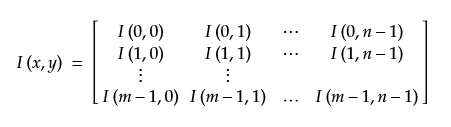
\includegraphics[width=0.8\textwidth]{gambar/image_intensity}
	\caption{Representasi Citra Digital}
	\label{Gambar:imageintensity}
\end{figure}
$m$ x $n$ menyatakan resolusi citra, dan setiap elemen dari matriks menyatakan sebuah piksel (\emph{picture element}). Nilai $I$ pada pasangan koordinat $(x,y)$ disebut intensitas (\emph{intensity}). Dalam operasi pengolahan citra, sebagian besar operasi dilakukan dalam citra \emph{grayscale} \citep{tyagi2018understanding}.

\subsection{Citra \emph{Grayscale}}
Citra \emph{grayscale} adalah citra yang hanya memiliki satu kanal (\emph{channel}) pada setiap pikselnya yang mewakili intensitas. Intensitas piksel berada dalam kisaran [0, 255] yang mana hal ini menunjukkan tingkat terangnya atau tingkat cahaya dari suatu pixel. Warna pada citra \emph{grayscale} merupakan warna abu dengan tingkatan dari hitam hingga sampai putih (tingkat keabuan). Kisaran intensitas piksel bernilai 0 artinya hitam dan 255 adalah putih (untuk \emph{256-graylevel}).
\begin{figure}[H]
	\centering
	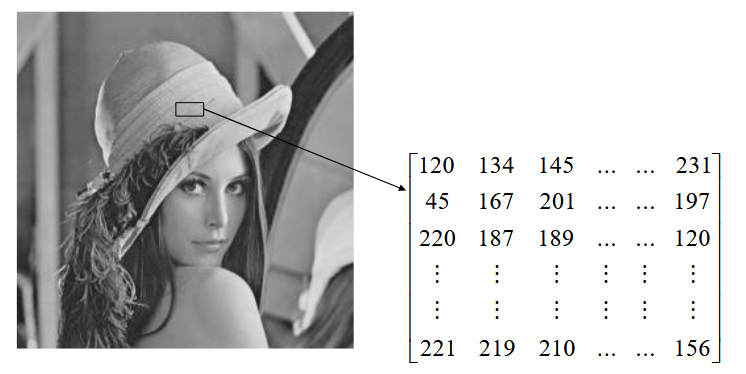
\includegraphics[width=0.5\textwidth]{gambar/grayimage}
	\caption{Contoh citra \emph{grayscale}}
	\label{Gambar:grayimage}
\end{figure}

Setiap piksel dalam citra umumnya dijelaksan oleh kombinasi tiga nilai intensitas R (\emph{red}), G (\emph{green}),dan B (\emph{blue}). Salah satu cara memetakan nilai tersebut ke satu nilai \emph{grayscale} adalah dengan menggunakan metode \emph{luminosity} \citep{kumar2016gray}.
\begin{equation}
	\label{luminosity}
	L(x,y) = 0.21 R (x,y) + 0.72 G (x,y) + 0.07 B (x,y).
\end{equation}
$L(x,y)$ melambangkan nilai intensitas \emph{grayscale} pada pasangan koordinat $(x, y)$. R, G, dan B masing-masing adalah nilai intensites citra \emph{channel} R (\emph{red}), G (\emph{green}),dan B (\emph{blue}) pada pasangan koordinat $(x,y)$

\begin{figure}[H]
	\centering
	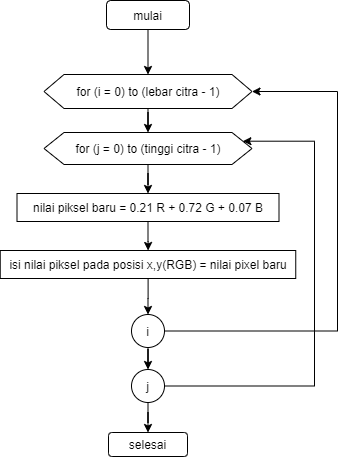
\includegraphics[width=0.45\textwidth]{diagram/grayscale}
	\caption{Proses konversi citra RGB menjadi \emph{grayscale}}
	\label{Gambar:grayscalediagram}
\end{figure}

\subsection{\emph{Gaussian Low Pass Filter} / \emph{Gaussian Filter}}
Peningkatan kualitas citra (\emph{image enhancement}) adalah proses mengedit citra untuk membuatnya 'lebih baik' untuk aplikasi tertentu \citep{tyagi2018understanding}. Hal ini melibatkan proses menghaluskan atau mempertajam konten citra. Salah satu metode dalam proses menghaluskan citra adalah \emph{filtering}, salah satunya adalah dengan menggunakan metode \emph{Gaussian filter}. Proses ini adalah proses memblur citra menggunakan fungsi Gaussian dengan tujuan mengurangi \emph{noise} citra dan mengurangi detail tertentu. Kernel gaussian \emph{Gaussian blur} $G(x,y)$ dideskripsikan sebagai berikut:
\begin{equation}
\label{gaussblur}
G(x,y) = {\frac{1}{2 \pi \sigma^2} e}^{-{\frac{x^2+y^2}{2 \sigma^2}}}
\end{equation}
$\sigma$ dan $e$ menujukkan standar deviasi dan konstanta logaritma natural ($e \approx 2,718281828459$), $x$ dan $y$ adalah posisi koordinat Kernel gaussian.



\section{Gradien citra (\emph{image gradient})}
Tepi (\emph{edge}) dalam ruang lingkup pengolahan citra digital mencirikan batas dari suatu objek dalam citra digital. Deteksi tepi (\emph{edge detection}) merupakan metode identifikasi objek dalam citra berbasis tepi. Salah satu metode deteksi tepi yang umum digunakan adalah metode gradien citra (\emph{image gradient}). Dalam konsep matematis, gradien dikenal sebagai turunan pertama (\emph{first-order derivatives}). Gradien dari citra $I$ dilambangkan dengan notasi $\nabla I$ dan di definisikan sebagai berikut:
\begin{equation}
	\label{gradientimagedefinition}
	{
		\nabla I =
	}
	{
		\begin{bmatrix}
			\nabla I (x,y)_x	\\
			\nabla I (x,y)_y
		\end{bmatrix}
	}
	{
		=
	}
	{
		\begin{bmatrix}
			\frac{\partial I (x,y)}{\partial x}	\\
			\frac{\partial I (x,y)}{\partial y}
		\end{bmatrix}
	}
\end{equation}
di mana $\nabla I (x,y)_x$ dan $\nabla I (x,y)_y$ masing-masing adalah persamaan gradien citra $I$ arah (\emph{direction}) $x$ dan $y$ yang dapat dihitung menggunakan dua persamaan berikut:
\begin{equation}
	\label{gradient_fd1}
	\nabla I (x,y)_x = I(x+1 , y) - I(x,y)
\end{equation}
\begin{equation}
	\label{gradient_fd2}
	\nabla I (x,y)_y = I(x , y + 1) - I(x,y)
\end{equation}
untuk besarnya (\emph{magnitude}) gradien $I$ dapat dihitung menggunakan persamaan berikut:
\begin{equation}
	\label{magnitudegradientfd}
	M(x,y) = ||\nabla I(x,y)|| = \sqrt{ (\nabla I (x,y)_x)^2 + (\nabla I (x,y)_y)^2 }
\end{equation}

Selain menggunakan persamaan (\ref{gradient_fd1}), (\ref{gradient_fd2}), dan (\ref{magnitudegradientfd}), perhitungan gradien citra dapat menggunakan operator gradien yang nantinya akan dikonvolusikan dengan citra. Salah satu operator gradien umum yang sering digunakan adalah operator Sobel/kernel Sobel. Konvolusi dilambangkan dengan $\ast$. Operator Sobel arah $x$ dan $y$, serta besar gradien Sobel masing-masing ditunjukkan oleh persamaan berikut:
\begin{equation}
	\label{sobel_x}
	G_x = 
	\begin{bmatrix}
		-1 & 0 & 1	\\
		-2 & 0 & 2	\\
		-1 & 0 & 1	
	\end{bmatrix}
\end{equation}
\begin{equation}
	\label{sobel_y}
	G_y = 
	\begin{bmatrix}
		1 & 2 & 1	\\
		0 & 0 & 0	\\
		-1 & -2 & -1	
	\end{bmatrix}
\end{equation}
\begin{equation}
	\label{sobel_mag}
	GS = | G_x \ast I(x,y) | + | G_y \ast I(x,y) |
\end{equation}

\begin{figure}[H]
	\centering
	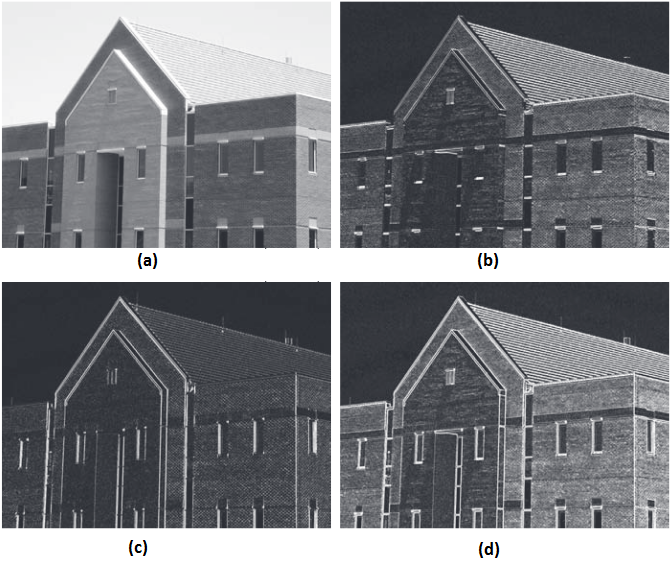
\includegraphics[width=0.8\textwidth]{gambar/sobel}
	\caption{(a) citra \emph{grayscale} ; (b) $|G_x \ast I(x,y)|$, gradien arah $x$ menggunakan kernel Sobel-x ; (c) $|G_y \ast I(x,y)|$, gradien arah $x$ menggunakan kernel Sobel-y ; (d) gradien citra, $| G_x \ast I(x,y) | + | G_y \ast I(x,y) |$ \citep{gonzalez2002digital}}
	\label{Gambar:sobel}
\end{figure}

\section{\emph{Active contour}}
\emph{Active contour} yang juga dikenal dengan sebutan \emph{snakes} adalah kurva yang di definisikan dalam citra (\emph{image}), kurva ini dapat bergerak menuju batas objek atau \emph{feature} dari sebuah citra yang dipengaruhi oleh dua fungsional energi yang disebut energi internal dan energi eksternal.
\begin{figure}[H]
	\centering
	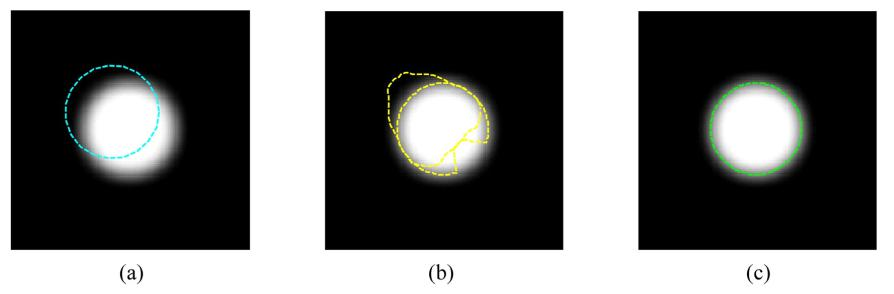
\includegraphics[width=1\textwidth]{gambar/snake1}
	\caption{(a) citra objek lingkaran \& \emph{initial snake}, (b) evolusi kurva \emph{snake},
		(c) bentuk akhir dari \emph{snake} setelah iterasi selesai \citep{acton2007biomedical:19}}
	\label{Gambar:snake1}
\end{figure}

\subsection{Representasi \emph{Snake}}
\emph{Snake} di representasikan sebagai kurva parametrik tertutup $\textbf{v}(s) = (x(s), y(s))$, di mana $s$ adalah panjang kurva dengan rentang tertentu, $x(s)$ dan $y(s)$ masing-masing merupakan elemen dari kurva $\textbf{v}$ pada saat $s$. Sebagai contoh diberikan sebuah kurva sebagai berikut:
\begin{figure}[H]
	\centering
	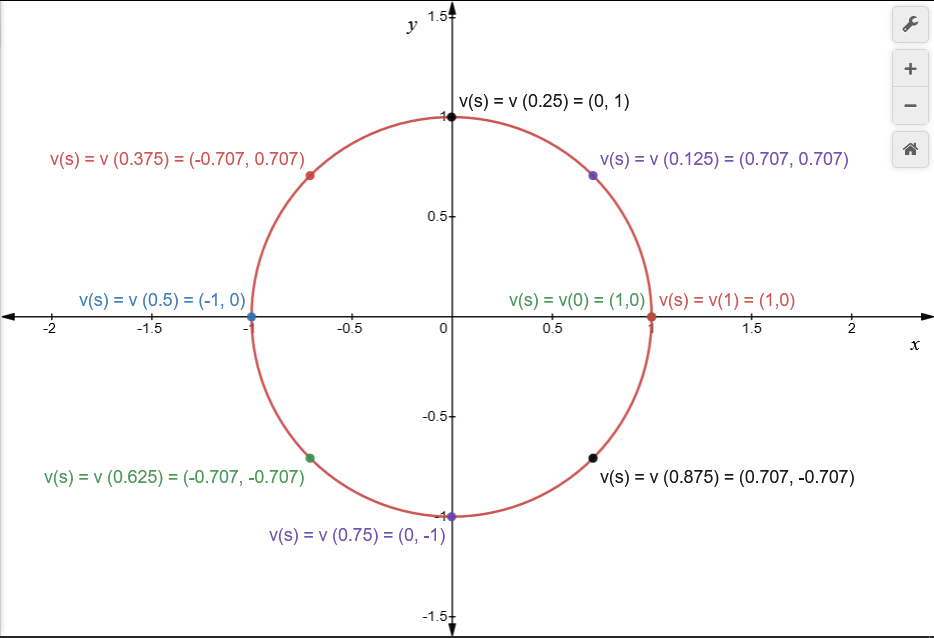
\includegraphics[width=1\textwidth]{gambar/k_lingkaran}
	\caption{Kurva ingkaran}
	\label{Gambar:k_lingkaran}
\end{figure}
Kurva di atas adalah kurva lingkaran $\textbf{v}(s) = [cos (2 \pi s), sin (2 \pi s)]$, $s \in [0, 1]$. Perlu diperhatikan bahwa titik awal $\textbf{v}(0)$ dan titik akhir $\textbf{v}(1)$ di definisikan sebagai titik yang sama.

Algoritma pembuatan lingkaran menggunakan bentuk parametrik (\emph{parametric form}) lingkaran adalah sebagai berikut:
\begin{figure}[H]
	\begin{lstlisting}[language=Python, basicstyle=\tiny]
		repeat until theta >= 360;
		{ 
			x = h + r*cos(theta)
			y = k + r*sin(theta)
			draw a line to x,y
			add step to theta
		}
	\end{lstlisting}
	\caption{\emph{source code} inisialisasi kurva lingkaran}
	\label{Gambar:algo_circle}
\end{figure}
yang dilakukan algoritma di atas adalah menghasilkan koordinat \texttt{x, y} dari sebuah titik pada lingkaran yang diberi sudut (\texttt{theta}). Dimulai dari \texttt{theta = 0} kemudian \emph{looping} sampai \texttt{theta = 360} atau \texttt{theta = $2\pi$}. \texttt{h} dan \texttt{k} adalah koordinat dari titik tengah lingkaran dan \texttt{r} adalah jari-jari lingkaran \citep{john_page}

Fungsional energi \emph{snake} di definisikan sebagai berikut \citep{abdullah2016robust}:
\begin{equation}
	\label{eq_1}
	E_{snake} = \int^1_0 E_{int}(\textbf{v}(s)) ds + \int^1_0 E_{ext}(\textbf{v}(s)) ds.
\end{equation}

\subsection{Energi internal}
Energi internal digunakan untuk mengontrol perubahan bentuk (deformabilitas) dari \emph{snake}, yang ditulis sebagai berikut \citep{abdullah2016robust}:
\begin{equation}
	\label{eq_2}
	E_{int}(\textbf{v}(s)) = \frac{1}{2}  \biggl( \alpha(s)|\textbf{v}_{s}(s)|^2 + \beta(s)|\textbf{v}_{ss}(s)|^2 \biggr)
\end{equation}
$s$ pada $\textbf{v}_{s}$ melambangkan turunan pertama, $ss$ pada $\textbf{v}_{ss}$ melambangkan turunan kedua, dan seterusnya. Fungsi energi internal ini terdiri dari suku pertama yang dikendalikan oleh $\alpha(s)$ dan suku kedua yang dikendalikan oleh $\beta(s)$. Suku pertama mengontrol elastisitas (\emph{elasticity}) dan suku kedua mengontrol kekakuan (\emph{stiffness}) snake. Untuk penyederhanaan, bobot $\alpha(s)$ dan $\beta(s)$ \textbf{diasumsikan seragam}, sehingga $\alpha(s) = \alpha$ dan $\beta(s) = \beta$ hal ini mencegah agar deformabilitas snake tidak membentuk sudut \citep{ivins1995everything}. Tidak ada aturan dalam menentukan $\alpha$ dan $\beta$, tetapi yang perlu diperhatikan adalah semakin kecil nilai $\alpha$ mengakibatkan jarak tiap titik pada kurva semakin tidak teratur dan sebaliknya semakin besar nilai $\alpha$ mengakibatkan jarak tiap titik pada kurva semakin teratur. Untuk parameter $\beta$, semakin kecil nilainya akan menyebabkan bentuk kurva menjadi semakin tidak \emph{smooth} atau dapat membentuk sudut dan sebaliknya semakin besar nilai $\beta$ menyebabkan kurva semakin \emph{smooth} \citep{ickhsan2020implementasi}.

\subsection{Energi eksternal}
Energi internal berasal dari kurva \emph{snake}, sedangkan energi eksternal berasal dari luar yakni dari citra itu sendiri.

Jika diberikan citra tingkat abu-abu (\emph{gray-level image}) $I (x, y)$, maka fungsi energi eksternal yang sesuai meliputi \citep{xu1998snakes:22}:
\begin{equation}
	\label{eext1}
	E^{(1)}_{ext}(x,y) = -|\nabla I(x,y)|^2
\end{equation}
\begin{equation}
	\label{eext2}
	E^{(2)}_{ext}(x,y) =  -|\nabla \left[ G_{\sigma} (x,y) * I(x,y) \right]|^2
\end{equation}
Jika citra tersebut adalah citra biner (\emph{black-white}), energi eksternal yang sesuai di antaranya adalah sebagai berikut:
\begin{equation}
	\label{eext3}
	E^{(3)}_{ext}(x,y) = I(x,y)
\end{equation}
\begin{equation}
	\label{eext4}
	E^{(4)}_{ext}(x,y) = G_{\sigma} (x,y) * I(x,y)
\end{equation}
di mana $G_{\sigma}(x,y)$ adalah fungsi \emph{Gaussian} dengan standar deviasi $\sigma$, $\nabla$ adalah operator gradien. $\ast$ mewakili konvolusi $G_{\sigma}(x,y) \ast I(x,y)$, di mana $I(x,y)$ adalah fungsi intensitas citra. $\nabla$ adalah operator gradien, kita dapat menggunakan operator Sobel pada persamaan (\ref{sobel_x}) dan (\ref{sobel_y}) untuk menjalankan fungsi energi eksternal ini.

Substitusi Energi internal (\ref{eq_2}) dan Energi Eksternal (\ref{eext1}) - (\ref{eext4}) ke fungsional energi \emph{snake} (\ref{eq_1}), menghasilkan persamaan energi \emph{snake} menjadi:
\begin{multline}
\label{eq_4}
E_{snake} = \int^{1}_{0} \Biggl( \frac{1}{2} \biggl(\alpha(s)|\textbf{v}_{s}(s)|^2 + \beta(s)|\textbf{v}_{ss}(s)|^2\biggr) + E^{(i)}_{ext}(x,y) \Biggr) ds.
\end{multline}
dengan $i = 1,2,3,4$.




\section{\emph{Active contour evolution}}
Kurva \emph{snake} akan bergerak menuju batas dari \emph{feature} dari sebuah citra, proses ini disebut \emph{active contour evolution}. Perhitungan evolusi \emph{snake} yang meminimalkan persamaan energi (\ref{eq_4}) ketika $\alpha(s) = \alpha$ dan $\beta(s) = \beta$, harus memenuhi persamaan Euler berikut \citep{xu1998snakes:22}:
\begin{equation}
	\label{snake_euler}
	\alpha\textbf{v}_{ss}(s) - \beta\textbf{v}_{ssss}(s) + \nabla E^{(i)}_{ext}  = 0
\end{equation}
Untuk menemukan solusi persamaan (\ref{snake_euler}), kurva snake $\textbf{v}$ dibuat dinamis terhadap waktu $t$. Turunan parsial $\textbf{v}$ terhadap $t$ ditetapkan sama dengan ruas kiri persamaan (\ref{snake_euler}) sebagai berikut \citep{xu1998snakes:22}:
\begin{equation}
	\label{snake_euler_t}
	\textbf{v}_{t}(s,t) = \alpha\textbf{v}_{ss}(s,t) - \beta\textbf{v}_{ssss}(s,t) + \nabla E^{(i)}_{ext}  = 0
\end{equation}
atau dapat ditulis sebagai berikut \citep{ivins1995everything}:
\begin{equation}
	\label{snake_euler_t_partial}
	\frac{\partial\textbf{v}}{\partial t} = \alpha \frac{\partial^2 \textbf{v}}{\partial s^2} - \beta \frac{\partial^4 \textbf{v}}{\partial s^4} + \frac{\partial E^{(i)}_{ext} }{ \partial \textbf{v}} = 0
\end{equation}
$\textbf{v}$ pada persmaan (\ref{snake_euler_t_partial}) dapat dipisahkan menjadi komponen/elemen $x$ dan $y$, katakanlah $u_{j}$ adalah komponen/elemen \emph{snake} $\textbf{v}$ di mana $j = 0,1,.., N-1$ sebagai aproksimasi diskrit untuk $x(s)$ dan $y(s)$, dan $t$ melambangkan iterasi, maka persamaan (\ref{snake_euler_t_partial}) menjadi:
\begin{equation}
	\label{snake_euler_t_partial_u}
	\frac{\partial u^{t}_{j} }{\partial t} = \alpha \frac{\partial^2 u^{t}_{j}}{\partial s^2} - \beta \frac{\partial^4 u^{t}_{j}}{\partial s^4} + \frac{\partial E^{(i)}_{ext} }{ \partial u^{t}_{j}} = 0
\end{equation}
Turunan pada persamaan (\ref{snake_euler_t_partial_u}) dapat diaproksimasikan menggunakan \emph{finite differences} yang ditunjukan pada gambar berikut:
\begin{figure}[H]
	\centering
	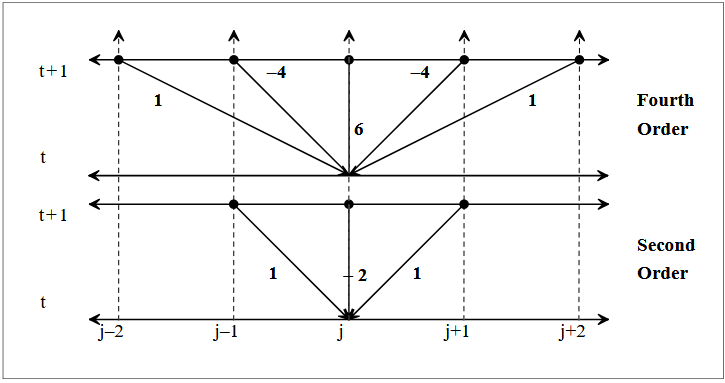
\includegraphics[width=1\textwidth]{gambar/finite_d}
	\caption{Aproksimasi turunan dengan \emph{finite differences} \citep{ivins1995everything}}
	\label{Gambar:finite_d}
\end{figure}
Turunan $\frac{\partial u^{t}_{j} }{\partial t}$ diaproksimasikan menjadi $\dfrac{ u^{t+1}_j - u^{t}_j }{\delta t}$ \citep{ivins1995everything}. Turunan orde kedua, yaitu $\frac{\partial^2 u^{t}_{j}}{\partial s^2}$ diaproksimasikan menjadi $\frac{( u^{t+1}_{j+1} + u^{t+1}_{j-1} - 2u^{t+1}_{j} )}{\delta s^2}$, sedangkan turunan orde keempat, yaitu $\frac{\partial^4 u^{t}_{j}}{\partial s^4}$ diaproksimasikan menjadi $\frac{( u^{t+1}_{j+2} - 4u^{t+1}_{j+1} + 6u^{t+1}_{j} - 4u^{t+1}_{j-1} + u^{t+1}_{j-2})}{\delta s^4}$.
Turunan dalam persamaan (\ref{snake_euler_t_partial_u}) yang diaproksimasi menggunakan \emph{finite differences} seperti yang ditunjukkan pada Gambar (\ref{Gambar:finite_d}) adalah sebagai berikut:

\begin{multline}
	\label{aprox_finite}
	\dfrac{ u^{t+1}_j - u^{t}_j }{\delta t} = \frac{\alpha}{\delta s^2}( u^{t+1}_{j+1} + u^{t+1}_{j-1} - 2u^{t+1}_{j} ) \\
	- \frac{\beta}{\delta s^4}( u^{t+1}_{j+2} - 4u^{t+1}_{j+1} + 6u^{t+1}_{j} - 4u^{t+1}_{j-1} + u^{t+1}_{j-2}) + \frac{\partial E^{(i)}_{ext} }{ \partial u^{t}_{j}}
\end{multline}

\begin{comment}
\begin{multline}
	\label{aprox_finite1}
	u^{t+1}_j - u^{t}_j = \frac{\alpha \delta t}{\delta s^2} u^{t+1}_{j+1} + \frac{\alpha \delta t}{\delta s^2} u^{t+1}_{j-1} - \frac{\alpha \delta t}{\delta s^2} 2u^{t+1}_{j} \\
	- \frac{\beta \delta t}{\delta s^4} u^{t+1}_{j+2} + \frac{\beta \delta t}{\delta s^4} 4u^{t+1}_{j+1} - \frac{\beta \delta t}{\delta s^4} 6u^{t+1}_{j} + \frac{\beta \delta t}{\delta s^4} 4u^{t+1}_{j-1} - \frac{\beta \delta t}{\delta s^4} u^{t+1}_{j-2} - \frac{\partial E^{(i)}_{ext} \delta t}{ \partial u^{t}_{j}}
\end{multline}

\begin{multline}
	\label{aprox_finite2}
	u^{t+1}_j - u^{t}_j = \frac{\alpha \delta t}{\delta s^2} u^{t+1}_{j+1} + \frac{\alpha \delta t}{\delta s^2} u^{t+1}_{j-1} - \frac{\alpha \delta t}{\delta s^2} 2u^{t+1}_{j} \\
	- \frac{\beta \delta t}{\delta s^4} u^{t+1}_{j+2} + \frac{\beta \delta t}{\delta s^4} 4u^{t+1}_{j+1} - \frac{\beta \delta t}{\delta s^4} 6u^{t+1}_{j} + \frac{\beta \delta t}{\delta s^4} 4u^{t+1}_{j-1} - \frac{\beta \delta t}{\delta s^4} u^{t+1}_{j-2} - \frac{\partial E^{(i)}_{ext} \delta t}{ \partial u^{t}_{j}}
\end{multline}
\end{comment}


di mana $t$ dan $t+1$ mewakili parameter waktu yang berurutan dengan langkah waktu (\emph{time step}) $\delta t$. $\delta s$ mewakili ukuran langkah (\emph{step size}). Mememindahkan $\delta t$ ke ruas kanan persamaan membuat persamaan (\ref{aprox_finite}) menjadi:
\begin{multline}
	\label{aprox_finite_LHS}
	b u^{t+1}_{j+2} - (a+4b) u^{t+1}_{j+1} + (1+2a+6b) u^{t+1}_{j} - (a+4b) u^{t+1}_{j-1} + b u^{t+1}_{j-2} \\
	= u^{t}_{j} + \delta t \frac{\partial E^{(i)}_{ext} }{ \partial u^{t}_{j}}
\end{multline}
di mana $a \equiv \alpha \frac{\delta t}{\delta s^2} $ dan $b \equiv \beta \frac{\delta t}{\delta s^4} $.
Persamaan (\ref{aprox_finite_LHS}) dapat juga ditulis sebagai berikut:
\begin{equation}
	\label{aprox_finite_rhs}
	p u^{t+1}_{j+2} + q u^{t+1}_{j+1} + r u^{t+1}_{j} + q u^{t+1}_{j-1} + p u^{t+1}_{j-2} \\
	= \tilde{u}^{t+1}_{j}
\end{equation}
di mana $p \equiv b$, $q \equiv -a-4b$, dan $r \equiv 1+2a+6b$, sedangkan $\tilde{u}^{t+1}_{j} = u^{t}_{j} + \delta t \frac{\partial E^{(i)}_{ext} }{ \partial u^{t}_{j}}$. Persamaan (\ref{aprox_finite_rhs}) ini dapat ditulis dalam bentuk matriks untuk koordinat $x$ dan $y$ dari setiap elemen kurva \emph{snake} $\textbf{v}$.



\begin{equation}
	\label{matriks_implicit}
	{
		\begin{bmatrix}
			r 	& q			& p 	 & 		  & 	   & p 		& q \\
			q 	& r     	& q 	 & 	p	  & 	   &  		& p \\
			p 	& q     	& r 	 & 	q	  & p	   &  		&  	\\
			& \ddots 	& \ddots & \ddots & \ddots & \ddots &  	\\
			&  			& p 	 & 	q	  & r	   & q 		& p \\
			p 	&  			& 	 	 & 	p	  & q	   & r 		& q \\
			q 	& p 		&  		 & 		  & p	   & q 		& r
		\end{bmatrix}
	}
	{
		\begin{bmatrix}
			u^{t+1}_{0} 	\\
			u^{t+1}_{1} 	\\
			u^{t+1}_{2} 	\\
			\vdots 			\\
			u^{t+1}_{N-3}\\
			u^{t+1}_{N-2}\\
			u^{t+1}_{N-1}
		\end{bmatrix}
	}
	{
		=
	}
	{
		\begin{bmatrix}
			\tilde{u}^{t+1}_{0} 	\\
			\tilde{u}^{t+1}_{1} 	\\
			\tilde{u}^{t+1}_{2} 	\\
			\vdots 					\\
			\tilde{u}^{t+1}_{N-3}	\\
			\tilde{u}^{t+1}_{N-2}	\\
			\tilde{u}^{t+1}_{N-1}
		\end{bmatrix}
	}
\end{equation}
di mana

\begin{equation}
	\label{matriks_m}
	{
		\textbf{M} =
	}
	{
		\begin{bmatrix}
			r 	& q			& p 	 & 		  & 	   & p 		& q \\
			q 	& r     	& q 	 & 	p	  & 	   &  		& p \\
			p 	& q     	& r 	 & 	q	  & p	   &  		&  	\\
			& \ddots 	& \ddots & \ddots & \ddots & \ddots &  	\\
			&  			& p 	 & 	q	  & r	   & q 		& p \\
			p 	&  			& 	 	 & 	p	  & q	   & r 		& q \\
			q 	& p 		&  		 & 		  & p	   & q 		& r
		\end{bmatrix}
	}
\end{equation}

\begin{equation}
	\label{matriks_ut1}
	{
		\textbf{u}^{t+1}_{j} =
	}
	{
		\begin{bmatrix}
			u^{t+1}_{0} 	\\
			u^{t+1}_{1} 	\\
			u^{t+1}_{2} 	\\
			\vdots 			\\
			u^{t+1}_{N-3}\\
			u^{t+1}_{N-2}\\
			u^{t+1}_{N-1}
		\end{bmatrix}
	}
\end{equation}

\begin{equation}
	\label{matriks_ut2}
	{
		\tilde{\textbf{u}}_{j}^{t+1} =
	}
	{
		\begin{bmatrix}
			\tilde{u}^{t+1}_{0} 	\\
			\tilde{u}^{t+1}_{1} 	\\
			\tilde{u}^{t+1}_{2} 	\\
			\vdots 					\\
			\tilde{u}^{t+1}_{N-3}	\\
			\tilde{u}^{t+1}_{N-2}	\\
			\tilde{u}^{t+1}_{N-1}
		\end{bmatrix}
	}
	{
		=
	}
	{
		\begin{bmatrix}
			u^{t}_{0} + \delta t \frac{\partial E^{(i)}_{ext} }{ \partial u^{t}_{0}} 	\\
			u^{t}_{1} + \delta t \frac{\partial E^{(i)}_{ext} }{ \partial u^{t}_{1}} 	\\
			u^{t}_{2} + \delta t \frac{\partial E^{(i)}_{ext} }{ \partial u^{t}_{2}} 	\\
			\vdots 					\\
			u^{t}_{N-3} + \delta t \frac{\partial E^{(i)}_{ext} }{ \partial u^{t}_{N-3}}	\\
			u^{t}_{N-2} + \delta t \frac{\partial E^{(i)}_{ext} }{ \partial u^{t}_{N-2}}	\\
			u^{t}_{N-1} + \delta t \frac{\partial E^{(i)}_{ext} }{ \partial u^{t}_{N-1}}
		\end{bmatrix}
	}
	%{
	%	=
	%}
	%{
	%	u^{t}_{j} - \delta t \frac{\partial E^{(i)}_{ext} }{ \partial u^{t}_{j}}
	%}
\end{equation}

\begin{equation}
	\label{consteq}
	p \equiv \beta \frac{\delta t}{\delta s^4}, q \equiv - \alpha \frac{\delta t}{\delta s^2} - 4 \beta \frac{\delta t}{\delta s^4}, r \equiv  1 + 2 \alpha \frac{\delta t}{\delta s^2} + 6 \beta \frac{\delta t}{\delta s^4}
\end{equation}
Mengalikan kedua sisi dari persamaan (\ref{matriks_implicit}) dengan inverse dari matriks $\textbf{M}$ memberikan solusi akhir persamaan \emph{snake} menjadi:
\begin{equation}
	\label{implicit}
	\textbf{u}^{t+1}_{j} = \textbf{M}^{-1} \biggl( \textbf{u}^t_{j} + \delta t  \frac{\partial E^{(i)}_{ext} }{ \partial \textbf{u}^{t}_{j}} \biggr)
\end{equation}

Perlu diingat $\textbf{u}$ adalah komponen/elemen $x$ dan $y$ pada kurva \emph{snake}, komponen/elemen ini dapat dinyatakan dengan vektor $\textbf{x}$ dan $\textbf{y}$. Jika $E^{(i)}_{ext}$ dinotasikan menjadi fungsi $\textbf{f}$ maka :
\begin{equation}
	\label{ext_f}
	\frac{\partial E^{(i)}_{ext} }{ \partial \textbf{u}^{t}_{j}} = \frac{\partial \textbf{f} }{ \partial \textbf{u}^{t}_{j}}
\end{equation}

Hal ini membuat persamaan (\ref{implicit}) dapat ditulis sebagai berikut:
\begin{equation}
	\label{implicit_x}
	\textbf{x}^{t+1}_{j} = \textbf{M}^{-1} \biggl( \textbf{x}^t_{j} + \delta t \; \textbf{f}_{x} \biggr)
\end{equation}
dan
\begin{equation}
	\label{implicit_y}
	\textbf{y}^{t+1}_{j} = \textbf{M}^{-1} \biggl( \textbf{y}^t_{j} + \delta t \; \textbf{f}_{y} \biggr)
\end{equation}

$\textbf{f}_x$ dan $\textbf{f}_y$ adalah vektor-vektor yang bersesuaian dengan bentuk turunan pertama $\frac{\partial \textbf{f} }{ \partial \textbf{u}^{t}_{j}}$ sebagai berikut:
\begin{equation}
	\label{fx_eq}
	% \textbf{f}_x = f_x(x^t_{j}, y^t_{j}) = f(x^t_{j}+1) , y^t_{j}) - f(x^t_{j},y^t_{j})
	\textbf{f}_x = f_x(x^t_{j}, y^t_{j})
\end{equation}

\begin{equation}
	\label{fy_eq}
	% \textbf{f}_y = f_y(x^t_{j}, y^t_{j}) = f(x^t_{j}, y^t_{j}+1) - f(x^t_{j},y^t_{j})
	\textbf{f}_y = f_y(x^t_{j}, y^t_{j})
\end{equation}
di mana $x^t_{j}$ dan $y^t_{j}$ adalah pasangan koordinat dari kurva \emph{snake}. $\textbf{f}_x$ dan $\textbf{f}_y$ dapat dicari menggunakan teori gradien citra.
%--algoritma ,equilibrium--

\section{Interpolasi Bilinear}
Interpolasi Bilinear adalah metode interpolasi fungsi dari dua variabel (misal $x$ dan $y$). Metode ini biasanya digunakan untuk mengaproksimasi nilai data di antara beberapa titik dalam \emph{2D rectangular grid}, misalnya di dalam matriks \citep{william1997numerical}.

Misal kita ingin mencari nilai fungsi $f$ yang tidak diketahui di titik $(x,y)$ dan diasumsikan kita mengetahui nilai $f$ pada beberapa empat titik $Q_11 = (x_1, y_1), Q_12 = (x_1, y_2), Q_21 = (x_2, y_1), dan Q_22 = (x_2, y_2)$ maka langkah yang harus dilakukan sebagai berikut:
\begin{equation}
	\label{bilin_x1}
	f(x,y_1) = \frac{x_2 - x}{x_2 - x1} f(Q_11) + \frac{x - x_1}{x_2 - x_1} f(Q_21) = R1
\end{equation}

\begin{equation}
	\label{bilin_x2}
	f(x,y_2) = \frac{x_2 - x}{x_2 - x1} f(Q_12) + \frac{x - x_1}{x_2 - x_1} f(Q_22) = R2
\end{equation}

\begin{equation}
	\label{bilin_y}
	f(x,y) = \frac{y_2 - y}{y_2 - y_1} f(x, y_1) + \frac{y - y_1}{y_2 - y_1} f(x, y_2) = P
\end{equation}

\begin{figure}[H]
	\centering
	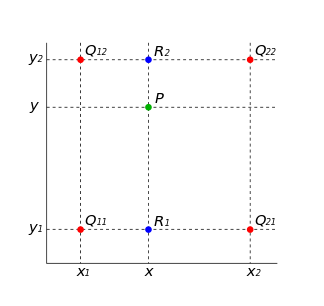
\includegraphics[width=.7\textwidth]{gambar/bilinear_interpolation}
	\caption{interpolasi bilinear}
	\label{Gambar:bilin_ilust}
\end{figure}


\begin{comment}

\section{\emph{Gradient Vector Flow (GVF) snake}}
Model \emph{snake} tradisional memiliki kekurangan seperti yang dibahas sebelumnya. Sebagian besar alasan kinerja yang buruk dikaitkan dengan energi eksternal. Untuk memperbaiki masalah ini, \citep{xu1998snakes:22} mengusulkan energi eksternal baru yang dikenal sebagai GVF \emph{snake} . 

Model dasar GVF sama dengan persamaan \emph{snake} (\ref{snake_euler_t}), tetapi yang membedakan adalah energi eksternal $- \nabla E^{(i)}_{ext}$ yang di definisikan menjadi $\textbf{g}$ sebagai berikut:
\begin{equation}
	\label{gvf_euler_t}
	\textbf{v}_{t}(s,t) = \alpha\textbf{v}_{ss}(s,t) - \beta\textbf{v}_{ssss}(s,t) + \textbf{g}  = 0
\end{equation}
di mana $\textbf{g}(x, y) = [ u (x, y), v (x, y) ]$ adalah bidang vektor(\emph{vector field}), \emph{field} ini dapat dianggap sebagai \textbf{vektor gradien} dari citra (\emph{gray-level} atau \emph{binary edge-map}) \citep{xu1998snakes:22}.

\subsection{Peta Tepi (\emph{Edge Map})}
Langkah pertama untuk mendapatkan GVF adalah mendefinisikan fungsi \emph{edge map} $f(x,y)$ yang berasal dari citra $I(x,y)$. Kita dapat menggunakan peta tepi \emph{gray-level} atau \emph{binary} sesuai yang kita tentukan berdasarkan energi eksternal \emph{snake} dasar pada persamaan (\ref{eext1}) - (\ref{eext4}) sebagai berikut:
\begin{equation}
	\label{gvf_edge_map}
	f(x,y) = - E^{(i)}_{ext}(x,y)
\end{equation}
dengan $i = 1,2,3,4$.


%================|||||=====================



\subsection{\emph{Gradient Vector Flow}}
\emph{GVF} di definisikan sebagai vektor gradien $\textbf{g}(x,y) = [u(x,y), v(x,y)]$ yang meminimalkan fungsional energi sebagai berikut
\begin{equation}
	\label{equ_gvf}
	\varepsilon = \int \int \mu (u_x^2 + u_y^2 + v_x^2 + v_y^2) + |\nabla f|^2 |\textbf{g} - \nabla f|^2 \,\, dx dx
\end{equation}
di mana $\nabla f$ adalah gradien dari \emph{edge map}. $\mu$ adalah parameter regularisasi (\emph{regularization parameter}) yang menyesuaikan antara suku pertama dan suku kedua. Parameter $\mu$ dikenal sebagai pemulusan (\emph{smoothing term}) dan data(\emph{data term}). Nilai $\mu$ bergantung pada tingkat kebisingan(\emph{noise}) yang ada pada citra $I$, yaitu semakin tinggi \emph{noise}, nilai $\mu$ sebaiknya ditingkatkan\citep{xu1998snakes:22}.

Persamaan (\ref{equ_gvf}) bukan merupakan bentuk akhir karena masih dalam bentuk integran. Untuk mencari nilai $\textbf{g}$, dua persamaan Euler dibawah ini harus diselesaikan:
\begin{equation}
	\label{equ_gvf_a1}
	\mu {\nabla}^2 u - (u - f_x) (f_x^2 + f_y^2) = 0
\end{equation}
dan
\begin{equation}
	\label{equ_gvf_a2}
	\mu {\nabla}^2 v - (v - f_y) (f_x^2 + f_y^2) = 0
\end{equation}
dengan ${\nabla}^2$ adalah operator Laplacian. Untuk menghitung $f_x$ dan $f_y$ dapat menggunakan operator gradien umum seperti operator Sobel pada persamaan (\ref{sobel_x}) dan (\ref{sobel_y}). Kedua persamaan di atas dapat diselesaikan dengan menjadikan $u$ dan $v$ sebagai fungsi waktu $t$ sebagai berikut:
\begin{equation}
	\label{equ_gvf_b1}
	u_t(x,y,t) = \mu {\nabla}^2 u(x,y,t) - [ u(x,y,t) - f_x(x,y) ] [ f^2_x (x,y) + f_y^2(x,y) ]
\end{equation}
dan
\begin{equation}
	\label{equ_gvf_b2}
	v_t(x,y,t) = \mu {\nabla}^2 v(x,y,t) - [ v(x,y,t) - f_y(x,y) ] [ f^2_x (x,y) + f_y^2(x,y) ]
\end{equation}
Persamaan (\ref{equ_gvf_b1}) dan (\ref{equ_gvf_b2}) dapat ditulis ulang sebagai berikut :
\begin{equation}
	\label{gvf_t1}
	u_t(x,y,t) = \mu {\nabla}^2 u(x,y,t) - b(x,y) u(x,y,t) + c^1(x,y)
\end{equation}
dan
\begin{equation}
	\label{gvf_t2}
	v_t(x,y,t) = \mu {\nabla}^2 v(x,y,t) - b(x,y) u(x,y,t) + c^2(x,y)
\end{equation}
di mana
\begin{equation}
	\label{gvf_b}
	b (x,y) = f_x(x,y)^2 + f_y(x,y)^2
\end{equation}
\begin{equation}
	\label{gvf_c1}
	c^1 (x,y) = b(x,y) f_x(x,y)
\end{equation}
\begin{equation}
	\label{gvf_c2}
	c^2 (x,y) = b(x,y)f_y(x,y)
\end{equation}
Untuk solusi iteratif, atur jarak antar piksel menjadi $\Delta x$ dan $\Delta y$, dan langkah waktu(\emph{time step}) untuk setiap iterasi adalah $\Delta t$. Maka selanjutnya dapat diaproksimasikan sebagai berikut\citep{xu1998snakes:22}:
\begin{equation}
	\label{gvf_ut}
	u_t = \frac{1}{\Delta t} ( u^{t+1}_{x,y} - u^t_{x,y} )
\end{equation}
\begin{equation}
	\label{gvf_vt}
	v_t = \frac{1}{\Delta t} ( v^{t+1}_{x,y} - v^n_{x,y} )
\end{equation}
\begin{equation}
	\label{gvf_laplace_u}
	\nabla^2 u = \frac{1}{\Delta x \Delta y} ( u_{x+1,y} + u_{x,y+1} + u_{x-1,y} + u_{x,y-1} - 4u_{x,y} )
\end{equation}
\begin{equation}
	\label{gvf_laplace_v}
	\nabla^2 v = \frac{1}{\Delta x \Delta y} ( v_{x+1,y} + v_{x,y+1} + v_{x-1,y} + v_{x,y-1} - 4v_{x,y} )
\end{equation}
substitusi notasi di atas ke persamaan (\ref{gvf_t1}) dan (\ref{gvf_t2}) memberikan solusi iteratif sebagai berikut
\begin{equation}
	\label{gvfc1}
	u^{t+1}_{x,y} = (1 - b_{i,j} \Delta t) u^{t}_{x,y} + r ( u^{t}_{x+1 , y} + u^t_{x,y+1} + u^t_{x-1 , y} + u^t_{x, y-1} - 4u^t_{x, y}) + c^1_{x,y} \Delta t
\end{equation}
dan
\begin{equation}
	\label{gvfc2}
	v^{t+1}_{x,y} = (1 - b_{x,y} \Delta t) v^{t}_{x,y} + r ( v^{t}_{x+1 , y} + v^n_{x,y+1} + v^t_{x-1 , y} + v^t_{x, y-1} - 4v^t_{x, y}) + c^2_{x,y} \Delta t
\end{equation}
di mana
\begin{equation}
	\label{gvf_r}
	r = \frac{ \mu \Delta t}{\Delta x \Delta y}
\end{equation}
% Selanjutnya jika $\Delta x$, $\Delta y$ dan $\mu$ konstan, maka nilai $\Delta t$ harus memenuhi \citep{CartasAyala2011GradientVF}:
Selanjutnya jika $\Delta x$, $\Delta y$ dan $\mu$ konstan, maka nilai $\Delta t$ harus memenuhi:
\begin{equation}
	\label{gvfnot5}
	\Delta t \leq \frac{\Delta x \Delta y}{4 \mu}
\end{equation}

Selanjutnya dengan mengganti bentuk energi eksternal \emph{snake} dasar masing-masing dengan $u$ dan $v$, persamaan evolusi \emph{snake} (\ref{implicit_x}) dan (\ref{implicit_y})menjadi:
\begin{equation}
	\label{implicit_gvf_u}
	\textbf{x}^{t+1} = \textbf{M}^{-1} \biggl( \textbf{x}^t + \delta t \; u^{t+1}_{x,y} \biggr)
\end{equation}
dan
\begin{equation}
	\label{implicit_gvf_y}
	\textbf{y}^{t+1} = \textbf{M}^{-1} \biggl( \textbf{y}^t + \delta t \; v^{t+1}_{x,y} \biggr)
\end{equation}


berikut adalah ilustrasi dari GVF \emph{snake}:
\begin{figure}[H]
	\centering
	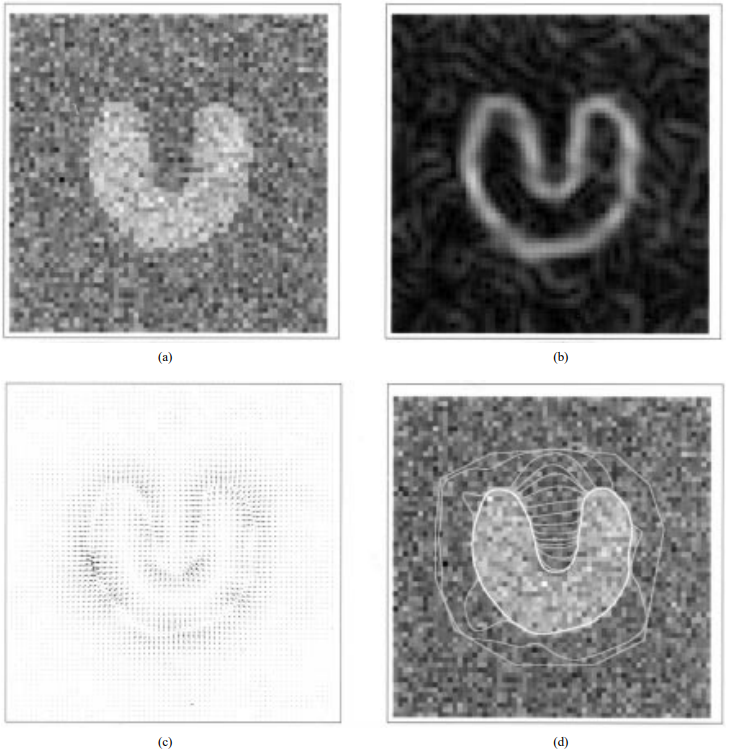
\includegraphics[width=.7\textwidth]{gambar/gvfilu}
	\caption{(a) citra objek U yang memiliki \emph{noise}; (b) \emph{edge map}; (c) medan gaya eksternal GVF; dan (d) konvergensi GVF \emph{snake} \citep{xu1998snakes:22}.}
	\label{Gambar:gvfilu}
\end{figure}

\end{comment}

% Baris ini digunakan untuk membantu dalam melakukan sitasi
% Karena diapit dengan comment, maka baris ini akan diabaikan
% oleh compiler LaTeX.
\begin{comment}
bibliography{daftar-pustaka}
\end{comment}

%!TEX root = ./template-skripsi.tex
%-------------------------------------------------------------------------------
%                            BAB III
%               			PEMBAHASAN
%-------------------------------------------------------------------------------

\chapter{METODOLOGI PENELITIAN}
Berikut ini diagram alir penelitian yang akan dilakukan:
%Selanjutnya kontur akhir akan di bandingkan dengan \emph{ground truth} menggunakan perhitungan \emph{matching similarity} antara 2 citra.
\begin{figure}[H]
	\centering
	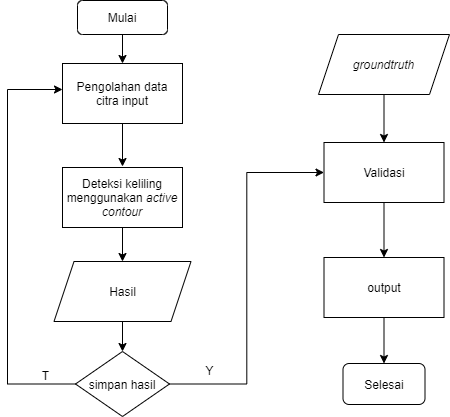
\includegraphics[width=0.6\textwidth]{diagram/metodepenelitian_alur}
	\caption{Diagram alir penelitian}
	\label{Gambar:metodepenelitian_alur}
\end{figure}

\section{Pengolahan data citra input}
Sampel yang baik adalah sampel yang mencerminkan populasinya \citep{amirullah2015metode}. Permata menggunakan data sebanyak 20 citra preparat darah pada penelitiannya tentang segmentasi parasit malaria menggunakan \emph{snake}\citep{permata2015penggunaan}, lalu pada penelitian lain Fadillah menggunakan data sebanyak 15 citra CT-Scan paru-paru pada penelitiannya tentang segmentasi citra paru-paru menggunakan \emph{snake}, dan Constantia menggunakan 21 data citra sapi dalam penelitiannya tentang estimasi bobot sapi menggunakan \emph{snake}\citep{constantia2019estimasi}. 
\begin{comment}
	Tujuan dari sebuah riset adalah untuk memperoleh informasi dari populasi. Populasi merupakan seluruh kumpulan elemen yang dapat digunakan untuk membuat kesimpulan tertentu sedangkan sampel merupakan kelompok yang dipilih dari populasi untuk digunakan dalam riset. Sampai saat ini belum ada kesepakatan atau ketentuan secara ideal dalam menentukan berapa banyak sampel dalam penelitian. 
\end{comment}

% sekaligus sebagai sampel (sampel = populasi), diujikan > tersedia
% mengurangi similarity (luka hitam 1.jpg)
% 28 -> 27 citra, 78 -> 77 citra
\emph{Dataset} luka yang penulis dapat berjumlah 108, sebanyak 37 data tidak dapat dipakai karena data tersebut memiliki duplikasi dengan data lain sehingga data yang tersedia berjumlah 71 buah citra luka yang penulis jadikan sebagai populasi sekaligus sebagai sampel penelitian (sampel = populasi) dengan kategori luka hitam sebanyak 24 citra, luka kuning sebanyak 15 citra, dan luka merah sebanyak 32 citra. \emph{Dataset} ini didapat dari penelitian luka \mbox{Ns. Ratna Aryani, M.Kep}, tahun 2018 \mbox{\citep{ratna2018rancang}} yang tersedia di \emph{repository} \url{https://github.com/mekas/InjuryDetection}. Data yang penulis gunakan adalah data-data yang berekstensi .xcf yang dapat dibuka dengan \emph{software} GIMP, pemrosesan data sebelum deteksi menggunakan \emph{snake} dan GVF dilakukan menggunakan \emph{software} GIMP. \emph{Dataset} ini masing-masing di dalamnya terdapat \emph{layer} citra (luka), \emph{layer} region (luka), dan \emph{path} sebagai berikut :
\begin{figure}[H]
	\centering
	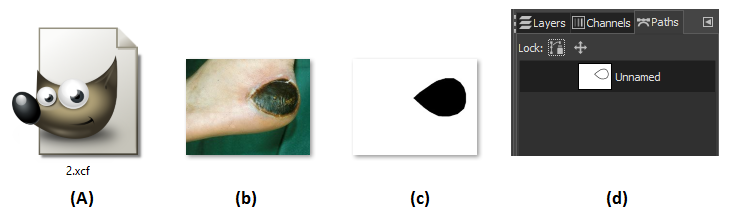
\includegraphics[width=1\textwidth]{gambar/isi_file_xcf}
	\caption{(a) Data citra format .xcf, (b) \emph{layer} citra (luka), (c) \emph{layer} region, (d) \emph{path} }
	\label{Gambar:isi_file_xcf}
\end{figure}

langkah selanjutnya adalah mengubah ukuran (\emph{resize}) citra \emph{size} yang besar ke ukuran yang lebih kecil agar proses deteksi menjadi lebih cepat. Penulis mengubah ukuran citra menggunakan fitur \emph{rescale image} sehingga ukuran citra tidak lebih dari 2 \emph{megabyte}. Kemudian penulis mengecek masing-masing citra dengan fitur \emph{eclipse select} untuk mengetahui apakah objek luka pada data citra pas berada di dalam lingkaran yang akan dijadikan sebagai inisialisasi awal. Ukuran lingkaran tidak boleh lebih besar dari ukuran citra. Jika ukuran lingkaran lebih besar daripada ukuran citra, maka perlu ditambahkan \emph{border} yang dibuat menggunakan fitur \emph{add border} sebagai berikut :
\begin{figure}[H]
	\centering
	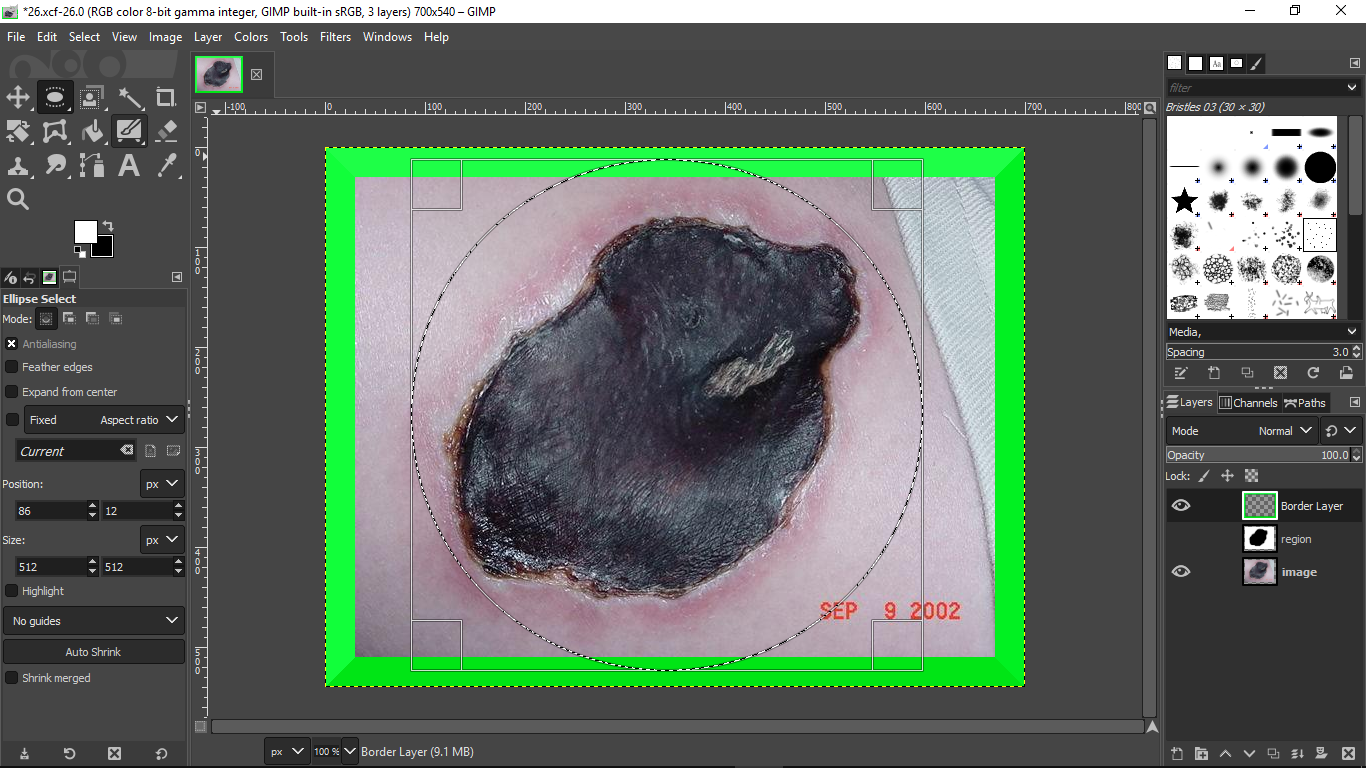
\includegraphics[width=1\textwidth]{gambar/circle_and_border}
	\caption{Citra luka yang telah dicek menggunakan fitur \emph{eclipse select} dan ditambahkan \emph{border}}
	\label{Gambar:circle_and_border}
\end{figure}

Setelah proses \emph{resize} sampai pengecekan lingkaran, selanjutnya penulis \emph{export layer} masing masing ke format .jpg.
\begin{figure}[H]
	\centering
	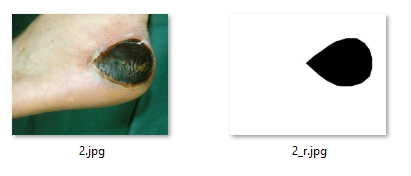
\includegraphics[width=1\textwidth]{gambar/citra_region}
	\caption{Citra luka dan region luka}
	\label{Gambar:citra_region}
\end{figure}




% checkpoint. next olah data di folder my_activecontour

\begin{comment}
\begin{table}[H]
	\centering
	\caption{Rincian data yang akan digunakan kategori luka hitam}
	\label{rinciandataset1}
	\begin{tabular}{|m{1in}|m{1in}|m{1in}|m{1in}|m{1in}|}
		\hline
		\textbf{Citra} & \textbf{\emph{Region}} & \textbf{\emph{Ground truth}} & Kurva awal & Anotasi \\
		\hline
		
		%&  &  & & \\
		%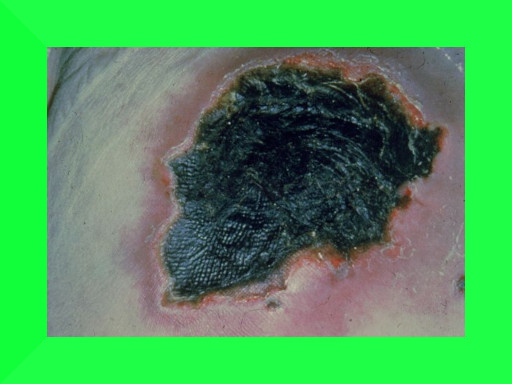
\includegraphics[width=1in]{dataset/dataset_3/luka_hitam/ready/1.jpg} 1.jpg & %
\includegraphics[width=1in]{dataset/dataset_3/luka_hitam/ready/1_r.jpg} 1\_r.jpg & %
\includegraphics[width=1in]{dataset/dataset_3/luka_hitam/ready/1_g.jpg} 1\_g.jpg &
		%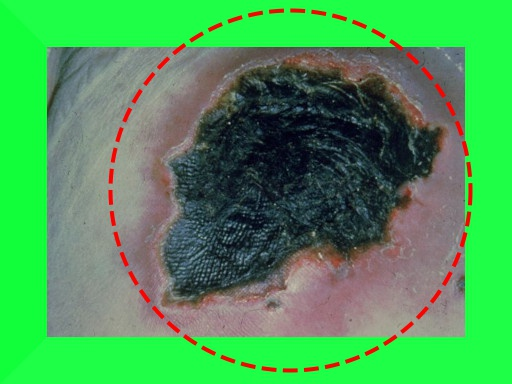
\includegraphics[width=1in]{dataset/dataset_3/luka_hitam/ready/1_init.jpg} 1\_init.jpg &
		%cr=190 
		%cc=290
		%r=180\\
		%\hline
		
		&  &  & & \\
		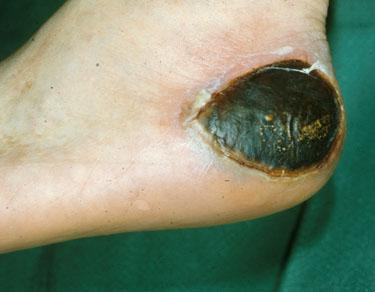
\includegraphics[width=1in]{dataset/dataset_3/luka_hitam/ready/2.jpg} 2.jpg & 
\includegraphics[width=1in]{dataset/dataset_3/luka_hitam/ready/2_r.jpg} 2\_r.jpg & 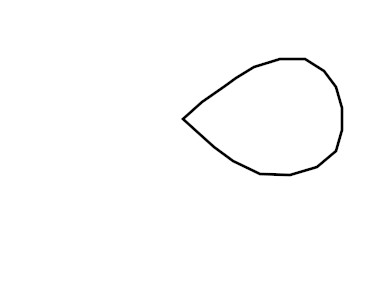
\includegraphics[width=1in]{dataset/dataset_3/luka_hitam/ready/2_g.jpg} 2\_g.jpg &
		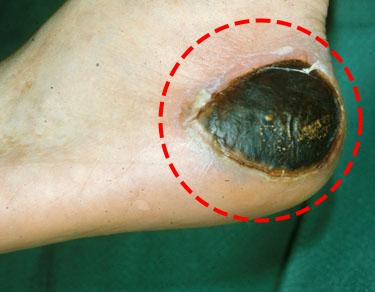
\includegraphics[width=1in]{dataset/dataset_3/luka_hitam/ready/2_init.jpg} 2\_init.jpg &
		cr=120
		cc=265
		r=85\\
		\hline
		
		&  &  & & \\
		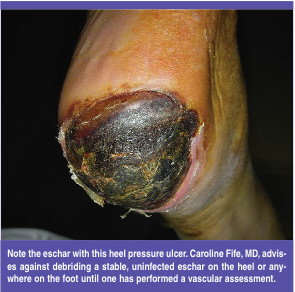
\includegraphics[width=1in]{dataset/dataset_3/luka_hitam/ready/4.jpg} 4.jpg & 
\includegraphics[width=1in]{dataset/dataset_3/luka_hitam/ready/4_r.jpg} 4\_r.jpg & 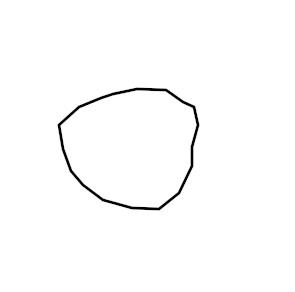
\includegraphics[width=1in]{dataset/dataset_3/luka_hitam/ready/4_g.jpg} 4\_g.jpg &
		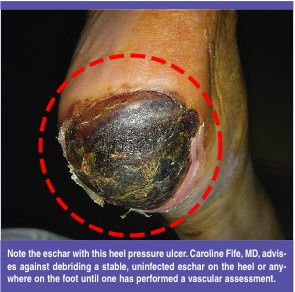
\includegraphics[width=1in]{dataset/dataset_3/luka_hitam/ready/4_init.jpg} 4\_init.jpg &
		cr=145
		cc=130
		r=90\\
		\hline
		
		&  &  & & \\
		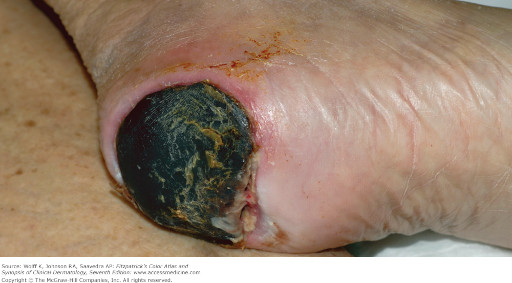
\includegraphics[width=1in]{dataset/dataset_3/luka_hitam/ready/5.jpg} 5.jpg & 
\includegraphics[width=1in]{dataset/dataset_3/luka_hitam/ready/5_r.jpg} 5\_r.jpg & 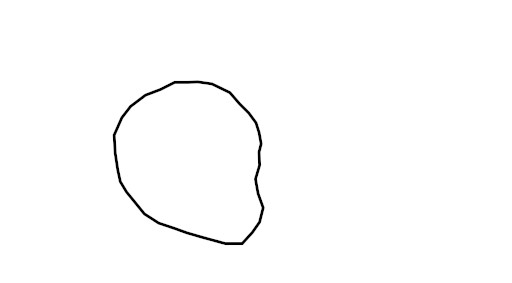
\includegraphics[width=1in]{dataset/dataset_3/luka_hitam/ready/5_g.jpg} 5\_g.jpg &
		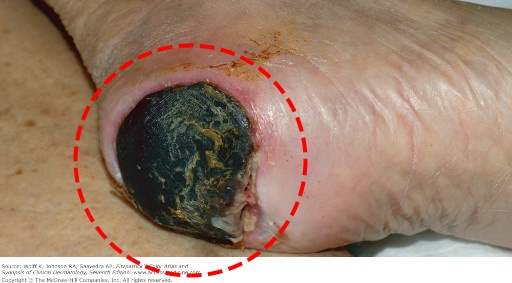
\includegraphics[width=1in]{dataset/dataset_3/luka_hitam/ready/5_init.jpg} 5\_init.jpg &
		cr=160
		cc=190
		r=115\\
		\hline
	\end{tabular}
\end{table}

\begin{table}[H]
	\centering
	\caption{Rincian data yang akan digunakan kategori luka hitam (lanjutan)}
	\label{rinciandataset2}
	\begin{tabular}{|m{1in}|m{1in}|m{1in}|m{1in}|m{1in}|}
		\hline
		\textbf{Citra} & \textbf{\emph{Region}} & \textbf{\emph{Ground truth}} & Kurva awal & Anotasi \\
		\hline
		
		&  &  & & \\
		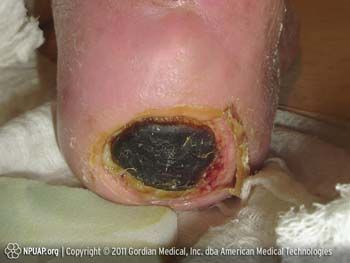
\includegraphics[width=1in]{dataset/dataset_3/luka_hitam/ready/6.jpg} 6.jpg & 
\includegraphics[width=1in]{dataset/dataset_3/luka_hitam/ready/6_r.jpg} 6\_r.jpg & 
\includegraphics[width=1in]{dataset/dataset_3/luka_hitam/ready/6_g.jpg} 6\_g.jpg &
		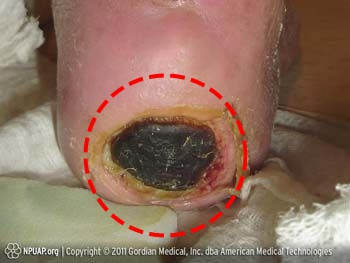
\includegraphics[width=1in]{dataset/dataset_3/luka_hitam/ready/6_init.jpg} 6\_init.jpg &
		cr=155
		cc=165
		r=80\\
		\hline
		
		&  &  & & \\
		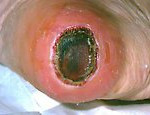
\includegraphics[width=1in]{dataset/dataset_3/luka_hitam/ready/7.jpg} 7.jpg & 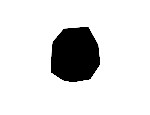
\includegraphics[width=1in]{dataset/dataset_3/luka_hitam/ready/7_r.jpg} 7\_r.jpg & 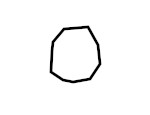
\includegraphics[width=1in]{dataset/dataset_3/luka_hitam/ready/7_g.jpg} 7\_g.jpg &
		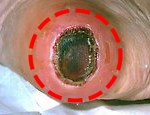
\includegraphics[width=1in]{dataset/dataset_3/luka_hitam/ready/7_init.jpg} 7\_init.jpg &
		cr=55
		cc=75
		r=45\\
		\hline
		
		&  &  & & \\
		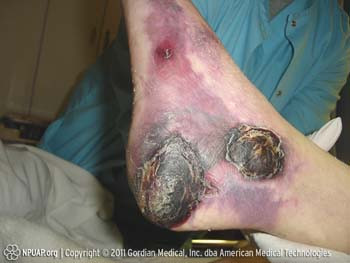
\includegraphics[width=1in]{dataset/dataset_3/luka_hitam/ready/8.jpg} 8.jpg & 
\includegraphics[width=1in]{dataset/dataset_3/luka_hitam/ready/8_r.jpg} 8\_r.jpg & 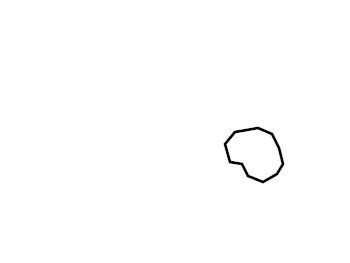
\includegraphics[width=1in]{dataset/dataset_3/luka_hitam/ready/8_g.jpg} 8\_g.jpg &
		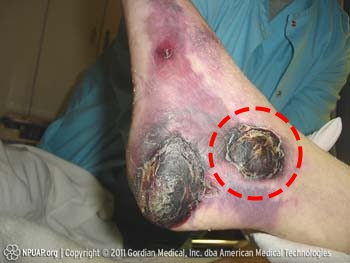
\includegraphics[width=1in]{dataset/dataset_3/luka_hitam/ready/8_init.jpg} 8\_init.jpg &
		cr=153
		cc=255
		r=45\\
		\hline
		
		&  &  & & \\
		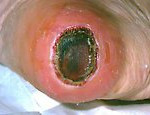
\includegraphics[width=1in]{dataset/dataset_3/luka_hitam/duplicate_or_copyright/9.jpg} 9.jpg & 
\includegraphics[width=1in]{dataset/dataset_3/luka_hitam/duplicate_or_copyright/9_r.jpg} 9\_r.jpg & 
\includegraphics[width=1in]{dataset/dataset_3/luka_hitam/duplicate_or_copyright/9_g.jpg} 9\_g.jpg &
		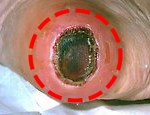
\includegraphics[width=1in]{dataset/dataset_3/luka_hitam/duplicate_or_copyright/9_init.jpg} 9\_init.jpg &
		cr=55
		cc=75
		r=45\\
		\hline
		
		&  &  & & \\
		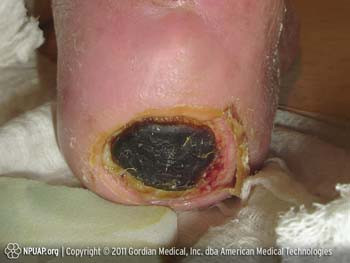
\includegraphics[width=1in]{dataset/dataset_3/luka_hitam/duplicate_or_copyright/11.jpg} 11.jpg & 
\includegraphics[width=1in]{dataset/dataset_3/luka_hitam/duplicate_or_copyright/11_r.jpg} 11\_r.jpg & 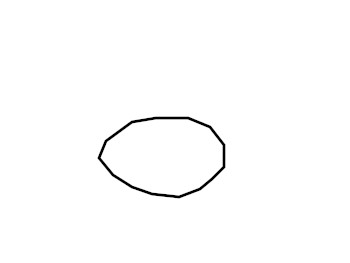
\includegraphics[width=1in]{dataset/dataset_3/luka_hitam/duplicate_or_copyright/11_g.jpg} 11\_g.jpg &
		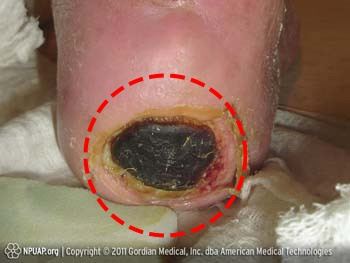
\includegraphics[width=1in]{dataset/dataset_3/luka_hitam/duplicate_or_copyright/11_init.jpg} 11\_init.jpg &
		cr=155
		cc=165
		r=80\\
		\hline
	\end{tabular}
\end{table}

\begin{table}[H]
	\centering
	\caption{Rincian data yang akan digunakan kategori luka hitam (lanjutan)}
	\label{rinciandataset3}
	\begin{tabular}{|m{1in}|m{1in}|m{1in}|m{1in}|m{1in}|}
		\hline
		\textbf{Citra} & \textbf{\emph{Region}} & \textbf{\emph{Ground truth}} & Kurva awal & Anotasi \\
		\hline
		
		&  &  & & \\
		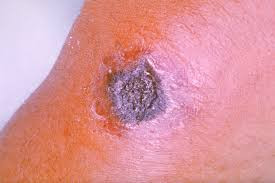
\includegraphics[width=1in]{dataset/dataset_3/luka_hitam/ready/14.jpg} 14.jpg & \includegraphics[width=1in]{dataset/dataset_3/luka_hitam/ready/14_r.jpg} 14\_r.jpg & \includegraphics[width=1in]{dataset/dataset_3/luka_hitam/ready/14_g.jpg} 14\_g.jpg &
		\includegraphics[width=1in]{dataset/dataset_3/luka_hitam/ready/14_init.jpg} 14\_init.jpg &
		cr=95
		cc=130
		r=65\\
		\hline
		
		&  &  & & \\
		\includegraphics[width=1in]{dataset/dataset_3/luka_hitam/ready/15.jpg} 15.jpg & \includegraphics[width=1in]{dataset/dataset_3/luka_hitam/ready/15_r.jpg} 15\_r.jpg & \includegraphics[width=1in]{dataset/dataset_3/luka_hitam/ready/15_g.jpg} 15\_g.jpg &
		\includegraphics[width=1in]{dataset/dataset_3/luka_hitam/ready/15_init.jpg} 15\_init.jpg &
		cr=153
		cc=250
		r=151\\
		\hline
		
		&  &  & & \\
		\includegraphics[width=1in]{dataset/dataset_3/luka_hitam/ready/16.jpg} 16.jpg & \includegraphics[width=1in]{dataset/dataset_3/luka_hitam/ready/16_r.jpg} 16\_r.jpg & \includegraphics[width=1in]{dataset/dataset_3/luka_hitam/ready/16_g.jpg} 16\_g.jpg &
		\includegraphics[width=1in]{dataset/dataset_3/luka_hitam/ready/16_init.jpg} 16\_init.jpg &
		cr=208
		cc=245
		r=200\\
		\hline
		
		&  &  & & \\
		\includegraphics[width=1in]{dataset/dataset_3/luka_hitam/ready/17.jpg} 17.jpg & \includegraphics[width=1in]{dataset/dataset_3/luka_hitam/ready/17_r.jpg} 17\_r.jpg & \includegraphics[width=1in]{dataset/dataset_3/luka_hitam/ready/17_g.jpg} 17\_g.jpg &
		\includegraphics[width=1in]{dataset/dataset_3/luka_hitam/ready/17_init.jpg} 17\_init.jpg &
		cr=124
		cc=125
		r=120\\
		\hline
		
		&  &  & & \\
		\includegraphics[width=1in]{dataset/dataset_3/luka_hitam/ready/18.jpg} 18.jpg & \includegraphics[width=1in]{dataset/dataset_3/luka_hitam/ready/18_r.jpg} 18\_r.jpg & \includegraphics[width=1in]{dataset/dataset_3/luka_hitam/ready/18_g.jpg} 18\_g.jpg &
		\includegraphics[width=1in]{dataset/dataset_3/luka_hitam/ready/18_init.jpg} 18\_init.jpg &
		cr=85
		cc=85
		r=75\\
		\hline
	\end{tabular}
\end{table}

\begin{table}[H]
	\centering
	\caption{Rincian data yang akan digunakan kategori luka hitam (lanjutan)}
	\label{rinciandataset4}
	\begin{tabular}{|m{1in}|m{1in}|m{1in}|m{1in}|m{1in}|}
		\hline
		\textbf{Citra} & \textbf{\emph{Region}} & \textbf{\emph{Ground truth}} & Kurva awal & Anotasi \\
		\hline
		
		&  &  & & \\
		\includegraphics[width=1in]{dataset/dataset_3/luka_hitam/ready/19.jpg} 19.jpg & \includegraphics[width=1in]{dataset/dataset_3/luka_hitam/ready/19_r.jpg} 19\_r.jpg & \includegraphics[width=1in]{dataset/dataset_3/luka_hitam/ready/19_g.jpg} 19\_g.jpg &
		\includegraphics[width=1in]{dataset/dataset_3/luka_hitam/ready/19_init.jpg} 19\_init.jpg &
		cr=225
		cc=285
		r=130\\
		\hline
		
		&  &  & & \\
		\includegraphics[width=1in]{dataset/dataset_3/luka_hitam/ready/20.jpg} 20.jpg & \includegraphics[width=1in]{dataset/dataset_3/luka_hitam/ready/20_r.jpg} 20\_r.jpg & \includegraphics[width=1in]{dataset/dataset_3/luka_hitam/ready/20_g.jpg} 20\_g.jpg &
		\includegraphics[width=1in]{dataset/dataset_3/luka_hitam/ready/20_init.jpg} 20\_init.jpg &
		cr=250
		cc=225
		r=155\\
		\hline
		
		&  &  & & \\
		\includegraphics[width=1in]{dataset/dataset_3/luka_hitam/ready/22.jpg} 22.jpg & \includegraphics[width=1in]{dataset/dataset_3/luka_hitam/ready/22_r.jpg} 22\_r.jpg & \includegraphics[width=1in]{dataset/dataset_3/luka_hitam/ready/22_g.jpg} 22\_g.jpg &
		\includegraphics[width=1in]{dataset/dataset_3/luka_hitam/ready/22_init.jpg} 22\_init.jpg &
		cr=140
		cc=190
		r=125\\
		\hline
		
		&  &  & & \\
		\includegraphics[width=1in]{dataset/dataset_3/luka_hitam/duplicate_or_copyright/24.jpg} 24.jpg & \includegraphics[width=1in]{dataset/dataset_3/luka_hitam/duplicate_or_copyright/24_r.jpg} 24\_r.jpg & \includegraphics[width=1in]{dataset/dataset_3/luka_hitam/duplicate_or_copyright/24_g.jpg} 24\_g.jpg &
		\includegraphics[width=1in]{dataset/dataset_3/luka_hitam/duplicate_or_copyright/24_init.jpg} 24\_init.jpg &
		cr=190
		cc=190
		r=180\\
		\hline
		
		&  &  & & \\
		\includegraphics[width=1in]{dataset/dataset_3/luka_hitam/ready/26.jpg} 26.jpg & \includegraphics[width=1in]{dataset/dataset_3/luka_hitam/ready/26_r.jpg} 26\_r.jpg & \includegraphics[width=1in]{dataset/dataset_3/luka_hitam/ready/26_g.jpg} 26\_g.jpg &
		\includegraphics[width=1in]{dataset/dataset_3/luka_hitam/ready/26_init.jpg} 26\_init.jpg &
		cr=195
		cc=248
		r=193\\
		\hline
	\end{tabular}
\end{table}

\begin{table}[H]
	\centering
	\caption{Rincian data yang akan digunakan kategori luka hitam (lanjutan)}
	\label{rinciandataset5}
	\begin{tabular}{|m{1in}|m{1in}|m{1in}|m{1in}|m{1in}|}
		\hline
		\textbf{Citra} & \textbf{\emph{Region}} & \textbf{\emph{Ground truth}} & Kurva awal & Anotasi \\
		\hline
		
		&  &  & & \\
		\includegraphics[width=1in]{dataset/dataset_3/luka_hitam/ready/27.jpg} 27.jpg & \includegraphics[width=1in]{dataset/dataset_3/luka_hitam/ready/27_r.jpg} 27\_r.jpg & \includegraphics[width=1in]{dataset/dataset_3/luka_hitam/ready/27_g.jpg} 27\_g.jpg &
		\includegraphics[width=1in]{dataset/dataset_3/luka_hitam/ready/27_init.jpg} 27\_init.jpg &
		cr=207
		cc=253
		r=205\\
		\hline
		
		&  &  & & \\
		\includegraphics[width=1in]{dataset/dataset_3/luka_hitam/ready/28.jpg} 28.jpg & \includegraphics[width=1in]{dataset/dataset_3/luka_hitam/ready/28_r.jpg} 28\_r.jpg & \includegraphics[width=1in]{dataset/dataset_3/luka_hitam/ready/28_g.jpg} 28\_g.jpg &
		\includegraphics[width=1in]{dataset/dataset_3/luka_hitam/ready/28_init.jpg} 28\_init.jpg &
		cr=120
		cc=80
		r=70\\
		\hline
		
		&  &  & & \\
		\includegraphics[width=1in]{dataset/dataset_3/luka_hitam/ready/29.jpg} 29.jpg & \includegraphics[width=1in]{dataset/dataset_3/luka_hitam/ready/29_r.jpg} 29\_r.jpg & \includegraphics[width=1in]{dataset/dataset_3/luka_hitam/ready/29_g.jpg} 29\_g.jpg &
		\includegraphics[width=1in]{dataset/dataset_3/luka_hitam/ready/16_init.jpg} 29\_init.jpg &
		cr=195
		cc=240
		r=180\\
		\hline
		
		&  &  & & \\
		\includegraphics[width=1in]{dataset/dataset_3/luka_hitam/ready/31.jpg} 31.jpg & \includegraphics[width=1in]{dataset/dataset_3/luka_hitam/ready/31_r.jpg} 31\_r.jpg & \includegraphics[width=1in]{dataset/dataset_3/luka_hitam/ready/31_g.jpg} 31\_g.jpg &
		\includegraphics[width=1in]{dataset/dataset_3/luka_hitam/ready/31_init.jpg} 31\_init.jpg &
		cr=245
		cc=190
		r=180\\
		\hline
		
		&  &  & & \\
		\includegraphics[width=1in]{dataset/dataset_3/luka_hitam/ready/33.jpg} 33.jpg & \includegraphics[width=1in]{dataset/dataset_3/luka_hitam/ready/33_r.jpg} 33\_r.jpg & \includegraphics[width=1in]{dataset/dataset_3/luka_hitam/ready/33_g.jpg} 33\_g.jpg &
		\includegraphics[width=1in]{dataset/dataset_3/luka_hitam/ready/33_init.jpg} 33\_init.jpg &
		cr=120
		cc=195
		r=100\\
		\hline
	\end{tabular}
\end{table}

\begin{table}[H]
	\centering
	\caption{Rincian data yang akan digunakan kategori luka hitam (lanjutan)}
	\label{rinciandataset6}
	\begin{tabular}{|m{1in}|m{1in}|m{1in}|m{1in}|m{1in}|}
		\hline
		\textbf{Citra} & \textbf{\emph{Region}} & \textbf{\emph{Ground truth}} & Kurva awal & Anotasi \\
		\hline
		
		&  &  & & \\
		\includegraphics[width=1in]{dataset/dataset_3/luka_hitam/ready/37.jpg} 37.jpg & \includegraphics[width=1in]{dataset/dataset_3/luka_hitam/ready/37_r.jpg} 37\_r.jpg & \includegraphics[width=1in]{dataset/dataset_3/luka_hitam/ready/37_g.jpg} 37\_g.jpg &
		\includegraphics[width=1in]{dataset/dataset_3/luka_hitam/ready/37_init.jpg} 37\_init.jpg &
		cr=110
		cc=125
		r=95\\
		\hline
		
		&  &  & & \\
		\includegraphics[width=1in]{dataset/dataset_3/luka_hitam/ready/39.jpg} 39.jpg & \includegraphics[width=1in]{dataset/dataset_3/luka_hitam/ready/39_r.jpg} 39\_r.jpg & \includegraphics[width=1in]{dataset/dataset_3/luka_hitam/ready/39_g.jpg} 39\_g.jpg &
		\includegraphics[width=1in]{dataset/dataset_3/luka_hitam/ready/39_init.jpg} 39\_init.jpg &
		cr=260
		cc=265
		r=170\\
		\hline
		
		&  &  & & \\
		\includegraphics[width=1in]{dataset/dataset_3/luka_hitam/ready/40.jpg} 40.jpg & \includegraphics[width=1in]{dataset/dataset_3/luka_hitam/ready/40_r.jpg} 40\_r.jpg & \includegraphics[width=1in]{dataset/dataset_3/luka_hitam/ready/40_g.jpg} 40\_g.jpg &
		\includegraphics[width=1in]{dataset/dataset_3/luka_hitam/ready/40_init.jpg} 40\_init.jpg &
		cr=90
		cc=100
		r=65\\
		\hline
		
		&  &  & & \\
		\includegraphics[width=1in]{dataset/dataset_3/luka_hitam/ready/41.jpg} 41.jpg & \includegraphics[width=1in]{dataset/dataset_3/luka_hitam/ready/41_r.jpg} 41\_r.jpg & \includegraphics[width=1in]{dataset/dataset_3/luka_hitam/ready/41_g.jpg} 41\_g.jpg &
		\includegraphics[width=1in]{dataset/dataset_3/luka_hitam/ready/41_init.jpg} 41\_init.jpg &
		cr=105
		cc=170
		r=100\\
		\hline
	\end{tabular}
\end{table}


\begin{table}[H]
	\centering
	\caption{Rincian data yang akan digunakan kategori luka kuning}
	\label{rinciandataset7}
	\begin{tabular}{|m{1in}|m{1in}|m{1in}|m{1in}|m{1in}|}
		\hline
		\textbf{Citra} & \textbf{\emph{Region}} & \textbf{\emph{Ground truth}} & Kurva awal & Anotasi \\
		\hline
		
		&  &  & & \\
		\includegraphics[width=1in]{dataset/dataset_3/luka_kuning/ready/3.jpg} 3.jpg & \includegraphics[width=1in]{dataset/dataset_3/luka_kuning/ready/3_r.jpg} 3\_r.jpg & \includegraphics[width=1in]{dataset/dataset_3/luka_kuning/ready/3_g.jpg} 3\_g.jpg &
		\includegraphics[width=1in]{dataset/dataset_3/luka_kuning/ready/3_init.jpg} 3\_init.jpg &
		cr=80
		cc=85
		r=65\\
		\hline
		
		&  &  & & \\
		\includegraphics[width=1in]{dataset/dataset_3/luka_kuning/ready/10.jpg} 10.jpg & \includegraphics[width=1in]{dataset/dataset_3/luka_kuning/ready/10_r.jpg} 10\_r.jpg & \includegraphics[width=1in]{dataset/dataset_3/luka_kuning/ready/10_g.jpg} 10\_g.jpg &
		\includegraphics[width=1in]{dataset/dataset_3/luka_kuning/ready/10_init.jpg} 10\_init.jpg &
		cr=155
		cc=133
		r=128\\
		\hline
		
		&  &  & & \\
		\includegraphics[width=1in]{dataset/dataset_3/luka_kuning/ready/12.jpg} 12.jpg & \includegraphics[width=1in]{dataset/dataset_3/luka_kuning/ready/12_r.jpg} 12\_r.jpg & \includegraphics[width=1in]{dataset/dataset_3/luka_kuning/ready/12_g.jpg} 12\_g.jpg &
		\includegraphics[width=1in]{dataset/dataset_3/luka_kuning/ready/12_init.jpg} 12\_init.jpg &
		cr=90
		cc=138
		r=70\\
		\hline
		
		&  &  & & \\
		\includegraphics[width=1in]{dataset/dataset_3/luka_kuning/ready/13.jpg} 13.jpg & \includegraphics[width=1in]{dataset/dataset_3/luka_kuning/ready/13_r.jpg} 13\_r.jpg & \includegraphics[width=1in]{dataset/dataset_3/luka_kuning/ready/13_g.jpg} 13\_g.jpg &
		\includegraphics[width=1in]{dataset/dataset_3/luka_kuning/ready/13_init.jpg} 13\_init.jpg &
		cr=70
		cc=206
		r=50\\
		\hline
		
		&  &  & & \\
		\includegraphics[width=1in]{dataset/dataset_3/luka_kuning/ready/16.jpg} 16.jpg & \includegraphics[width=1in]{dataset/dataset_3/luka_kuning/ready/16_r.jpg} 16\_r.jpg & \includegraphics[width=1in]{dataset/dataset_3/luka_kuning/ready/16_g.jpg} 16\_g.jpg &
		\includegraphics[width=1in]{dataset/dataset_3/luka_kuning/ready/16_init.jpg} 16\_init.jpg &
		cr=135
		cc=172
		r=130\\
		\hline
	\end{tabular}
\end{table}

\begin{table}[H]
	\centering
	\caption{Rincian data yang akan digunakan kategori luka kuning (lanjutan)}
	\label{rinciandataset8}
	\begin{tabular}{|m{1in}|m{1in}|m{1in}|m{1in}|m{1in}|}
		\hline
		\textbf{Citra} & \textbf{\emph{Region}} & \textbf{\emph{Ground truth}} & Kurva awal & Anotasi \\
		\hline
		
		&  &  & & \\
		\includegraphics[width=1in]{dataset/dataset_3/luka_kuning/ready/17.jpg} 17.jpg & \includegraphics[width=1in]{dataset/dataset_3/luka_kuning/ready/17_r.jpg} 17\_r.jpg & \includegraphics[width=1in]{dataset/dataset_3/luka_kuning/ready/17_g.jpg} 17\_g.jpg &
		\includegraphics[width=1in]{dataset/dataset_3/luka_kuning/ready/17_init.jpg} 17\_init.jpg &
		cr=125
		cc=115
		r=25\\
		\hline
		
		&  &  & & \\
		\includegraphics[width=1in]{dataset/dataset_3/luka_kuning/ready/18.jpg} 18.jpg & \includegraphics[width=1in]{dataset/dataset_3/luka_kuning/ready/18_r.jpg} 18\_r.jpg & \includegraphics[width=1in]{dataset/dataset_3/luka_kuning/ready/18_g.jpg} 18\_g.jpg &
		\includegraphics[width=1in]{dataset/dataset_3/luka_kuning/ready/18_init.jpg} 18\_init.jpg &
		cr=95
		cc=130
		r=80\\
		\hline
		
		&  &  & & \\
		\includegraphics[width=1in]{dataset/dataset_3/luka_kuning/ready/19.jpg} 19.jpg & \includegraphics[width=1in]{dataset/dataset_3/luka_kuning/ready/19_r.jpg} 19\_r.jpg & \includegraphics[width=1in]{dataset/dataset_3/luka_kuning/ready/19_g.jpg} 19\_g.jpg &
		\includegraphics[width=1in]{dataset/dataset_3/luka_kuning/ready/19_init.jpg} 19\_init.jpg &
		cr=60
		cc=60
		r=50\\
		\hline
		
		&  &  & & \\
		\includegraphics[width=1in]{dataset/dataset_3/luka_kuning/ready/21.jpg} 21.jpg & \includegraphics[width=1in]{dataset/dataset_3/luka_kuning/ready/21_r.jpg} 21\_r.jpg & \includegraphics[width=1in]{dataset/dataset_3/luka_kuning/ready/21_g.jpg} 21\_g.jpg &
		\includegraphics[width=1in]{dataset/dataset_3/luka_kuning/ready/21_init.jpg} 21\_init.jpg &
		cr=130
		cc=170
		r=70\\
		\hline
		
		&  &  & & \\
		\includegraphics[width=1in]{dataset/dataset_3/luka_kuning/ready/23.jpg} 23.jpg & \includegraphics[width=1in]{dataset/dataset_3/luka_kuning/ready/23_r.jpg} 23\_r.jpg & \includegraphics[width=1in]{dataset/dataset_3/luka_kuning/ready/23_g.jpg} 23\_g.jpg &
		\includegraphics[width=1in]{dataset/dataset_3/luka_kuning/ready/23_init.jpg} 23\_init.jpg &
		cr=170
		cc=230
		r=160\\
		\hline
	\end{tabular}
\end{table}

\begin{table}[H]
	\centering
	\caption{Rincian data yang akan digunakan kategori luka kuning (lanjutan)}
	\label{rinciandataset9}
	\begin{tabular}{|m{1in}|m{1in}|m{1in}|m{1in}|m{1in}|}
		\hline
		\textbf{Citra} & \textbf{\emph{Region}} & \textbf{\emph{Ground truth}} & Kurva awal & Anotasi \\
		\hline
		
		&  &  & & \\
		\includegraphics[width=1in]{dataset/dataset_3/luka_kuning/ready/25.jpg} 25.jpg & \includegraphics[width=1in]{dataset/dataset_3/luka_kuning/ready/25_r.jpg} 25\_r.jpg & \includegraphics[width=1in]{dataset/dataset_3/luka_kuning/ready/25_g.jpg} 25\_g.jpg &
		\includegraphics[width=1in]{dataset/dataset_3/luka_kuning/ready/25_init.jpg} 25\_init.jpg &
		cr=145
		cc=130
		r=55\\
		\hline
		
		&  &  & & \\
		\includegraphics[width=1in]{dataset/dataset_3/luka_kuning/ready/34.jpg} 34.jpg & \includegraphics[width=1in]{dataset/dataset_3/luka_kuning/ready/34_r.jpg} 34\_r.jpg & \includegraphics[width=1in]{dataset/dataset_3/luka_kuning/ready/34_g.jpg} 34\_g.jpg &
		\includegraphics[width=1in]{dataset/dataset_3/luka_kuning/ready/34_init.jpg} 34\_init.jpg &
		cr=185
		cc=245
		r=130\\
		\hline
		
		&  &  & & \\
		\includegraphics[width=1in]{dataset/dataset_3/luka_kuning/ready/35.jpg} 35.jpg & \includegraphics[width=1in]{dataset/dataset_3/luka_kuning/ready/35_r.jpg} 35\_r.jpg & \includegraphics[width=1in]{dataset/dataset_3/luka_kuning/ready/35_g.jpg} 35\_g.jpg &
		\includegraphics[width=1in]{dataset/dataset_3/luka_kuning/ready/35_init.jpg} 35\_init.jpg &
		cr=105
		cc=110
		r=100\\
		\hline
		
		&  &  & & \\
		\includegraphics[width=1in]{dataset/dataset_3/luka_kuning/ready/38.jpg} 38.jpg & \includegraphics[width=1in]{dataset/dataset_3/luka_kuning/ready/38_r.jpg} 38\_r.jpg & \includegraphics[width=1in]{dataset/dataset_3/luka_kuning/ready/38_g.jpg} 38\_g.jpg &
		\includegraphics[width=1in]{dataset/dataset_3/luka_kuning/ready/38_init.jpg} 38\_init.jpg &
		cr=150
		cc=280
		r=120\\
		\hline
		
		&  &  & & \\
		\includegraphics[width=1in]{dataset/dataset_3/luka_kuning/ready/42.jpg} 42.jpg & \includegraphics[width=1in]{dataset/dataset_3/luka_kuning/ready/42_r.jpg} 42\_r.jpg & \includegraphics[width=1in]{dataset/dataset_3/luka_kuning/ready/42_g.jpg} 42\_g.jpg &
		\includegraphics[width=1in]{dataset/dataset_3/luka_kuning/ready/42_init.jpg} 42\_init.jpg &
		cr=160
		cc=260
		r=1135\\
		\hline
	\end{tabular}
\end{table}


\begin{table}[H]
	\centering
	\caption{Rincian data yang akan digunakan kategori luka merah }
	\label{rinciandataset10}
	\begin{tabular}{|m{1in}|m{1in}|m{1in}|m{1in}|m{1in}|}
		\hline
		\textbf{Citra} & \textbf{\emph{Region}} & \textbf{\emph{Ground truth}} & Kurva awal & Anotasi \\
		\hline
		
		&  &  & & \\
		\includegraphics[width=0.8in]{dataset/dataset_3/luka_merah/ready/1.jpg} 1.jpg & \includegraphics[width=0.8in]{dataset/dataset_3/luka_merah/ready/1_r.jpg} 1\_r.jpg & \includegraphics[width=0.8in]{dataset/dataset_3/luka_merah/ready/1_g.jpg} 1\_g.jpg &
		\includegraphics[width=0.8in]{dataset/dataset_3/luka_merah/ready/1_init.jpg} 1\_init.jpg &
		cr=200
		cc=235
		r=190\\
		\hline
		
		&  &  & & \\
		\includegraphics[width=0.8in]{dataset/dataset_3/luka_merah/ready/2.jpg} 2.jpg & \includegraphics[width=0.8in]{dataset/dataset_3/luka_merah/ready/2_r.jpg} 2\_r.jpg & \includegraphics[width=0.8in]{dataset/dataset_3/luka_merah/ready/2_g.jpg} 2\_g.jpg &
		\includegraphics[width=0.8in]{dataset/dataset_3/luka_merah/ready/2_init.jpg} 2\_init.jpg &
		cr=270
		cc=105
		r=100\\
		\hline
		
		&  &  & & \\
		\includegraphics[width=0.8in]{dataset/dataset_3/luka_merah/ready/3.jpg} 3.jpg & \includegraphics[width=0.8in]{dataset/dataset_3/luka_merah/ready/3_r.jpg} 3\_r.jpg & \includegraphics[width=0.8in]{dataset/dataset_3/luka_merah/ready/3_g.jpg} 3\_g.jpg &
		\includegraphics[width=0.8in]{dataset/dataset_3/luka_merah/ready/3_init.jpg} 3\_init.jpg &
		cr=255
		cc=170
		r=100\\
		\hline
		
		&  &  & & \\
		\includegraphics[width=0.8in]{dataset/dataset_3/luka_merah/ready/4.jpg} 4.jpg & \includegraphics[width=0.8in]{dataset/dataset_3/luka_merah/ready/4_r.jpg} 4\_r.jpg & \includegraphics[width=0.8in]{dataset/dataset_3/luka_merah/ready/4_g.jpg} 4\_g.jpg &
		\includegraphics[width=0.8in]{dataset/dataset_3/luka_merah/ready/4_init.jpg} 4\_init.jpg &
		cr=310
		cc=170
		r=150\\
		\hline
		
		&  &  & & \\
		\includegraphics[width=0.8in]{dataset/dataset_3/luka_merah/ready/6.jpg} 6.jpg & \includegraphics[width=0.8in]{dataset/dataset_3/luka_merah/ready/6_r.jpg} 6\_r.jpg & \includegraphics[width=0.8in]{dataset/dataset_3/luka_merah/ready/6_g.jpg} 6\_g.jpg &
		\includegraphics[width=0.8in]{dataset/dataset_3/luka_merah/ready/6_init.jpg} 6\_init.jpg &
		cr=160
		cc=250
		r=120\\
		\hline
	\end{tabular}
\end{table}

\begin{table}[H]
	\centering
	\caption{Rincian data yang akan digunakan kategori luka merah (lanjutan)}
	\label{rinciandataset11}
	\begin{tabular}{|m{1in}|m{1in}|m{1in}|m{1in}|m{1in}|}
		\hline
		\textbf{Citra} & \textbf{\emph{Region}} & \textbf{\emph{Ground truth}} & Kurva awal & Anotasi \\
		\hline
		
		&  &  & & \\
		\includegraphics[width=1in]{dataset/dataset_3/luka_merah/ready/7.jpg} 7.jpg & \includegraphics[width=1in]{dataset/dataset_3/luka_merah/ready/7_r.jpg} 7\_r.jpg & \includegraphics[width=1in]{dataset/dataset_3/luka_merah/ready/7_g.jpg} 7\_g.jpg &
		\includegraphics[width=1in]{dataset/dataset_3/luka_merah/ready/7_init.jpg} 7\_init.jpg &
		cr=180
		cc=250
		r=90\\
		\hline
		
		&  &  & & \\
		\includegraphics[width=1in]{dataset/dataset_3/luka_merah/ready/8.jpg} 8.jpg & \includegraphics[width=1in]{dataset/dataset_3/luka_merah/ready/8_r.jpg} 8\_r.jpg & \includegraphics[width=1in]{dataset/dataset_3/luka_merah/ready/8_g.jpg} 8\_g.jpg &
		\includegraphics[width=1in]{dataset/dataset_3/luka_merah/ready/8_init.jpg} 8\_init.jpg &
		cr=220
		cc=260
		r=140\\
		\hline
		
		&  &  & & \\
		\includegraphics[width=1in]{dataset/dataset_3/luka_merah/ready/9.jpg} 9.jpg & \includegraphics[width=1in]{dataset/dataset_3/luka_merah/ready/9_r.jpg} 9\_r.jpg & \includegraphics[width=1in]{dataset/dataset_3/luka_merah/ready/9_g.jpg} 9\_g.jpg &
		\includegraphics[width=1in]{dataset/dataset_3/luka_merah/ready/9_init.jpg} 9\_init.jpg &
		cr=236
		cc=130
		r=70\\
		\hline
		
		&  &  & & \\
		\includegraphics[width=1in]{dataset/dataset_3/luka_merah/ready/10.jpg} 10.jpg & \includegraphics[width=1in]{dataset/dataset_3/luka_merah/ready/10_r.jpg} 10\_r.jpg & \includegraphics[width=1in]{dataset/dataset_3/luka_merah/ready/10_g.jpg} 10\_g.jpg &
		\includegraphics[width=1in]{dataset/dataset_3/luka_merah/ready/10_init.jpg} 10\_init.jpg &
		cr=180
		cc=240
		r=90\\
		\hline
		
		&  &  & & \\
		\includegraphics[width=1in]{dataset/dataset_3/luka_merah/ready/11.jpg} 11.jpg & \includegraphics[width=1in]{dataset/dataset_3/luka_merah/ready/11_r.jpg} 11\_r.jpg & \includegraphics[width=1in]{dataset/dataset_3/luka_merah/ready/11_g.jpg} 11\_g.jpg &
		\includegraphics[width=1in]{dataset/dataset_3/luka_merah/ready/11_init.jpg} 11\_init.jpg &
		cr=190
		cc=295
		r=170\\
		\hline
	\end{tabular}
\end{table}

\begin{table}[H]
	\centering
	\caption{Rincian data yang akan digunakan kategori luka merah (lanjutan)}
	\label{rinciandataset12}
	\begin{tabular}{|m{1in}|m{1in}|m{1in}|m{1in}|m{1in}|}
		\hline
		\textbf{Citra} & \textbf{\emph{Region}} & \textbf{\emph{Ground truth}} & Kurva awal & Anotasi \\
		\hline
		
		&  &  & & \\
		\includegraphics[width=1in]{dataset/dataset_3/luka_merah/ready/12.jpg} 12.jpg & \includegraphics[width=1in]{dataset/dataset_3/luka_merah/ready/12_r.jpg} 12\_r.jpg & \includegraphics[width=1in]{dataset/dataset_3/luka_merah/ready/12_g.jpg} 12\_g.jpg &
		\includegraphics[width=1in]{dataset/dataset_3/luka_merah/ready/12_init.jpg} 12\_init.jpg &
		cr=200
		cc=245
		r=155\\
		\hline
		
		&  &  & & \\
		\includegraphics[width=1in]{dataset/dataset_3/luka_merah/ready/14.jpg} 14.jpg & \includegraphics[width=1in]{dataset/dataset_3/luka_merah/ready/14_r.jpg} 14\_r.jpg & \includegraphics[width=1in]{dataset/dataset_3/luka_merah/ready/14_g.jpg} 14\_g.jpg &
		\includegraphics[width=1in]{dataset/dataset_3/luka_merah/ready/14_init.jpg} 14\_init.jpg &
		cr=180
		cc=263
		r=175\\
		\hline
		
		&  &  & & \\
		\includegraphics[width=1in]{dataset/dataset_3/luka_merah/ready/16.jpg} 16.jpg & \includegraphics[width=1in]{dataset/dataset_3/luka_merah/ready/16_r.jpg} 16\_r.jpg & \includegraphics[width=1in]{dataset/dataset_3/luka_merah/ready/16_g.jpg} 16\_g.jpg &
		\includegraphics[width=1in]{dataset/dataset_3/luka_merah/ready/16_init.jpg} 16\_init.jpg &
		cr=105
		cc=140
		r=90\\
		\hline
		
		&  &  & & \\
		\includegraphics[width=1in]{dataset/dataset_3/luka_merah/ready/17.jpg} 17.jpg & \includegraphics[width=1in]{dataset/dataset_3/luka_merah/ready/17_r.jpg} 17\_r.jpg & \includegraphics[width=1in]{dataset/dataset_3/luka_merah/ready/17_g.jpg} 17\_g.jpg &
		\includegraphics[width=1in]{dataset/dataset_3/luka_merah/ready/17_init.jpg} 17\_init.jpg &
		cr=105
		cc=160
		r=90\\
		\hline
		
		&  &  & & \\
		\includegraphics[width=1in]{dataset/dataset_3/luka_merah/ready/18.jpg} 18.jpg & \includegraphics[width=1in]{dataset/dataset_3/luka_merah/ready/18_r.jpg} 18\_r.jpg & \includegraphics[width=1in]{dataset/dataset_3/luka_merah/ready/18_g.jpg} 18\_g.jpg &
		\includegraphics[width=1in]{dataset/dataset_3/luka_merah/ready/18_init.jpg} 18\_init.jpg &
		cr=180
		cc=280
		r=70\\
		\hline
	\end{tabular}
\end{table}

\begin{table}[H]
	\centering
	\caption{Rincian data yang akan digunakan kategori luka merah (lanjutan) }
	\label{rinciandataset13}
	\begin{tabular}{|m{1in}|m{1in}|m{1in}|m{1in}|m{1in}|}
		\hline
		\textbf{Citra} & \textbf{\emph{Region}} & \textbf{\emph{Ground truth}} & Kurva awal & Anotasi \\
		\hline
		
		&  &  & & \\
		\includegraphics[width=1in]{dataset/dataset_3/luka_merah/ready/19.jpg} 19.jpg & \includegraphics[width=1in]{dataset/dataset_3/luka_merah/ready/19_r.jpg} 19\_r.jpg & \includegraphics[width=1in]{dataset/dataset_3/luka_merah/ready/19_g.jpg} 19\_g.jpg &
		\includegraphics[width=1in]{dataset/dataset_3/luka_merah/ready/19_init.jpg} 19\_init.jpg &
		cr=215
		cc=275
		r=215\\
		\hline
		
		&  &  & & \\
		\includegraphics[width=1in]{dataset/dataset_3/luka_merah/ready/20.jpg} 20.jpg & \includegraphics[width=1in]{dataset/dataset_3/luka_merah/ready/20_r.jpg} 20\_r.jpg & \includegraphics[width=1in]{dataset/dataset_3/luka_merah/ready/20_g.jpg} 20\_g.jpg &
		\includegraphics[width=1in]{dataset/dataset_3/luka_merah/ready/20_init.jpg} 20\_init.jpg &
		cr=180
		cc=204
		r=173\\
		\hline
		
		&  &  & & \\
		\includegraphics[width=1in]{dataset/dataset_3/luka_merah/ready/22.jpg} 22.jpg & \includegraphics[width=1in]{dataset/dataset_3/luka_merah/ready/22_r.jpg} 22\_r.jpg & \includegraphics[width=1in]{dataset/dataset_3/luka_merah/ready/22_g.jpg} 22\_g.jpg &
		\includegraphics[width=1in]{dataset/dataset_3/luka_merah/ready/22_init.jpg} 22\_init.jpg &
		cr=180
		cc=225
		r=150\\
		\hline
		
		&  &  & & \\
		\includegraphics[width=1in]{dataset/dataset_3/luka_merah/ready/23.jpg} 23.jpg & \includegraphics[width=1in]{dataset/dataset_3/luka_merah/ready/23_r.jpg} 23\_r.jpg & \includegraphics[width=1in]{dataset/dataset_3/luka_merah/ready/23_g.jpg} 23\_g.jpg &
		\includegraphics[width=1in]{dataset/dataset_3/luka_merah/ready/23_init.jpg} 23\_init.jpg &
		cr=200
		cc=235
		r=190\\
		\hline
		
		&  &  & & \\
		\includegraphics[width=1in]{dataset/dataset_3/luka_merah/ready/24.jpg} 24.jpg & \includegraphics[width=1in]{dataset/dataset_3/luka_merah/ready/24_r.jpg} 24\_r.jpg & \includegraphics[width=1in]{dataset/dataset_3/luka_merah/ready/24_g.jpg} 24\_g.jpg &
		\includegraphics[width=1in]{dataset/dataset_3/luka_merah/ready/24_init.jpg} 24\_init.jpg &
		cr=150
		cc=150
		r=145\\
		\hline
	\end{tabular}
\end{table}

\begin{table}[H]
	\centering
	\caption{Rincian data yang akan digunakan kategori luka merah (lanjutan) }
	\label{rinciandataset14}
	\begin{tabular}{|m{1in}|m{1in}|m{1in}|m{1in}|m{1in}|}
		\hline
		\textbf{Citra} & \textbf{\emph{Region}} & \textbf{\emph{Ground truth}} & Kurva awal & Anotasi \\
		\hline
		
		&  &  & & \\
		\includegraphics[width=1in]{dataset/dataset_3/luka_merah/ready/25.jpg} 25.jpg & \includegraphics[width=1in]{dataset/dataset_3/luka_merah/ready/25_r.jpg} 25\_r.jpg & \includegraphics[width=1in]{dataset/dataset_3/luka_merah/ready/25_g.jpg} 25\_g.jpg &
		\includegraphics[width=1in]{dataset/dataset_3/luka_merah/ready/25_init.jpg} 25\_init.jpg &
		cr=240
		cc=320
		r=135\\
		\hline
		
		&  &  & & \\
		\includegraphics[width=1in]{dataset/dataset_3/luka_merah/ready/26.jpg} 26.jpg & \includegraphics[width=1in]{dataset/dataset_3/luka_merah/ready/26_r.jpg} 26\_r.jpg & \includegraphics[width=1in]{dataset/dataset_3/luka_merah/ready/26_g.jpg} 26\_g.jpg &
		\includegraphics[width=1in]{dataset/dataset_3/luka_merah/ready/26_init.jpg} 26\_init.jpg &
		cr=230
		cc=280
		r=225\\
		\hline
		
		&  &  & & \\
		\includegraphics[width=1in]{dataset/dataset_3/luka_merah/ready/29.jpg} 29.jpg & \includegraphics[width=1in]{dataset/dataset_3/luka_merah/ready/29_r.jpg} 29\_r.jpg & \includegraphics[width=1in]{dataset/dataset_3/luka_merah/ready/29_g.jpg} 29\_g.jpg &
		\includegraphics[width=1in]{dataset/dataset_3/luka_merah/ready/29_init.jpg} 29\_init.jpg &
		cr=105
		cc=160
		r=90\\
		\hline
		
		&  &  & & \\
		\includegraphics[width=1in]{dataset/dataset_3/luka_merah/ready/30.jpg} 30.jpg & \includegraphics[width=1in]{dataset/dataset_3/luka_merah/ready/30_r.jpg} 30\_r.jpg & \includegraphics[width=1in]{dataset/dataset_3/luka_merah/ready/30_g.jpg} 30\_g.jpg &
		\includegraphics[width=1in]{dataset/dataset_3/luka_merah/ready/30_init.jpg} 30\_init.jpg &
		cr=200
		cc=235
		r=190\\
		\hline
		
		&  &  & & \\
		\includegraphics[width=1in]{dataset/dataset_3/luka_merah/ready/31.jpg} 31.jpg & \includegraphics[width=1in]{dataset/dataset_3/luka_merah/ready/31_r.jpg} 31\_r.jpg & \includegraphics[width=1in]{dataset/dataset_3/luka_merah/ready/31_g.jpg} 31\_g.jpg &
		\includegraphics[width=1in]{dataset/dataset_3/luka_merah/ready/31_init.jpg} 31\_init.jpg &
		cr=120
		cc=185
		r=90\\
		\hline
	\end{tabular}
\end{table}

\begin{table}[H]
	\centering
	\caption{Rincian data yang akan digunakan kategori luka merah (lanjutan) }
	\label{rinciandataset15}
	\begin{tabular}{|m{1in}|m{1in}|m{1in}|m{1in}|m{1in}|}
		\hline
		\textbf{Citra} & \textbf{\emph{Region}} & \textbf{\emph{Ground truth}} & Kurva awal & Anotasi \\
		\hline
		
		&  &  & & \\
		\includegraphics[width=1in]{dataset/dataset_3/luka_merah/ready/32.jpg} 32.jpg & \includegraphics[width=1in]{dataset/dataset_3/luka_merah/ready/32_r.jpg} 32\_r.jpg & \includegraphics[width=1in]{dataset/dataset_3/luka_merah/ready/32_g.jpg} 32\_g.jpg &
		\includegraphics[width=1in]{dataset/dataset_3/luka_merah/ready/32_init.jpg} 32\_init.jpg &
		cr=83
		cc=120
		r=80\\
		\hline
		
		&  &  & & \\
		\includegraphics[width=1in]{dataset/dataset_3/luka_merah/ready/33.jpg} 33.jpg & \includegraphics[width=1in]{dataset/dataset_3/luka_merah/ready/33_r.jpg} 33\_r.jpg & \includegraphics[width=1in]{dataset/dataset_3/luka_merah/ready/33_g.jpg} 33\_g.jpg &
		\includegraphics[width=1in]{dataset/dataset_3/luka_merah/ready/33_init.jpg} 33\_init.jpg &
		cr=115
		cc=130
		r=92\\
		\hline
		
		&  &  & & \\
		\includegraphics[width=1in]{dataset/dataset_3/luka_merah/ready/35.jpg} 35.jpg & \includegraphics[width=1in]{dataset/dataset_3/luka_merah/ready/35_r.jpg} 35\_r.jpg & \includegraphics[width=1in]{dataset/dataset_3/luka_merah/ready/35_g.jpg} 35\_g.jpg &
		\includegraphics[width=1in]{dataset/dataset_3/luka_merah/ready/35_init.jpg} 35\_init.jpg &
		cr=140
		cc=130
		r=120\\
		\hline
		
		&  &  & & \\
		\includegraphics[width=1in]{dataset/dataset_3/luka_merah/ready/36.jpg} 36.jpg & \includegraphics[width=1in]{dataset/dataset_3/luka_merah/ready/36_r.jpg} 36\_r.jpg & \includegraphics[width=1in]{dataset/dataset_3/luka_merah/ready/36_g.jpg} 36\_g.jpg &
		\includegraphics[width=1in]{dataset/dataset_3/luka_merah/ready/36_init.jpg} 36\_init.jpg &
		cr=150
		cc=130
		r=55\\
		\hline
		
		&  &  & & \\
		\includegraphics[width=1in]{dataset/dataset_3/luka_merah/ready/37.jpg} 37.jpg & \includegraphics[width=1in]{dataset/dataset_3/luka_merah/ready/37_r.jpg} 37\_r.jpg & \includegraphics[width=1in]{dataset/dataset_3/luka_merah/ready/37_g.jpg} 37\_g.jpg &
		\includegraphics[width=1in]{dataset/dataset_3/luka_merah/ready/37_init.jpg} 37\_init.jpg &
		cr=110
		cc=130
		r=80\\
		\hline
	\end{tabular}
\end{table}

\begin{table}[H]
	\centering
	\caption{Rincian data yang akan digunakan kategori luka merah (lanjutan) }
	\label{rinciandataset16}
	\begin{tabular}{|m{1in}|m{1in}|m{1in}|m{1in}|m{1in}|}
		\hline
		\textbf{Citra} & \textbf{\emph{Region}} & \textbf{\emph{Ground truth}} & Kurva awal & Anotasi \\
		\hline
		
		&  &  & & \\
		\includegraphics[width=1in]{dataset/dataset_3/luka_merah/ready/38.jpg} 38.jpg & \includegraphics[width=1in]{dataset/dataset_3/luka_merah/ready/38_r.jpg} 38\_r.jpg & \includegraphics[width=1in]{dataset/dataset_3/luka_merah/ready/38_g.jpg} 38\_g.jpg &
		\includegraphics[width=1in]{dataset/dataset_3/luka_merah/ready/38_init.jpg} 38\_init.jpg &
		cr=210
		cc=260
		r=130\\
		\hline
		
		&  &  & & \\
		\includegraphics[width=1in]{dataset/dataset_3/luka_merah/ready/39.jpg} 39.jpg & \includegraphics[width=1in]{dataset/dataset_3/luka_merah/ready/39_r.jpg} 39\_r.jpg & \includegraphics[width=1in]{dataset/dataset_3/luka_merah/ready/39_g.jpg} 39\_g.jpg &
		\includegraphics[width=1in]{dataset/dataset_3/luka_merah/ready/39_init.jpg} 39\_init.jpg &
		cr=70
		cc=95
		r=35\\
		\hline
		
		&  &  & & \\
		\includegraphics[width=1in]{dataset/dataset_3/luka_merah/duplicate_or_copyright/40.jpg} 40.jpg & \includegraphics[width=1in]{dataset/dataset_3/luka_merah/duplicate_or_copyright/40_r.jpg} 40\_r.jpg & \includegraphics[width=1in]{dataset/dataset_3/luka_merah/duplicate_or_copyright/40_g.jpg} 40\_g.jpg &
		\includegraphics[width=1in]{dataset/dataset_3/luka_merah/duplicate_or_copyright/40_init.jpg} 40\_init.jpg &
		cr=190
		cc=260
		r=150\\
		\hline
		
		&  &  & & \\
		\includegraphics[width=1in]{dataset/dataset_3/luka_merah/ready/42.jpg} 42.jpg & \includegraphics[width=1in]{dataset/dataset_3/luka_merah/ready/42_r.jpg} 42\_r.jpg & \includegraphics[width=1in]{dataset/dataset_3/luka_merah/ready/42_g.jpg} 42\_g.jpg &
		\includegraphics[width=1in]{dataset/dataset_3/luka_merah/ready/42_init.jpg} 42\_init.jpg &
		cr=160
		cc=180
		r=90\\
		\hline
		
		&  &  & & \\
		\includegraphics[width=1in]{dataset/dataset_3/luka_merah/ready/44.jpg} 44.jpg & \includegraphics[width=1in]{dataset/dataset_3/luka_merah/ready/44_r.jpg} 44\_r.jpg & \includegraphics[width=1in]{dataset/dataset_3/luka_merah/ready/44_g.jpg} 44\_g.jpg &
		\includegraphics[width=1in]{dataset/dataset_3/luka_merah/ready/44_init.jpg} 44\_init.jpg &
		cr=190
		cc=345
		r=90\\
		\hline
	\end{tabular}
\end{table}

\end{comment}


\section{Deteksi keliling menggunakan \emph{Active Contour} (\emph{snake})}
Langkah selanjutnya adalah deteksi keliling menggunakan \emph{snake}. Langkah-langkahnya adalah sebagai berikut:
\begin{figure}[H]
	\centering
	\includegraphics[width=0.7\textwidth]{diagram/active_contour}
	\caption{Diagram alir \emph{snake}}
	\label{Gambar:flowsnake}
\end{figure}

\subsection{Inisialisasi kurva awal \emph{Active Contour}}
Sebelum menjalankan \emph{Active Contour (snake)} untuk mendeteksi keliling luka, hal yang harus dilakukan adalah menginisialisasi kurva awal. Penulis mendefinisikan kurva awal \emph{snake} berbentuk lingkaran dan diinisialisasikan secara manual di atas citra. Penulis memberikan anotasi pada masing-masing data di mana cr (\emph{center\_row}) dan cc (\emph{center\_column}) menunjukkan titik pusat lingkaran pada citra, dan r adalah jari-jari citra sebagai berikut:
\begin{figure}[H]
	\centering
	\includegraphics[width=0.7\textwidth]{gambar/snake_init_describe}
	\caption{(A) citra luka, (b) citra luka (\emph{grayscale}), (c) inisialisasi kurva awal dengan cr = 120 , cc = 265, r = 85}
	\label{Gambar:snake_init_describe}
\end{figure}


\section{\emph{Ground truth}}
Setelah mendapatkan data citra dan region selanjutnya adalah mencari \emph{ground truth} dari masing masing citra. Penulis menggunakan fitur \emph{stroke path} dari GIMP untuk mendapatkan tepi dari data region yang akan dijadikan sebagai \emph{ground truth}. Hal ini bertujuan untuk keperluan menampilkan hasil kurva akhir dan di letakan di atas \emph{ground truth}
\begin{figure}[H]
	\centering
	\includegraphics[width=1\textwidth]{gambar/citra_gt}
	\caption{Komparasi Citra luka, region luka, dan \emph{groundtruth}}
	\label{Gambar:citra_gt}
\end{figure}


\section{Validasi}
Validasi yang penulis gunakan adalah dengan cara menghitung selisih piksel dari area kurva akhir \emph{snake} dengan area \emph{ground truth} sehingga mendapatkan nilai akurasi sebagai berikut:
\begin{equation}
	\label{val}
	Akurasi (\%) = 100 - \bigg| \frac{ ( luas \; area \; groundtruth - luas \; area \; kurva \; akhir ) }{luas \; area \; groundtruth} * 100 \bigg|
\end{equation}




\begin{comment}



\begin{figure}[H]
	\centering
	\includegraphics[width=0.8\textwidth]{diagram/gvf}
	\caption{Diagram alir GVF}
	\label{Gambar:flowgvf}
\end{figure}



\section{Validasi}
Kurva \emph{snake} akhir hasil dari proses deteksi kemudian akan di bandingkan dengan \emph{ground truth} menggunakan \emph{Mean Squared Error}(MSE). MSE adalah penaksir(\emph{estimator}) yang umum digunakan untuk pengukuran kualitas citra\citep{sara2019image}. Semakin mendekati nol, artinya semakin baik. MSE antara citra sebenarnya $g(x,y)$ berukuran $m$ x $n$ dengan citra hasil pemrosesan $h(x,y)$ berukuran $m$ x $n$ adalah sebagai berikut:
\begin{equation}
	\label{mse}
	MSE = \frac{1}{mn}\Sigma^{m-1}_{x=0} \Sigma^{n-1}_{y=0}[g(x,y) - h(x,y)]^2
\end{equation}

\end{comment}
%!TEX root = ./template-skripsi.tex
%-------------------------------------------------------------------------------
%                            	BAB IV
%               		KESIMPULAN DAN SARAN
%-------------------------------------------------------------------------------

\chapter{HASIL DAN PEMBAHASAN}

\section{Pengolahan data citra input}
Langkah pertama dalam pengolahan data citra input adalah Proses konversi citra luka RGB menjadi citra luka \emph{grayscale}. Proses konversi citra luka menjadi citra luka \emph{grayscale} dilakukan menggunakan bahasa pemrograman \emph{python} dengan bantuan \emph{library scikit-image}, \emph{library} ini dipilih karena fungsi yang digunakan sama dengan metode \emph{luminosity} di persamaan \ref{luminosity} \citep{rgb2gray}. berikut \emph{source code} nya:
\begin{figure}[H]
	\begin{lstlisting}[language=Python, basicstyle=\tiny]
		img = imread("some_image.jpg")
		img_gray = rgb2gray(img)
	\end{lstlisting}
	\caption{\emph{source code} konversi citra RGB ke \emph{grayscale}}
	\label{Gambar:snap_grayscale}
\end{figure}
fungsi \texttt{imread} dan \texttt{rgb2gray} di-\emph{import} dari \emph{library} \texttt{skimage.io} dan \texttt{skimage.color} yang masing-masing fungsinya adalah untuk membaca dan melakukan konversi citra RGB ke citra \emph{grayscale}. Data citra \emph{grayscale} disimpan kedalam variabel \texttt{img\_gray}. Rincian hasil dari proses ini tersedia di bagian \textbf{lampiran B}.


\section{Deteksi keliling luka menggunakan \emph{active contour} (\emph{snake})}
Proses deteksi keliling luka menggunakan \emph{snake} versi asli \emph{integer} dan metode \emph{snake} yang ditambahkan interpolasi yang datanya berupa nilai \emph{float}. Berikut tahapannya:

\subsection{Inisialisasi kurva awal}
Rincian hasil dari proses ini tersedia di bagian \textbf{lampiran C dan D}. Berikut \emph{source code} yang bekerja dengan baik untuk inisialisasi kurva awal:
\begin{figure}[H]
	\begin{lstlisting}[language=Python, basicstyle=\tiny]
		theta = np.linspace(0, 2*np.pi, num_of_sample)
		r = cr + rad*np.sin(theta)
		c = cc + rad*np.cos(s)
		snake_init = np.array([r, c]).T
		
		snake_xy = snake_init[:, ::-1].astype(int)
		x = snake_xy[:, 0]
		y = snake_xy[:, 1]
	\end{lstlisting}
	\caption{\emph{source code} inisialisasi kurva lingkaran versi \emph{integer}}
	\label{Gambar:circle_integer}
\end{figure}
\begin{figure}[H]
	\begin{lstlisting}[language=Python, basicstyle=\tiny]
		theta = np.linspace(0, 2*np.pi, num_of_sample)
		r = cr + rad*np.sin(theta)
		c = cc + rad*np.cos(theta)
		snake = np.array([r, c]).T
		
		snake_xy = snake[:, ::-1]
		x = snake_xy[:, 0].astype(float)
		y = snake_xy[:, 1].astype(float)
	\end{lstlisting}
	\caption{\emph{source code} inisialisasi kurva lingkaran versi interpolasi}
	\label{Gambar:circle_float}
\end{figure}
Potongan kode (\ref{Gambar:circle_integer}) dan (\ref{Gambar:circle_float}) diimplementasi berdasarkan algoritma pembuatan lingkaran menggunakan bentuk parametrik (\emph{parametric form}) lingkaran (\ref{Gambar:algo_circle}). \texttt{theta} yang didapatkan menggunakan fungsi \texttt{np.linspace} milik \texttt{numpy} menghasilkan \emph{array} dengan \emph{step} yang sama dan nilai-nilai di dalam \texttt{theta} berjumlah \texttt{num\_of\_sample} dengan \emph{range} $0$ sampai $2 \pi$, \texttt{cc} dan \texttt{cr} adalah titik tengah lingkaran dan\texttt{rad} adalah jari-jari. Kurva awal \emph{snake} ini disimpan kedalam variabel \texttt{snake\_xy}.

\begin{comment}
	Metode lain dalam inisialisasi kurva adalah dengan cara manual. Ketika metode ini sudah masuk ke penerapan untuk \emph{assesment} luka, inisialisasi secara manual yang dilakukan perawat luka adalah salah satu opsi proses deteksi keliling luka menggunakan \emph{snake}. Selain itu metode \emph{snake} cenderung menghasilkan hasil yang baik jika inisialisasi kurva awal ditempatkan di dekat target\citep{guo2013review:20}. Penulis menggunakan fitur \emph{draw path} milih GIMP dalam proses inisialisasi kurva secara manual dan rinciannya terdapat pada bagian \textbf{Rancangan eksperimen}. Namun saat implementasi ke program, penulis menemukan kendala ketika membaca kurva yang penulis buat menggunakan GIMP, koordinat dari kurva yang terinisialisasi manual terurut secara baris dan kolom sementara itu, dibutuhkan keterurutan secara ketetanggaan.
\end{comment}



\subsection{Energi internal}
\emph{output} dari energi internal adalah sebuah matriks yang elemennya dipengaruhi oleh parameter $\alpha$, $\beta$, dan \emph{time step} seperti pada matriks (\ref{matriks_m}). Berikut \emph{source code} yang bekerja dengan baik untuk menghasilkan matriks energi internal:
\begin{figure}[H]
	\begin{lstlisting}[language=Python, basicstyle=\tiny]
		a = beta
		b = -(4*beta + alpha)
		c = 6*beta + 2*alpha
		
		eye_n = np.eye(n, dtype=float)
		c_axis = c * eye_n
		b_axis = b * ( np.roll(eye_n, -1, axis=0) + np.roll(eye_n, -1, axis=1) )
		a_axis = a * ( np.roll(eye_n, -2, axis=0) + np.roll(eye_n, -2, axis=1) )
		A = c_axis + b_axis + a_axis
		
		inv = np.linalg.inv(A + gamma * eye_n)
	\end{lstlisting}
	\caption{\emph{source code} untuk menghasilkan energi internal}
	\label{code:energy_internal}
\end{figure}
Penulis mengimplementasi (\ref{matriks_m}) dengan memanggil beberapa fungsi dari \emph{library numpy}. Fungsi \texttt{np.eye(n)} menghasilkan matriks identitas dengan ukuran \texttt{n x n}. \texttt{np.roll} digunakan untuk mengubah nilai pada diagonal tertentu pada suatu matriks. \texttt{np.linalg.inv} digunakan untuk menghitung invers matriks. Variabel \texttt{a} dan \texttt{b} masing masing mewakili $p$ dan $q$ pada matriks (\ref{matriks_m}). \texttt{eye\_n} adalah matriks identitas dengan ukuran \texttt{n x n} di mana \texttt{n} adalah panjang dari vektor kurva \emph{snake}. \texttt{a\_axis}, \texttt{b\_axis}, dan \texttt{c\_axis} masing-masing adalah elemen matriks yang mengisi $p$, $q$, dan $r$ pada matriks (\ref{matriks_m}). \texttt{A + gamma * eye\_n} adalah cara untuk membuat elemen-elemen pada matriks sesuai dengan $p$, $q$, dan $r$ pada matriks (\ref{matriks_m}). Matriks energi internal kemudian dihitung inversnya dan invers dari matriks tersebut disimpan kedalam variabel \texttt{inv} untuk digunakan pada persamaan update kurva \emph{snake}. Parameter $\alpha$, $\beta$, dan \emph{time step} untuk setiap data tersedia di bagian \textbf{lampiran C dan D}

\subsection{Energi eksternal}
Untuk versi \emph{integer} energi eksternal menggunakan persamaan (\ref{eext2}). Untuk versi interpolasi yang dipilih adalah persamaan \ref{eext4}, kemudian persamaan \ref{eext4} diproses lagi menggunakan gradien Sobel untuk mendapatkan peta tepi dari citra luka. Berikut \emph{source code} yang bekerja dengan baik untuk menghasilkan energi eksternal:
\begin{figure}[H]
	\begin{lstlisting}[language=Python, basicstyle=\tiny]
		ext = gaussian(im_gray, sigma)
		ext = sobel(ext)
		ext = -ext**2
	\end{lstlisting}
	\caption{\emph{source code} energi eksternal untuk \emph{snake} versi \emph{integer}}
	\label{Gambar:external_int}
\end{figure}
\begin{figure}[H]
	\begin{lstlisting}[language=Python, basicstyle=\tiny]
		ext = gaussian(im_gray, sigma)
		ext = img_as_float(ext)
		ext = ext.astype(float, copy=False)
		ext = sobel(ext)
	\end{lstlisting}
	\caption{\emph{source code} energi eksternal untuk \emph{snake} versi interpolasi}
	\label{Gambar:external_float}
\end{figure}
Penulis mengimplementasi energi eksternal dengan memanggil beberapa fungsi dari \emph{library scikit-image}. Fungsi \texttt{gaussian} menghasilkan citra gaussian $G_{\sigma} (x,y) * I(x,y)$ dengan standar deviasi \texttt{sigma}, sedangkan yang dihasilkan fungsi \texttt{sobel} adalah besar gradien sobel, sesuai dengan persamaan (\ref{sobel_mag}). Energi eksternal disimpan kedalam variabel \texttt{ext}. Rincian hasil dari proses ini tersedia di bagian \textbf{lampiran C dan D}.

\subsection{Proses update intersi kurva}
Berikut \emph{source code} yang bekerja dengan baik untuk proses update iterasi kurva atau dapat disebut \emph{snake evolution}:
\begin{figure}[H]
	\begin{lstlisting}[language=Python, basicstyle=\tiny]
		# potential force
		gy, gx = np.gradient(ext)
		
		xt = np.copy(x)
		yt = np.copy(y)
		
		max_num_iter=n
		for i in range(max_iter):
			fx = np.array([])
			fy = np.array([])
			
			for i in range(n):
				fx = np.append(fx, gx[yt[i]] [xt[i]] )
				fy = np.append(fy, gy[yt[i]] [xt[i]] )
			
			xn = np.dot(inv, xt + gamma * fx) # acton, ivins equation
			yn = np.dot(inv, yt + gamma * fy)
			
			xt = np.round(xn).astype(int)
			yt = np.round(yn).astype(int)
		
		snake_final = np.array([xt, yt]).T
	\end{lstlisting}
	\caption{\emph{source code} proses update iterasi kurva versi \emph{integer}}
	\label{code:snake_evol_int}
\end{figure}
\begin{figure}[H]
	\begin{lstlisting}[language=Python, basicstyle=\tiny]
		# potential force
		gy, gx = np.gradient(ext)
		
		# Interpolate for smoothness
		intp1 = RectBivariateSpline(np.arange(gx.shape[1]),
									np.arange(gx.shape[0]),
									gx.T, kx=2, ky=2, s=0)
		
		intp2 = RectBivariateSpline(np.arange(gy.shape[1]),
									np.arange(gy.shape[0]),
									gy.T, kx=2, ky=2, s=0)
		
		
		# deform snake
		max_num_iter=n
		max_px_move=1.0
		
		xt = np.copy(x)
		yt = np.copy(y)
		
		for i in range(max_num_iter):
			# fx & fy
			fx = intp1(xt, yt, dx=0, grid=False).astype(float, copy=False)
			fy = intp2(xt, yt, dy=0, grid=False).astype(float, copy=False)
		
			# skimage equation
			xn = np.dot(inv, gamma * xt + fx)
			yn = np.dot(inv, gamma * yt + fy)
		
			# Movements are capped to max_px_move per iteration. skimage
			dx = max_px_move * np.tanh(xn - xt)
			dy = max_px_move * np.tanh(yn - yt)
		
			xt += dx
			yt += dy
		
		snake_final = np.array([xt, yt]).T
	\end{lstlisting}
	\caption{\emph{source code} proses update iterasi kurva versi interpolasi}
	\label{code:snake_evol_float}
\end{figure}
Metode \emph{snake} versi \emph{integer} dan interpolasi memakai metode gradien arah \emph{direction} untuk mendapatkan turunan pertama citra yang akan digunakan untuk persamaan (\ref{fx_eq}) dan (\ref{fy_eq}). Gradien \emph{direction} $x$ dan $y$ didapat dengan memanggil \texttt{np.gradient} dan disimpan kedalam variabel \texttt{gx} dan \texttt{gy}.

Proses iterasi dilakukan sebanyak \texttt{max\_num\_iter} kali dan yang dilakukan adalah mengupdate nilai \texttt{fx} dan \texttt{fy}. Untuk versi \emph{integer} nilai \texttt{fx} dan \texttt{fy} dapat dihitung secara langsung karena nilainya tersedia di dalam \texttt{gx} dan \texttt{gy} sedangkan untuk versi interpolasi nilainya harus didapatkan melalui proses interpolasi. 

Bentuk kurva \emph{snake} untuk setiap iterasi terdiri dari pasangan koordinat dengan nilai \emph{float}, hal ini menimbulkan masalah pada operasi \emph{finding contour} di setiap iterasi yang menghasilkan koordinat bilangan \emph{float}. Kurva harus diletakkan di atas citra yang menyebabkan terjadi \emph{missing value} pada kurva jika nilai koordinatnya terdiri dari nilai \emph{float}. 
\begin{figure}[H]
	\centering
	\includegraphics[width=0.5\textwidth]{gambar/curve_vector}
	\caption{Bentuk kurva \emph{snake} terdiri dari pasangan koordinat dengan nilai \emph{float} }
	\label{Gambar:snake_float}
\end{figure}
Untuk mengatasi masalah ini, pada \emph{snake} versi integer dilakukan pembulatan (integer) terhadap kurva.
%Untuk \emph{snake} versi interpolasi dilakukan proses interpolasi yang mana hal ini diperlukan agar bentuk kurva \emph{snake} tetap terdiri dari pasangan koordinat dengan nilai \emph{float}.
Selanjutnya untuk versi interpolasi, peneliti melakukan \emph{tracing} terhadap metode \emph{snake} yang ada di \emph{library scikit-image} dan menemukan sesuatu pada \emph{library} tersebut terdapat modifikasi dari \emph{snake} integer dengan menambahkan interpolasi, sisanya dihipotesiskan sebagai \emph{code minor}. Kontribusi terbesar pada penelitian ini terdapat pada penemuan bahwa interpolasi dibutuhkan untuk menjalankan \emph{snake}. 

Proses interpolasi yang dilakukan \emph{library scikit-image} adalah dengan memanggil \emph{Class} \texttt{RectBivariateSpline} \citep{acm}. \emph{Class} ini menggunakan pendekatan \emph{bivariate spline} di atas \emph{rectangular mesh}, dalam hal ini adalah citra (matriks). \texttt{RectBivariateSpline} dapat digunakan untuk interpolasi data \citep{rbs}. Proses interpolasi yang dilakukan \emph{library scikit-image} dapat dianggap dalam langkah \emph{preprocessing} terhadap citra asli yang mana pengaruhnya adalah arah tepinya semakin jelas dibanding dengan citra asli.
\begin{figure}[H]
	\centering
	\includegraphics[width=1\textwidth]{gambar/compare_ori_interp}
	\caption{komparasi gradien citra arah (\emph{direction}) $y$ (\texttt{gy}). (a) citra asli (b) citra hasil interpolasi}
	\label{Gambar:compare_ori_interp}
\end{figure}
Proses untuk mendapatkan nilai \texttt{fx} dan \texttt{fy} pada \emph{snake} versi interpolasi adalah dengan menggunakan \emph{class} \texttt{RectBivariateSpline} milik \texttt{scipy} \citep{rbs}. Dengan memanggil metode \texttt{RectBivariateSpline} kita dapat mendapatkan nilai \texttt{fx} dan \texttt{fy} terhadap elemen kurva yang berupa bilangan \emph{float}. Sayangnya pada saat melakukan penelitian penulis tidak menemukan algoritma bagaimana cara mendapatkan nilai \texttt{fx} dan \texttt{fy} menggunakan \texttt{RectBivariateSpline} karena \emph{source code} milik \emph{scipy} sangat kompleks.

Selanjutnya untuk proses update kurva versi \emph{integer} perhitungannya dapat menggunakan persamaan (\ref{implicit_x}) dan (\ref{implicit_y}), sedangkan pada versi interpolasi penulis menggunakan persamaan milik \emph{skimage} \citep{acm} karena jika menggunakan persamaan (\ref{implicit_x}) dan (\ref{implicit_y}) kurva tidak mau bergerak. Persamaan ini memodifikasi sedikit dari persamaan \emph{snake} asli dengan penambahan kode untuk membatasi pergerakan kurva tidak lebih dari \texttt{max\_px\_move}. Setelah selesai mengupdate kurva, kurva akhir disimpan kedalam variabel \texttt{snake\_final}.

\begin{comment}
	Penulis menemukan sesuatu yang aneh ketika melihat persamaan milik \emph{skimage} yang mana persamaan ini berbeda dengan persamaan asli \emph{snake} asli milik Kass \citep{kass1988snakes:21}, padahal pada \emph{source code} milik skimage dikatakan bahwa mereka mengimplementasikan metode asli milik Kass. Hal ini menunjukkan bahwa skimage tidak jujur ketika mereka mengubah metode \emph{snake} milik Kass. 
	\begin{figure}[H]
		\centering
		\includegraphics[width=1\textwidth]{gambar/skimage_vs_kass}
		\caption{Komparasi metode milik Kass dan \emph{skimage} }
		\label{Gambar:skimage_vs_kass}
	\end{figure}
	
\end{comment}


\section{Eksperimen}
\emph{Source code} eksperimen disimpan ke dalam repository yang dapat diakses di \url{https://github.com/m-rizki/skripsi} di bawah lisensi \emph{GNU General Public License v3.0}. Rancangan eksperimen deteksi keliling luka menggunakan \emph{snake} dan \emph{snake} yang ditambahkan interpolasi dilakukan dengan menjalankan program \emph{snake} hingga kurva akhir menutupi objek luka pada citra untuk semua data (populasi) yang tersedia. Proses ini memerlukan penyesuaian parameter algoritma \emph{snake} untuk setiap citra. Dari hasil yang didapatkan terdapat dua kategori hasil deteksi, yang pertama adalah kurva hasil deteksi berhasil menutupi luka (berhasil) dan kurva hasil deteksi tidak berhasil menutupi luka (gagal). Rincian parameter dan hasil dari proses deteksi tersedia di bagian \textbf{lampiran C dan D}
\begin{figure}[H]
	\centering
	\includegraphics[width=0.5\textwidth]{gambar/result_good_bad}
	\caption{(a) Berhasil (b) Gagal}
	\label{Gambar:result_good_bad}
\end{figure}

Setelah hasil dikateorikan, langkah selanjutnya adalah mengidentifikasi area kurva hasil deteksi \emph{snake} yang berhasil dan di bandingkan terhadap area \emph{ground truth} untuk kemudian dihitung akurasinya menggunakan persamaan (\ref{val}). Rincian hasil dari proses ini tersedia di bagian \textbf{lampiran C dan D}
\begin{figure}[H]
	\centering
	\includegraphics[width=0.8\textwidth]{gambar/result_val}
	\caption{(a) Hasil deteksi (b) Hasil deteksi \emph{overlay} dengan \emph{ground truth} (c) Area kurva akhir (d) Area \emph{ground truth} (e) Akurasi}
	\label{Gambar:result_val}
\end{figure}


\section{Analisa hasil}
Berikut analisa hasil setelah melakukan eksperimen terhadap populasi:
\begin{enumerate}
	\item Hasil dari deteksi keliling luka menggunakan \emph{snake} versi \emph{integer} kategori luka hitam menghasilkan 5 data (dari 24 data) yang kurva akhirnya berhasil menutupi luka dengan nilai akurasi rata-rata 84.2\%.
	\item Hasil dari deteksi keliling luka menggunakan \emph{snake} versi \emph{integer} kategori luka kuning menghasilkan 5 data (dari 15 data) yang kurva akhirnya berhasil menutupi luka dengan nilai akurasi rata-rata 76.14\%.
	\item Hasil dari deteksi keliling luka menggunakan \emph{snake} versi \emph{integer} kategori luka merah menghasilkan 2 data (dari 30 data) yang kurva akhirnya berhasil menutupi luka dengan nilai akurasi rata-rata 62.25\%.
	\item Hasil dari deteksi keliling luka menggunakan \emph{snake} versi \emph{intepolasi} kategori luka hitam menghasilkan 21 data (dari 24 data) yang kurva akhirnya berhasil menutupi luka dengan nilai akurasi rata-rata 87.6\%.
	\item Hasil dari deteksi keliling luka menggunakan \emph{snake} versi \emph{interpolasi} kategori luka kuning menghasilkan 11 data (dari 15 data) yang kurva akhirnya berhasil menutupi luka dengan nilai akurasi rata-rata 79.2\%.
	\item Hasil dari deteksi keliling luka menggunakan \emph{snake} versi \emph{interpolasi} kategori luka merah menghasilkan 12 data (dari 30 data) yang kurva akhirnya berhasil menutupi luka dengan nilai akurasi rata-rata 89.7\%.
	\item Hasil dari deteksi keliling luka menggunakan \emph{snake} versi \emph{integer} untuk semua kategori menghasilkan 12 data (dari 71 data) yang kurva akhirnya berhasil menutupi luka dengan nilai akurasi rata-rata 77.18\%.
	\item Hasil dari deteksi keliling luka menggunakan \emph{snake} versi \emph{integer} untuk semua kategori menghasilkan 44 data (dari 71 data) yang kurva akhirnya berhasil menutupi luka dengan nilai akurasi rata-rata 86.1\%.
\end{enumerate}

Sebagai tambahan, setelah dicek kembali ternyata terdapat kesalahan pada saat proses update iterasi kurva untuk metode \emph{snake} versi \emph{integer}. Sebelumnya penulis melakukan pembulatan terhadap kurva di luar iterasi dan di dalam iterasi, tetapi ternyata seharusnya penulis cukup melakukan proses pembulatan pada saat perhitungan \texttt{fx} dan \texttt{fy} di dalam iterasi saja sehingga kurva akhirnya tetap terdiri dari koordinat yang nilainya \emph{float}. Namun jika dibandingkan hasilnya tidak berbeda secara signifikan.
\begin{figure}[H]
	\centering
	\includegraphics[width=1\textwidth]{gambar/compare_int}
	\caption{(a) Hasil \emph{snake} versi integer dengan pembulatan kurva di luar dan di dalam iterasi  (b) Hasil \emph{snake} versi integer dengan pembulatan kurva hanya di dalam iterasi}
	\label{Gambar:compare_int}
\end{figure}

\begin{figure}[H]
	\begin{lstlisting}[language=Python, basicstyle=\tiny]
		# potential force
		gy, gx = np.gradient(ext)
		
		xt = np.copy(x)
		yt = np.copy(y)
		
		max_num_iter=n
		for i in range(max_iter):
		fx = np.array([])
		fy = np.array([])
		
		for i in range(n):
		fx = np.append(fx, gx[np.round(yt[i]).astype(int)] [np.round(xt[i]).astype(int)] )
		fy = np.append(fy, gy[np.round(yt[i]).astype(int)] [np.round(xt[i]).astype(int)] )
		
		xn = np.dot(inv, xt + gamma * fx) # acton, ivins equation
		yn = np.dot(inv, yt + gamma * fy)
		
		xt = xn
		yt = yn
		
		snake_final = np.array([xt, yt]).T
	\end{lstlisting}
	\caption{\emph{source code} proses update iterasi kurva versi \emph{integer} dengan pembulatan kurva hanya di dalam iterasi}
	\label{code:snake_evol_int_2}
\end{figure}


\begin{comment}
	Sebagai catatan, penulis memasukan hasil inisialisasi kurva menggunakan metode manual, tetapi terkait kendala yang telah disebutkan di bagian \textbf{Inisialisasi kurva awal}, kurva akhir yang ditunjukkan hanya hasil dari proses deteksi menggunakan inisialisasi lingkaran.
\end{comment}

\begin{comment}
	content...

\subsection{Eksperimen kategori luka hitam}
Eksperimen pertama dilakukan terhadap data citra luka hitam, tabel yang disajikan memuat data hasil dari deteksi menggunakan metode \emph{snake} asli \emph{integer} dengan metode \emph{snake} yang ditambahkan interpolasi. Pertama mencatat parameter yang digunakan dalam proses deteksi, hasilnya sebagai berikut:
% anotasi integer
\begin{table}[H]
	\centering
	\caption{Anotasi parameter \emph{snake} versi \emph{integer} untuk kategori luka hitam }
	\label{hasil_1_0}
	\begin{tabular}{|c|c|c|c|c|c|c|c|c|c|}
		\hline
		\textbf{file} & \textbf{cr} & \textbf{cc} & \textbf{r} & \textbf{sigma}& \textbf{sample}& \textbf{alpha} & \textbf{beta} & \textbf{time step} & \textbf{max iter} \\
		\hline
		
		& &  &  & & & & & &\\
		luka\_hitam/2.jpg&120& 265& 85& 3.5& 100& 1& 10& 1& 100\\
		\hline
		luka\_hitam/5.jpg&160& 190& 115& 3.5& 100& 1& 10& 1& 100\\
		\hline
		luka\_hitam/7.jpg&55& 75& 35& 3.5& 50& 1& 10& 1& 25\\
		\hline
		luka\_hitam/15.jpg&153& 250& 151& 3.5& 200& 1& 10& 2& 100\\
		\hline
		luka\_hitam/26.jpg&195& 248& 193& 3.5& 200& 1& 10& 2& 100\\
		\hline
		luka\_hitam/28.jpg&120& 80& 60& 3.5& 200& 1& 10& 6& 50\\
		\hline
		luka\_hitam/37.jpg&110& 125& 90& 3.5& 200& 1& 10& 6& 100\\
		\hline
	\end{tabular}
\end{table}

%anotasi float
\begin{table}[H]
	\centering
	\caption{Anotasi parameter \emph{snake} versi interpolasi untuk kategori luka hitam}
	\label{hasil_1_1}
	\begin{tabular}{|c|c|c|c|c|c|c|c|c|c|}
		\hline
		\textbf{file} & \textbf{cr} & \textbf{cc} & \textbf{r} & \textbf{sigma}& \textbf{sample}& \textbf{alpha} & \textbf{beta} & \textbf{time step} & \textbf{max iter} \\
		\hline
		
		luka\_hitam/2.jpg&120& 265& 85& 3.5& 400& 0.015& 10& 0.001& 800\\
		\hline
		luka\_hitam/5.jpg&160& 190& 115& 3.5& 400& 0.015& 10& 0.001& 500\\
		\hline
		luka\_hitam/7.jpg&55& 75& 40& 3.5& 200& 0.015& 10& 0.001& 500\\
		\hline
		luka\_hitam/15.jpg&153& 250& 151& 3.5& 400& 0.015& 10& 0.001& 500\\
		\hline
		luka\_hitam/26.jpg&195& 248& 193& 3.5& 400& 0.015& 10& 0.001& 500\\
		\hline
		luka\_hitam/28.jpg&120& 80& 60& 3.5& 400& 0.015& 10& 0.001& 500\\
		\hline
		luka\_hitam/37.jpg&110& 125& 80& 3.5& 400& 0.015& 10& 0.001& 500\\
		\hline
	\end{tabular}
\end{table}

% Visualisasi hasil 
Yang kedua, memvisualisasikan hasil dari deteksi. Untuk kolom Hasil deteksi yang ditunjukkan adalah hasil dari proses deteksi menggunakan inisialisasi lingkaran, garis merah menunjukkan inisialisasi awal, garis biru menunjukkan kurva akhir.
\begin{table}[H]
	\centering
	\caption{Visualisasi hasil deteksi menggunakan \emph{snake} versi \emph{integer} untuk kategori luka hitam}
	\label{hasil_1_2}
	\begin{tabular}{|m{0.7in}|m{0.7in}|m{0.7in}|m{0.7in}|m{0.7in}|}
		\hline
		\textbf{Inisialisasi lingkaran} & \textbf{Inisialisasi manual} & \textbf{Energi Eksternal} & \textbf{Hasil deteksi} & \textbf{Hasil \& ground truth} \\
		\hline
		
		& &  &  &\\
		\includegraphics[width=0.7in]{dataset/dataset_3/luka_hitam/ready/2_integer_init.jpg} & 
		\includegraphics[width=0.7in]{dataset/dataset_3/luka_hitam/ready/2_manual.jpg}& 
		\includegraphics[width=0.7in]{dataset/dataset_3/luka_hitam/ready/2_integer_ext.jpg}&
		\includegraphics[width=0.7in]{dataset/dataset_3/luka_hitam/ready/2_integer_result.jpg}&
		\includegraphics[width=0.7in]{dataset/dataset_3/luka_hitam/ready/2_gt_r_integer.jpg}\\
		\hline
		
		& &  &  &\\
		\includegraphics[width=0.7in]{dataset/dataset_3/luka_hitam/ready/5_integer_init.jpg} & 
		\includegraphics[width=0.7in]{dataset/dataset_3/luka_hitam/ready/5_manual.jpg}& 
		\includegraphics[width=0.7in]{dataset/dataset_3/luka_hitam/ready/5_integer_ext.jpg}&
		\includegraphics[width=0.7in]{dataset/dataset_3/luka_hitam/ready/5_integer_result.jpg}&
		\includegraphics[width=0.7in]{dataset/dataset_3/luka_hitam/ready/5_gt_r_integer.jpg}\\
		\hline
		
		& &  &  &\\
		\includegraphics[width=0.7in]{dataset/dataset_3/luka_hitam/ready/7_integer_init.jpg} & 
		\includegraphics[width=0.7in]{dataset/dataset_3/luka_hitam/ready/7_manual.jpg}& 
		\includegraphics[width=0.7in]{dataset/dataset_3/luka_hitam/ready/7_integer_ext.jpg}&
		\includegraphics[width=0.7in]{dataset/dataset_3/luka_hitam/ready/7_integer_result.jpg}&
		\includegraphics[width=0.7in]{dataset/dataset_3/luka_hitam/ready/7_gt_r_integer.jpg}\\
		\hline
		
		& &  &  &\\
		\includegraphics[width=0.7in]{dataset/dataset_3/luka_hitam/ready/15_integer_init.jpg} & 
		\includegraphics[width=0.7in]{dataset/dataset_3/luka_hitam/ready/15_manual.jpg}& 
		\includegraphics[width=0.7in]{dataset/dataset_3/luka_hitam/ready/15_integer_ext.jpg}&
		\includegraphics[width=0.7in]{dataset/dataset_3/luka_hitam/ready/15_integer_result.jpg}&
		\includegraphics[width=0.7in]{dataset/dataset_3/luka_hitam/ready/15_gt_r_integer.jpg}\\
		\hline
		
		& &  &  &\\
		\includegraphics[width=0.7in]{dataset/dataset_3/luka_hitam/ready/26_integer_init.jpg} & 
		\includegraphics[width=0.7in]{dataset/dataset_3/luka_hitam/ready/26_manual.jpg}& 
		\includegraphics[width=0.7in]{dataset/dataset_3/luka_hitam/ready/26_integer_ext.jpg}&
		\includegraphics[width=0.7in]{dataset/dataset_3/luka_hitam/ready/26_integer_result.jpg}&
		\includegraphics[width=0.7in]{dataset/dataset_3/luka_hitam/ready/26_gt_r_integer.jpg}\\
		\hline
		
		& &  &  &\\
		\includegraphics[width=0.7in]{dataset/dataset_3/luka_hitam/ready/28_integer_init.jpg} & 
		\includegraphics[width=0.7in]{dataset/dataset_3/luka_hitam/ready/28_manual.jpg}& 
		\includegraphics[width=0.7in]{dataset/dataset_3/luka_hitam/ready/28_integer_ext.jpg}&
		\includegraphics[width=0.7in]{dataset/dataset_3/luka_hitam/ready/28_integer_result.jpg}&
		\includegraphics[width=0.7in]{dataset/dataset_3/luka_hitam/ready/28_gt_r_integer.jpg}\\
		\hline
		
		& &  &  &\\
		\includegraphics[width=0.7in]{dataset/dataset_3/luka_hitam/ready/37_integer_init.jpg} & 
		\includegraphics[width=0.7in]{dataset/dataset_3/luka_hitam/ready/37_manual.jpg}& 
		\includegraphics[width=0.7in]{dataset/dataset_3/luka_hitam/ready/37_integer_ext.jpg}&
		\includegraphics[width=0.7in]{dataset/dataset_3/luka_hitam/ready/37_integer_result.jpg}&
		\includegraphics[width=0.7in]{dataset/dataset_3/luka_hitam/ready/37_gt_r_integer.jpg}\\
		\hline
	\end{tabular}
\end{table}

\begin{table}[H]
	\centering
	\caption{Visualisasi hasil deteksi menggunakan \emph{snake} versi interpolasi untuk kategori luka hitam}
	\label{hasil_1_3}
	\begin{tabular}{|m{0.7in}|m{0.7in}|m{0.7in}|m{0.7in}|m{0.7in}|}
		\hline
		\textbf{Inisialisasi lingkaran} & \textbf{Inisialisasi manual} & \textbf{Energi Eksternal} & \textbf{Hasil deteksi} & \textbf{Hasil \& ground truth} \\
		\hline
		& &  &  & \\
		\includegraphics[width=0.7in]{dataset/dataset_3/luka_hitam/ready/2_interp_init.jpg} & 
		\includegraphics[width=0.7in]{dataset/dataset_3/luka_hitam/ready/2_manual.jpg}& 
		\includegraphics[width=0.7in]{dataset/dataset_3/luka_hitam/ready/2_interp_ext.jpg}&
		\includegraphics[width=0.7in]{dataset/dataset_3/luka_hitam/ready/2_interp_result.jpg}&
		\includegraphics[width=0.7in]{dataset/dataset_3/luka_hitam/ready/2_gt_r.jpg}\\
		\hline
		
		& &  &  & \\
		\includegraphics[width=0.7in]{dataset/dataset_3/luka_hitam/ready/5_interp_init.jpg} & 
		\includegraphics[width=0.7in]{dataset/dataset_3/luka_hitam/ready/5_manual.jpg}& 
		\includegraphics[width=0.7in]{dataset/dataset_3/luka_hitam/ready/5_interp_ext.jpg}&
		\includegraphics[width=0.7in]{dataset/dataset_3/luka_hitam/ready/5_interp_result.jpg}&
		\includegraphics[width=0.7in]{dataset/dataset_3/luka_hitam/ready/5_gt_r.jpg}\\
		\hline
		

		& &  &  & \\
		\includegraphics[width=0.7in]{dataset/dataset_3/luka_hitam/ready/7_interp_init.jpg} & 
		\includegraphics[width=0.7in]{dataset/dataset_3/luka_hitam/ready/7_manual.jpg}& 
		\includegraphics[width=0.7in]{dataset/dataset_3/luka_hitam/ready/7_interp_ext.jpg}&
		\includegraphics[width=0.7in]{dataset/dataset_3/luka_hitam/ready/7_interp_result.jpg}&
		\includegraphics[width=0.7in]{dataset/dataset_3/luka_hitam/ready/7_gt_r.jpg}\\
		\hline
		
		& &  &  & \\
		\includegraphics[width=0.7in]{dataset/dataset_3/luka_hitam/ready/15_interp_init.jpg} & 
		\includegraphics[width=0.7in]{dataset/dataset_3/luka_hitam/ready/15_manual.jpg}& 
		\includegraphics[width=0.7in]{dataset/dataset_3/luka_hitam/ready/15_interp_ext.jpg}&
		\includegraphics[width=0.7in]{dataset/dataset_3/luka_hitam/ready/15_interp_result.jpg}&
		\includegraphics[width=0.7in]{dataset/dataset_3/luka_hitam/ready/15_gt_r.jpg}\\
		\hline
		
		& &  &  & \\
		\includegraphics[width=0.7in]{dataset/dataset_3/luka_hitam/ready/26_interp_init.jpg} & 
		\includegraphics[width=0.7in]{dataset/dataset_3/luka_hitam/ready/26_manual.jpg}& 
		\includegraphics[width=0.7in]{dataset/dataset_3/luka_hitam/ready/26_interp_ext.jpg}&
		\includegraphics[width=0.7in]{dataset/dataset_3/luka_hitam/ready/26_interp_result.jpg}&
		\includegraphics[width=0.7in]{dataset/dataset_3/luka_hitam/ready/26_gt_r.jpg}\\
		\hline
		
		& &  &  & \\
		\includegraphics[width=0.7in]{dataset/dataset_3/luka_hitam/ready/28_interp_init.jpg} & 
		\includegraphics[width=0.7in]{dataset/dataset_3/luka_hitam/ready/28_manual.jpg}& 
		\includegraphics[width=0.7in]{dataset/dataset_3/luka_hitam/ready/28_interp_ext.jpg}&
		\includegraphics[width=0.7in]{dataset/dataset_3/luka_hitam/ready/28_interp_result.jpg}&
		\includegraphics[width=0.7in]{dataset/dataset_3/luka_hitam/ready/28_gt_r.jpg}\\
		\hline
		
		& &  &  & \\
		\includegraphics[width=0.7in]{dataset/dataset_3/luka_hitam/ready/37_interp_init.jpg} & 
		\includegraphics[width=0.7in]{dataset/dataset_3/luka_hitam/ready/37_manual.jpg}& 
		\includegraphics[width=0.7in]{dataset/dataset_3/luka_hitam/ready/37_interp_ext.jpg}&
		\includegraphics[width=0.7in]{dataset/dataset_3/luka_hitam/ready/37_interp_result.jpg}&
		\includegraphics[width=0.7in]{dataset/dataset_3/luka_hitam/ready/37_gt_r.jpg}\\
		\hline
	\end{tabular}
\end{table}

Yang ketiga adalah visualisasi area kurva akhir dengan \emph{ground truth} dan nilai validasi yang didapatkan dari selisih area kurva akhir dan area \emph{ground truth} dalam piksel.
\begin{table}[H]
	\centering
	\caption{Visualisasi area kurva akhir untuk kategori luka hitam}
	\label{hasil_1_4}
	\begin{tabular}{|m{0.7in}|m{0.7in}|m{0.7in}|m{0.7in}|m{0.7in}|}
		\hline
		\textbf{Area versi integer} & \textbf{Area versi interpolasi} & \textbf{Area ground truth} & selisih versi integer & \textbf{Selisih versi interpolasi} \\
		\hline
		& &  &  & \\
		\includegraphics[width=0.7in]{dataset/dataset_3/luka_hitam/ready/2_integer_r.jpg} & 
		\includegraphics[width=0.7in]{dataset/dataset_3/luka_hitam/ready/2_interp_r.jpg}& 
		\includegraphics[width=0.7in]{dataset/dataset_3/luka_hitam/ready/2_r.jpg}&
		5011&
		763\\
		
		& &  &  & \\
		\includegraphics[width=0.7in]{dataset/dataset_3/luka_hitam/ready/5_integer_r.jpg} & 
		\includegraphics[width=0.7in]{dataset/dataset_3/luka_hitam/ready/5_interp_r.jpg}& 
		\includegraphics[width=0.7in]{dataset/dataset_3/luka_hitam/ready/5_r.jpg}&
		1272&
		673\\
		
		& &  &  & \\
		\includegraphics[width=0.7in]{dataset/dataset_3/luka_hitam/ready/7_integer_r.jpg} & 
		\includegraphics[width=0.7in]{dataset/dataset_3/luka_hitam/ready/7_interp_r.jpg}& 
		\includegraphics[width=0.7in]{dataset/dataset_3/luka_hitam/ready/7_r.jpg}&
		574&
		334\\
		
		& &  &  & \\
		\includegraphics[width=0.7in]{dataset/dataset_3/luka_hitam/ready/15_integer_r.jpg} & 
		\includegraphics[width=0.7in]{dataset/dataset_3/luka_hitam/ready/15_interp_r.jpg}& 
		\includegraphics[width=0.7in]{dataset/dataset_3/luka_hitam/ready/15_r.jpg}&
		16947&
		1154\\
		
		& &  &  & \\
		\includegraphics[width=0.7in]{dataset/dataset_3/luka_hitam/ready/26_integer_r.jpg} & 
		\includegraphics[width=0.7in]{dataset/dataset_3/luka_hitam/ready/26_interp_r.jpg}& 
		\includegraphics[width=0.7in]{dataset/dataset_3/luka_hitam/ready/26_r.jpg}&
		20358&
		1514\\
		
		& &  &  & \\
		\includegraphics[width=0.7in]{dataset/dataset_3/luka_hitam/ready/28_integer_r.jpg} & 
		\includegraphics[width=0.7in]{dataset/dataset_3/luka_hitam/ready/28_interp_r.jpg}& 
		\includegraphics[width=0.7in]{dataset/dataset_3/luka_hitam/ready/28_r.jpg}&
		1593&
		347\\
		
		& &  &  & \\
		\includegraphics[width=0.7in]{dataset/dataset_3/luka_hitam/ready/37_integer_r.jpg} & 
		\includegraphics[width=0.7in]{dataset/dataset_3/luka_hitam/ready/37_interp_r.jpg}& 
		\includegraphics[width=0.7in]{dataset/dataset_3/luka_hitam/ready/37_r.jpg}&
		3148&
		714\\
		\hline
	\end{tabular}
\end{table}


%luka kuning
\subsection{Eksperimen kategori luka kuning}
Eksperimen pertama dilakukan terhadap data citra luka kuning, tabel yang disajikan memuat data hasil dari deteksi menggunakan metode \emph{snake} asli \emph{integer} dengan metode \emph{snake} yang ditambahkan interpolasi. Pertama mencatat parameter yang digunakan dalam proses deteksi, hasilnya sebagai berikut:
% anotasi integer
\begin{table}[H]
	\centering
	\caption{Anotasi parameter \emph{snake} versi \emph{integer} untuk kategori luka kuning }
	\label{hasil_2_0}
	\begin{tabular}{|c|c|c|c|c|c|c|c|c|c|}
		\hline
		\textbf{file} & \textbf{cr} & \textbf{cc} & \textbf{r} & \textbf{sigma}& \textbf{sample}& \textbf{alpha} & \textbf{beta} & \textbf{time step} & \textbf{max iter} \\
		\hline
		
		& &  &  & & & & & &\\
		luka\_kuning/10.jpg&155& 133& 115& 3.5& 100& 1& 10& 1& 100\\
		\hline
		luka\_kuning/16.jpg&135& 172& 130& 3.5& 100& 1& 10& 1& 100\\
		\hline
		luka\_kuning/19.jpg&60& 60& 50& 3.5& 100& 1& 10& 2& 100\\
		\hline
		luka\_kuning/23.jpg&170& 230& 160& 3.5& 100& 1& 10& 1& 100\\
		\hline
		luka\_kuning/25.jpg&145& 130& 55& 3.5& 100& 1& 10& 2& 100\\
		\hline
		luka\_kuning/34.jpg&185& 245& 130& 3.5& 100& 1& 10& 1& 100\\
		\hline
	\end{tabular}
\end{table}

%anotasi float
\begin{table}[H]
	\centering
	\caption{Anotasi parameter \emph{snake} versi interpolasi untuk kategori luka kuning}
	\label{hasil_2_1}
	\begin{tabular}{|c|c|c|c|c|c|c|c|c|c|}
		\hline
		\textbf{file} & \textbf{cr} & \textbf{cc} & \textbf{r} & \textbf{sigma}& \textbf{sample}& \textbf{alpha} & \textbf{beta} & \textbf{time step} & \textbf{max iter} \\
		\hline
		
		luka\_kuning/10.jpg&155& 133& 115& 3.5& 400& 0.015& 10& 0.001& 500\\
		\hline
		luka\_kuning/16.jpg&135& 172& 130& 3.5& 400& 0.015& 10& 0.001& 500\\
		\hline
		luka\_kuning/19.jpg&60& 60& 50& 3.5& 200& 0.015& 10& 0.001& 40\\
		\hline
		luka\_kuning/23.jpg&170& 230& 160& 3.5& 400& 0.015& 10& 0.001& 100\\
		\hline
		luka\_kuning/25.jpg&145& 130& 50& 3.5& 200& 0.015& 10& 0.001& 500\\
		\hline
		luka\_kuning/34.jpg&185& 245& 130& 3.5& 400& 0.015& 10& 0.001& 500\\
		\hline
	\end{tabular}
\end{table}

% Visualisasi hasil 
Yang kedua, memvisualisasikan hasil dari deteksi. Untuk kolom Hasil deteksi yang ditunjukkan adalah hasil dari proses deteksi menggunakan inisialisasi lingkaran, garis merah menunjukkan inisialisasi awal, garis biru menunjukkan kurva akhir.
\begin{table}[H]
	\centering
	\caption{Visualisasi hasil deteksi menggunakan \emph{snake} versi \emph{integer} untuk kategori luka kuning}
	\label{hasil_2_2}
	\begin{tabular}{|m{0.7in}|m{0.7in}|m{0.7in}|m{0.7in}|m{0.7in}|}
		\hline
		\textbf{Inisialisasi lingkaran} & \textbf{Inisialisasi manual} & \textbf{Energi Eksternal} & \textbf{Hasil deteksi} & \textbf{Hasil \& ground truth} \\
		\hline
		
		& &  &  &\\
		\includegraphics[width=0.7in]{dataset/dataset_3/luka_kuning/ready/10_integer_init.jpg} & 
		\includegraphics[width=0.7in]{dataset/dataset_3/luka_kuning/ready/10_manual.jpg}& 
		\includegraphics[width=0.7in]{dataset/dataset_3/luka_kuning/ready/10_integer_ext.jpg}&
		\includegraphics[width=0.7in]{dataset/dataset_3/luka_kuning/ready/10_integer_result.jpg}&
		\includegraphics[width=0.7in]{dataset/dataset_3/luka_kuning/ready/10_gt_r_integer.jpg}\\
		\hline
		
		& &  &  &\\
		\includegraphics[width=0.7in]{dataset/dataset_3/luka_kuning/ready/16_integer_init.jpg} & 
		\includegraphics[width=0.7in]{dataset/dataset_3/luka_kuning/ready/16_manual.jpg}& 
		\includegraphics[width=0.7in]{dataset/dataset_3/luka_kuning/ready/16_integer_ext.jpg}&
		\includegraphics[width=0.7in]{dataset/dataset_3/luka_kuning/ready/16_integer_result.jpg}&
		\includegraphics[width=0.7in]{dataset/dataset_3/luka_kuning/ready/16_gt_r_integer.jpg}\\
		\hline
		
		& &  &  &\\
		\includegraphics[width=0.7in]{dataset/dataset_3/luka_kuning/ready/19_integer_init.jpg} & 
		\includegraphics[width=0.7in]{dataset/dataset_3/luka_kuning/ready/19_manual.jpg}& 
		\includegraphics[width=0.7in]{dataset/dataset_3/luka_kuning/ready/19_integer_ext.jpg}&
		\includegraphics[width=0.7in]{dataset/dataset_3/luka_kuning/ready/19_integer_result.jpg}&
		\includegraphics[width=0.7in]{dataset/dataset_3/luka_kuning/ready/19_gt_r_integer.jpg}\\
		\hline
		
		& &  &  &\\
		\includegraphics[width=0.7in]{dataset/dataset_3/luka_kuning/ready/23_integer_init.jpg} & 
		\includegraphics[width=0.7in]{dataset/dataset_3/luka_kuning/ready/23_manual.jpg}& 
		\includegraphics[width=0.7in]{dataset/dataset_3/luka_kuning/ready/23_integer_ext.jpg}&
		\includegraphics[width=0.7in]{dataset/dataset_3/luka_kuning/ready/23_integer_result.jpg}&
		\includegraphics[width=0.7in]{dataset/dataset_3/luka_kuning/ready/23_gt_r_integer.jpg}\\
		\hline
		
		& &  &  &\\
		\includegraphics[width=0.7in]{dataset/dataset_3/luka_kuning/ready/25_integer_init.jpg} & 
		\includegraphics[width=0.7in]{dataset/dataset_3/luka_kuning/ready/25_manual.jpg}& 
		\includegraphics[width=0.7in]{dataset/dataset_3/luka_kuning/ready/25_integer_ext.jpg}&
		\includegraphics[width=0.7in]{dataset/dataset_3/luka_kuning/ready/25_integer_result.jpg}&
		\includegraphics[width=0.7in]{dataset/dataset_3/luka_kuning/ready/25_gt_r_integer.jpg}\\
		\hline
		
		& &  &  &\\
		\includegraphics[width=0.7in]{dataset/dataset_3/luka_kuning/ready/34_integer_init.jpg} & 
		\includegraphics[width=0.7in]{dataset/dataset_3/luka_kuning/ready/34_manual.jpg}& 
		\includegraphics[width=0.7in]{dataset/dataset_3/luka_kuning/ready/34_integer_ext.jpg}&
		\includegraphics[width=0.7in]{dataset/dataset_3/luka_kuning/ready/34_integer_result.jpg}&
		\includegraphics[width=0.7in]{dataset/dataset_3/luka_kuning/ready/34_gt_r_integer.jpg}\\
		\hline
	\end{tabular}
\end{table}

\begin{table}[H]
	\centering
	\caption{Visualisasi hasil deteksi menggunakan \emph{snake} versi interpolasi untuk kategori luka kuning}
	\label{hasil_2_3}
	\begin{tabular}{|m{0.7in}|m{0.7in}|m{0.7in}|m{0.7in}|m{0.7in}|}
		\hline
		\textbf{Inisialisasi lingkaran} & \textbf{Inisialisasi manual} & \textbf{Energi Eksternal} & \textbf{Hasil deteksi} & \textbf{Hasil \& ground truth} \\
		\hline
		& &  &  & \\
		\includegraphics[width=0.7in]{dataset/dataset_3/luka_kuning/ready/10_interp_init.jpg} & 
		\includegraphics[width=0.7in]{dataset/dataset_3/luka_kuning/ready/10_manual.jpg}& 
		\includegraphics[width=0.7in]{dataset/dataset_3/luka_kuning/ready/10_interp_ext.jpg}&
		\includegraphics[width=0.7in]{dataset/dataset_3/luka_kuning/ready/10_interp_result.jpg}&
		\includegraphics[width=0.7in]{dataset/dataset_3/luka_kuning/ready/10_gt_r.jpg}\\
		\hline
		
		& &  &  & \\
		\includegraphics[width=0.7in]{dataset/dataset_3/luka_kuning/ready/16_interp_init.jpg} & 
		\includegraphics[width=0.7in]{dataset/dataset_3/luka_kuning/ready/16_manual.jpg}& 
		\includegraphics[width=0.7in]{dataset/dataset_3/luka_kuning/ready/16_interp_ext.jpg}&
		\includegraphics[width=0.7in]{dataset/dataset_3/luka_kuning/ready/16_interp_result.jpg}&
		\includegraphics[width=0.7in]{dataset/dataset_3/luka_kuning/ready/16_gt_r.jpg}\\
		\hline
		
		& &  &  & \\
		\includegraphics[width=0.7in]{dataset/dataset_3/luka_kuning/ready/19_interp_init.jpg} & 
		\includegraphics[width=0.7in]{dataset/dataset_3/luka_kuning/ready/19_manual.jpg}& 
		\includegraphics[width=0.7in]{dataset/dataset_3/luka_kuning/ready/19_interp_ext.jpg}&
		\includegraphics[width=0.7in]{dataset/dataset_3/luka_kuning/ready/19_interp_result.jpg}&
		\includegraphics[width=0.7in]{dataset/dataset_3/luka_kuning/ready/19_gt_r.jpg}\\
		\hline
		
		& &  &  & \\
		\includegraphics[width=0.7in]{dataset/dataset_3/luka_kuning/ready/23_interp_init.jpg} & 
		\includegraphics[width=0.7in]{dataset/dataset_3/luka_kuning/ready/23_manual.jpg}& 
		\includegraphics[width=0.7in]{dataset/dataset_3/luka_kuning/ready/23_interp_ext.jpg}&
		\includegraphics[width=0.7in]{dataset/dataset_3/luka_kuning/ready/23_interp_result.jpg}&
		\includegraphics[width=0.7in]{dataset/dataset_3/luka_kuning/ready/23_gt_r.jpg}\\
		\hline
		
		& &  &  & \\
		\includegraphics[width=0.7in]{dataset/dataset_3/luka_kuning/ready/25_interp_init.jpg} & 
		\includegraphics[width=0.7in]{dataset/dataset_3/luka_kuning/ready/25_manual.jpg}& 
		\includegraphics[width=0.7in]{dataset/dataset_3/luka_kuning/ready/25_interp_ext.jpg}&
		\includegraphics[width=0.7in]{dataset/dataset_3/luka_kuning/ready/25_interp_result.jpg}&
		\includegraphics[width=0.7in]{dataset/dataset_3/luka_kuning/ready/25_gt_r.jpg}\\
		\hline
		
		& &  &  & \\
		\includegraphics[width=0.7in]{dataset/dataset_3/luka_kuning/ready/34_interp_init.jpg} & 
		\includegraphics[width=0.7in]{dataset/dataset_3/luka_kuning/ready/34_manual.jpg}& 
		\includegraphics[width=0.7in]{dataset/dataset_3/luka_kuning/ready/34_interp_ext.jpg}&
		\includegraphics[width=0.7in]{dataset/dataset_3/luka_kuning/ready/34_interp_result.jpg}&
		\includegraphics[width=0.7in]{dataset/dataset_3/luka_kuning/ready/34_gt_r.jpg}\\
		\hline
	\end{tabular}
\end{table}

Yang ketiga adalah visualisasi area kurva akhir dengan \emph{ground truth} dan nilai validasi yang didapatkan dari selisih area kurva akhir dan area \emph{ground truth} dalam piksel.
\begin{table}[H]
	\centering
	\caption{Visualisasi area kurva akhir untuk kategori luka kuning}
	\label{hasil_2_4}
	\begin{tabular}{|m{0.7in}|m{0.7in}|m{0.7in}|m{0.7in}|m{0.7in}|}
		\hline
		\textbf{Area versi integer} & \textbf{Area versi interpolasi} & \textbf{Area ground truth} & \textbf{selisih versi integer} & \textbf{Selisih versi interpolasi} \\
		\hline
		
		& &  &  & \\
		\includegraphics[width=0.7in]{dataset/dataset_3/luka_kuning/ready/10_integer_r.jpg} & 
		\includegraphics[width=0.7in]{dataset/dataset_3/luka_kuning/ready/10_interp_r.jpg}& 
		\includegraphics[width=0.7in]{dataset/dataset_3/luka_kuning/ready/10_r.jpg}&
		2036&
		12179\\
		\hline
		
		& &  &  & \\
		\includegraphics[width=0.7in]{dataset/dataset_3/luka_kuning/ready/16_integer_r.jpg} & 
		\includegraphics[width=0.7in]{dataset/dataset_3/luka_kuning/ready/16_interp_r.jpg}& 
		\includegraphics[width=0.7in]{dataset/dataset_3/luka_kuning/ready/16_r.jpg}&
		4121&
		16920\\
		\hline
		
		& &  &  & \\
		\includegraphics[width=0.7in]{dataset/dataset_3/luka_kuning/ready/19_integer_r.jpg} & 
		\includegraphics[width=0.7in]{dataset/dataset_3/luka_kuning/ready/19_interp_r.jpg}& 
		\includegraphics[width=0.7in]{dataset/dataset_3/luka_kuning/ready/19_r.jpg}&
		350&
		323\\
		\hline
		
		& &  &  & \\
		\includegraphics[width=0.7in]{dataset/dataset_3/luka_kuning/ready/23_integer_r.jpg} & 
		\includegraphics[width=0.7in]{dataset/dataset_3/luka_kuning/ready/23_interp_r.jpg}& 
		\includegraphics[width=0.7in]{dataset/dataset_3/luka_kuning/ready/23_r.jpg}&
		8201&
		1768\\
		\hline
		
		& &  &  & \\
		\includegraphics[width=0.7in]{dataset/dataset_3/luka_kuning/ready/25_integer_r.jpg} & 
		\includegraphics[width=0.7in]{dataset/dataset_3/luka_kuning/ready/25_interp_r.jpg}& 
		\includegraphics[width=0.7in]{dataset/dataset_3/luka_kuning/ready/25_r.jpg}&
		480&
		1505\\
		\hline
		
		& &  &  & \\
		\includegraphics[width=0.7in]{dataset/dataset_3/luka_kuning/ready/34_integer_r.jpg} & 
		\includegraphics[width=0.7in]{dataset/dataset_3/luka_kuning/ready/34_interp_r.jpg}& 
		\includegraphics[width=0.7in]{dataset/dataset_3/luka_kuning/ready/34_r.jpg}&
		233&
		7263\\
		\hline
	\end{tabular}
\end{table}


\subsection{Eksperimen kategori luka merah}
Eksperimen pertama dilakukan terhadap data citra luka luka merah, tabel yang disajikan memuat data hasil dari deteksi menggunakan metode \emph{snake} asli \emph{integer} dengan metode \emph{snake} yang ditambahkan interpolasi. Pertama mencatat parameter yang digunakan dalam proses deteksi, hasilnya sebagai berikut:
% anotasi integer
\begin{table}[H]
	\centering
	\caption{Anotasi parameter \emph{snake} versi \emph{integer} untuk kategori luka merah }
	\label{hasil_3_0}
	\begin{tabular}{|c|c|c|c|c|c|c|c|c|c|}
		\hline
		\textbf{file} & \textbf{cr} & \textbf{cc} & \textbf{r} & \textbf{sigma}& \textbf{sample}& \textbf{alpha} & \textbf{beta} & \textbf{time step} & \textbf{max iter} \\
		\hline
		
		& &  &  & & & & & &\\
		luka\_merah/2.jpg&270& 105& 100& 3.5& 100& 1& 10& 1& 100\\
		\hline
		
		& &  &  & & & & & &\\
		luka\_merah/3.jpg&255& 170& 100& 3.5& 100& 1& 10& 1& 100\\
		\hline
		
		& &  &  & & & & & &\\
		luka\_merah/8.jpg&220& 260& 140& 3.5& 100& 1& 10& 1& 100\\
		\hline
		
		& &  &  & & & & & &\\
		luka\_merah/9.jpg&236& 130& 70& 3.5& 100& 1& 10& 1& 100\\
		\hline
		
		& &  &  & & & & & &\\
		luka\_merah/11.jpg&190& 295& 100& 3.5& 100& 1& 10& 1& 100\\
		\hline
		
		& &  &  & & & & & &\\
		luka\_merah/14.jpg&255& 170& 100& 3.5& 100& 1& 10& 1& 100\\
		\hline
	\end{tabular}
\end{table}

%anotasi float
\begin{table}[H]
	\centering
	\caption{Anotasi parameter \emph{snake} versi interpolasi untuk kategori luka merah}
	\label{hasil_3_1}
	\begin{tabular}{|c|c|c|c|c|c|c|c|c|c|}
		\hline
		\textbf{file} & \textbf{cr} & \textbf{cc} & \textbf{r} & \textbf{sigma}& \textbf{sample}& \textbf{alpha} & \textbf{beta} & \textbf{time step} & \textbf{max iter} \\
		\hline
		
		luka\_merah/2.jpg&270&105&100 & 3.5& 400& 0.015& 10& 0.001& 500\\
		\hline
		luka\_merah/3.jpg&255&170 &100 & 3.5& 400& 0.015& 10& 0.001& 500\\
		\hline
		luka\_merah/8.jpg&220&260 &140 & 3.5& 400& 0.015& 10& 0.001& 500\\
		\hline
		luka\_merah/9.jpg&236&130 &70 & 3.5& 400& 0.015& 10& 0.001& 500\\
		\hline
		luka\_merah/11.jpg&190&295 &170 & 3.5& 400& 0.015& 10& 0.001& 500\\
		\hline
		luka\_merah/14.jpg&180&263 &175 & 3.5& 400& 0.015& 10& 0.001& 500\\
		\hline
	\end{tabular}
\end{table}

% Visualisasi hasil 
Yang kedua, memvisualisasikan hasil dari deteksi. Untuk kolom Hasil deteksi yang ditunjukkan adalah hasil dari proses deteksi menggunakan inisialisasi lingkaran, garis merah menunjukkan inisialisasi awal, garis biru menunjukkan kurva akhir.
\begin{table}[H]
	\centering
	\caption{Visualisasi hasil deteksi menggunakan \emph{snake} versi \emph{integer} untuk kategori luka merah}
	\label{hasil_3_2}
	\begin{tabular}{|m{0.7in}|m{0.7in}|m{0.7in}|m{0.7in}|m{0.7in}|}
		\hline
		\textbf{Inisialisasi lingkaran} & \textbf{Inisialisasi manual} & \textbf{Energi Eksternal} & \textbf{Hasil deteksi} & \textbf{Hasil \& ground truth} \\
		\hline
		
		& &  &  &\\
		\includegraphics[width=0.7in]{dataset/dataset_3/luka_merah/ready/2_integer_init.jpg} & 
		\includegraphics[width=0.7in]{dataset/dataset_3/luka_merah/ready/2_manual.jpg}& 
		\includegraphics[width=0.7in]{dataset/dataset_3/luka_merah/ready/2_integer_ext.jpg}&
		\includegraphics[width=0.7in]{dataset/dataset_3/luka_merah/ready/2_integer_result.jpg}&
		\includegraphics[width=0.7in]{dataset/dataset_3/luka_merah/ready/2_gt_r_integer.jpg}\\
		\hline
		
		& &  &  &\\
		\includegraphics[width=0.7in]{dataset/dataset_3/luka_merah/ready/3_integer_init.jpg} & 
		\includegraphics[width=0.7in]{dataset/dataset_3/luka_merah/ready/3_manual.jpg}& 
		\includegraphics[width=0.7in]{dataset/dataset_3/luka_merah/ready/3_integer_ext.jpg}&
		\includegraphics[width=0.7in]{dataset/dataset_3/luka_merah/ready/3_integer_result.jpg}&
		\includegraphics[width=0.7in]{dataset/dataset_3/luka_merah/ready/3_gt_r_integer.jpg}\\
		\hline
		
		& &  &  &\\
		\includegraphics[width=0.7in]{dataset/dataset_3/luka_merah/ready/8_integer_init.jpg} & 
		\includegraphics[width=0.7in]{dataset/dataset_3/luka_merah/ready/8_manual.jpg}& 
		\includegraphics[width=0.7in]{dataset/dataset_3/luka_merah/ready/8_integer_ext.jpg}&
		\includegraphics[width=0.7in]{dataset/dataset_3/luka_merah/ready/8_integer_result.jpg}&
		\includegraphics[width=0.7in]{dataset/dataset_3/luka_merah/ready/8_gt_r_integer.jpg}\\
		\hline
		
		& &  &  &\\
		\includegraphics[width=0.7in]{dataset/dataset_3/luka_merah/ready/9_integer_init.jpg} & 
		\includegraphics[width=0.7in]{dataset/dataset_3/luka_merah/ready/9_manual.jpg}& 
		\includegraphics[width=0.7in]{dataset/dataset_3/luka_merah/ready/9_integer_ext.jpg}&
		\includegraphics[width=0.7in]{dataset/dataset_3/luka_merah/ready/9_integer_result.jpg}&
		\includegraphics[width=0.7in]{dataset/dataset_3/luka_merah/ready/9_gt_r_integer.jpg}\\
		\hline
		
		& &  &  &\\
		\includegraphics[width=0.7in]{dataset/dataset_3/luka_merah/ready/11_integer_init.jpg} & 
		\includegraphics[width=0.7in]{dataset/dataset_3/luka_merah/ready/11_manual.jpg}& 
		\includegraphics[width=0.7in]{dataset/dataset_3/luka_merah/ready/11_integer_ext.jpg}&
		\includegraphics[width=0.7in]{dataset/dataset_3/luka_merah/ready/11_integer_result.jpg}&
		\includegraphics[width=0.7in]{dataset/dataset_3/luka_merah/ready/11_gt_r_integer.jpg}\\
		\hline
		
		& &  &  &\\
		\includegraphics[width=0.7in]{dataset/dataset_3/luka_merah/ready/14_integer_init.jpg} & 
		\includegraphics[width=0.7in]{dataset/dataset_3/luka_merah/ready/14_manual.jpg}& 
		\includegraphics[width=0.7in]{dataset/dataset_3/luka_merah/ready/14_integer_ext.jpg}&
		\includegraphics[width=0.7in]{dataset/dataset_3/luka_merah/ready/14_integer_result.jpg}&
		\includegraphics[width=0.7in]{dataset/dataset_3/luka_merah/ready/14_gt_r_integer.jpg}\\
		\hline
	\end{tabular}
\end{table}

\begin{table}[H]
	\centering
	\caption{Visualisasi hasil deteksi menggunakan \emph{snake} versi interpolasi untuk kategori luka merah}
	\label{hasil_3_3}
	\begin{tabular}{|m{0.7in}|m{0.7in}|m{0.7in}|m{0.7in}|m{0.7in}|}
		\hline
		\textbf{Inisialisasi lingkaran} & \textbf{Inisialisasi manual} & \textbf{Energi Eksternal} & \textbf{Hasil deteksi} & \textbf{Hasil \& ground truth} \\
		\hline
		& &  &  & \\
		\includegraphics[width=0.7in]{dataset/dataset_3/luka_merah/ready/2_interp_init.jpg} & 
		\includegraphics[width=0.7in]{dataset/dataset_3/luka_merah/ready/2_manual.jpg}& 
		\includegraphics[width=0.7in]{dataset/dataset_3/luka_merah/ready/2_interp_ext.jpg}&
		\includegraphics[width=0.7in]{dataset/dataset_3/luka_merah/ready/2_interp_result.jpg}&
		\includegraphics[width=0.7in]{dataset/dataset_3/luka_merah/ready/2_gt_r.jpg}\\
		\hline
		
		& &  &  & \\
		\includegraphics[width=0.7in]{dataset/dataset_3/luka_merah/ready/3_interp_init.jpg} & 
		\includegraphics[width=0.7in]{dataset/dataset_3/luka_merah/ready/3_manual.jpg}& 
		\includegraphics[width=0.7in]{dataset/dataset_3/luka_merah/ready/3_interp_ext.jpg}&
		\includegraphics[width=0.7in]{dataset/dataset_3/luka_merah/ready/3_interp_result.jpg}&
		\includegraphics[width=0.7in]{dataset/dataset_3/luka_merah/ready/3_gt_r.jpg}\\
		\hline
		
		& &  &  & \\
		\includegraphics[width=0.7in]{dataset/dataset_3/luka_merah/ready/8_interp_init.jpg} & 
		\includegraphics[width=0.7in]{dataset/dataset_3/luka_merah/ready/8_manual.jpg}& 
		\includegraphics[width=0.7in]{dataset/dataset_3/luka_merah/ready/8_interp_ext.jpg}&
		\includegraphics[width=0.7in]{dataset/dataset_3/luka_merah/ready/8_interp_result.jpg}&
		\includegraphics[width=0.7in]{dataset/dataset_3/luka_merah/ready/8_gt_r.jpg}\\
		\hline
		
		& &  &  & \\
		\includegraphics[width=0.7in]{dataset/dataset_3/luka_merah/ready/9_interp_init.jpg} & 
		\includegraphics[width=0.7in]{dataset/dataset_3/luka_merah/ready/9_manual.jpg}& 
		\includegraphics[width=0.7in]{dataset/dataset_3/luka_merah/ready/9_interp_ext.jpg}&
		\includegraphics[width=0.7in]{dataset/dataset_3/luka_merah/ready/9_interp_result.jpg}&
		\includegraphics[width=0.7in]{dataset/dataset_3/luka_merah/ready/9_gt_r.jpg}\\
		\hline
		
		& &  &  & \\
		\includegraphics[width=0.7in]{dataset/dataset_3/luka_merah/ready/11_interp_init.jpg} & 
		\includegraphics[width=0.7in]{dataset/dataset_3/luka_merah/ready/11_manual.jpg}& 
		\includegraphics[width=0.7in]{dataset/dataset_3/luka_merah/ready/11_interp_ext.jpg}&
		\includegraphics[width=0.7in]{dataset/dataset_3/luka_merah/ready/11_interp_result.jpg}&
		\includegraphics[width=0.7in]{dataset/dataset_3/luka_merah/ready/11_gt_r.jpg}\\
		\hline
		
		& &  &  & \\
		\includegraphics[width=0.7in]{dataset/dataset_3/luka_merah/ready/14_interp_init.jpg} & 
		\includegraphics[width=0.7in]{dataset/dataset_3/luka_merah/ready/14_manual.jpg}& 
		\includegraphics[width=0.7in]{dataset/dataset_3/luka_merah/ready/14_interp_ext.jpg}&
		\includegraphics[width=0.7in]{dataset/dataset_3/luka_merah/ready/14_interp_result.jpg}&
		\includegraphics[width=0.7in]{dataset/dataset_3/luka_merah/ready/14_gt_r.jpg}\\
		\hline
		
	\end{tabular}
\end{table}

Yang ketiga adalah visualisasi area kurva akhir dengan \emph{ground truth} dan nilai validasi yang didapatkan dari selisih area kurva akhir dan area \emph{ground truth} dalam piksel.
\begin{table}[H]
	\centering
	\caption{Visualisasi area kurva akhir untuk kategori luka merah}
	\label{hasil_3_4}
	\begin{tabular}{|m{0.7in}|m{0.7in}|m{0.7in}|m{0.7in}|m{0.7in}|}
		\hline
		\textbf{Area versi integer} & \textbf{Area versi interpolasi} & \textbf{Area ground truth} & \textbf{selisih versi integer} & \textbf{Selisih versi interpolasi} \\
		\hline
		
		& &  &  & \\
		\includegraphics[width=0.7in]{dataset/dataset_3/luka_merah/ready/2_integer_r.jpg} & 
		\includegraphics[width=0.7in]{dataset/dataset_3/luka_merah/ready/2_interp_r.jpg}& 
		\includegraphics[width=0.7in]{dataset/dataset_3/luka_merah/ready/2_r.jpg}&
		17489&
		14760\\
		\hline
		
		& &  &  & \\
		\includegraphics[width=0.7in]{dataset/dataset_3/luka_merah/ready/3_integer_r.jpg} & 
		\includegraphics[width=0.7in]{dataset/dataset_3/luka_merah/ready/3_interp_r.jpg}& 
		\includegraphics[width=0.7in]{dataset/dataset_3/luka_merah/ready/3_r.jpg}&
		19400&
		3071\\
		\hline
		
		& &  &  & \\
		\includegraphics[width=0.7in]{dataset/dataset_3/luka_merah/ready/8_integer_r.jpg} & 
		\includegraphics[width=0.7in]{dataset/dataset_3/luka_merah/ready/8_interp_r.jpg}& 
		\includegraphics[width=0.7in]{dataset/dataset_3/luka_merah/ready/8_r.jpg}&
		40325&
		27626\\
		\hline
		
		& &  &  & \\
		\includegraphics[width=0.7in]{dataset/dataset_3/luka_merah/ready/9_integer_r.jpg} & 
		\includegraphics[width=0.7in]{dataset/dataset_3/luka_merah/ready/9_interp_r.jpg}& 
		\includegraphics[width=0.7in]{dataset/dataset_3/luka_merah/ready/9_r.jpg}&
		5965&
		7379\\
		\hline
		
		& &  &  & \\
		\includegraphics[width=0.7in]{dataset/dataset_3/luka_merah/ready/11_integer_r.jpg} & 
		\includegraphics[width=0.7in]{dataset/dataset_3/luka_merah/ready/11_interp_r.jpg}& 
		\includegraphics[width=0.7in]{dataset/dataset_3/luka_merah/ready/11_r.jpg}&
		7110&
		24345\\
		\hline
		
		& &  &  & \\
		\includegraphics[width=0.7in]{dataset/dataset_3/luka_merah/ready/14_integer_r.jpg} & 
		\includegraphics[width=0.7in]{dataset/dataset_3/luka_merah/ready/14_interp_r.jpg}& 
		\includegraphics[width=0.7in]{dataset/dataset_3/luka_merah/ready/14_r.jpg}&
		6863&
		12533\\
		\hline
		
	\end{tabular}
\end{table}

\end{comment}


% Baris ini digunakan untuk membantu dalam melakukan sitasi
% Karena diapit dengan comment, maka baris ini akan diabaikan
% oleh compiler LaTeX.
\begin{comment}
\bibliography{daftar-pustaka}
\end{comment}
%!TEX root = ./template-skripsi.tex
%-------------------------------------------------------------------------------
%                            	BAB IV
%               		KESIMPULAN DAN SARAN
%-------------------------------------------------------------------------------

\chapter{KESIMPULAN DAN SARAN}

\section{Kesimpulan}
Berdasarkan hasil dari eksperimen, maka dapat ditarik kesimpulan sebagai berikut:
\begin{enumerate}
	\item Kontribusi peneliti terdapat pada penemuan dibutuhkannya tahap interpolasi \emph{preprocessing} sebelum \emph{active contour} dijalankan.
	\item Hasil dari deteksi keliling luka menggunakan \emph{snake} versi \emph{integer} yang kurva akhirnya berhasil menutupi luka berjumlah 12 data (dari 71 data) sedangkan untuk yang versi interpolasi berjumlah 44 data (dari 71 data). Hal ini menunjukkan bahwa data yang berhasil dideteksi menggunakan \emph{snake} interpolasi lebih banyak dibandingkan versi \emph{integer}.
	\item Hasil dari deteksi keliling luka menggunakan \emph{snake} versi \emph{integer} untuk semua kategori menghasilkan 12 data (dari 71 data) yang kurva akhirnya berhasil menutupi luka dengan nilai akurasi rata-rata 77.18\%.
	\item Hasil dari deteksi keliling luka menggunakan \emph{snake} versi \emph{integer} untuk semua kategori menghasilkan 44 data (dari 71 data) yang kurva akhirnya berhasil menutupi luka dengan nilai akurasi rata-rata 86.1\%.
\end{enumerate}

\section{Saran}
Penemuan tahap interpolasi sebelum \emph{snake} dijalankan ini membuka peluang dilakukannya penelitian lanjutan untuk meningkatkan kinerja pada \emph{snake} dengan mengganti atau memodifikasi metode \emph{snake} interpolasi dengan metode \emph{preprocessing} citra lainnya demi meningkatkan hasil akurasi dari \emph{snake}.
% Baris ini digunakan untuk membantu dalam melakukan sitasi
% Karena diapit dengan comment, maka baris ini akan diabaikan
% oleh compiler LaTeX.
\begin{comment}
\bibliography{daftar-pustaka}
\end{comment}

%-----------------------------------------------------------------
%Disini akhir masukan Bab
%-----------------------------------------------------------------


%-----------------------------------------------------------------
% Disini awal masukan untuk Daftar Pustaka
% - Daftar pustaka diambil dari file .bib yang ada pada folder ini
%   juga.
% - Untuk memudahkan dalam memanajemen dan menggenerate file .bib
%   gunakan reference manager seperti Mendeley, Zotero, EndNote,
%   dll.
%-----------------------------------------------------------------
\begingroup
	\setlength{\bibsep}{12pt}
	\setstretch{1}
	\bibliography{daftar-pustaka}
	\bibliographystyle{apa}
	\addcontentsline{toc}{chapter}{DAFTAR PUSTAKA}
\endgroup
%-----------------------------------------------------------------
%Disini akhir masukan Daftar Pustaka
%-----------------------------------------------------------------
\appendix


\chapter{\emph{Source code} program}

\section{main\_integer.py }

\begin{lstlisting}[language=Python, basicstyle=\tiny]
	import numpy as np
	import matplotlib.pyplot as plt
	from skimage.color import rgb2gray
	from skimage.filters import gaussian, sobel
	from skimage.io import imread
	
	my_dpi = 96 # https://www.infobyip.com/detectmonitordpi.php
	
	# input data
	kategori = "luka_merah"
	path = "dataset_3/"+kategori+"/ready/"
	path_skripsi = "D:/RL/skripsweet/dataset/dataset_3/"+ kategori +"/ready/"
	img_name = "42"
	extension = ".jpg"
	img = imread(path + img_name + extension)
	im_gray = rgb2gray(img)
	im_gt = imread(path + img_name + "_g" + extension)
	
	
	# parameter set
	cr=160
	cc=180
	rad=90
	sigma=3.5
	sample=100
	alpha = 1
	beta = 10
	gamma = 2 # time step
	max_iter=100
	
	# snake init (circle)
	theta = np.linspace(0, 2*np.pi, sample)
	r = cr + rad*np.sin(theta)
	c = cc + rad*np.cos(theta)
	snake_init = np.array([r, c]).T
	snake_init = np.around(snake_init).astype(int)
	
	snake_xy = snake_init[:, ::-1].astype(int)
	x = snake_xy[:, 0].astype(int)
	y = snake_xy[:, 1].astype(int)
	n = len(x)
	
	fig0= plt.figure(frameon=False, figsize=(img.shape[1]/my_dpi, img.shape[0]/my_dpi), dpi=my_dpi)
	ax0 = fig0.add_axes([0, 0, 1, 1])
	ax0.imshow(im_gray, cmap=plt.cm.gray)
	ax0.plot(snake_xy[:, 0], snake_xy[:, 1], '-r', lw=2)
	ax0.set_xticks([]), ax0.set_yticks([]) # hide axes
	ax0.axis('off')
	outname0 = path + img_name +"_integer_init"+ extension
	outname0_skripsi = path_skripsi + img_name +"_integer_init"+ extension
	plt.savefig(outname0, dpi=my_dpi)
	plt.savefig(outname0_skripsi, dpi=my_dpi)
	print(outname0 + " has been saved")
	print(outname0_skripsi + " has been saved")
	plt.close(fig0)
	
	
	# energy external
	ext = gaussian(im_gray, sigma)
	ext = sobel(ext)
	ext = -ext**2
	
	# save energy external
	fig1= plt.figure(frameon=False, figsize=(img.shape[1]/my_dpi, img.shape[0]/my_dpi), dpi=my_dpi)
	ax1 = fig1.add_axes([0, 0, 1, 1])
	ax1.imshow(ext, cmap=plt.cm.gray)
	ax1.set_xticks([]), ax1.set_yticks([]) # hide axes
	ax1.axis('off')
	outname1 = path + img_name +"_integer_ext"+ extension
	outname1_skripsi = path_skripsi + img_name +"_integer_ext"+ extension
	plt.savefig(outname1, dpi=my_dpi)
	plt.savefig(outname1_skripsi, dpi=my_dpi)
	print(outname1 + " has been saved")
	print(outname1_skripsi + " has been saved")
	plt.close(fig1)
	
	
	# energy internal
	# matrix
	a = beta
	b = -(4*beta + alpha)
	c = 6*beta + 2*alpha
	
	eye_n = np.eye(n, dtype=float)
	
	c_axis = c * eye_n
	b_axis = b * ( np.roll(eye_n, -1, axis=0) + np.roll(eye_n, -1, axis=1) )
	a_axis = a * ( np.roll(eye_n, -2, axis=0) + np.roll(eye_n, -2, axis=1) )
	
	A = c_axis + b_axis + a_axis
	inv = np.linalg.inv(eye_n + gamma * A) # acton, ivins matrix equation
	
	# potential force
	gy, gx = np.gradient(ext)
	
	# deform snake
	fig2= plt.figure(frameon=False, figsize=(img.shape[1]/my_dpi, img.shape[0]/my_dpi), dpi=my_dpi)
	ax2 = fig2.add_axes([0, 0, 1, 1])
	ax2.imshow(im_gray, cmap=plt.cm.gray)
	
	xt = np.copy(x)
	yt = np.copy(y)
	
	for i in range(max_iter):
	fx = np.array([])
	fy = np.array([])
	
	for i in range(n):
	fx = np.append(fx, gx[yt[i]] [xt[i]] )
	fy = np.append(fy, gy[yt[i]] [xt[i]] )
	
	xn = np.dot(inv, xt + gamma * fx) # acton, ivins equation
	yn = np.dot(inv, yt + gamma * fy)
	
	xt = np.round(xn).astype(int)
	yt = np.round(yn).astype(int)
	
	# ax2.plot(xt, yt, '-g', lw=2)
	
	snake_final = np.array([xt, yt]).T
	
	ax2.plot(snake_xy[:, 0], snake_xy[:, 1], '-r', lw=2)
	ax2.plot(snake_final[:, 0], snake_final[:, 1], '-b', lw=2)
	ax2.set_xticks([]), ax2.set_yticks([]) # hide axes
	ax2.axis('off')
	outname2 = path + img_name +"_integer_result"+ extension
	outname2_skripsi = path_skripsi + img_name +"_integer_result"+ extension
	plt.savefig(outname2, dpi=my_dpi)
	plt.savefig(outname2_skripsi, dpi=my_dpi)
	print(outname2 + " has been saved")
	print(outname2_skripsi + " has been saved")
	# plt.show()
	plt.close(fig2)
	
	# save final contour region
	fig3= plt.figure(frameon=False, figsize=(img.shape[1]/my_dpi, img.shape[0]/my_dpi), dpi=my_dpi)
	ax3 = fig3.add_axes([0, 0, 1, 1])
	ax3.imshow(np.ones(img.shape))
	ax3.fill(snake_final[:, 0], snake_final[:, 1], color="black")
	ax3.set_xticks([]), ax3.set_yticks([]) # hide axes
	ax3.axis('off')
	outname3 = path + img_name +"_integer_r"+ extension
	outname3_skripsi = path_skripsi + img_name +"_integer_r"+ extension
	plt.savefig(outname3, dpi=my_dpi)
	plt.savefig(outname3_skripsi, dpi=my_dpi)
	print(outname3 + " has been saved")
	print(outname3_skripsi + " has been saved")
	plt.close(fig3)
	
	
	# save overlay groundtruth & final snake
	
	fig4= plt.figure(frameon=False, figsize=(img.shape[1]/my_dpi, img.shape[0]/my_dpi), dpi=my_dpi)
	ax4 = fig4.add_axes([0, 0, 1, 1])
	ax4.imshow(im_gt, cmap=plt.cm.gray)
	ax4.plot(snake_final[:, 0], snake_final[:, 1], '-b', lw=2)
	ax4.set_xticks([]), ax4.set_yticks([]) # hide axes
	ax4.axis('off')
	outname4 = path + img_name +"_gt_r_integer"+ extension
	outname4_skripsi = path_skripsi + img_name +"_gt_r_integer"+ extension
	plt.savefig(outname4, dpi=my_dpi)
	plt.savefig(outname4_skripsi, dpi=my_dpi)
	print(outname4 + " has been saved")
	print(outname4_skripsi + " has been saved")
	plt.close(fig4)
\end{lstlisting}


\section{main\_interpolation.py}
\begin{lstlisting}[language=Python, basicstyle=\tiny]
	import numpy as np
	import matplotlib.pyplot as plt
	from skimage.color import rgb2gray
	from skimage.util import img_as_float
	from skimage.filters import gaussian, sobel
	from skimage.io import imread
	from scipy.interpolate import RectBivariateSpline
	# skimage version 0.19.3
	
	my_dpi = 96 # https://www.infobyip.com/detectmonitordpi.php
	
	# input data
	path = "dataset_3/luka_hitam/ready/"
	path_skripsi = "D:/RL/skripsweet/dataset/dataset_3/luka_hitam/ready/"
	img_name = "37"
	extension = ".jpg"
	img = imread(path + img_name + extension)
	im_gray = rgb2gray(img)
	im_gt = imread(path + img_name + "_g" + extension)
	
	# parameter set
	cr=110
	cc=125
	rad=80
	sigma=3.5
	sample=400
	alpha = 0.015
	beta = 10
	gamma = 0.001 # time step
	max_num_iter=500
	
	
	# snake init (circle)
	theta = np.linspace(0, 2*np.pi, sample)
	r = cr + rad*np.sin(theta)
	c = cc + rad*np.cos(theta)
	snake_init = np.array([r, c]).T
	
	snake_xy = snake_init[:, ::-1]
	x = snake_xy[:, 0].astype(float)
	y = snake_xy[:, 1].astype(float)
	n = len(x)
	
	fig0= plt.figure(frameon=False, figsize=(img.shape[1]/my_dpi, img.shape[0]/my_dpi), dpi=my_dpi)
	ax0 = fig0.add_axes([0, 0, 1, 1])
	ax0.imshow(im_gray, cmap=plt.cm.gray)
	ax0.plot(snake_xy[:, 0], snake_xy[:, 1], '-r', lw=2)
	ax0.set_xticks([]), ax0.set_yticks([]) # hide axes
	ax0.axis('off')
	outname0 = path + img_name +"_interp_init"+ extension
	outname0_skripsi = path_skripsi + img_name +"_interp_init"+ extension
	plt.savefig(outname0, dpi=my_dpi)
	plt.savefig(outname0_skripsi, dpi=my_dpi)
	print(outname0 + " has been saved")
	print(outname0_skripsi + " has been saved")
	plt.close(fig0)
	
	
	# energy external
	ext = gaussian(im_gray, sigma)
	ext = img_as_float(ext)
	ext = ext.astype(float, copy=False)
	ext = sobel(ext)
	
	# save energy external
	fig1= plt.figure(frameon=False, figsize=(img.shape[1]/my_dpi, img.shape[0]/my_dpi), dpi=my_dpi)
	ax1 = fig1.add_axes([0, 0, 1, 1])
	ax1.imshow(ext, cmap=plt.cm.gray)
	ax1.set_xticks([]), ax1.set_yticks([]) # hide axes
	ax1.axis('off')
	outname1 = path + img_name +"_interp_ext"+ extension
	outname1_skripsi = path_skripsi + img_name +"_interp_ext"+ extension
	plt.savefig(outname1, dpi=my_dpi)
	plt.savefig(outname1_skripsi, dpi=my_dpi)
	print(outname1 + " has been saved")
	print(outname1_skripsi + " has been saved")
	plt.close(fig1)
	
	
	# energy internal
	
	a = beta
	b = -(4*beta + alpha)
	c = 6*beta + 2*alpha
	
	eye_n = np.eye(n, dtype=float)
	c_axis = c * eye_n
	b_axis = b * ( np.roll(eye_n, -1, axis=0) + np.roll(eye_n, -1, axis=1) )
	a_axis = a * ( np.roll(eye_n, -2, axis=0) + np.roll(eye_n, -2, axis=1) )
	A = c_axis + b_axis + a_axis
	
	# Only one inversion is needed for implicit spline energy minimization. skimage
	inv = np.linalg.inv(A + gamma * eye_n)
	inv = inv.astype(float, copy=False)
	
	
	# potential force
	gy, gx = np.gradient(ext)
	
	# Interpolate for smoothness
	intp1 = RectBivariateSpline(np.arange(gx.shape[1]),
	np.arange(gx.shape[0]),
	gx.T, kx=2, ky=2, s=0)
	
	intp2 = RectBivariateSpline(np.arange(gy.shape[1]),
	np.arange(gy.shape[0]),
	gy.T, kx=2, ky=2, s=0)
	
	
	# deform snake
	max_px_move=1.0
	
	fig2= plt.figure(frameon=False, figsize=(img.shape[1]/my_dpi, img.shape[0]/my_dpi), dpi=my_dpi)
	ax2 = fig2.add_axes([0, 0, 1, 1])
	ax2.imshow(im_gray, cmap=plt.cm.gray)
	
	xt = np.copy(x)
	yt = np.copy(y)
	
	for i in range(max_num_iter):
	# fx & fy
	fx = intp1(xt, yt, dx=0, grid=False).astype(float, copy=False)
	fy = intp2(xt, yt, dy=0, grid=False).astype(float, copy=False)
	
	# skimage equation
	xn = np.dot(inv, gamma * xt + fx)
	yn = np.dot(inv, gamma * yt + fy)
	
	# Movements are capped to max_px_move per iteration. skimage
	dx = max_px_move * np.tanh(xn - xt)
	dy = max_px_move * np.tanh(yn - yt)
	
	xt += dx
	yt += dy
	
	# if i % 10 == 0:
	#         snake_iter = np.array([xt, yt]).T
	#         ax2.plot(snake_iter[:, 0], snake_iter[:, 1], '-g', lw=2)
	
	snake_final = np.array([xt, yt]).T
	
	ax2.plot(snake_xy[:, 0], snake_xy[:, 1], '-r', lw=2)
	ax2.plot(snake_final[:, 0], snake_final[:, 1], '-b', lw=2)
	ax2.set_xticks([]), ax2.set_yticks([]) # hide axes
	ax2.axis('off')
	outname2 = path + img_name +"_interp_result"+ extension
	outname2_skripsi = path_skripsi + img_name +"_interp_result"+ extension
	plt.savefig(outname2, dpi=my_dpi)
	plt.savefig(outname2_skripsi, dpi=my_dpi)
	print(outname2 + " has been saved")
	print(outname2_skripsi + " has been saved")
	# plt.show()
	plt.close(fig2)
	
	# save final contour region
	fig3= plt.figure(frameon=False, figsize=(img.shape[1]/my_dpi, img.shape[0]/my_dpi), dpi=my_dpi)
	ax3 = fig3.add_axes([0, 0, 1, 1])
	ax3.imshow(np.ones(img.shape))
	ax3.fill(snake_final[:, 0], snake_final[:, 1], color="black")
	ax3.set_xticks([]), ax3.set_yticks([]) # hide axes
	ax3.axis('off')
	outname3 = path + img_name +"_interp_r"+ extension
	outname3_skripsi = path_skripsi + img_name +"_interp_r"+ extension
	plt.savefig(outname3, dpi=my_dpi)
	plt.savefig(outname3_skripsi, dpi=my_dpi)
	print(outname3 + " has been saved")
	print(outname3_skripsi + " has been saved")
	plt.close(fig3)
	
	# save overlay ground truth & final snake
	
	fig4= plt.figure(frameon=False, figsize=(img.shape[1]/my_dpi, img.shape[0]/my_dpi), dpi=my_dpi)
	ax4 = fig4.add_axes([0, 0, 1, 1])
	ax4.imshow(im_gt, cmap=plt.cm.gray)
	ax4.plot(snake_final[:, 0], snake_final[:, 1], '-b', lw=2)
	ax4.set_xticks([]), ax4.set_yticks([]) # hide axes
	ax4.axis('off')
	outname4 = path + img_name +"_gt_r"+ extension
	outname4_skripsi = path_skripsi + img_name +"_gt_r"+ extension
	plt.savefig(outname4, dpi=my_dpi)
	plt.savefig(outname4_skripsi, dpi=my_dpi)
	print(outname4 + " has been saved")
	print(outname4_skripsi + " has been saved")
	plt.close(fig4)
\end{lstlisting}

\section{integer\_validation.py}
\begin{lstlisting}[language=Python, basicstyle=\tiny]
	import numpy as np
	from skimage.color import rgb2gray
	from skimage.io import imread
	import matplotlib.pyplot as plt
	
	
	path = "dataset_3/luka_merah/ready/"
	img_name = "36"
	extension = ".jpg"
	
	groundtruth = rgb2gray(imread(path + img_name + "_r" + extension))
	interp_region = rgb2gray(imread(path + img_name + "_integer_r" + extension))
	
	sum_gt = 0
	sum_interp = 0
	
	for x in groundtruth:
	for y in x:
	if y != 1.0:
	sum_gt += 1
	
	for p in interp_region:
	for q in p:
	if q != 1.0:
	sum_interp += 1
	
	print(sum_gt)
	print(abs(sum_gt-sum_interp))
	print(abs(sum_gt-sum_interp) / sum_gt * 100)
	print(100 - abs(sum_gt-sum_interp) / sum_gt * 100)
\end{lstlisting}

\section{interp\_validation.py}
\begin{lstlisting}[language=Python, basicstyle=\tiny]
	import numpy as np
	from skimage.color import rgb2gray
	from skimage.io import imread
	import matplotlib.pyplot as plt
	
	
	path = "dataset_3/luka_merah/ready/"
	img_name = "44"
	extension = ".jpg"
	
	groundtruth = rgb2gray(imread(path + img_name + "_r" + extension))
	interp_region = rgb2gray(imread(path + img_name + "_interp_r" + extension))
	
	sum_gt = 0
	sum_interp = 0
	
	for x in groundtruth:
	for y in x:
	if y != 1.0:
	sum_gt += 1
	
	for p in interp_region:
	for q in p:
	if q != 1.0:
	sum_interp += 1
	
	print(sum_gt)
	print(abs(sum_gt-sum_interp))
	print(abs(sum_gt-sum_interp) / sum_gt * 100)
	print(100 - abs(sum_gt-sum_interp) / sum_gt * 100)
\end{lstlisting}

\chapter{Tabel pengolahan data citra input}

\begin{table}[H]
	\centering
	\caption{Visualisasi hasil pengolahan data citra input luka hitam}
	\label{tabel_input}
	\begin{tabular}{|m{0.2in}|m{1.2in}|m{0.7in}|m{0.7in}|m{0.7in}|}
		\hline
		\textbf{No} & \textbf{File} & \textbf{Citra} & \textbf{\emph{grayscale}} & \textbf{resolusi} \\
		\hline
		
		& &  &  &\\
		1 & 
		luka\_hitam/2.jpg &
		\includegraphics[width=0.7in]{dataset/dataset_3/luka_hitam/ready/2.jpg}&
		\includegraphics[width=0.7in]{dataset/dataset_3/luka_hitam/ready/2_gray.jpg}&
		375x292\\
		\hline
		
		& &  &  &\\
		2 & 
		luka\_hitam/4.jpg &
		\includegraphics[width=0.7in]{dataset/dataset_3/luka_hitam/ready/4.jpg}&
		\includegraphics[width=0.7in]{dataset/dataset_3/luka_hitam/ready/4_gray.jpg}&
		295x292\\
		\hline
		
		& &  &  &\\
		3 & 
		luka\_hitam/5.jpg &
		\includegraphics[width=0.7in]{dataset/dataset_3/luka_hitam/ready/5.jpg}&
		\includegraphics[width=0.7in]{dataset/dataset_3/luka_hitam/ready/5_gray.jpg}&
		512x283\\
		\hline
		
		& &  &  &\\
		4& 
		luka\_hitam/6.jpg &
		\includegraphics[width=0.7in]{dataset/dataset_3/luka_hitam/ready/6.jpg}&
		\includegraphics[width=0.7in]{dataset/dataset_3/luka_hitam/ready/6_gray.jpg}&
		350x263\\
		\hline
		
		& &  &  &\\
		5& 
		luka\_hitam/7.jpg &
		\includegraphics[width=0.7in]{dataset/dataset_3/luka_hitam/ready/7.jpg}&
		\includegraphics[width=0.7in]{dataset/dataset_3/luka_hitam/ready/7_gray.jpg}&
		150x115\\
		\hline
		
		& &  &  &\\
		6& 
		luka\_hitam/8.jpg &
		\includegraphics[width=0.7in]{dataset/dataset_3/luka_hitam/ready/8.jpg}&
		\includegraphics[width=0.7in]{dataset/dataset_3/luka_hitam/ready/8_gray.jpg}&
		350x263\\
		\hline
		
		& &  &  &\\
		7& 
		luka\_hitam/14.jpg &
		\includegraphics[width=0.7in]{dataset/dataset_3/luka_hitam/ready/14.jpg}&
		\includegraphics[width=0.7in]{dataset/dataset_3/luka_hitam/ready/14_gray.jpg}&
		275x183\\
		\hline
	\end{tabular}
\end{table}

\begin{table}[H]
	\centering
	\caption{Visualisasi hasil pengolahan data citra input luka hitam - lanjutan}
	\label{tabel_input_2}
	\begin{tabular}{|m{0.2in}|m{1.2in}|m{0.7in}|m{0.7in}|m{0.7in}|}
		\hline
		\textbf{No} & \textbf{File} & \textbf{Citra} & \textbf{\emph{grayscale}} & \textbf{resolusi} \\
		\hline
		
		& &  &  &\\
		8 & 
		luka\_hitam/15.jpg &
		\includegraphics[width=0.7in]{dataset/dataset_3/luka_hitam/ready/15.jpg}&
		\includegraphics[width=0.7in]{dataset/dataset_3/luka_hitam/ready/15_gray.jpg}&
		512x308\\
		\hline
		
		& &  &  &\\
		9 & 
		luka\_hitam/17.jpg &
		\includegraphics[width=0.7in]{dataset/dataset_3/luka_hitam/ready/17.jpg}&
		\includegraphics[width=0.7in]{dataset/dataset_3/luka_hitam/ready/17_gray.jpg}&
		283x247\\
		\hline
		
		& &  &  &\\
		10 & 
		luka\_hitam/18.jpg &
		\includegraphics[width=0.7in]{dataset/dataset_3/luka_hitam/ready/18.jpg}&
		\includegraphics[width=0.7in]{dataset/dataset_3/luka_hitam/ready/18_gray.jpg}&
		168x168\\
		\hline
		
		& &  &  &\\
		11& 
		luka\_hitam/19.jpg &
		\includegraphics[width=0.7in]{dataset/dataset_3/luka_hitam/ready/19.jpg}&
		\includegraphics[width=0.7in]{dataset/dataset_3/luka_hitam/ready/19_gray.jpg}&
		512x374\\
		\hline
		
		& &  &  &\\
		12& 
		luka\_hitam/20.jpg &
		\includegraphics[width=0.7in]{dataset/dataset_3/luka_hitam/ready/20.jpg}&
		\includegraphics[width=0.7in]{dataset/dataset_3/luka_hitam/ready/20_gray.jpg}&
		512x397\\
		\hline
		
		& &  &  &\\
		13& 
		luka\_hitam/22.jpg &
		\includegraphics[width=0.7in]{dataset/dataset_3/luka_hitam/ready/22.jpg}&
		\includegraphics[width=0.7in]{dataset/dataset_3/luka_hitam/ready/22_gray.jpg}&
		390x276\\
		\hline
		
		& &  &  &\\
		14& 
		luka\_hitam/26.jpg &
		\includegraphics[width=0.7in]{dataset/dataset_3/luka_hitam/ready/26.jpg}&
		\includegraphics[width=0.7in]{dataset/dataset_3/luka_hitam/ready/26_gray.jpg}&
		512x395\\
		\hline
	\end{tabular}
\end{table}

\begin{table}[H]
	\centering
	\caption{Visualisasi hasil pengolahan data citra input luka hitam - lanjutan}
	\label{tabel_input_3}
	\begin{tabular}{|m{0.2in}|m{1.2in}|m{0.7in}|m{0.7in}|m{0.7in}|}
		\hline
		\textbf{No} & \textbf{File} & \textbf{Citra} & \textbf{\emph{grayscale}} & \textbf{resolusi} \\
		\hline
		
		& &  &  &\\
		15 & 
		luka\_hitam/27.jpg &
		\includegraphics[width=0.7in]{dataset/dataset_3/luka_hitam/ready/27.jpg}&
		\includegraphics[width=0.7in]{dataset/dataset_3/luka_hitam/ready/27_gray.jpg}&
		512x415\\
		\hline
		
		& &  &  &\\
		16 & 
		luka\_hitam/28.jpg &
		\includegraphics[width=0.7in]{dataset/dataset_3/luka_hitam/ready/28.jpg}&
		\includegraphics[width=0.7in]{dataset/dataset_3/luka_hitam/ready/28_gray.jpg}&
		234x216\\
		\hline
		
		& &  &  &\\
		17 & 
		luka\_hitam/29.jpg &
		\includegraphics[width=0.7in]{dataset/dataset_3/luka_hitam/ready/29.jpg}&
		\includegraphics[width=0.7in]{dataset/dataset_3/luka_hitam/ready/29_gray.jpg}&
		512x395\\
		\hline
		
		& &  &  &\\
		18& 
		luka\_hitam/33.jpg &
		\includegraphics[width=0.7in]{dataset/dataset_3/luka_hitam/ready/33.jpg}&
		\includegraphics[width=0.7in]{dataset/dataset_3/luka_hitam/ready/33_gray.jpg}&
		375x250\\
		\hline
		
		& &  &  &\\
		19& 
		luka\_hitam/37.jpg &
		\includegraphics[width=0.7in]{dataset/dataset_3/luka_hitam/ready/37.jpg}&
		\includegraphics[width=0.7in]{dataset/dataset_3/luka_hitam/ready/37_gray.jpg}&
		350x263\\
		\hline
		
		& &  &  &\\
		20& 
		luka\_hitam/40.jpg &
		\includegraphics[width=0.7in]{dataset/dataset_3/luka_hitam/ready/40.jpg}&
		\includegraphics[width=0.7in]{dataset/dataset_3/luka_hitam/ready/40_gray.jpg}&
		262x192\\
		\hline
		
		& &  &  &\\
		21& 
		luka\_hitam/41.jpg &
		\includegraphics[width=0.7in]{dataset/dataset_3/luka_hitam/ready/41.jpg}&
		\includegraphics[width=0.7in]{dataset/dataset_3/luka_hitam/ready/41_gray.jpg}&
		361x270\\
		\hline
	\end{tabular}
\end{table}

\begin{table}[H]
	\centering
	\caption{Visualisasi hasil pengolahan data citra input luka hitam - lanjutan}
	\label{tabel_input_4}
	\begin{tabular}{|m{0.2in}|m{1.2in}|m{0.7in}|m{0.7in}|m{0.7in}|}
		\hline
		\textbf{No} & \textbf{File} & \textbf{Citra} & \textbf{\emph{grayscale}} & \textbf{resolusi} \\
		\hline
		
		& &  &  &\\
		22 & 
		luka\_hitam/16.jpg &
		\includegraphics[width=0.7in]{dataset/dataset_3/luka_hitam/ready/16.jpg}&
		\includegraphics[width=0.7in]{dataset/dataset_3/luka_hitam/ready/16_gray.jpg}&
		512x418\\
		\hline
		
		& &  &  &\\
		23 & 
		luka\_hitam/31.jpg &
		\includegraphics[width=0.7in]{dataset/dataset_3/luka_hitam/ready/31.jpg}&
		\includegraphics[width=0.7in]{dataset/dataset_3/luka_hitam/ready/31_gray.jpg}&
		383x512\\
		\hline
		
		& &  &  &\\
		24 & 
		luka\_hitam/39.jpg &
		\includegraphics[width=0.7in]{dataset/dataset_3/luka_hitam/ready/39.jpg}&
		\includegraphics[width=0.7in]{dataset/dataset_3/luka_hitam/ready/39_gray.jpg}&
		512x450\\
		\hline
	\end{tabular}
\end{table}


\begin{table}[H]
	\centering
	\caption{Visualisasi hasil pengolahan data citra input luka kuning}
	\label{tabel_input_5}
	\begin{tabular}{|m{0.2in}|m{1.2in}|m{0.7in}|m{0.7in}|m{0.7in}|}
		\hline
		\textbf{No} & \textbf{File} & \textbf{Citra} & \textbf{\emph{grayscale}} & \textbf{resolusi} \\
		\hline
		
		& &  &  &\\
		1 & 
		luka\_kuning/13.jpg &
		\includegraphics[width=0.7in]{dataset/dataset_3/luka_kuning/ready/13.jpg}&
		\includegraphics[width=0.7in]{dataset/dataset_3/luka_kuning/ready/13_gray.jpg}&
		266x189\\
		\hline
		
		& &  &  &\\
		2& 
		luka\_kuning/17.jpg &
		\includegraphics[width=0.7in]{dataset/dataset_3/luka_kuning/ready/17.jpg}&
		\includegraphics[width=0.7in]{dataset/dataset_3/luka_kuning/ready/17_gray.jpg}&
		259x194\\
		\hline
		
		& &  &  &\\
		3& 
		luka\_kuning/18.jpg &
		\includegraphics[width=0.7in]{dataset/dataset_3/luka_kuning/ready/18.jpg}&
		\includegraphics[width=0.7in]{dataset/dataset_3/luka_kuning/ready/18_gray.jpg}&
		265x190\\
		\hline
		
		& &  &  &\\
		4& 
		luka\_kuning/19.jpg &
		\includegraphics[width=0.7in]{dataset/dataset_3/luka_kuning/ready/19.jpg}&
		\includegraphics[width=0.7in]{dataset/dataset_3/luka_kuning/ready/19_gray.jpg}&
		120x151\\
		\hline
		
		& &  &  &\\
		5& 
		luka\_kuning/21.jpg &
		\includegraphics[width=0.7in]{dataset/dataset_3/luka_kuning/ready/21.jpg}&
		\includegraphics[width=0.7in]{dataset/dataset_3/luka_kuning/ready/21_gray.jpg}&
		357x242\\
		\hline
		
		& &  &  &\\
		6& 
		luka\_kuning/23.jpg &
		\includegraphics[width=0.7in]{dataset/dataset_3/luka_kuning/ready/23.jpg}&
		\includegraphics[width=0.7in]{dataset/dataset_3/luka_kuning/ready/23_gray.jpg}&
		500x333\\
		\hline
		
		& &  &  &\\
		7& 
		luka\_kuning/25.jpg &
		\includegraphics[width=0.7in]{dataset/dataset_3/luka_kuning/ready/25.jpg}&
		\includegraphics[width=0.7in]{dataset/dataset_3/luka_kuning/ready/25_gray.jpg}&
		288x216\\
		\hline
	\end{tabular}
\end{table}


\begin{table}[H]
	\centering
	\caption{Visualisasi hasil pengolahan data citra input luka kuning - lanjutan}
	\label{tabel_input_6}
	\begin{tabular}{|m{0.2in}|m{1.2in}|m{0.7in}|m{0.7in}|m{0.7in}|}
		\hline
		\textbf{No} & \textbf{File} & \textbf{Citra} & \textbf{\emph{grayscale}} & \textbf{resolusi} \\
		\hline
		
		& &  &  &\\
		8 & 
		luka\_kuning/34.jpg &
		\includegraphics[width=0.7in]{dataset/dataset_3/luka_kuning/ready/34.jpg}&
		\includegraphics[width=0.7in]{dataset/dataset_3/luka_kuning/ready/34_gray.jpg}&
		500x385\\
		\hline
		
		& &  &  &\\
		9& 
		luka\_kuning/35.jpg &
		\includegraphics[width=0.7in]{dataset/dataset_3/luka_kuning/ready/35.jpg}&
		\includegraphics[width=0.7in]{dataset/dataset_3/luka_kuning/ready/35_gray.jpg}&
		242x208\\
		\hline
		
		& &  &  &\\
		10& 
		luka\_kuning/38.jpg &
		\includegraphics[width=0.7in]{dataset/dataset_3/luka_kuning/ready/38.jpg}&
		\includegraphics[width=0.7in]{dataset/dataset_3/luka_kuning/ready/38_gray.jpg}&
		512x367\\
		\hline
		
		& &  &  &\\
		11& 
		luka\_kuning/42.jpg &
		\includegraphics[width=0.7in]{dataset/dataset_3/luka_kuning/ready/42.jpg}&
		\includegraphics[width=0.7in]{dataset/dataset_3/luka_kuning/ready/42_gray.jpg}&
		512x384\\
		\hline
		
		& &  &  &\\
		12& 
		luka\_kuning/3.jpg &
		\includegraphics[width=0.7in]{dataset/dataset_3/luka_kuning/ready/3.jpg}&
		\includegraphics[width=0.7in]{dataset/dataset_3/luka_kuning/ready/3_gray.jpg}&
		220x157\\
		\hline
		
		& &  &  &\\
		13& 
		luka\_kuning/12.jpg &
		\includegraphics[width=0.7in]{dataset/dataset_3/luka_kuning/ready/12.jpg}&
		\includegraphics[width=0.7in]{dataset/dataset_3/luka_kuning/ready/12_gray.jpg}&
		500x333\\
		\hline
		
		& &  &  &\\
		14& 
		luka\_kuning/10.jpg &
		\includegraphics[width=0.7in]{dataset/dataset_3/luka_kuning/ready/10.jpg}&
		\includegraphics[width=0.7in]{dataset/dataset_3/luka_kuning/ready/10_gray.jpg}&
		276x183\\
		\hline
	\end{tabular}
\end{table}

\begin{table}[H]
	\centering
	\caption{Visualisasi hasil pengolahan data citra input luka kuning - lanjutan}
	\label{tabel_input_7}
	\begin{tabular}{|m{0.2in}|m{1.2in}|m{0.7in}|m{0.7in}|m{0.7in}|}
		\hline
		\textbf{No} & \textbf{File} & \textbf{Citra} & \textbf{\emph{grayscale}} & \textbf{resolusi} \\
		\hline
		
		& &  &  &\\
		15 & 
		luka\_kuning/16.jpg &
		\includegraphics[width=0.7in]{dataset/dataset_3/luka_kuning/ready/16.jpg}&
		\includegraphics[width=0.7in]{dataset/dataset_3/luka_kuning/ready/16_gray.jpg}&
		346x270\\
		\hline
	\end{tabular}
\end{table}


\begin{table}[H]
	\centering
	\caption{Visualisasi hasil pengolahan data citra input luka merah}
	\label{tabel_input_8}
	\begin{tabular}{|m{0.2in}|m{1.2in}|m{0.7in}|m{0.7in}|m{0.7in}|}
		\hline
		\textbf{No} & \textbf{File} & \textbf{Citra} & \textbf{\emph{grayscale}} & \textbf{resolusi} \\
		\hline
		
		& &  &  &\\
		1 & 
		luka\_merah/16.jpg &
		\includegraphics[width=0.7in]{dataset/dataset_3/luka_merah/ready/16.jpg}&
		\includegraphics[width=0.7in]{dataset/dataset_3/luka_merah/ready/16_gray.jpg}&
		309x231\\
		\hline
		
		& &  &  &\\
		2& 
		luka\_merah/17.jpg &
		\includegraphics[width=0.7in]{dataset/dataset_3/luka_merah/ready/17.jpg}&
		\includegraphics[width=0.7in]{dataset/dataset_3/luka_merah/ready/17_gray.jpg}&
		328x218\\
		\hline
		
		& &  &  &\\
		3& 
		luka\_merah/22.jpg &
		\includegraphics[width=0.7in]{dataset/dataset_3/luka_merah/ready/22.jpg}&
		\includegraphics[width=0.7in]{dataset/dataset_3/luka_merah/ready/22_gray.jpg}&
		512x396\\
		\hline
		
		& &  &  &\\
		4& 
		luka\_merah/24.jpg &
		\includegraphics[width=0.7in]{dataset/dataset_3/luka_merah/ready/24.jpg}&
		\includegraphics[width=0.7in]{dataset/dataset_3/luka_merah/ready/24_gray.jpg}&
		302x308\\
		\hline
		
		& &  &  &\\
		5& 
		luka\_merah/25.jpg &
		\includegraphics[width=0.7in]{dataset/dataset_3/luka_merah/ready/25.jpg}&
		\includegraphics[width=0.7in]{dataset/dataset_3/luka_merah/ready/25_gray.jpg}&
		512x507\\
		\hline
		
		& &  &  &\\
		6& 
		luka\_merah/30.jpg &
		\includegraphics[width=0.7in]{dataset/dataset_3/luka_merah/ready/30.jpg}&
		\includegraphics[width=0.7in]{dataset/dataset_3/luka_merah/ready/30_gray.jpg}&
		260x194\\
		\hline
		
		& &  &  &\\
		7& 
		luka\_merah/32.jpg &
		\includegraphics[width=0.7in]{dataset/dataset_3/luka_merah/ready/32.jpg}&
		\includegraphics[width=0.7in]{dataset/dataset_3/luka_merah/ready/32_gray.jpg}&
		236x178\\
		\hline
	\end{tabular}
\end{table}

\begin{table}[H]
	\centering
	\caption{Visualisasi hasil pengolahan data citra input luka merah - lanjutan}
	\label{tabel_input_9}
	\begin{tabular}{|m{0.2in}|m{1.2in}|m{0.7in}|m{0.7in}|m{0.7in}|}
		\hline
		\textbf{No} & \textbf{File} & \textbf{Citra} & \textbf{\emph{grayscale}} & \textbf{resolusi} \\
		\hline
		
		& &  &  &\\
		8 & 
		luka\_merah/33.jpg &
		\includegraphics[width=0.7in]{dataset/dataset_3/luka_merah/ready/33.jpg}&
		\includegraphics[width=0.7in]{dataset/dataset_3/luka_merah/ready/33_gray.jpg}&
		226x223\\
		\hline
		
		& &  &  &\\
		9& 
		luka\_merah/37.jpg &
		\includegraphics[width=0.7in]{dataset/dataset_3/luka_merah/ready/37.jpg}&
		\includegraphics[width=0.7in]{dataset/dataset_3/luka_merah/ready/37_gray.jpg}&
		260x194\\
		\hline
		
		& &  &  &\\
		10& 
		luka\_merah/39.jpg &
		\includegraphics[width=0.7in]{dataset/dataset_3/luka_merah/ready/39.jpg}&
		\includegraphics[width=0.7in]{dataset/dataset_3/luka_merah/ready/39_gray.jpg}&
		185x139\\
		\hline
		
		& &  &  &\\
		11& 
		luka\_merah/42.jpg &
		\includegraphics[width=0.7in]{dataset/dataset_3/luka_merah/ready/42.jpg}&
		\includegraphics[width=0.7in]{dataset/dataset_3/luka_merah/ready/42_gray.jpg}&
		350x354\\
		\hline
		
		& &  &  &\\
		12& 
		luka\_merah/44.jpg &
		\includegraphics[width=0.7in]{dataset/dataset_3/luka_merah/ready/44.jpg}&
		\includegraphics[width=0.7in]{dataset/dataset_3/luka_merah/ready/44_gray.jpg}&
		512x363\\
		\hline
		
		& &  &  &\\
		13& 
		luka\_merah/2.jpg &
		\includegraphics[width=0.7in]{dataset/dataset_3/luka_merah/ready/2.jpg}&
		\includegraphics[width=0.7in]{dataset/dataset_3/luka_merah/ready/2_gray.jpg}&
		288x512\\
		\hline
		
		& &  &  &\\
		14& 
		luka\_merah/3.jpg &
		\includegraphics[width=0.7in]{dataset/dataset_3/luka_merah/ready/3.jpg}&
		\includegraphics[width=0.7in]{dataset/dataset_3/luka_merah/ready/3_gray.jpg}&
		384x512\\
		\hline
	\end{tabular}
\end{table}

\begin{table}[H]
	\centering
	\caption{Visualisasi hasil pengolahan data citra input luka merah - lanjutan}
	\label{tabel_input_10}
	\begin{tabular}{|m{0.2in}|m{1.2in}|m{0.7in}|m{0.7in}|m{0.7in}|}
		\hline
		\textbf{No} & \textbf{File} & \textbf{Citra} & \textbf{\emph{grayscale}} & \textbf{resolusi} \\
		\hline
		
		& &  &  &\\
		15 & 
		luka\_merah/4.jpg &
		\includegraphics[width=0.7in]{dataset/dataset_3/luka_merah/ready/4.jpg}&
		\includegraphics[width=0.7in]{dataset/dataset_3/luka_merah/ready/4_gray.jpg}&
		384x512\\
		\hline
		
		& &  &  &\\
		16& 
		luka\_merah/6.jpg &
		\includegraphics[width=0.7in]{dataset/dataset_3/luka_merah/ready/6.jpg}&
		\includegraphics[width=0.7in]{dataset/dataset_3/luka_merah/ready/6_gray.jpg}&
		512x384\\
		\hline
		
		& &  &  &\\
		17& 
		luka\_merah/7.jpg &
		\includegraphics[width=0.7in]{dataset/dataset_3/luka_merah/ready/7.jpg}&
		\includegraphics[width=0.7in]{dataset/dataset_3/luka_merah/ready/7_gray.jpg}&
		512x341\\
		\hline
		
		& &  &  &\\
		18& 
		luka\_merah/8.jpg &
		\includegraphics[width=0.7in]{dataset/dataset_3/luka_merah/ready/8.jpg}&
		\includegraphics[width=0.7in]{dataset/dataset_3/luka_merah/ready/8_gray.jpg}&
		512x384\\
		\hline
		
		& &  &  &\\
		19& 
		luka\_merah/9.jpg &
		\includegraphics[width=0.7in]{dataset/dataset_3/luka_merah/ready/9.jpg}&
		\includegraphics[width=0.7in]{dataset/dataset_3/luka_merah/ready/9_gray.jpg}&
		288x512\\
		\hline
		
		& &  &  &\\
		20& 
		luka\_merah/10.jpg &
		\includegraphics[width=0.7in]{dataset/dataset_3/luka_merah/ready/10.jpg}&
		\includegraphics[width=0.7in]{dataset/dataset_3/luka_merah/ready/10_gray.jpg}&
		512x384\\
		\hline
		
		& &  &  &\\
		21& 
		luka\_merah/11.jpg &
		\includegraphics[width=0.7in]{dataset/dataset_3/luka_merah/ready/11.jpg}&
		\includegraphics[width=0.7in]{dataset/dataset_3/luka_merah/ready/11_gray.jpg}&
		512x384\\
		\hline
	\end{tabular}
\end{table}

\begin{table}[H]
	\centering
	\caption{Visualisasi hasil pengolahan data citra input luka merah - lanjutan}
	\label{tabel_input_11}
	\begin{tabular}{|m{0.2in}|m{1.2in}|m{0.7in}|m{0.7in}|m{0.7in}|}
		\hline
		\textbf{No} & \textbf{File} & \textbf{Citra} & \textbf{\emph{grayscale}} & \textbf{resolusi} \\
		\hline
		
		& &  &  &\\
		22 & 
		luka\_merah/12.jpg &
		\includegraphics[width=0.7in]{dataset/dataset_3/luka_merah/ready/12.jpg}&
		\includegraphics[width=0.7in]{dataset/dataset_3/luka_merah/ready/12_gray.jpg}&
		512x384\\
		\hline
		
		& &  &  &\\
		23& 
		luka\_merah/14.jpg &
		\includegraphics[width=0.7in]{dataset/dataset_3/luka_merah/ready/14.jpg}&
		\includegraphics[width=0.7in]{dataset/dataset_3/luka_merah/ready/14_gray.jpg}&
		512x384\\
		\hline
		
		& &  &  &\\
		24& 
		luka\_merah/18.jpg &
		\includegraphics[width=0.7in]{dataset/dataset_3/luka_merah/ready/18.jpg}&
		\includegraphics[width=0.7in]{dataset/dataset_3/luka_merah/ready/18_gray.jpg}&
		512x382\\
		\hline
		
		& &  &  &\\
		25& 
		luka\_merah/19.jpg &
		\includegraphics[width=0.7in]{dataset/dataset_3/luka_merah/ready/19.jpg}&
		\includegraphics[width=0.7in]{dataset/dataset_3/luka_merah/ready/19_gray.jpg}&
		512x458\\
		\hline
		
		& &  &  &\\
		26& 
		luka\_merah/20.jpg &
		\includegraphics[width=0.7in]{dataset/dataset_3/luka_merah/ready/20.jpg}&
		\includegraphics[width=0.7in]{dataset/dataset_3/luka_merah/ready/20_gray.jpg}&
		408x360\\
		\hline
		
		& &  &  &\\
		27& 
		luka\_merah/23.jpg &
		\includegraphics[width=0.7in]{dataset/dataset_3/luka_merah/ready/23.jpg}&
		\includegraphics[width=0.7in]{dataset/dataset_3/luka_merah/ready/23_gray.jpg}&
		512x384\\
		\hline
		
		& &  &  &\\
		28& 
		luka\_merah/26.jpg &
		\includegraphics[width=0.7in]{dataset/dataset_3/luka_merah/ready/26.jpg}&
		\includegraphics[width=0.7in]{dataset/dataset_3/luka_merah/ready/26_gray.jpg}&
		512x464\\
		\hline
	\end{tabular}
\end{table}

\begin{table}[H]
	\centering
	\caption{Visualisasi hasil pengolahan data citra input luka merah - lanjutan}
	\label{tabel_input_12}
	\begin{tabular}{|m{0.2in}|m{1.2in}|m{0.7in}|m{0.7in}|m{0.7in}|}
		\hline
		\textbf{No} & \textbf{File} & \textbf{Citra} & \textbf{\emph{grayscale}} & \textbf{resolusi} \\
		\hline
		
		& &  &  &\\
		29 & 
		luka\_merah/29.jpg &
		\includegraphics[width=0.7in]{dataset/dataset_3/luka_merah/ready/29.jpg}&
		\includegraphics[width=0.7in]{dataset/dataset_3/luka_merah/ready/29_gray.jpg}&
		328x218\\
		\hline
		
		& &  &  &\\
		29& 
		luka\_merah/35.jpg &
		\includegraphics[width=0.7in]{dataset/dataset_3/luka_merah/ready/35.jpg}&
		\includegraphics[width=0.7in]{dataset/dataset_3/luka_merah/ready/35_gray.jpg}&
		261x295\\
		\hline
		
		& &  &  &\\
		30& 
		luka\_merah/36.jpg &
		\includegraphics[width=0.7in]{dataset/dataset_3/luka_merah/ready/36.jpg}&
		\includegraphics[width=0.7in]{dataset/dataset_3/luka_merah/ready/36_gray.jpg}&
		295x194\\
		\hline
		
		& &  &  &\\
		31& 
		luka\_merah/38.jpg &
		\includegraphics[width=0.7in]{dataset/dataset_3/luka_merah/ready/38.jpg}&
		\includegraphics[width=0.7in]{dataset/dataset_3/luka_merah/ready/38_gray.jpg}&
		512x384\\
		\hline
		
		& &  &  &\\
		32& 
		luka\_merah/20.jpg &
		\includegraphics[width=0.7in]{dataset/dataset_3/luka_merah/ready/20.jpg}&
		\includegraphics[width=0.7in]{dataset/dataset_3/luka_merah/ready/20_gray.jpg}&
		408x360\\
		\hline
	\end{tabular}
\end{table}


\chapter{Tabel hasil deteksi keliling luka menggunakan \emph{snake} versi \emph{integer}}
\begin{table}[H]
	\centering
	\caption{Visualisasi hasil deteksi keliling luka menggunakan \emph{snake} versi \emph{integer}}
	\label{tabel_hasil_1}
	\begin{tabular}{|m{0.7in}|m{0.7in}|m{0.7in}|m{0.7in}|m{0.7in}|m{0.7in}|m{0.7in}|}
		\hline
		\textbf{Inisialisasi} & \textbf{\emph{Eksternal}} & \textbf{kurva akhir} & \textbf{kurva akhir \& \emph{ground truth}}& \textbf{area ground truth} & \textbf{area kurva} & \textbf{Kategori} \\
		\hline
		
		&  &  & & & &  \\
		\includegraphics[width=0.7in]{dataset/dataset_3/luka_hitam/ready/5_integer_init.jpg}&
		\includegraphics[width=0.7in]{dataset/dataset_3/luka_hitam/ready/5_integer_ext.jpg}&
		\includegraphics[width=0.7in]{dataset/dataset_3/luka_hitam/ready/5_integer_result.jpg}&
		\includegraphics[width=0.7in]{dataset/dataset_3/luka_hitam/ready/5_gt_r_integer.jpg}&
		\includegraphics[width=0.7in]{dataset/dataset_3/luka_hitam/ready/5_r.jpg}&
		\includegraphics[width=0.7in]{dataset/dataset_3/luka_hitam/ready/5_integer_r.jpg}&
		berhasil\\
		\hline
		
		&  &  & & & &  \\
		\includegraphics[width=0.7in]{dataset/dataset_3/luka_hitam/ready/7_integer_init.jpg}&
		\includegraphics[width=0.7in]{dataset/dataset_3/luka_hitam/ready/7_integer_ext.jpg}&
		\includegraphics[width=0.7in]{dataset/dataset_3/luka_hitam/ready/7_integer_result.jpg}&
		\includegraphics[width=0.7in]{dataset/dataset_3/luka_hitam/ready/7_gt_r_integer.jpg}&
		\includegraphics[width=0.7in]{dataset/dataset_3/luka_hitam/ready/7_r.jpg}&
		\includegraphics[width=0.7in]{dataset/dataset_3/luka_hitam/ready/7_integer_r.jpg}&
		berhasil\\
		\hline
		
		&  &  & & & &  \\
		\includegraphics[width=0.7in]{dataset/dataset_3/luka_hitam/ready/8_integer_init.jpg}&
		\includegraphics[width=0.7in]{dataset/dataset_3/luka_hitam/ready/8_integer_ext.jpg}&
		\includegraphics[width=0.7in]{dataset/dataset_3/luka_hitam/ready/8_integer_result.jpg}&
		\includegraphics[width=0.7in]{dataset/dataset_3/luka_hitam/ready/8_gt_r_integer.jpg}&
		\includegraphics[width=0.7in]{dataset/dataset_3/luka_hitam/ready/8_r.jpg}&
		\includegraphics[width=0.7in]{dataset/dataset_3/luka_hitam/ready/8_integer_r.jpg}&
		berhasil\\
		\hline
		
		&  &  & & & &  \\
		\includegraphics[width=0.7in]{dataset/dataset_3/luka_hitam/ready/14_integer_init.jpg}&
		\includegraphics[width=0.7in]{dataset/dataset_3/luka_hitam/ready/14_integer_ext.jpg}&
		\includegraphics[width=0.7in]{dataset/dataset_3/luka_hitam/ready/14_integer_result.jpg}&
		\includegraphics[width=0.7in]{dataset/dataset_3/luka_hitam/ready/14_gt_r_integer.jpg}&
		\includegraphics[width=0.7in]{dataset/dataset_3/luka_hitam/ready/14_r.jpg}&
		\includegraphics[width=0.7in]{dataset/dataset_3/luka_hitam/ready/14_integer_r.jpg}&
		berhasil\\
		\hline
		
		&  &  & & & &  \\
		\includegraphics[width=0.7in]{dataset/dataset_3/luka_hitam/ready/28_integer_init.jpg}&
		\includegraphics[width=0.7in]{dataset/dataset_3/luka_hitam/ready/28_integer_ext.jpg}&
		\includegraphics[width=0.7in]{dataset/dataset_3/luka_hitam/ready/28_integer_result.jpg}&
		\includegraphics[width=0.7in]{dataset/dataset_3/luka_hitam/ready/28_gt_r_integer.jpg}&
		\includegraphics[width=0.7in]{dataset/dataset_3/luka_hitam/ready/28_r.jpg}&
		\includegraphics[width=0.7in]{dataset/dataset_3/luka_hitam/ready/28_integer_r.jpg}&
		berhasil\\
		\hline
		
		&  &  & & & &  \\
		\includegraphics[width=0.7in]{dataset/dataset_3/luka_hitam/ready/2_integer_init.jpg}&
		\includegraphics[width=0.7in]{dataset/dataset_3/luka_hitam/ready/2_integer_ext.jpg}&
		\includegraphics[width=0.7in]{dataset/dataset_3/luka_hitam/ready/2_integer_result.jpg}&
		\includegraphics[width=0.7in]{dataset/dataset_3/luka_hitam/ready/2_gt_r_integer.jpg}&
		\includegraphics[width=0.7in]{dataset/dataset_3/luka_hitam/ready/2_r.jpg}&
		\includegraphics[width=0.7in]{dataset/dataset_3/luka_hitam/ready/2_integer_r.jpg}&
		gagal\\
		\hline
		
		&  &  & & & &  \\
		\includegraphics[width=0.7in]{dataset/dataset_3/luka_hitam/ready/4_integer_init.jpg}&
		\includegraphics[width=0.7in]{dataset/dataset_3/luka_hitam/ready/4_integer_ext.jpg}&
		\includegraphics[width=0.7in]{dataset/dataset_3/luka_hitam/ready/4_integer_result.jpg}&
		\includegraphics[width=0.7in]{dataset/dataset_3/luka_hitam/ready/4_gt_r_integer.jpg}&
		\includegraphics[width=0.7in]{dataset/dataset_3/luka_hitam/ready/4_r.jpg}&
		\includegraphics[width=0.7in]{dataset/dataset_3/luka_hitam/ready/4_integer_r.jpg}&
		gagal\\
		\hline
		
	\end{tabular}
\end{table}

\begin{table}[H]
	\centering
	\caption{Visualisasi hasil deteksi keliling luka menggunakan \emph{snake} versi \emph{integer} - lanjutan}
	\label{tabel_hasil_2}
	\begin{tabular}{|m{0.7in}|m{0.7in}|m{0.7in}|m{0.7in}|m{0.7in}|m{0.7in}|m{0.7in}|}
		\hline
		\textbf{Inisialisasi} & \textbf{\emph{Eksternal}} & \textbf{kurva akhir} & \textbf{kurva akhir \& \emph{ground truth}}& \textbf{area ground truth} & \textbf{area kurva} & \textbf{Kategori} \\
		\hline
		
		&  &  & & & &  \\
		\includegraphics[width=0.7in]{dataset/dataset_3/luka_hitam/ready/6_integer_init.jpg}&
		\includegraphics[width=0.7in]{dataset/dataset_3/luka_hitam/ready/6_integer_ext.jpg}&
		\includegraphics[width=0.7in]{dataset/dataset_3/luka_hitam/ready/6_integer_result.jpg}&
		\includegraphics[width=0.7in]{dataset/dataset_3/luka_hitam/ready/6_gt_r_integer.jpg}&
		\includegraphics[width=0.7in]{dataset/dataset_3/luka_hitam/ready/6_r.jpg}&
		\includegraphics[width=0.7in]{dataset/dataset_3/luka_hitam/ready/6_integer_r.jpg}&
		gagal\\
		\hline
		
		&  &  & & & &  \\
		\includegraphics[width=0.7in]{dataset/dataset_3/luka_hitam/ready/15_integer_init.jpg}&
		\includegraphics[width=0.7in]{dataset/dataset_3/luka_hitam/ready/15_integer_ext.jpg}&
		\includegraphics[width=0.7in]{dataset/dataset_3/luka_hitam/ready/15_integer_result.jpg}&
		\includegraphics[width=0.7in]{dataset/dataset_3/luka_hitam/ready/15_gt_r_integer.jpg}&
		\includegraphics[width=0.7in]{dataset/dataset_3/luka_hitam/ready/15_r.jpg}&
		\includegraphics[width=0.7in]{dataset/dataset_3/luka_hitam/ready/15_integer_r.jpg}&
		gagal\\
		\hline
		
		&  &  & & & &  \\
		\includegraphics[width=0.7in]{dataset/dataset_3/luka_hitam/ready/16_integer_init.jpg}&
		\includegraphics[width=0.7in]{dataset/dataset_3/luka_hitam/ready/16_integer_ext.jpg}&
		\includegraphics[width=0.7in]{dataset/dataset_3/luka_hitam/ready/16_integer_result.jpg}&
		\includegraphics[width=0.7in]{dataset/dataset_3/luka_hitam/ready/16_gt_r_integer.jpg}&
		\includegraphics[width=0.7in]{dataset/dataset_3/luka_hitam/ready/16_r.jpg}&
		\includegraphics[width=0.7in]{dataset/dataset_3/luka_hitam/ready/16_integer_r.jpg}&
		gagal\\
		\hline
		
		&  &  & & & &  \\
		\includegraphics[width=0.7in]{dataset/dataset_3/luka_hitam/ready/17_integer_init.jpg}&
		\includegraphics[width=0.7in]{dataset/dataset_3/luka_hitam/ready/17_integer_ext.jpg}&
		\includegraphics[width=0.7in]{dataset/dataset_3/luka_hitam/ready/17_integer_result.jpg}&
		\includegraphics[width=0.7in]{dataset/dataset_3/luka_hitam/ready/17_gt_r_integer.jpg}&
		\includegraphics[width=0.7in]{dataset/dataset_3/luka_hitam/ready/17_r.jpg}&
		\includegraphics[width=0.7in]{dataset/dataset_3/luka_hitam/ready/17_integer_r.jpg}&
		gagal\\
		\hline
		
		&  &  & & & &  \\
		\includegraphics[width=0.7in]{dataset/dataset_3/luka_hitam/ready/18_integer_init.jpg}&
		\includegraphics[width=0.7in]{dataset/dataset_3/luka_hitam/ready/18_integer_ext.jpg}&
		\includegraphics[width=0.7in]{dataset/dataset_3/luka_hitam/ready/18_integer_result.jpg}&
		\includegraphics[width=0.7in]{dataset/dataset_3/luka_hitam/ready/18_gt_r_integer.jpg}&
		\includegraphics[width=0.7in]{dataset/dataset_3/luka_hitam/ready/18_r.jpg}&
		\includegraphics[width=0.7in]{dataset/dataset_3/luka_hitam/ready/18_integer_r.jpg}&
		gagal\\
		\hline
		
		&  &  & & & &  \\
		\includegraphics[width=0.7in]{dataset/dataset_3/luka_hitam/ready/19_integer_init.jpg}&
		\includegraphics[width=0.7in]{dataset/dataset_3/luka_hitam/ready/19_integer_ext.jpg}&
		\includegraphics[width=0.7in]{dataset/dataset_3/luka_hitam/ready/19_integer_result.jpg}&
		\includegraphics[width=0.7in]{dataset/dataset_3/luka_hitam/ready/19_gt_r_integer.jpg}&
		\includegraphics[width=0.7in]{dataset/dataset_3/luka_hitam/ready/19_r.jpg}&
		\includegraphics[width=0.7in]{dataset/dataset_3/luka_hitam/ready/19_integer_r.jpg}&
		gagal\\
		\hline
		
		&  &  & & & &  \\
		\includegraphics[width=0.7in]{dataset/dataset_3/luka_hitam/ready/20_integer_init.jpg}&
		\includegraphics[width=0.7in]{dataset/dataset_3/luka_hitam/ready/20_integer_ext.jpg}&
		\includegraphics[width=0.7in]{dataset/dataset_3/luka_hitam/ready/20_integer_result.jpg}&
		\includegraphics[width=0.7in]{dataset/dataset_3/luka_hitam/ready/20_gt_r_integer.jpg}&
		\includegraphics[width=0.7in]{dataset/dataset_3/luka_hitam/ready/20_r.jpg}&
		\includegraphics[width=0.7in]{dataset/dataset_3/luka_hitam/ready/20_integer_r.jpg}&
		gagal\\
		\hline
		
	\end{tabular}
\end{table}

\begin{table}[H]
	\centering
	\caption{Visualisasi hasil deteksi keliling luka menggunakan \emph{snake} versi \emph{integer} - lanjutan}
	\label{tabel_hasil_3}
	\begin{tabular}{|m{0.7in}|m{0.7in}|m{0.7in}|m{0.7in}|m{0.7in}|m{0.7in}|m{0.7in}|}
		\hline
		\textbf{Inisialisasi} & \textbf{\emph{Eksternal}} & \textbf{kurva akhir} & \textbf{kurva akhir \& \emph{ground truth}}& \textbf{area ground truth} & \textbf{area kurva} & \textbf{Kategori} \\
		\hline
		
		&  &  & & & &  \\
		\includegraphics[width=0.7in]{dataset/dataset_3/luka_hitam/ready/22_integer_init.jpg}&
		\includegraphics[width=0.7in]{dataset/dataset_3/luka_hitam/ready/22_integer_ext.jpg}&
		\includegraphics[width=0.7in]{dataset/dataset_3/luka_hitam/ready/22_integer_result.jpg}&
		\includegraphics[width=0.7in]{dataset/dataset_3/luka_hitam/ready/22_gt_r_integer.jpg}&
		\includegraphics[width=0.7in]{dataset/dataset_3/luka_hitam/ready/22_r.jpg}&
		\includegraphics[width=0.7in]{dataset/dataset_3/luka_hitam/ready/22_integer_r.jpg}&
		gagal\\
		\hline
		
		&  &  & & & &  \\
		\includegraphics[width=0.7in]{dataset/dataset_3/luka_hitam/ready/26_integer_init.jpg}&
		\includegraphics[width=0.7in]{dataset/dataset_3/luka_hitam/ready/26_integer_ext.jpg}&
		\includegraphics[width=0.7in]{dataset/dataset_3/luka_hitam/ready/26_integer_result.jpg}&
		\includegraphics[width=0.7in]{dataset/dataset_3/luka_hitam/ready/26_gt_r_integer.jpg}&
		\includegraphics[width=0.7in]{dataset/dataset_3/luka_hitam/ready/26_r.jpg}&
		\includegraphics[width=0.7in]{dataset/dataset_3/luka_hitam/ready/26_integer_r.jpg}&
		gagal\\
		\hline
		
		&  &  & & & &  \\
		\includegraphics[width=0.7in]{dataset/dataset_3/luka_hitam/ready/27_integer_init.jpg}&
		\includegraphics[width=0.7in]{dataset/dataset_3/luka_hitam/ready/27_integer_ext.jpg}&
		\includegraphics[width=0.7in]{dataset/dataset_3/luka_hitam/ready/27_integer_result.jpg}&
		\includegraphics[width=0.7in]{dataset/dataset_3/luka_hitam/ready/27_gt_r_integer.jpg}&
		\includegraphics[width=0.7in]{dataset/dataset_3/luka_hitam/ready/27_r.jpg}&
		\includegraphics[width=0.7in]{dataset/dataset_3/luka_hitam/ready/27_integer_r.jpg}&
		gagal\\
		\hline
		
		&  &  & & & &  \\
		\includegraphics[width=0.7in]{dataset/dataset_3/luka_hitam/ready/29_integer_init.jpg}&
		\includegraphics[width=0.7in]{dataset/dataset_3/luka_hitam/ready/29_integer_ext.jpg}&
		\includegraphics[width=0.7in]{dataset/dataset_3/luka_hitam/ready/29_integer_result.jpg}&
		\includegraphics[width=0.7in]{dataset/dataset_3/luka_hitam/ready/29_gt_r_integer.jpg}&
		\includegraphics[width=0.7in]{dataset/dataset_3/luka_hitam/ready/29_r.jpg}&
		\includegraphics[width=0.7in]{dataset/dataset_3/luka_hitam/ready/29_integer_r.jpg}&
		gagal\\
		\hline
		
		&  &  & & & &  \\
		\includegraphics[width=0.7in]{dataset/dataset_3/luka_hitam/ready/31_integer_init.jpg}&
		\includegraphics[width=0.7in]{dataset/dataset_3/luka_hitam/ready/31_integer_ext.jpg}&
		\includegraphics[width=0.7in]{dataset/dataset_3/luka_hitam/ready/31_integer_result.jpg}&
		\includegraphics[width=0.7in]{dataset/dataset_3/luka_hitam/ready/31_gt_r_integer.jpg}&
		\includegraphics[width=0.7in]{dataset/dataset_3/luka_hitam/ready/31_r.jpg}&
		\includegraphics[width=0.7in]{dataset/dataset_3/luka_hitam/ready/31_integer_r.jpg}&
		gagal\\
		\hline
		
		&  &  & & & &  \\
		\includegraphics[width=0.7in]{dataset/dataset_3/luka_hitam/ready/33_integer_init.jpg}&
		\includegraphics[width=0.7in]{dataset/dataset_3/luka_hitam/ready/33_integer_ext.jpg}&
		\includegraphics[width=0.7in]{dataset/dataset_3/luka_hitam/ready/33_integer_result.jpg}&
		\includegraphics[width=0.7in]{dataset/dataset_3/luka_hitam/ready/33_gt_r_integer.jpg}&
		\includegraphics[width=0.7in]{dataset/dataset_3/luka_hitam/ready/33_r.jpg}&
		\includegraphics[width=0.7in]{dataset/dataset_3/luka_hitam/ready/33_integer_r.jpg}&
		gagal\\
		\hline
		
		&  &  & & & &  \\
		\includegraphics[width=0.7in]{dataset/dataset_3/luka_hitam/ready/37_integer_init.jpg}&
		\includegraphics[width=0.7in]{dataset/dataset_3/luka_hitam/ready/37_integer_ext.jpg}&
		\includegraphics[width=0.7in]{dataset/dataset_3/luka_hitam/ready/37_integer_result.jpg}&
		\includegraphics[width=0.7in]{dataset/dataset_3/luka_hitam/ready/37_gt_r_integer.jpg}&
		\includegraphics[width=0.7in]{dataset/dataset_3/luka_hitam/ready/37_r.jpg}&
		\includegraphics[width=0.7in]{dataset/dataset_3/luka_hitam/ready/37_integer_r.jpg}&
		gagal\\
		\hline
		
	\end{tabular}
\end{table}

\begin{table}[H]
	\centering
	\caption{Visualisasi hasil deteksi keliling luka menggunakan \emph{snake} versi \emph{integer} - lanjutan}
	\label{tabel_hasil_4}
	\begin{tabular}{|m{0.7in}|m{0.7in}|m{0.7in}|m{0.7in}|m{0.7in}|m{0.7in}|m{0.7in}|}
		\hline
		\textbf{Inisialisasi} & \textbf{\emph{Eksternal}} & \textbf{kurva akhir} & \textbf{kurva akhir \& \emph{ground truth}}& \textbf{area ground truth} & \textbf{area kurva} & \textbf{Kategori} \\
		\hline
		
		&  &  & & & &  \\
		\includegraphics[width=0.7in]{dataset/dataset_3/luka_kuning/ready/13_integer_init.jpg}&
		\includegraphics[width=0.7in]{dataset/dataset_3/luka_kuning/ready/13_integer_ext.jpg}&
		\includegraphics[width=0.7in]{dataset/dataset_3/luka_kuning/ready/13_integer_result.jpg}&
		\includegraphics[width=0.7in]{dataset/dataset_3/luka_kuning/ready/13_gt_r_integer.jpg}&
		\includegraphics[width=0.7in]{dataset/dataset_3/luka_kuning/ready/13_r.jpg}&
		\includegraphics[width=0.7in]{dataset/dataset_3/luka_kuning/ready/13_integer_r.jpg}&
		berhasil\\
		\hline
		
		&  &  & & & &  \\
		\includegraphics[width=0.7in]{dataset/dataset_3/luka_kuning/ready/19_integer_init.jpg}&
		\includegraphics[width=0.7in]{dataset/dataset_3/luka_kuning/ready/19_integer_ext.jpg}&
		\includegraphics[width=0.7in]{dataset/dataset_3/luka_kuning/ready/19_integer_result.jpg}&
		\includegraphics[width=0.7in]{dataset/dataset_3/luka_kuning/ready/19_gt_r_integer.jpg}&
		\includegraphics[width=0.7in]{dataset/dataset_3/luka_kuning/ready/19_r.jpg}&
		\includegraphics[width=0.7in]{dataset/dataset_3/luka_kuning/ready/19_integer_r.jpg}&
		berhasil\\
		\hline
		
		&  &  & & & &  \\
		\includegraphics[width=0.7in]{dataset/dataset_3/luka_kuning/ready/21_integer_init.jpg}&
		\includegraphics[width=0.7in]{dataset/dataset_3/luka_kuning/ready/21_integer_ext.jpg}&
		\includegraphics[width=0.7in]{dataset/dataset_3/luka_kuning/ready/21_integer_result.jpg}&
		\includegraphics[width=0.7in]{dataset/dataset_3/luka_kuning/ready/21_gt_r_integer.jpg}&
		\includegraphics[width=0.7in]{dataset/dataset_3/luka_kuning/ready/21_r.jpg}&
		\includegraphics[width=0.7in]{dataset/dataset_3/luka_kuning/ready/21_integer_r.jpg}&
		berhasil\\
		\hline
		
		&  &  & & & &  \\
		\includegraphics[width=0.7in]{dataset/dataset_3/luka_kuning/ready/25_integer_init.jpg}&
		\includegraphics[width=0.7in]{dataset/dataset_3/luka_kuning/ready/25_integer_ext.jpg}&
		\includegraphics[width=0.7in]{dataset/dataset_3/luka_kuning/ready/25_integer_result.jpg}&
		\includegraphics[width=0.7in]{dataset/dataset_3/luka_kuning/ready/25_gt_r_integer.jpg}&
		\includegraphics[width=0.7in]{dataset/dataset_3/luka_kuning/ready/25_r.jpg}&
		\includegraphics[width=0.7in]{dataset/dataset_3/luka_kuning/ready/25_integer_r.jpg}&
		berhasil\\
		\hline
		
		
		&  &  & & & &  \\
		\includegraphics[width=0.7in]{dataset/dataset_3/luka_kuning/ready/34_integer_init.jpg}&
		\includegraphics[width=0.7in]{dataset/dataset_3/luka_kuning/ready/34_integer_ext.jpg}&
		\includegraphics[width=0.7in]{dataset/dataset_3/luka_kuning/ready/34_integer_result.jpg}&
		\includegraphics[width=0.7in]{dataset/dataset_3/luka_kuning/ready/34_gt_r_integer.jpg}&
		\includegraphics[width=0.7in]{dataset/dataset_3/luka_kuning/ready/34_r.jpg}&
		\includegraphics[width=0.7in]{dataset/dataset_3/luka_kuning/ready/34_integer_r.jpg}&
		berhasil \\
		\hline
		
		&  &  & & & &  \\
		\includegraphics[width=0.7in]{dataset/dataset_3/luka_kuning/ready/3_integer_init.jpg}&
		\includegraphics[width=0.7in]{dataset/dataset_3/luka_kuning/ready/3_integer_ext.jpg}&
		\includegraphics[width=0.7in]{dataset/dataset_3/luka_kuning/ready/3_integer_result.jpg}&
		\includegraphics[width=0.7in]{dataset/dataset_3/luka_kuning/ready/3_gt_r_integer.jpg}&
		\includegraphics[width=0.7in]{dataset/dataset_3/luka_kuning/ready/3_r.jpg}&
		\includegraphics[width=0.7in]{dataset/dataset_3/luka_kuning/ready/3_integer_r.jpg}&
		gagal\\
		\hline
		
		&  &  & & & &  \\
		\includegraphics[width=0.7in]{dataset/dataset_3/luka_kuning/ready/10_integer_init.jpg}&
		\includegraphics[width=0.7in]{dataset/dataset_3/luka_kuning/ready/10_integer_ext.jpg}&
		\includegraphics[width=0.7in]{dataset/dataset_3/luka_kuning/ready/10_integer_result.jpg}&
		\includegraphics[width=0.7in]{dataset/dataset_3/luka_kuning/ready/10_gt_r_integer.jpg}&
		\includegraphics[width=0.7in]{dataset/dataset_3/luka_kuning/ready/10_r.jpg}&
		\includegraphics[width=0.7in]{dataset/dataset_3/luka_kuning/ready/10_integer_r.jpg}&
		gagal\\
		\hline
	\end{tabular}
\end{table}

\begin{table}[H]
	\centering
	\caption{Visualisasi hasil deteksi keliling luka menggunakan \emph{snake} versi \emph{integer} - lanjutan}
	\label{tabel_hasil_45}
	\begin{tabular}{|m{0.7in}|m{0.7in}|m{0.7in}|m{0.7in}|m{0.7in}|m{0.7in}|m{0.7in}|}
		\hline
		\textbf{Inisialisasi} & \textbf{\emph{Eksternal}} & \textbf{kurva akhir} & \textbf{kurva akhir \& \emph{ground truth}}& \textbf{area ground truth} & \textbf{area kurva} & \textbf{Kategori} \\
		\hline
		
		&  &  & & & &  \\
		\includegraphics[width=0.7in]{dataset/dataset_3/luka_kuning/ready/12_integer_init.jpg}&
		\includegraphics[width=0.7in]{dataset/dataset_3/luka_kuning/ready/12_integer_ext.jpg}&
		\includegraphics[width=0.7in]{dataset/dataset_3/luka_kuning/ready/12_integer_result.jpg}&
		\includegraphics[width=0.7in]{dataset/dataset_3/luka_kuning/ready/12_gt_r_integer.jpg}&
		\includegraphics[width=0.7in]{dataset/dataset_3/luka_kuning/ready/12_r.jpg}&
		\includegraphics[width=0.7in]{dataset/dataset_3/luka_kuning/ready/12_integer_r.jpg}&
		gagal\\
		\hline
		
	\end{tabular}
\end{table}

\begin{table}[H]
	\centering
	\caption{Visualisasi hasil deteksi keliling luka menggunakan \emph{snake} versi \emph{integer} - lanjutan}
	\label{tabel_hasil_5}
	\begin{tabular}{|m{0.7in}|m{0.7in}|m{0.7in}|m{0.7in}|m{0.7in}|m{0.7in}|m{0.7in}|}
		\hline
		\textbf{Inisialisasi} & \textbf{\emph{Eksternal}} & \textbf{kurva akhir} & \textbf{kurva akhir \& \emph{ground truth}}& \textbf{area ground truth} & \textbf{area kurva} & \textbf{Kategori} \\
		\hline
		
		&  &  & & & &  \\
		\includegraphics[width=0.7in]{dataset/dataset_3/luka_kuning/ready/16_integer_init.jpg}&
		\includegraphics[width=0.7in]{dataset/dataset_3/luka_kuning/ready/16_integer_ext.jpg}&
		\includegraphics[width=0.7in]{dataset/dataset_3/luka_kuning/ready/16_integer_result.jpg}&
		\includegraphics[width=0.7in]{dataset/dataset_3/luka_kuning/ready/16_gt_r_integer.jpg}&
		\includegraphics[width=0.7in]{dataset/dataset_3/luka_kuning/ready/16_r.jpg}&
		\includegraphics[width=0.7in]{dataset/dataset_3/luka_kuning/ready/16_integer_r.jpg}&
		gagal\\
		\hline
		
		&  &  & & & &  \\
		\includegraphics[width=0.7in]{dataset/dataset_3/luka_kuning/ready/17_integer_init.jpg}&
		\includegraphics[width=0.7in]{dataset/dataset_3/luka_kuning/ready/17_integer_ext.jpg}&
		\includegraphics[width=0.7in]{dataset/dataset_3/luka_kuning/ready/17_integer_result.jpg}&
		\includegraphics[width=0.7in]{dataset/dataset_3/luka_kuning/ready/17_gt_r_integer.jpg}&
		\includegraphics[width=0.7in]{dataset/dataset_3/luka_kuning/ready/17_r.jpg}&
		\includegraphics[width=0.7in]{dataset/dataset_3/luka_kuning/ready/17_integer_r.jpg}&
		gagal\\
		\hline
		
		&  &  & & & &  \\
		\includegraphics[width=0.7in]{dataset/dataset_3/luka_kuning/ready/18_integer_init.jpg}&
		\includegraphics[width=0.7in]{dataset/dataset_3/luka_kuning/ready/18_integer_ext.jpg}&
		\includegraphics[width=0.7in]{dataset/dataset_3/luka_kuning/ready/18_integer_result.jpg}&
		\includegraphics[width=0.7in]{dataset/dataset_3/luka_kuning/ready/18_gt_r_integer.jpg}&
		\includegraphics[width=0.7in]{dataset/dataset_3/luka_kuning/ready/18_r.jpg}&
		\includegraphics[width=0.7in]{dataset/dataset_3/luka_kuning/ready/18_integer_r.jpg}&
		gagal\\
		\hline
		
		&  &  & & & &  \\
		\includegraphics[width=0.7in]{dataset/dataset_3/luka_kuning/ready/23_integer_init.jpg}&
		\includegraphics[width=0.7in]{dataset/dataset_3/luka_kuning/ready/23_integer_ext.jpg}&
		\includegraphics[width=0.7in]{dataset/dataset_3/luka_kuning/ready/23_integer_result.jpg}&
		\includegraphics[width=0.7in]{dataset/dataset_3/luka_kuning/ready/23_gt_r_integer.jpg}&
		\includegraphics[width=0.7in]{dataset/dataset_3/luka_kuning/ready/23_r.jpg}&
		\includegraphics[width=0.7in]{dataset/dataset_3/luka_kuning/ready/23_integer_r.jpg}&
		gagal\\
		\hline
		
		&  &  & & & &  \\
		\includegraphics[width=0.7in]{dataset/dataset_3/luka_kuning/ready/35_integer_init.jpg}&
		\includegraphics[width=0.7in]{dataset/dataset_3/luka_kuning/ready/35_integer_ext.jpg}&
		\includegraphics[width=0.7in]{dataset/dataset_3/luka_kuning/ready/35_integer_result.jpg}&
		\includegraphics[width=0.7in]{dataset/dataset_3/luka_kuning/ready/35_gt_r_integer.jpg}&
		\includegraphics[width=0.7in]{dataset/dataset_3/luka_kuning/ready/35_r.jpg}&
		\includegraphics[width=0.7in]{dataset/dataset_3/luka_kuning/ready/35_integer_r.jpg}&
		gagal\\
		\hline
		
		&  &  & & & &  \\
		\includegraphics[width=0.7in]{dataset/dataset_3/luka_kuning/ready/38_integer_init.jpg}&
		\includegraphics[width=0.7in]{dataset/dataset_3/luka_kuning/ready/38_integer_ext.jpg}&
		\includegraphics[width=0.7in]{dataset/dataset_3/luka_kuning/ready/38_integer_result.jpg}&
		\includegraphics[width=0.7in]{dataset/dataset_3/luka_kuning/ready/38_gt_r_integer.jpg}&
		\includegraphics[width=0.7in]{dataset/dataset_3/luka_kuning/ready/38_r.jpg}&
		\includegraphics[width=0.7in]{dataset/dataset_3/luka_kuning/ready/38_integer_r.jpg}&
		gagal\\
		\hline
		
		&  &  & & & &  \\
		\includegraphics[width=0.7in]{dataset/dataset_3/luka_kuning/ready/42_integer_init.jpg}&
		\includegraphics[width=0.7in]{dataset/dataset_3/luka_kuning/ready/42_integer_ext.jpg}&
		\includegraphics[width=0.7in]{dataset/dataset_3/luka_kuning/ready/42_integer_result.jpg}&
		\includegraphics[width=0.7in]{dataset/dataset_3/luka_kuning/ready/42_gt_r_integer.jpg}&
		\includegraphics[width=0.7in]{dataset/dataset_3/luka_kuning/ready/42_r.jpg}&
		\includegraphics[width=0.7in]{dataset/dataset_3/luka_kuning/ready/42_integer_r.jpg}&
		gagal\\
		\hline
	\end{tabular}
\end{table}

\begin{table}[H]
	\centering
	\caption{Visualisasi hasil deteksi keliling luka menggunakan \emph{snake} versi \emph{integer} - lanjutan}
	\label{tabel_hasil_6}
	\begin{tabular}{|m{0.7in}|m{0.7in}|m{0.7in}|m{0.7in}|m{0.7in}|m{0.7in}|m{0.7in}|}
		\hline
		\textbf{Inisialisasi} & \textbf{\emph{Eksternal}} & \textbf{kurva akhir} & \textbf{kurva akhir \& \emph{ground truth}}& \textbf{area ground truth} & \textbf{area kurva} & \textbf{Kategori} \\
		\hline
		
		&  &  & & & &  \\
		\includegraphics[width=0.7in]{dataset/dataset_3/luka_merah/ready/9_integer_init.jpg}&
		\includegraphics[width=0.7in]{dataset/dataset_3/luka_merah/ready/9_integer_ext.jpg}&
		\includegraphics[width=0.7in]{dataset/dataset_3/luka_merah/ready/9_integer_result.jpg}&
		\includegraphics[width=0.7in]{dataset/dataset_3/luka_merah/ready/9_gt_r_integer.jpg}&
		\includegraphics[width=0.7in]{dataset/dataset_3/luka_merah/ready/9_r.jpg}&
		\includegraphics[width=0.7in]{dataset/dataset_3/luka_merah/ready/9_integer_r.jpg}&
		berhasil\\
		\hline
		
		&  &  & & & &  \\
		\includegraphics[width=0.7in]{dataset/dataset_3/luka_merah/ready/36_integer_init.jpg}&
		\includegraphics[width=0.7in]{dataset/dataset_3/luka_merah/ready/36_integer_ext.jpg}&
		\includegraphics[width=0.7in]{dataset/dataset_3/luka_merah/ready/36_integer_result.jpg}&
		\includegraphics[width=0.7in]{dataset/dataset_3/luka_merah/ready/36_gt_r_integer.jpg}&
		\includegraphics[width=0.7in]{dataset/dataset_3/luka_merah/ready/36_r.jpg}&
		\includegraphics[width=0.7in]{dataset/dataset_3/luka_merah/ready/36_integer_r.jpg}&
		berhasil\\
		\hline
		
		&  &  & & & &  \\
		\includegraphics[width=0.7in]{dataset/dataset_3/luka_merah/ready/2_integer_init.jpg}&
		\includegraphics[width=0.7in]{dataset/dataset_3/luka_merah/ready/2_integer_ext.jpg}&
		\includegraphics[width=0.7in]{dataset/dataset_3/luka_merah/ready/2_integer_result.jpg}&
		\includegraphics[width=0.7in]{dataset/dataset_3/luka_merah/ready/2_gt_r_integer.jpg}&
		\includegraphics[width=0.7in]{dataset/dataset_3/luka_merah/ready/2_r.jpg}&
		\includegraphics[width=0.7in]{dataset/dataset_3/luka_merah/ready/2_integer_r.jpg}&
		gagal\\
		\hline
		
		&  &  & & & &  \\
		\includegraphics[width=0.7in]{dataset/dataset_3/luka_merah/ready/3_integer_init.jpg}&
		\includegraphics[width=0.7in]{dataset/dataset_3/luka_merah/ready/3_integer_ext.jpg}&
		\includegraphics[width=0.7in]{dataset/dataset_3/luka_merah/ready/3_integer_result.jpg}&
		\includegraphics[width=0.7in]{dataset/dataset_3/luka_merah/ready/3_gt_r_integer.jpg}&
		\includegraphics[width=0.7in]{dataset/dataset_3/luka_merah/ready/3_r.jpg}&
		\includegraphics[width=0.7in]{dataset/dataset_3/luka_merah/ready/3_integer_r.jpg}&
		gagal\\
		\hline
		
		&  &  & & & &  \\
		\includegraphics[width=0.7in]{dataset/dataset_3/luka_merah/ready/4_integer_init.jpg}&
		\includegraphics[width=0.7in]{dataset/dataset_3/luka_merah/ready/4_integer_ext.jpg}&
		\includegraphics[width=0.7in]{dataset/dataset_3/luka_merah/ready/4_integer_result.jpg}&
		\includegraphics[width=0.7in]{dataset/dataset_3/luka_merah/ready/4_gt_r_integer.jpg}&
		\includegraphics[width=0.7in]{dataset/dataset_3/luka_merah/ready/4_r.jpg}&
		\includegraphics[width=0.7in]{dataset/dataset_3/luka_merah/ready/4_integer_r.jpg}&
		gagal\\
		\hline
		
		&  &  & & & &  \\
		\includegraphics[width=0.7in]{dataset/dataset_3/luka_merah/ready/6_integer_init.jpg}&
		\includegraphics[width=0.7in]{dataset/dataset_3/luka_merah/ready/6_integer_ext.jpg}&
		\includegraphics[width=0.7in]{dataset/dataset_3/luka_merah/ready/6_integer_result.jpg}&
		\includegraphics[width=0.7in]{dataset/dataset_3/luka_merah/ready/6_gt_r_integer.jpg}&
		\includegraphics[width=0.7in]{dataset/dataset_3/luka_merah/ready/6_r.jpg}&
		\includegraphics[width=0.7in]{dataset/dataset_3/luka_merah/ready/6_integer_r.jpg}&
		gagal\\
		\hline
		
	\end{tabular}
\end{table}

\begin{table}[H]
	\centering
	\caption{Visualisasi hasil deteksi keliling luka menggunakan \emph{snake} versi \emph{integer} - lanjutan}
	\label{tabel_hasil_6.5}
	\begin{tabular}{|m{0.7in}|m{0.7in}|m{0.7in}|m{0.7in}|m{0.7in}|m{0.7in}|m{0.7in}|}
		\hline
		\textbf{Inisialisasi} & \textbf{\emph{Eksternal}} & \textbf{kurva akhir} & \textbf{kurva akhir \& \emph{ground truth}}& \textbf{area ground truth} & \textbf{area kurva} & \textbf{Kategori} \\
		\hline
	
		&  &  & & & &  \\
		\includegraphics[width=0.7in]{dataset/dataset_3/luka_merah/ready/7_integer_init.jpg}&
		\includegraphics[width=0.7in]{dataset/dataset_3/luka_merah/ready/7_integer_ext.jpg}&
		\includegraphics[width=0.7in]{dataset/dataset_3/luka_merah/ready/7_integer_result.jpg}&
		\includegraphics[width=0.7in]{dataset/dataset_3/luka_merah/ready/7_gt_r_integer.jpg}&
		\includegraphics[width=0.7in]{dataset/dataset_3/luka_merah/ready/7_r.jpg}&
		\includegraphics[width=0.7in]{dataset/dataset_3/luka_merah/ready/7_integer_r.jpg}&
		gagal\\
		\hline
		
	\end{tabular}
\end{table}

\begin{table}[H]
	\centering
	\caption{Visualisasi hasil deteksi keliling luka menggunakan \emph{snake} versi \emph{integer} - lanjutan}
	\label{tabel_hasil_7}
	\begin{tabular}{|m{0.7in}|m{0.7in}|m{0.7in}|m{0.7in}|m{0.7in}|m{0.7in}|m{0.7in}|}
		\hline
		\textbf{Inisialisasi} & \textbf{\emph{Eksternal}} & \textbf{kurva akhir} & \textbf{kurva akhir \& \emph{ground truth}}& \textbf{area ground truth} & \textbf{area kurva} & \textbf{Kategori} \\
		\hline
		
		&  &  & & & &  \\
		\includegraphics[width=0.7in]{dataset/dataset_3/luka_merah/ready/8_integer_init.jpg}&
		\includegraphics[width=0.7in]{dataset/dataset_3/luka_merah/ready/8_integer_ext.jpg}&
		\includegraphics[width=0.7in]{dataset/dataset_3/luka_merah/ready/8_integer_result.jpg}&
		\includegraphics[width=0.7in]{dataset/dataset_3/luka_merah/ready/8_gt_r_integer.jpg}&
		\includegraphics[width=0.7in]{dataset/dataset_3/luka_merah/ready/8_r.jpg}&
		\includegraphics[width=0.7in]{dataset/dataset_3/luka_merah/ready/8_integer_r.jpg}&
		gagal\\
		\hline
		
		&  &  & & & &  \\
		\includegraphics[width=0.7in]{dataset/dataset_3/luka_merah/ready/10_integer_init.jpg}&
		\includegraphics[width=0.7in]{dataset/dataset_3/luka_merah/ready/10_integer_ext.jpg}&
		\includegraphics[width=0.7in]{dataset/dataset_3/luka_merah/ready/10_integer_result.jpg}&
		\includegraphics[width=0.7in]{dataset/dataset_3/luka_merah/ready/10_gt_r_integer.jpg}&
		\includegraphics[width=0.7in]{dataset/dataset_3/luka_merah/ready/10_r.jpg}&
		\includegraphics[width=0.7in]{dataset/dataset_3/luka_merah/ready/10_integer_r.jpg}&
		gagal\\
		\hline
		
		&  &  & & & &  \\
		\includegraphics[width=0.7in]{dataset/dataset_3/luka_merah/ready/11_integer_init.jpg}&
		\includegraphics[width=0.7in]{dataset/dataset_3/luka_merah/ready/11_integer_ext.jpg}&
		\includegraphics[width=0.7in]{dataset/dataset_3/luka_merah/ready/11_integer_result.jpg}&
		\includegraphics[width=0.7in]{dataset/dataset_3/luka_merah/ready/11_gt_r_integer.jpg}&
		\includegraphics[width=0.7in]{dataset/dataset_3/luka_merah/ready/11_r.jpg}&
		\includegraphics[width=0.7in]{dataset/dataset_3/luka_merah/ready/11_integer_r.jpg}&
		gagal\\
		\hline
		
		&  &  & & & &  \\
		\includegraphics[width=0.7in]{dataset/dataset_3/luka_merah/ready/12_integer_init.jpg}&
		\includegraphics[width=0.7in]{dataset/dataset_3/luka_merah/ready/12_integer_ext.jpg}&
		\includegraphics[width=0.7in]{dataset/dataset_3/luka_merah/ready/12_integer_result.jpg}&
		\includegraphics[width=0.7in]{dataset/dataset_3/luka_merah/ready/12_gt_r_integer.jpg}&
		\includegraphics[width=0.7in]{dataset/dataset_3/luka_merah/ready/12_r.jpg}&
		\includegraphics[width=0.7in]{dataset/dataset_3/luka_merah/ready/12_integer_r.jpg}&
		gagal\\
		\hline
		
		&  &  & & & &  \\
		\includegraphics[width=0.7in]{dataset/dataset_3/luka_merah/ready/14_integer_init.jpg}&
		\includegraphics[width=0.7in]{dataset/dataset_3/luka_merah/ready/14_integer_ext.jpg}&
		\includegraphics[width=0.7in]{dataset/dataset_3/luka_merah/ready/14_integer_result.jpg}&
		\includegraphics[width=0.7in]{dataset/dataset_3/luka_merah/ready/14_gt_r_integer.jpg}&
		\includegraphics[width=0.7in]{dataset/dataset_3/luka_merah/ready/14_r.jpg}&
		\includegraphics[width=0.7in]{dataset/dataset_3/luka_merah/ready/14_integer_r.jpg}&
		gagal\\
		\hline
		
		&  &  & & & &  \\
		\includegraphics[width=0.7in]{dataset/dataset_3/luka_merah/ready/16_integer_init.jpg}&
		\includegraphics[width=0.7in]{dataset/dataset_3/luka_merah/ready/16_integer_ext.jpg}&
		\includegraphics[width=0.7in]{dataset/dataset_3/luka_merah/ready/16_integer_result.jpg}&
		\includegraphics[width=0.7in]{dataset/dataset_3/luka_merah/ready/16_gt_r_integer.jpg}&
		\includegraphics[width=0.7in]{dataset/dataset_3/luka_merah/ready/16_r.jpg}&
		\includegraphics[width=0.7in]{dataset/dataset_3/luka_merah/ready/16_integer_r.jpg}&
		gagal\\
		\hline
		
		&  &  & & & &  \\
		\includegraphics[width=0.7in]{dataset/dataset_3/luka_merah/ready/17_integer_init.jpg}&
		\includegraphics[width=0.7in]{dataset/dataset_3/luka_merah/ready/17_integer_ext.jpg}&
		\includegraphics[width=0.7in]{dataset/dataset_3/luka_merah/ready/17_integer_result.jpg}&
		\includegraphics[width=0.7in]{dataset/dataset_3/luka_merah/ready/17_gt_r_integer.jpg}&
		\includegraphics[width=0.7in]{dataset/dataset_3/luka_merah/ready/17_r.jpg}&
		\includegraphics[width=0.7in]{dataset/dataset_3/luka_merah/ready/17_integer_r.jpg}&
		gagal\\
		\hline
		
	\end{tabular}
\end{table}

\begin{table}[H]
	\centering
	\caption{Visualisasi hasil deteksi keliling luka menggunakan \emph{snake} versi \emph{integer} - lanjutan}
	\label{tabel_hasil_8}
	\begin{tabular}{|m{0.7in}|m{0.7in}|m{0.7in}|m{0.7in}|m{0.7in}|m{0.7in}|m{0.7in}|}
		\hline
		\textbf{Inisialisasi} & \textbf{\emph{Eksternal}} & \textbf{kurva akhir} & \textbf{kurva akhir \& \emph{ground truth}}& \textbf{area ground truth} & \textbf{area kurva} & \textbf{Kategori} \\
		\hline
		
		&  &  & & & &  \\
		\includegraphics[width=0.7in]{dataset/dataset_3/luka_merah/ready/18_integer_init.jpg}&
		\includegraphics[width=0.7in]{dataset/dataset_3/luka_merah/ready/18_integer_ext.jpg}&
		\includegraphics[width=0.7in]{dataset/dataset_3/luka_merah/ready/18_integer_result.jpg}&
		\includegraphics[width=0.7in]{dataset/dataset_3/luka_merah/ready/18_gt_r_integer.jpg}&
		\includegraphics[width=0.7in]{dataset/dataset_3/luka_merah/ready/18_r.jpg}&
		\includegraphics[width=0.7in]{dataset/dataset_3/luka_merah/ready/18_integer_r.jpg}&
		gagal\\
		\hline
		
		&  &  & & & &  \\
		\includegraphics[width=0.7in]{dataset/dataset_3/luka_merah/ready/19_integer_init.jpg}&
		\includegraphics[width=0.7in]{dataset/dataset_3/luka_merah/ready/19_integer_ext.jpg}&
		\includegraphics[width=0.7in]{dataset/dataset_3/luka_merah/ready/19_integer_result.jpg}&
		\includegraphics[width=0.7in]{dataset/dataset_3/luka_merah/ready/19_gt_r_integer.jpg}&
		\includegraphics[width=0.7in]{dataset/dataset_3/luka_merah/ready/19_r.jpg}&
		\includegraphics[width=0.7in]{dataset/dataset_3/luka_merah/ready/19_integer_r.jpg}&
		gagal\\
		\hline
		
		&  &  & & & &  \\
		\includegraphics[width=0.7in]{dataset/dataset_3/luka_merah/ready/20_integer_init.jpg}&
		\includegraphics[width=0.7in]{dataset/dataset_3/luka_merah/ready/20_integer_ext.jpg}&
		\includegraphics[width=0.7in]{dataset/dataset_3/luka_merah/ready/20_integer_result.jpg}&
		\includegraphics[width=0.7in]{dataset/dataset_3/luka_merah/ready/20_gt_r_integer.jpg}&
		\includegraphics[width=0.7in]{dataset/dataset_3/luka_merah/ready/20_r.jpg}&
		\includegraphics[width=0.7in]{dataset/dataset_3/luka_merah/ready/20_integer_r.jpg}&
		gagal\\
		\hline
		
		&  &  & & & &  \\
		\includegraphics[width=0.7in]{dataset/dataset_3/luka_merah/ready/22_integer_init.jpg}&
		\includegraphics[width=0.7in]{dataset/dataset_3/luka_merah/ready/22_integer_ext.jpg}&
		\includegraphics[width=0.7in]{dataset/dataset_3/luka_merah/ready/22_integer_result.jpg}&
		\includegraphics[width=0.7in]{dataset/dataset_3/luka_merah/ready/22_gt_r_integer.jpg}&
		\includegraphics[width=0.7in]{dataset/dataset_3/luka_merah/ready/22_r.jpg}&
		\includegraphics[width=0.7in]{dataset/dataset_3/luka_merah/ready/22_integer_r.jpg}&
		gagal\\
		\hline
		
		&  &  & & & &  \\
		\includegraphics[width=0.7in]{dataset/dataset_3/luka_merah/ready/23_integer_init.jpg}&
		\includegraphics[width=0.7in]{dataset/dataset_3/luka_merah/ready/23_integer_ext.jpg}&
		\includegraphics[width=0.7in]{dataset/dataset_3/luka_merah/ready/23_integer_result.jpg}&
		\includegraphics[width=0.7in]{dataset/dataset_3/luka_merah/ready/23_gt_r_integer.jpg}&
		\includegraphics[width=0.7in]{dataset/dataset_3/luka_merah/ready/23_r.jpg}&
		\includegraphics[width=0.7in]{dataset/dataset_3/luka_merah/ready/23_integer_r.jpg}&
		gagal\\
		\hline
		
		&  &  & & & &  \\
		\includegraphics[width=0.7in]{dataset/dataset_3/luka_merah/ready/24_integer_init.jpg}&
		\includegraphics[width=0.7in]{dataset/dataset_3/luka_merah/ready/24_integer_ext.jpg}&
		\includegraphics[width=0.7in]{dataset/dataset_3/luka_merah/ready/24_integer_result.jpg}&
		\includegraphics[width=0.7in]{dataset/dataset_3/luka_merah/ready/24_gt_r_integer.jpg}&
		\includegraphics[width=0.7in]{dataset/dataset_3/luka_merah/ready/24_r.jpg}&
		\includegraphics[width=0.7in]{dataset/dataset_3/luka_merah/ready/24_integer_r.jpg}&
		gagal\\
		\hline
		
		&  &  & & & &  \\
		\includegraphics[width=0.7in]{dataset/dataset_3/luka_merah/ready/25_integer_init.jpg}&
		\includegraphics[width=0.7in]{dataset/dataset_3/luka_merah/ready/25_integer_ext.jpg}&
		\includegraphics[width=0.7in]{dataset/dataset_3/luka_merah/ready/25_integer_result.jpg}&
		\includegraphics[width=0.7in]{dataset/dataset_3/luka_merah/ready/25_gt_r_integer.jpg}&
		\includegraphics[width=0.7in]{dataset/dataset_3/luka_merah/ready/25_r.jpg}&
		\includegraphics[width=0.7in]{dataset/dataset_3/luka_merah/ready/25_integer_r.jpg}&
		gagal\\
		\hline
		
	\end{tabular}
\end{table}

\begin{table}[H]
	\centering
	\caption{Visualisasi hasil deteksi keliling luka menggunakan \emph{snake} versi \emph{integer} - lanjutan}
	\label{tabel_hasil_9}
	\begin{tabular}{|m{0.7in}|m{0.7in}|m{0.7in}|m{0.7in}|m{0.7in}|m{0.7in}|m{0.7in}|}
		\hline
		\textbf{Inisialisasi} & \textbf{\emph{Eksternal}} & \textbf{kurva akhir} & \textbf{kurva akhir \& \emph{ground truth}}& \textbf{area ground truth} & \textbf{area kurva} & \textbf{Kategori} \\
		\hline
		
		&  &  & & & &  \\
		\includegraphics[width=0.7in]{dataset/dataset_3/luka_merah/ready/26_integer_init.jpg}&
		\includegraphics[width=0.7in]{dataset/dataset_3/luka_merah/ready/26_integer_ext.jpg}&
		\includegraphics[width=0.7in]{dataset/dataset_3/luka_merah/ready/26_integer_result.jpg}&
		\includegraphics[width=0.7in]{dataset/dataset_3/luka_merah/ready/26_gt_r_integer.jpg}&
		\includegraphics[width=0.7in]{dataset/dataset_3/luka_merah/ready/26_r.jpg}&
		\includegraphics[width=0.7in]{dataset/dataset_3/luka_merah/ready/26_integer_r.jpg}&
		gagal\\
		\hline
		
		&  &  & & & &  \\
		\includegraphics[width=0.7in]{dataset/dataset_3/luka_merah/ready/29_integer_init.jpg}&
		\includegraphics[width=0.7in]{dataset/dataset_3/luka_merah/ready/29_integer_ext.jpg}&
		\includegraphics[width=0.7in]{dataset/dataset_3/luka_merah/ready/29_integer_result.jpg}&
		\includegraphics[width=0.7in]{dataset/dataset_3/luka_merah/ready/29_gt_r_integer.jpg}&
		\includegraphics[width=0.7in]{dataset/dataset_3/luka_merah/ready/29_r.jpg}&
		\includegraphics[width=0.7in]{dataset/dataset_3/luka_merah/ready/29_integer_r.jpg}&
		gagal\\
		\hline
		
		&  &  & & & &  \\
		\includegraphics[width=0.7in]{dataset/dataset_3/luka_merah/ready/30_integer_init.jpg}&
		\includegraphics[width=0.7in]{dataset/dataset_3/luka_merah/ready/30_integer_ext.jpg}&
		\includegraphics[width=0.7in]{dataset/dataset_3/luka_merah/ready/30_integer_result.jpg}&
		\includegraphics[width=0.7in]{dataset/dataset_3/luka_merah/ready/30_gt_r_integer.jpg}&
		\includegraphics[width=0.7in]{dataset/dataset_3/luka_merah/ready/30_r.jpg}&
		\includegraphics[width=0.7in]{dataset/dataset_3/luka_merah/ready/30_integer_r.jpg}&
		gagal\\
		\hline
		
		&  &  & & & &  \\
		\includegraphics[width=0.7in]{dataset/dataset_3/luka_merah/ready/32_integer_init.jpg}&
		\includegraphics[width=0.7in]{dataset/dataset_3/luka_merah/ready/32_integer_ext.jpg}&
		\includegraphics[width=0.7in]{dataset/dataset_3/luka_merah/ready/32_integer_result.jpg}&
		\includegraphics[width=0.7in]{dataset/dataset_3/luka_merah/ready/32_gt_r_integer.jpg}&
		\includegraphics[width=0.7in]{dataset/dataset_3/luka_merah/ready/32_r.jpg}&
		\includegraphics[width=0.7in]{dataset/dataset_3/luka_merah/ready/32_integer_r.jpg}&
		gagal\\
		\hline
		
		&  &  & & & &  \\
		\includegraphics[width=0.7in]{dataset/dataset_3/luka_merah/ready/33_integer_init.jpg}&
		\includegraphics[width=0.7in]{dataset/dataset_3/luka_merah/ready/33_integer_ext.jpg}&
		\includegraphics[width=0.7in]{dataset/dataset_3/luka_merah/ready/33_integer_result.jpg}&
		\includegraphics[width=0.7in]{dataset/dataset_3/luka_merah/ready/33_gt_r_integer.jpg}&
		\includegraphics[width=0.7in]{dataset/dataset_3/luka_merah/ready/33_r.jpg}&
		\includegraphics[width=0.7in]{dataset/dataset_3/luka_merah/ready/33_integer_r.jpg}&
		gagal\\
		\hline
		
		&  &  & & & &  \\
		\includegraphics[width=0.7in]{dataset/dataset_3/luka_merah/ready/35_integer_init.jpg}&
		\includegraphics[width=0.7in]{dataset/dataset_3/luka_merah/ready/35_integer_ext.jpg}&
		\includegraphics[width=0.7in]{dataset/dataset_3/luka_merah/ready/35_integer_result.jpg}&
		\includegraphics[width=0.7in]{dataset/dataset_3/luka_merah/ready/35_gt_r_integer.jpg}&
		\includegraphics[width=0.7in]{dataset/dataset_3/luka_merah/ready/35_r.jpg}&
		\includegraphics[width=0.7in]{dataset/dataset_3/luka_merah/ready/35_integer_r.jpg}&
		gagal\\
		\hline
		
		&  &  & & & &  \\
		\includegraphics[width=0.7in]{dataset/dataset_3/luka_merah/ready/37_integer_init.jpg}&
		\includegraphics[width=0.7in]{dataset/dataset_3/luka_merah/ready/37_integer_ext.jpg}&
		\includegraphics[width=0.7in]{dataset/dataset_3/luka_merah/ready/37_integer_result.jpg}&
		\includegraphics[width=0.7in]{dataset/dataset_3/luka_merah/ready/37_gt_r_integer.jpg}&
		\includegraphics[width=0.7in]{dataset/dataset_3/luka_merah/ready/37_r.jpg}&
		\includegraphics[width=0.7in]{dataset/dataset_3/luka_merah/ready/37_integer_r.jpg}&
		gagal\\
		\hline
		
	\end{tabular}
\end{table}

\begin{table}[H]
	\centering
	\caption{Visualisasi hasil deteksi keliling luka menggunakan \emph{snake} versi \emph{integer} - lanjutan}
	\label{tabel_hasil_10}
	\begin{tabular}{|m{0.7in}|m{0.7in}|m{0.7in}|m{0.7in}|m{0.7in}|m{0.7in}|m{0.7in}|}
		\hline
		\textbf{Inisialisasi} & \textbf{\emph{Eksternal}} & \textbf{kurva akhir} & \textbf{kurva akhir \& \emph{ground truth}}& \textbf{area ground truth} & \textbf{area kurva} & \textbf{Kategori} \\
		\hline
		
		&  &  & & & &  \\
		\includegraphics[width=0.7in]{dataset/dataset_3/luka_merah/ready/38_integer_init.jpg}&
		\includegraphics[width=0.7in]{dataset/dataset_3/luka_merah/ready/38_integer_ext.jpg}&
		\includegraphics[width=0.7in]{dataset/dataset_3/luka_merah/ready/38_integer_result.jpg}&
		\includegraphics[width=0.7in]{dataset/dataset_3/luka_merah/ready/38_gt_r_integer.jpg}&
		\includegraphics[width=0.7in]{dataset/dataset_3/luka_merah/ready/38_r.jpg}&
		\includegraphics[width=0.7in]{dataset/dataset_3/luka_merah/ready/38_integer_r.jpg}&
		gagal\\
		\hline
		
		&  &  & & & &  \\
		\includegraphics[width=0.7in]{dataset/dataset_3/luka_merah/ready/39_integer_init.jpg}&
		\includegraphics[width=0.7in]{dataset/dataset_3/luka_merah/ready/39_integer_ext.jpg}&
		\includegraphics[width=0.7in]{dataset/dataset_3/luka_merah/ready/39_integer_result.jpg}&
		\includegraphics[width=0.7in]{dataset/dataset_3/luka_merah/ready/39_gt_r_integer.jpg}&
		\includegraphics[width=0.7in]{dataset/dataset_3/luka_merah/ready/39_r.jpg}&
		\includegraphics[width=0.7in]{dataset/dataset_3/luka_merah/ready/39_integer_r.jpg}&
		gagal\\
		\hline
		
		&  &  & & & &  \\
		\includegraphics[width=0.7in]{dataset/dataset_3/luka_merah/ready/42_integer_init.jpg}&
		\includegraphics[width=0.7in]{dataset/dataset_3/luka_merah/ready/42_integer_ext.jpg}&
		\includegraphics[width=0.7in]{dataset/dataset_3/luka_merah/ready/42_integer_result.jpg}&
		\includegraphics[width=0.7in]{dataset/dataset_3/luka_merah/ready/42_gt_r_integer.jpg}&
		\includegraphics[width=0.7in]{dataset/dataset_3/luka_merah/ready/42_r.jpg}&
		\includegraphics[width=0.7in]{dataset/dataset_3/luka_merah/ready/42_integer_r.jpg}&
		gagal\\
		\hline
		
		&  &  & & & &  \\
		\includegraphics[width=0.7in]{dataset/dataset_3/luka_merah/ready/44_integer_init.jpg}&
		\includegraphics[width=0.7in]{dataset/dataset_3/luka_merah/ready/44_integer_ext.jpg}&
		\includegraphics[width=0.7in]{dataset/dataset_3/luka_merah/ready/44_integer_result.jpg}&
		\includegraphics[width=0.7in]{dataset/dataset_3/luka_merah/ready/44_gt_r_integer.jpg}&
		\includegraphics[width=0.7in]{dataset/dataset_3/luka_merah/ready/44_r.jpg}&
		\includegraphics[width=0.7in]{dataset/dataset_3/luka_merah/ready/44_integer_r.jpg}&
		gagal\\
		\hline
	\end{tabular}
\end{table}

\begin{figure}[H]
	\centering
	\includegraphics[width=1\textwidth]{gambar/result_hitam_good}
	\caption{parameter dan akurasi dari hasil deteksi keliling luka menggunakan \emph{snake} versi \emph{integer} untuk kategori luka hitam}
	\label{Gambar:result_hitam_good}
\end{figure}

\begin{figure}[H]
	\centering
	\includegraphics[width=1\textwidth]{gambar/result_kuning_good}
	\caption{parameter dan akurasi dari hasil deteksi keliling luka menggunakan \emph{snake} versi \emph{integer} untuk kategori luka kuning}
	\label{Gambar:result_kuning_good}
\end{figure}

\begin{figure}[H]
	\centering
	\includegraphics[width=1\textwidth]{gambar/result_merah_good}
	\caption{parameter dan akurasi dari hasil deteksi keliling luka menggunakan \emph{snake} versi \emph{integer} untuk kategori luka merah}
	\label{Gambar:result_merah_good}
\end{figure}


\chapter{Tabel hasil deteksi keliling luka menggunakan \emph{snake} versi \emph{interpolasi}}
\begin{table}[H]
	\centering
	\caption{Visualisasi hasil deteksi keliling luka menggunakan \emph{snake} versi \emph{interpolasi}}
	\label{tabel_hasil_1_interp}
	\begin{tabular}{|m{0.7in}|m{0.7in}|m{0.7in}|m{0.7in}|m{0.7in}|m{0.7in}|m{0.7in}|}
		\hline
		\textbf{Inisialisasi} & \textbf{\emph{Eksternal}} & \textbf{kurva akhir} & \textbf{kurva akhir \& \emph{ground truth}}& \textbf{area ground truth} & \textbf{area kurva} & \textbf{Kategori} \\
		\hline
		
		&  &  & & & &  \\
		\includegraphics[width=0.7in]{dataset/dataset_3/luka_hitam/ready/2_interp_init.jpg}&
		\includegraphics[width=0.7in]{dataset/dataset_3/luka_hitam/ready/2_interp_ext.jpg}&
		\includegraphics[width=0.7in]{dataset/dataset_3/luka_hitam/ready/2_interp_result.jpg}&
		\includegraphics[width=0.7in]{dataset/dataset_3/luka_hitam/ready/2_gt_r.jpg}&
		\includegraphics[width=0.7in]{dataset/dataset_3/luka_hitam/ready/2_r.jpg}&
		\includegraphics[width=0.7in]{dataset/dataset_3/luka_hitam/ready/2_interp_r.jpg}&
		berhasil\\
		\hline
		
		&  &  & & & &  \\
		\includegraphics[width=0.7in]{dataset/dataset_3/luka_hitam/ready/4_interp_init.jpg}&
		\includegraphics[width=0.7in]{dataset/dataset_3/luka_hitam/ready/4_interp_ext.jpg}&
		\includegraphics[width=0.7in]{dataset/dataset_3/luka_hitam/ready/4_interp_result.jpg}&
		\includegraphics[width=0.7in]{dataset/dataset_3/luka_hitam/ready/4_gt_r.jpg}&
		\includegraphics[width=0.7in]{dataset/dataset_3/luka_hitam/ready/4_r.jpg}&
		\includegraphics[width=0.7in]{dataset/dataset_3/luka_hitam/ready/4_interp_r.jpg}&
		berhasil\\
		\hline
		
		&  &  & & & &  \\
		\includegraphics[width=0.7in]{dataset/dataset_3/luka_hitam/ready/5_interp_init.jpg}&
		\includegraphics[width=0.7in]{dataset/dataset_3/luka_hitam/ready/5_interp_ext.jpg}&
		\includegraphics[width=0.7in]{dataset/dataset_3/luka_hitam/ready/5_interp_result.jpg}&
		\includegraphics[width=0.7in]{dataset/dataset_3/luka_hitam/ready/5_gt_r.jpg}&
		\includegraphics[width=0.7in]{dataset/dataset_3/luka_hitam/ready/5_r.jpg}&
		\includegraphics[width=0.7in]{dataset/dataset_3/luka_hitam/ready/5_interp_r.jpg}&
		berhasil\\
		\hline
		
		&  &  & & & &  \\
		\includegraphics[width=0.7in]{dataset/dataset_3/luka_hitam/ready/6_interp_init.jpg}&
		\includegraphics[width=0.7in]{dataset/dataset_3/luka_hitam/ready/6_interp_ext.jpg}&
		\includegraphics[width=0.7in]{dataset/dataset_3/luka_hitam/ready/6_interp_result.jpg}&
		\includegraphics[width=0.7in]{dataset/dataset_3/luka_hitam/ready/6_gt_r.jpg}&
		\includegraphics[width=0.7in]{dataset/dataset_3/luka_hitam/ready/6_r.jpg}&
		\includegraphics[width=0.7in]{dataset/dataset_3/luka_hitam/ready/6_interp_r.jpg}&
		berhasil\\
		\hline
		
		&  &  & & & &  \\
		\includegraphics[width=0.7in]{dataset/dataset_3/luka_hitam/ready/7_interp_init.jpg}&
		\includegraphics[width=0.7in]{dataset/dataset_3/luka_hitam/ready/7_interp_ext.jpg}&
		\includegraphics[width=0.7in]{dataset/dataset_3/luka_hitam/ready/7_interp_result.jpg}&
		\includegraphics[width=0.7in]{dataset/dataset_3/luka_hitam/ready/7_gt_r.jpg}&
		\includegraphics[width=0.7in]{dataset/dataset_3/luka_hitam/ready/7_r.jpg}&
		\includegraphics[width=0.7in]{dataset/dataset_3/luka_hitam/ready/7_interp_r.jpg}&
		berhasil\\
		\hline
		
		&  &  & & & &  \\
		\includegraphics[width=0.7in]{dataset/dataset_3/luka_hitam/ready/8_interp_init.jpg}&
		\includegraphics[width=0.7in]{dataset/dataset_3/luka_hitam/ready/8_interp_ext.jpg}&
		\includegraphics[width=0.7in]{dataset/dataset_3/luka_hitam/ready/8_interp_result.jpg}&
		\includegraphics[width=0.7in]{dataset/dataset_3/luka_hitam/ready/8_gt_r.jpg}&
		\includegraphics[width=0.7in]{dataset/dataset_3/luka_hitam/ready/8_r.jpg}&
		\includegraphics[width=0.7in]{dataset/dataset_3/luka_hitam/ready/8_interp_r.jpg}&
		berhasil\\
		\hline
		
		&  &  & & & &  \\
		\includegraphics[width=0.7in]{dataset/dataset_3/luka_hitam/ready/14_interp_init.jpg}&
		\includegraphics[width=0.7in]{dataset/dataset_3/luka_hitam/ready/14_interp_ext.jpg}&
		\includegraphics[width=0.7in]{dataset/dataset_3/luka_hitam/ready/14_interp_result.jpg}&
		\includegraphics[width=0.7in]{dataset/dataset_3/luka_hitam/ready/14_gt_r.jpg}&
		\includegraphics[width=0.7in]{dataset/dataset_3/luka_hitam/ready/14_r.jpg}&
		\includegraphics[width=0.7in]{dataset/dataset_3/luka_hitam/ready/14_interp_r.jpg}&
		berhasil\\
		\hline
		
	\end{tabular}
\end{table}

\begin{table}[H]
	\centering
	\caption{Visualisasi hasil deteksi keliling luka menggunakan \emph{snake} versi \emph{interpolasi}}
	\label{tabel_hasil_2_interp}
	\begin{tabular}{|m{0.7in}|m{0.7in}|m{0.7in}|m{0.7in}|m{0.7in}|m{0.7in}|m{0.7in}|}
		\hline
		\textbf{Inisialisasi} & \textbf{\emph{Eksternal}} & \textbf{kurva akhir} & \textbf{kurva akhir \& \emph{ground truth}}& \textbf{area ground truth} & \textbf{area kurva} & \textbf{Kategori} \\
		\hline
		
		&  &  & & & &  \\
		\includegraphics[width=0.7in]{dataset/dataset_3/luka_hitam/ready/15_interp_init.jpg}&
		\includegraphics[width=0.7in]{dataset/dataset_3/luka_hitam/ready/15_interp_ext.jpg}&
		\includegraphics[width=0.7in]{dataset/dataset_3/luka_hitam/ready/15_interp_result.jpg}&
		\includegraphics[width=0.7in]{dataset/dataset_3/luka_hitam/ready/15_gt_r.jpg}&
		\includegraphics[width=0.7in]{dataset/dataset_3/luka_hitam/ready/15_r.jpg}&
		\includegraphics[width=0.7in]{dataset/dataset_3/luka_hitam/ready/15_interp_r.jpg}&
		berhasil\\
		\hline
		
		&  &  & & & &  \\
		\includegraphics[width=0.7in]{dataset/dataset_3/luka_hitam/ready/17_interp_init.jpg}&
		\includegraphics[width=0.7in]{dataset/dataset_3/luka_hitam/ready/17_interp_ext.jpg}&
		\includegraphics[width=0.7in]{dataset/dataset_3/luka_hitam/ready/17_interp_result.jpg}&
		\includegraphics[width=0.7in]{dataset/dataset_3/luka_hitam/ready/17_gt_r.jpg}&
		\includegraphics[width=0.7in]{dataset/dataset_3/luka_hitam/ready/17_r.jpg}&
		\includegraphics[width=0.7in]{dataset/dataset_3/luka_hitam/ready/17_interp_r.jpg}&
		berhasil\\
		\hline
		
		&  &  & & & &  \\
		\includegraphics[width=0.7in]{dataset/dataset_3/luka_hitam/ready/18_interp_init.jpg}&
		\includegraphics[width=0.7in]{dataset/dataset_3/luka_hitam/ready/18_interp_ext.jpg}&
		\includegraphics[width=0.7in]{dataset/dataset_3/luka_hitam/ready/18_interp_result.jpg}&
		\includegraphics[width=0.7in]{dataset/dataset_3/luka_hitam/ready/18_gt_r.jpg}&
		\includegraphics[width=0.7in]{dataset/dataset_3/luka_hitam/ready/18_r.jpg}&
		\includegraphics[width=0.7in]{dataset/dataset_3/luka_hitam/ready/18_interp_r.jpg}&
		berhasil\\
		\hline
		
		&  &  & & & &  \\
		\includegraphics[width=0.7in]{dataset/dataset_3/luka_hitam/ready/19_interp_init.jpg}&
		\includegraphics[width=0.7in]{dataset/dataset_3/luka_hitam/ready/19_interp_ext.jpg}&
		\includegraphics[width=0.7in]{dataset/dataset_3/luka_hitam/ready/19_interp_result.jpg}&
		\includegraphics[width=0.7in]{dataset/dataset_3/luka_hitam/ready/19_gt_r.jpg}&
		\includegraphics[width=0.7in]{dataset/dataset_3/luka_hitam/ready/19_r.jpg}&
		\includegraphics[width=0.7in]{dataset/dataset_3/luka_hitam/ready/19_interp_r.jpg}&
		berhasil\\
		\hline
		
		&  &  & & & &  \\
		\includegraphics[width=0.7in]{dataset/dataset_3/luka_hitam/ready/20_interp_init.jpg}&
		\includegraphics[width=0.7in]{dataset/dataset_3/luka_hitam/ready/20_interp_ext.jpg}&
		\includegraphics[width=0.7in]{dataset/dataset_3/luka_hitam/ready/20_interp_result.jpg}&
		\includegraphics[width=0.7in]{dataset/dataset_3/luka_hitam/ready/20_gt_r.jpg}&
		\includegraphics[width=0.7in]{dataset/dataset_3/luka_hitam/ready/20_r.jpg}&
		\includegraphics[width=0.7in]{dataset/dataset_3/luka_hitam/ready/20_interp_r.jpg}&
		berhasil\\
		\hline
		
		&  &  & & & &  \\
		\includegraphics[width=0.7in]{dataset/dataset_3/luka_hitam/ready/22_interp_init.jpg}&
		\includegraphics[width=0.7in]{dataset/dataset_3/luka_hitam/ready/22_interp_ext.jpg}&
		\includegraphics[width=0.7in]{dataset/dataset_3/luka_hitam/ready/22_interp_result.jpg}&
		\includegraphics[width=0.7in]{dataset/dataset_3/luka_hitam/ready/22_gt_r.jpg}&
		\includegraphics[width=0.7in]{dataset/dataset_3/luka_hitam/ready/22_r.jpg}&
		\includegraphics[width=0.7in]{dataset/dataset_3/luka_hitam/ready/22_interp_r.jpg}&
		berhasil\\
		\hline
		
		&  &  & & & &  \\
		\includegraphics[width=0.7in]{dataset/dataset_3/luka_hitam/ready/26_interp_init.jpg}&
		\includegraphics[width=0.7in]{dataset/dataset_3/luka_hitam/ready/26_interp_ext.jpg}&
		\includegraphics[width=0.7in]{dataset/dataset_3/luka_hitam/ready/26_interp_result.jpg}&
		\includegraphics[width=0.7in]{dataset/dataset_3/luka_hitam/ready/26_gt_r.jpg}&
		\includegraphics[width=0.7in]{dataset/dataset_3/luka_hitam/ready/26_r.jpg}&
		\includegraphics[width=0.7in]{dataset/dataset_3/luka_hitam/ready/26_interp_r.jpg}&
		berhasil\\
		\hline
		
	\end{tabular}
\end{table}

\begin{table}[H]
	\centering
	\caption{Visualisasi hasil deteksi keliling luka menggunakan \emph{snake} versi \emph{interpolasi} - lanjutan}
	\label{tabel_hasil_3_interp}
	\begin{tabular}{|m{0.7in}|m{0.7in}|m{0.7in}|m{0.7in}|m{0.7in}|m{0.7in}|m{0.7in}|}
		\hline
		\textbf{Inisialisasi} & \textbf{\emph{Eksternal}} & \textbf{kurva akhir} & \textbf{kurva akhir \& \emph{ground truth}}& \textbf{area ground truth} & \textbf{area kurva} & \textbf{Kategori} \\
		\hline
		
		&  &  & & & &  \\
		\includegraphics[width=0.7in]{dataset/dataset_3/luka_hitam/ready/27_interp_init.jpg}&
		\includegraphics[width=0.7in]{dataset/dataset_3/luka_hitam/ready/27_interp_ext.jpg}&
		\includegraphics[width=0.7in]{dataset/dataset_3/luka_hitam/ready/27_interp_result.jpg}&
		\includegraphics[width=0.7in]{dataset/dataset_3/luka_hitam/ready/27_gt_r.jpg}&
		\includegraphics[width=0.7in]{dataset/dataset_3/luka_hitam/ready/27_r.jpg}&
		\includegraphics[width=0.7in]{dataset/dataset_3/luka_hitam/ready/27_interp_r.jpg}&
		berhasil\\
		\hline
		
		&  &  & & & &  \\
		\includegraphics[width=0.7in]{dataset/dataset_3/luka_hitam/ready/28_interp_init.jpg}&
		\includegraphics[width=0.7in]{dataset/dataset_3/luka_hitam/ready/28_interp_ext.jpg}&
		\includegraphics[width=0.7in]{dataset/dataset_3/luka_hitam/ready/28_interp_result.jpg}&
		\includegraphics[width=0.7in]{dataset/dataset_3/luka_hitam/ready/28_gt_r.jpg}&
		\includegraphics[width=0.7in]{dataset/dataset_3/luka_hitam/ready/28_r.jpg}&
		\includegraphics[width=0.7in]{dataset/dataset_3/luka_hitam/ready/28_interp_r.jpg}&
		berhasil\\
		\hline
		
		&  &  & & & &  \\
		\includegraphics[width=0.7in]{dataset/dataset_3/luka_hitam/ready/29_interp_init.jpg}&
		\includegraphics[width=0.7in]{dataset/dataset_3/luka_hitam/ready/29_interp_ext.jpg}&
		\includegraphics[width=0.7in]{dataset/dataset_3/luka_hitam/ready/29_interp_result.jpg}&
		\includegraphics[width=0.7in]{dataset/dataset_3/luka_hitam/ready/29_gt_r.jpg}&
		\includegraphics[width=0.7in]{dataset/dataset_3/luka_hitam/ready/29_r.jpg}&
		\includegraphics[width=0.7in]{dataset/dataset_3/luka_hitam/ready/29_interp_r.jpg}&
		berhasil\\
		\hline
		
		&  &  & & & &  \\
		\includegraphics[width=0.7in]{dataset/dataset_3/luka_hitam/ready/33_interp_init.jpg}&
		\includegraphics[width=0.7in]{dataset/dataset_3/luka_hitam/ready/33_interp_ext.jpg}&
		\includegraphics[width=0.7in]{dataset/dataset_3/luka_hitam/ready/33_interp_result.jpg}&
		\includegraphics[width=0.7in]{dataset/dataset_3/luka_hitam/ready/33_gt_r.jpg}&
		\includegraphics[width=0.7in]{dataset/dataset_3/luka_hitam/ready/33_r.jpg}&
		\includegraphics[width=0.7in]{dataset/dataset_3/luka_hitam/ready/33_interp_r.jpg}&
		berhasil\\
		\hline
		
		&  &  & & & &  \\
		\includegraphics[width=0.7in]{dataset/dataset_3/luka_hitam/ready/37_interp_init.jpg}&
		\includegraphics[width=0.7in]{dataset/dataset_3/luka_hitam/ready/37_interp_ext.jpg}&
		\includegraphics[width=0.7in]{dataset/dataset_3/luka_hitam/ready/37_interp_result.jpg}&
		\includegraphics[width=0.7in]{dataset/dataset_3/luka_hitam/ready/37_gt_r.jpg}&
		\includegraphics[width=0.7in]{dataset/dataset_3/luka_hitam/ready/37_r.jpg}&
		\includegraphics[width=0.7in]{dataset/dataset_3/luka_hitam/ready/37_interp_r.jpg}&
		berhasil\\
		\hline
		
		&  &  & & & &  \\
		\includegraphics[width=0.7in]{dataset/dataset_3/luka_hitam/ready/40_interp_init.jpg}&
		\includegraphics[width=0.7in]{dataset/dataset_3/luka_hitam/ready/40_interp_ext.jpg}&
		\includegraphics[width=0.7in]{dataset/dataset_3/luka_hitam/ready/40_interp_result.jpg}&
		\includegraphics[width=0.7in]{dataset/dataset_3/luka_hitam/ready/40_gt_r.jpg}&
		\includegraphics[width=0.7in]{dataset/dataset_3/luka_hitam/ready/40_r.jpg}&
		\includegraphics[width=0.7in]{dataset/dataset_3/luka_hitam/ready/40_interp_r.jpg}&
		berhasil\\
		\hline
		
		&  &  & & & &  \\
		\includegraphics[width=0.7in]{dataset/dataset_3/luka_hitam/ready/41_interp_init.jpg}&
		\includegraphics[width=0.7in]{dataset/dataset_3/luka_hitam/ready/41_interp_ext.jpg}&
		\includegraphics[width=0.7in]{dataset/dataset_3/luka_hitam/ready/41_interp_result.jpg}&
		\includegraphics[width=0.7in]{dataset/dataset_3/luka_hitam/ready/41_gt_r.jpg}&
		\includegraphics[width=0.7in]{dataset/dataset_3/luka_hitam/ready/41_r.jpg}&
		\includegraphics[width=0.7in]{dataset/dataset_3/luka_hitam/ready/41_interp_r.jpg}&
		berhasil\\
		\hline
		
	\end{tabular}
\end{table}

\begin{table}[H]
	\centering
	\caption{Visualisasi hasil deteksi keliling luka menggunakan \emph{snake} versi \emph{interpolasi} - lanjutan}
	\label{tabel_hasil_4_interp}
	\begin{tabular}{|m{0.7in}|m{0.7in}|m{0.7in}|m{0.7in}|m{0.7in}|m{0.7in}|m{0.7in}|}
		\hline
		\textbf{Inisialisasi} & \textbf{\emph{Eksternal}} & \textbf{kurva akhir} & \textbf{kurva akhir \& \emph{ground truth}}& \textbf{area ground truth} & \textbf{area kurva} & \textbf{Kategori} \\
		\hline
		
		&  &  & & & &  \\
		\includegraphics[width=0.7in]{dataset/dataset_3/luka_hitam/ready/16_interp_init.jpg}&
		\includegraphics[width=0.7in]{dataset/dataset_3/luka_hitam/ready/16_interp_ext.jpg}&
		\includegraphics[width=0.7in]{dataset/dataset_3/luka_hitam/ready/16_interp_result.jpg}&
		\includegraphics[width=0.7in]{dataset/dataset_3/luka_hitam/ready/16_gt_r.jpg}&
		\includegraphics[width=0.7in]{dataset/dataset_3/luka_hitam/ready/16_r.jpg}&
		\includegraphics[width=0.7in]{dataset/dataset_3/luka_hitam/ready/16_interp_r.jpg}&
		gagal\\
		\hline
		
		&  &  & & & &  \\
		\includegraphics[width=0.7in]{dataset/dataset_3/luka_hitam/ready/31_interp_init.jpg}&
		\includegraphics[width=0.7in]{dataset/dataset_3/luka_hitam/ready/31_interp_ext.jpg}&
		\includegraphics[width=0.7in]{dataset/dataset_3/luka_hitam/ready/31_interp_result.jpg}&
		\includegraphics[width=0.7in]{dataset/dataset_3/luka_hitam/ready/31_gt_r.jpg}&
		\includegraphics[width=0.7in]{dataset/dataset_3/luka_hitam/ready/31_r.jpg}&
		\includegraphics[width=0.7in]{dataset/dataset_3/luka_hitam/ready/31_interp_r.jpg}&
		gagal\\
		\hline
		
		&  &  & & & &  \\
		\includegraphics[width=0.7in]{dataset/dataset_3/luka_hitam/ready/39_interp_init.jpg}&
		\includegraphics[width=0.7in]{dataset/dataset_3/luka_hitam/ready/39_interp_ext.jpg}&
		\includegraphics[width=0.7in]{dataset/dataset_3/luka_hitam/ready/39_interp_result.jpg}&
		\includegraphics[width=0.7in]{dataset/dataset_3/luka_hitam/ready/39_gt_r.jpg}&
		\includegraphics[width=0.7in]{dataset/dataset_3/luka_hitam/ready/39_r.jpg}&
		\includegraphics[width=0.7in]{dataset/dataset_3/luka_hitam/ready/39_interp_r.jpg}&
		gagal\\
		\hline
	\end{tabular}
\end{table}

\begin{table}[H]
	\centering
	\caption{Visualisasi hasil deteksi keliling luka menggunakan \emph{snake} versi \emph{interpolasi} - lanjutan}
	\label{tabel_hasil_5_interp}
	\begin{tabular}{|m{0.7in}|m{0.7in}|m{0.7in}|m{0.7in}|m{0.7in}|m{0.7in}|m{0.7in}|}
		\hline
		\textbf{Inisialisasi} & \textbf{\emph{Eksternal}} & \textbf{kurva akhir} & \textbf{kurva akhir \& \emph{ground truth}}& \textbf{area ground truth} & \textbf{area kurva} & \textbf{Kategori} \\
		\hline
		
		&  &  & & & &  \\
		\includegraphics[width=0.7in]{dataset/dataset_3/luka_kuning/ready/13_interp_init.jpg}&
		\includegraphics[width=0.7in]{dataset/dataset_3/luka_kuning/ready/13_interp_ext.jpg}&
		\includegraphics[width=0.7in]{dataset/dataset_3/luka_kuning/ready/13_interp_result.jpg}&
		\includegraphics[width=0.7in]{dataset/dataset_3/luka_kuning/ready/13_gt_r.jpg}&
		\includegraphics[width=0.7in]{dataset/dataset_3/luka_kuning/ready/13_r.jpg}&
		\includegraphics[width=0.7in]{dataset/dataset_3/luka_kuning/ready/13_interp_r.jpg}&
		berhasil\\
		\hline
		
		&  &  & & & &  \\
		\includegraphics[width=0.7in]{dataset/dataset_3/luka_kuning/ready/17_interp_init.jpg}&
		\includegraphics[width=0.7in]{dataset/dataset_3/luka_kuning/ready/17_interp_ext.jpg}&
		\includegraphics[width=0.7in]{dataset/dataset_3/luka_kuning/ready/17_interp_result.jpg}&
		\includegraphics[width=0.7in]{dataset/dataset_3/luka_kuning/ready/17_gt_r.jpg}&
		\includegraphics[width=0.7in]{dataset/dataset_3/luka_kuning/ready/17_r.jpg}&
		\includegraphics[width=0.7in]{dataset/dataset_3/luka_kuning/ready/17_interp_r.jpg}&
		berhasil\\
		\hline
		
		&  &  & & & &  \\
		\includegraphics[width=0.7in]{dataset/dataset_3/luka_kuning/ready/18_interp_init.jpg}&
		\includegraphics[width=0.7in]{dataset/dataset_3/luka_kuning/ready/18_interp_ext.jpg}&
		\includegraphics[width=0.7in]{dataset/dataset_3/luka_kuning/ready/18_interp_result.jpg}&
		\includegraphics[width=0.7in]{dataset/dataset_3/luka_kuning/ready/18_gt_r.jpg}&
		\includegraphics[width=0.7in]{dataset/dataset_3/luka_kuning/ready/18_r.jpg}&
		\includegraphics[width=0.7in]{dataset/dataset_3/luka_kuning/ready/18_interp_r.jpg}&
		berhasil\\
		\hline
		
		&  &  & & & &  \\
		\includegraphics[width=0.7in]{dataset/dataset_3/luka_kuning/ready/19_interp_init.jpg}&
		\includegraphics[width=0.7in]{dataset/dataset_3/luka_kuning/ready/19_interp_ext.jpg}&
		\includegraphics[width=0.7in]{dataset/dataset_3/luka_kuning/ready/19_interp_result.jpg}&
		\includegraphics[width=0.7in]{dataset/dataset_3/luka_kuning/ready/19_gt_r.jpg}&
		\includegraphics[width=0.7in]{dataset/dataset_3/luka_kuning/ready/19_r.jpg}&
		\includegraphics[width=0.7in]{dataset/dataset_3/luka_kuning/ready/19_interp_r.jpg}&
		berhasil\\
		\hline
		
		&  &  & & & &  \\
		\includegraphics[width=0.7in]{dataset/dataset_3/luka_kuning/ready/21_interp_init.jpg}&
		\includegraphics[width=0.7in]{dataset/dataset_3/luka_kuning/ready/21_interp_ext.jpg}&
		\includegraphics[width=0.7in]{dataset/dataset_3/luka_kuning/ready/21_interp_result.jpg}&
		\includegraphics[width=0.7in]{dataset/dataset_3/luka_kuning/ready/21_gt_r.jpg}&
		\includegraphics[width=0.7in]{dataset/dataset_3/luka_kuning/ready/21_r.jpg}&
		\includegraphics[width=0.7in]{dataset/dataset_3/luka_kuning/ready/21_interp_r.jpg}&
		berhasil\\
		\hline
		
		&  &  & & & &  \\
		\includegraphics[width=0.7in]{dataset/dataset_3/luka_kuning/ready/23_interp_init.jpg}&
		\includegraphics[width=0.7in]{dataset/dataset_3/luka_kuning/ready/23_interp_ext.jpg}&
		\includegraphics[width=0.7in]{dataset/dataset_3/luka_kuning/ready/23_interp_result.jpg}&
		\includegraphics[width=0.7in]{dataset/dataset_3/luka_kuning/ready/23_gt_r.jpg}&
		\includegraphics[width=0.7in]{dataset/dataset_3/luka_kuning/ready/23_r.jpg}&
		\includegraphics[width=0.7in]{dataset/dataset_3/luka_kuning/ready/23_interp_r.jpg}&
		berhasil\\
		\hline
		
		&  &  & & & &  \\
		\includegraphics[width=0.7in]{dataset/dataset_3/luka_kuning/ready/25_interp_init.jpg}&
		\includegraphics[width=0.7in]{dataset/dataset_3/luka_kuning/ready/25_interp_ext.jpg}&
		\includegraphics[width=0.7in]{dataset/dataset_3/luka_kuning/ready/25_interp_result.jpg}&
		\includegraphics[width=0.7in]{dataset/dataset_3/luka_kuning/ready/25_gt_r.jpg}&
		\includegraphics[width=0.7in]{dataset/dataset_3/luka_kuning/ready/25_r.jpg}&
		\includegraphics[width=0.7in]{dataset/dataset_3/luka_kuning/ready/25_interp_r.jpg}&
		berhasil\\
		\hline
	\end{tabular}
\end{table}

\begin{table}[H]
	\centering
	\caption{Visualisasi hasil deteksi keliling luka menggunakan \emph{snake} versi \emph{interpolasi} - lanjutan}
	\label{tabel_hasil_6_interp}
	\begin{tabular}{|m{0.7in}|m{0.7in}|m{0.7in}|m{0.7in}|m{0.7in}|m{0.7in}|m{0.7in}|}
		\hline
		\textbf{Inisialisasi} & \textbf{\emph{Eksternal}} & \textbf{kurva akhir} & \textbf{kurva akhir \& \emph{ground truth}}& \textbf{area ground truth} & \textbf{area kurva} & \textbf{Kategori} \\
		\hline
		
		&  &  & & & &  \\
		\includegraphics[width=0.7in]{dataset/dataset_3/luka_kuning/ready/34_interp_init.jpg}&
		\includegraphics[width=0.7in]{dataset/dataset_3/luka_kuning/ready/34_interp_ext.jpg}&
		\includegraphics[width=0.7in]{dataset/dataset_3/luka_kuning/ready/34_interp_result.jpg}&
		\includegraphics[width=0.7in]{dataset/dataset_3/luka_kuning/ready/34_gt_r.jpg}&
		\includegraphics[width=0.7in]{dataset/dataset_3/luka_kuning/ready/34_r.jpg}&
		\includegraphics[width=0.7in]{dataset/dataset_3/luka_kuning/ready/34_interp_r.jpg}&
		berhasil\\
		\hline
		
		&  &  & & & &  \\
		\includegraphics[width=0.7in]{dataset/dataset_3/luka_kuning/ready/35_interp_init.jpg}&
		\includegraphics[width=0.7in]{dataset/dataset_3/luka_kuning/ready/35_interp_ext.jpg}&
		\includegraphics[width=0.7in]{dataset/dataset_3/luka_kuning/ready/35_interp_result.jpg}&
		\includegraphics[width=0.7in]{dataset/dataset_3/luka_kuning/ready/35_gt_r.jpg}&
		\includegraphics[width=0.7in]{dataset/dataset_3/luka_kuning/ready/35_r.jpg}&
		\includegraphics[width=0.7in]{dataset/dataset_3/luka_kuning/ready/35_interp_r.jpg}&
		berhasil\\
		\hline
		
		&  &  & & & &  \\
		\includegraphics[width=0.7in]{dataset/dataset_3/luka_kuning/ready/38_interp_init.jpg}&
		\includegraphics[width=0.7in]{dataset/dataset_3/luka_kuning/ready/38_interp_ext.jpg}&
		\includegraphics[width=0.7in]{dataset/dataset_3/luka_kuning/ready/38_interp_result.jpg}&
		\includegraphics[width=0.7in]{dataset/dataset_3/luka_kuning/ready/38_gt_r.jpg}&
		\includegraphics[width=0.7in]{dataset/dataset_3/luka_kuning/ready/38_r.jpg}&
		\includegraphics[width=0.7in]{dataset/dataset_3/luka_kuning/ready/38_interp_r.jpg}&
		berhasil\\
		\hline
		
		&  &  & & & &  \\
		\includegraphics[width=0.7in]{dataset/dataset_3/luka_kuning/ready/42_interp_init.jpg}&
		\includegraphics[width=0.7in]{dataset/dataset_3/luka_kuning/ready/42_interp_ext.jpg}&
		\includegraphics[width=0.7in]{dataset/dataset_3/luka_kuning/ready/42_interp_result.jpg}&
		\includegraphics[width=0.7in]{dataset/dataset_3/luka_kuning/ready/42_gt_r.jpg}&
		\includegraphics[width=0.7in]{dataset/dataset_3/luka_kuning/ready/42_r.jpg}&
		\includegraphics[width=0.7in]{dataset/dataset_3/luka_kuning/ready/42_interp_r.jpg}&
		berhasil\\
		\hline
		
		&  &  & & & &  \\
		\includegraphics[width=0.7in]{dataset/dataset_3/luka_kuning/ready/3_interp_init.jpg}&
		\includegraphics[width=0.7in]{dataset/dataset_3/luka_kuning/ready/3_interp_ext.jpg}&
		\includegraphics[width=0.7in]{dataset/dataset_3/luka_kuning/ready/3_interp_result.jpg}&
		\includegraphics[width=0.7in]{dataset/dataset_3/luka_kuning/ready/3_gt_r.jpg}&
		\includegraphics[width=0.7in]{dataset/dataset_3/luka_kuning/ready/3_r.jpg}&
		\includegraphics[width=0.7in]{dataset/dataset_3/luka_kuning/ready/3_interp_r.jpg}&
		gagal\\
		\hline
		
		&  &  & & & &  \\
		\includegraphics[width=0.7in]{dataset/dataset_3/luka_kuning/ready/12_interp_init.jpg}&
		\includegraphics[width=0.7in]{dataset/dataset_3/luka_kuning/ready/12_interp_ext.jpg}&
		\includegraphics[width=0.7in]{dataset/dataset_3/luka_kuning/ready/12_interp_result.jpg}&
		\includegraphics[width=0.7in]{dataset/dataset_3/luka_kuning/ready/12_gt_r.jpg}&
		\includegraphics[width=0.7in]{dataset/dataset_3/luka_kuning/ready/12_r.jpg}&
		\includegraphics[width=0.7in]{dataset/dataset_3/luka_kuning/ready/12_interp_r.jpg}&
		gagal\\
		\hline
		
		&  &  & & & &  \\
		\includegraphics[width=0.7in]{dataset/dataset_3/luka_kuning/ready/10_interp_init.jpg}&
		\includegraphics[width=0.7in]{dataset/dataset_3/luka_kuning/ready/10_interp_ext.jpg}&
		\includegraphics[width=0.7in]{dataset/dataset_3/luka_kuning/ready/10_interp_result.jpg}&
		\includegraphics[width=0.7in]{dataset/dataset_3/luka_kuning/ready/10_gt_r.jpg}&
		\includegraphics[width=0.7in]{dataset/dataset_3/luka_kuning/ready/10_r.jpg}&
		\includegraphics[width=0.7in]{dataset/dataset_3/luka_kuning/ready/10_interp_r.jpg}&
		gagal\\
		\hline		
	\end{tabular}
\end{table}

\begin{table}[H]
	\centering
	\caption{Visualisasi hasil deteksi keliling luka menggunakan \emph{snake} versi \emph{interpolasi} - lanjutan}
	\label{tabel_hasil_7_interp}
	\begin{tabular}{|m{0.7in}|m{0.7in}|m{0.7in}|m{0.7in}|m{0.7in}|m{0.7in}|m{0.7in}|}
		\hline
		\textbf{Inisialisasi} & \textbf{\emph{Eksternal}} & \textbf{kurva akhir} & \textbf{kurva akhir \& \emph{ground truth}}& \textbf{area ground truth} & \textbf{area kurva} & \textbf{Kategori} \\
		\hline
		
		&  &  & & & &  \\
		\includegraphics[width=0.7in]{dataset/dataset_3/luka_kuning/ready/16_interp_init.jpg}&
		\includegraphics[width=0.7in]{dataset/dataset_3/luka_kuning/ready/16_interp_ext.jpg}&
		\includegraphics[width=0.7in]{dataset/dataset_3/luka_kuning/ready/16_interp_result.jpg}&
		\includegraphics[width=0.7in]{dataset/dataset_3/luka_kuning/ready/16_gt_r.jpg}&
		\includegraphics[width=0.7in]{dataset/dataset_3/luka_kuning/ready/16_r.jpg}&
		\includegraphics[width=0.7in]{dataset/dataset_3/luka_kuning/ready/16_interp_r.jpg}&
		gagal\\
		\hline		
	\end{tabular}
\end{table}

\begin{table}[H]
	\centering
	\caption{Visualisasi hasil deteksi keliling luka menggunakan \emph{snake} versi \emph{interpolasi} - lanjutan}
	\label{tabel_hasil_9_interp}
	\begin{tabular}{|m{0.7in}|m{0.7in}|m{0.7in}|m{0.7in}|m{0.7in}|m{0.7in}|m{0.7in}|}
		\hline
		\textbf{Inisialisasi} & \textbf{\emph{Eksternal}} & \textbf{kurva akhir} & \textbf{kurva akhir \& \emph{ground truth}}& \textbf{area ground truth} & \textbf{area kurva} & \textbf{Kategori} \\
		\hline
		
		&  &  & & & &  \\
		\includegraphics[width=0.7in]{dataset/dataset_3/luka_merah/ready/16_interp_init.jpg}&
		\includegraphics[width=0.7in]{dataset/dataset_3/luka_merah/ready/16_interp_ext.jpg}&
		\includegraphics[width=0.7in]{dataset/dataset_3/luka_merah/ready/16_interp_result.jpg}&
		\includegraphics[width=0.7in]{dataset/dataset_3/luka_merah/ready/16_gt_r.jpg}&
		\includegraphics[width=0.7in]{dataset/dataset_3/luka_merah/ready/16_r.jpg}&
		\includegraphics[width=0.7in]{dataset/dataset_3/luka_merah/ready/16_interp_r.jpg}&
		berhasil\\
		\hline
		
		&  &  & & & &  \\
		\includegraphics[width=0.7in]{dataset/dataset_3/luka_merah/ready/17_interp_init.jpg}&
		\includegraphics[width=0.7in]{dataset/dataset_3/luka_merah/ready/17_interp_ext.jpg}&
		\includegraphics[width=0.7in]{dataset/dataset_3/luka_merah/ready/17_interp_result.jpg}&
		\includegraphics[width=0.7in]{dataset/dataset_3/luka_merah/ready/17_gt_r.jpg}&
		\includegraphics[width=0.7in]{dataset/dataset_3/luka_merah/ready/17_r.jpg}&
		\includegraphics[width=0.7in]{dataset/dataset_3/luka_merah/ready/17_interp_r.jpg}&
		berhasil\\
		\hline
		
		&  &  & & & &  \\
		\includegraphics[width=0.7in]{dataset/dataset_3/luka_merah/ready/22_interp_init.jpg}&
		\includegraphics[width=0.7in]{dataset/dataset_3/luka_merah/ready/22_interp_ext.jpg}&
		\includegraphics[width=0.7in]{dataset/dataset_3/luka_merah/ready/22_interp_result.jpg}&
		\includegraphics[width=0.7in]{dataset/dataset_3/luka_merah/ready/22_gt_r.jpg}&
		\includegraphics[width=0.7in]{dataset/dataset_3/luka_merah/ready/22_r.jpg}&
		\includegraphics[width=0.7in]{dataset/dataset_3/luka_merah/ready/22_interp_r.jpg}&
		berhasil\\
		\hline
		
		&  &  & & & &  \\
		\includegraphics[width=0.7in]{dataset/dataset_3/luka_merah/ready/24_interp_init.jpg}&
		\includegraphics[width=0.7in]{dataset/dataset_3/luka_merah/ready/24_interp_ext.jpg}&
		\includegraphics[width=0.7in]{dataset/dataset_3/luka_merah/ready/24_interp_result.jpg}&
		\includegraphics[width=0.7in]{dataset/dataset_3/luka_merah/ready/24_gt_r.jpg}&
		\includegraphics[width=0.7in]{dataset/dataset_3/luka_merah/ready/24_r.jpg}&
		\includegraphics[width=0.7in]{dataset/dataset_3/luka_merah/ready/24_interp_r.jpg}&
		berhasil\\
		\hline
		
		&  &  & & & &  \\
		\includegraphics[width=0.7in]{dataset/dataset_3/luka_merah/ready/25_interp_init.jpg}&
		\includegraphics[width=0.7in]{dataset/dataset_3/luka_merah/ready/25_interp_ext.jpg}&
		\includegraphics[width=0.7in]{dataset/dataset_3/luka_merah/ready/25_interp_result.jpg}&
		\includegraphics[width=0.7in]{dataset/dataset_3/luka_merah/ready/25_gt_r.jpg}&
		\includegraphics[width=0.7in]{dataset/dataset_3/luka_merah/ready/25_r.jpg}&
		\includegraphics[width=0.7in]{dataset/dataset_3/luka_merah/ready/25_interp_r.jpg}&
		berhasil\\
		\hline
		
		&  &  & & & &  \\
		\includegraphics[width=0.7in]{dataset/dataset_3/luka_merah/ready/25_interp_init.jpg}&
		\includegraphics[width=0.7in]{dataset/dataset_3/luka_merah/ready/25_interp_ext.jpg}&
		\includegraphics[width=0.7in]{dataset/dataset_3/luka_merah/ready/25_interp_result.jpg}&
		\includegraphics[width=0.7in]{dataset/dataset_3/luka_merah/ready/25_gt_r.jpg}&
		\includegraphics[width=0.7in]{dataset/dataset_3/luka_merah/ready/25_r.jpg}&
		\includegraphics[width=0.7in]{dataset/dataset_3/luka_merah/ready/25_interp_r.jpg}&
		berhasil\\
		\hline
		
		&  &  & & & &  \\
		\includegraphics[width=0.7in]{dataset/dataset_3/luka_merah/ready/30_interp_init.jpg}&
		\includegraphics[width=0.7in]{dataset/dataset_3/luka_merah/ready/30_interp_ext.jpg}&
		\includegraphics[width=0.7in]{dataset/dataset_3/luka_merah/ready/30_interp_result.jpg}&
		\includegraphics[width=0.7in]{dataset/dataset_3/luka_merah/ready/30_gt_r.jpg}&
		\includegraphics[width=0.7in]{dataset/dataset_3/luka_merah/ready/30_r.jpg}&
		\includegraphics[width=0.7in]{dataset/dataset_3/luka_merah/ready/30_interp_r.jpg}&
		berhasil\\
		\hline
			
	\end{tabular}
\end{table}

\begin{table}[H]
	\centering
	\caption{Visualisasi hasil deteksi keliling luka menggunakan \emph{snake} versi \emph{interpolasi} - lanjutan}
	\label{tabel_hasil_10_interp}
	\begin{tabular}{|m{0.7in}|m{0.7in}|m{0.7in}|m{0.7in}|m{0.7in}|m{0.7in}|m{0.7in}|}
		\hline
		\textbf{Inisialisasi} & \textbf{\emph{Eksternal}} & \textbf{kurva akhir} & \textbf{kurva akhir \& \emph{ground truth}}& \textbf{area ground truth} & \textbf{area kurva} & \textbf{Kategori} \\
		\hline
		
		&  &  & & & &  \\
		\includegraphics[width=0.7in]{dataset/dataset_3/luka_merah/ready/32_interp_init.jpg}&
		\includegraphics[width=0.7in]{dataset/dataset_3/luka_merah/ready/32_interp_ext.jpg}&
		\includegraphics[width=0.7in]{dataset/dataset_3/luka_merah/ready/32_interp_result.jpg}&
		\includegraphics[width=0.7in]{dataset/dataset_3/luka_merah/ready/32_gt_r.jpg}&
		\includegraphics[width=0.7in]{dataset/dataset_3/luka_merah/ready/32_r.jpg}&
		\includegraphics[width=0.7in]{dataset/dataset_3/luka_merah/ready/32_interp_r.jpg}&
		berhasil\\
		\hline
		
		&  &  & & & &  \\
		\includegraphics[width=0.7in]{dataset/dataset_3/luka_merah/ready/33_interp_init.jpg}&
		\includegraphics[width=0.7in]{dataset/dataset_3/luka_merah/ready/33_interp_ext.jpg}&
		\includegraphics[width=0.7in]{dataset/dataset_3/luka_merah/ready/33_interp_result.jpg}&
		\includegraphics[width=0.7in]{dataset/dataset_3/luka_merah/ready/33_gt_r.jpg}&
		\includegraphics[width=0.7in]{dataset/dataset_3/luka_merah/ready/33_r.jpg}&
		\includegraphics[width=0.7in]{dataset/dataset_3/luka_merah/ready/33_interp_r.jpg}&
		berhasil\\
		\hline
		
		&  &  & & & &  \\
		\includegraphics[width=0.7in]{dataset/dataset_3/luka_merah/ready/37_interp_init.jpg}&
		\includegraphics[width=0.7in]{dataset/dataset_3/luka_merah/ready/37_interp_ext.jpg}&
		\includegraphics[width=0.7in]{dataset/dataset_3/luka_merah/ready/37_interp_result.jpg}&
		\includegraphics[width=0.7in]{dataset/dataset_3/luka_merah/ready/37_gt_r.jpg}&
		\includegraphics[width=0.7in]{dataset/dataset_3/luka_merah/ready/37_r.jpg}&
		\includegraphics[width=0.7in]{dataset/dataset_3/luka_merah/ready/37_interp_r.jpg}&
		berhasil\\
		\hline
		
		&  &  & & & &  \\
		\includegraphics[width=0.7in]{dataset/dataset_3/luka_merah/ready/39_interp_init.jpg}&
		\includegraphics[width=0.7in]{dataset/dataset_3/luka_merah/ready/39_interp_ext.jpg}&
		\includegraphics[width=0.7in]{dataset/dataset_3/luka_merah/ready/39_interp_result.jpg}&
		\includegraphics[width=0.7in]{dataset/dataset_3/luka_merah/ready/39_gt_r.jpg}&
		\includegraphics[width=0.7in]{dataset/dataset_3/luka_merah/ready/39_r.jpg}&
		\includegraphics[width=0.7in]{dataset/dataset_3/luka_merah/ready/39_interp_r.jpg}&
		berhasil\\
		\hline
		
		&  &  & & & &  \\
		\includegraphics[width=0.7in]{dataset/dataset_3/luka_merah/ready/42_interp_init.jpg}&
		\includegraphics[width=0.7in]{dataset/dataset_3/luka_merah/ready/42_interp_ext.jpg}&
		\includegraphics[width=0.7in]{dataset/dataset_3/luka_merah/ready/42_interp_result.jpg}&
		\includegraphics[width=0.7in]{dataset/dataset_3/luka_merah/ready/42_gt_r.jpg}&
		\includegraphics[width=0.7in]{dataset/dataset_3/luka_merah/ready/42_r.jpg}&
		\includegraphics[width=0.7in]{dataset/dataset_3/luka_merah/ready/42_interp_r.jpg}&
		berhasil\\
		\hline
		
		&  &  & & & &  \\
		\includegraphics[width=0.7in]{dataset/dataset_3/luka_merah/ready/44_interp_init.jpg}&
		\includegraphics[width=0.7in]{dataset/dataset_3/luka_merah/ready/44_interp_ext.jpg}&
		\includegraphics[width=0.7in]{dataset/dataset_3/luka_merah/ready/44_interp_result.jpg}&
		\includegraphics[width=0.7in]{dataset/dataset_3/luka_merah/ready/44_gt_r.jpg}&
		\includegraphics[width=0.7in]{dataset/dataset_3/luka_merah/ready/44_r.jpg}&
		\includegraphics[width=0.7in]{dataset/dataset_3/luka_merah/ready/44_interp_r.jpg}&
		berhasil\\
		\hline
		
		&  &  & & & &  \\
		\includegraphics[width=0.7in]{dataset/dataset_3/luka_merah/ready/2_interp_init.jpg}&
		\includegraphics[width=0.7in]{dataset/dataset_3/luka_merah/ready/2_interp_ext.jpg}&
		\includegraphics[width=0.7in]{dataset/dataset_3/luka_merah/ready/2_interp_result.jpg}&
		\includegraphics[width=0.7in]{dataset/dataset_3/luka_merah/ready/2_gt_r.jpg}&
		\includegraphics[width=0.7in]{dataset/dataset_3/luka_merah/ready/2_r.jpg}&
		\includegraphics[width=0.7in]{dataset/dataset_3/luka_merah/ready/2_interp_r.jpg}&
		gagal\\
		\hline
		
	\end{tabular}
\end{table}

\begin{table}[H]
	\centering
	\caption{Visualisasi hasil deteksi keliling luka menggunakan \emph{snake} versi \emph{interpolasi} - lanjutan}
	\label{tabel_hasil_11_interp}
	\begin{tabular}{|m{0.7in}|m{0.7in}|m{0.7in}|m{0.7in}|m{0.7in}|m{0.7in}|m{0.7in}|}
		\hline
		\textbf{Inisialisasi} & \textbf{\emph{Eksternal}} & \textbf{kurva akhir} & \textbf{kurva akhir \& \emph{ground truth}}& \textbf{area ground truth} & \textbf{area kurva} & \textbf{Kategori} \\
		\hline
		
		&  &  & & & &  \\
		\includegraphics[width=0.7in]{dataset/dataset_3/luka_merah/ready/3_interp_init.jpg}&
		\includegraphics[width=0.7in]{dataset/dataset_3/luka_merah/ready/3_interp_ext.jpg}&
		\includegraphics[width=0.7in]{dataset/dataset_3/luka_merah/ready/3_interp_result.jpg}&
		\includegraphics[width=0.7in]{dataset/dataset_3/luka_merah/ready/3_gt_r.jpg}&
		\includegraphics[width=0.7in]{dataset/dataset_3/luka_merah/ready/3_r.jpg}&
		\includegraphics[width=0.7in]{dataset/dataset_3/luka_merah/ready/3_interp_r.jpg}&
		gagal\\
		\hline
		
		&  &  & & & &  \\
		\includegraphics[width=0.7in]{dataset/dataset_3/luka_merah/ready/4_interp_init.jpg}&
		\includegraphics[width=0.7in]{dataset/dataset_3/luka_merah/ready/4_interp_ext.jpg}&
		\includegraphics[width=0.7in]{dataset/dataset_3/luka_merah/ready/4_interp_result.jpg}&
		\includegraphics[width=0.7in]{dataset/dataset_3/luka_merah/ready/4_gt_r.jpg}&
		\includegraphics[width=0.7in]{dataset/dataset_3/luka_merah/ready/4_r.jpg}&
		\includegraphics[width=0.7in]{dataset/dataset_3/luka_merah/ready/4_interp_r.jpg}&
		gagal\\
		\hline
		
		&  &  & & & &  \\
		\includegraphics[width=0.7in]{dataset/dataset_3/luka_merah/ready/6_interp_init.jpg}&
		\includegraphics[width=0.7in]{dataset/dataset_3/luka_merah/ready/6_interp_ext.jpg}&
		\includegraphics[width=0.7in]{dataset/dataset_3/luka_merah/ready/6_interp_result.jpg}&
		\includegraphics[width=0.7in]{dataset/dataset_3/luka_merah/ready/6_gt_r.jpg}&
		\includegraphics[width=0.7in]{dataset/dataset_3/luka_merah/ready/6_r.jpg}&
		\includegraphics[width=0.7in]{dataset/dataset_3/luka_merah/ready/6_interp_r.jpg}&
		gagal\\
		\hline
		
		&  &  & & & &  \\
		\includegraphics[width=0.7in]{dataset/dataset_3/luka_merah/ready/7_interp_init.jpg}&
		\includegraphics[width=0.7in]{dataset/dataset_3/luka_merah/ready/7_interp_ext.jpg}&
		\includegraphics[width=0.7in]{dataset/dataset_3/luka_merah/ready/7_interp_result.jpg}&
		\includegraphics[width=0.7in]{dataset/dataset_3/luka_merah/ready/7_gt_r.jpg}&
		\includegraphics[width=0.7in]{dataset/dataset_3/luka_merah/ready/7_r.jpg}&
		\includegraphics[width=0.7in]{dataset/dataset_3/luka_merah/ready/7_interp_r.jpg}&
		gagal\\
		\hline
		
		&  &  & & & &  \\
		\includegraphics[width=0.7in]{dataset/dataset_3/luka_merah/ready/8_interp_init.jpg}&
		\includegraphics[width=0.7in]{dataset/dataset_3/luka_merah/ready/8_interp_ext.jpg}&
		\includegraphics[width=0.7in]{dataset/dataset_3/luka_merah/ready/8_interp_result.jpg}&
		\includegraphics[width=0.7in]{dataset/dataset_3/luka_merah/ready/8_gt_r.jpg}&
		\includegraphics[width=0.7in]{dataset/dataset_3/luka_merah/ready/8_r.jpg}&
		\includegraphics[width=0.7in]{dataset/dataset_3/luka_merah/ready/8_interp_r.jpg}&
		gagal\\
		\hline
		
		&  &  & & & &  \\
		\includegraphics[width=0.7in]{dataset/dataset_3/luka_merah/ready/9_interp_init.jpg}&
		\includegraphics[width=0.7in]{dataset/dataset_3/luka_merah/ready/9_interp_ext.jpg}&
		\includegraphics[width=0.7in]{dataset/dataset_3/luka_merah/ready/9_interp_result.jpg}&
		\includegraphics[width=0.7in]{dataset/dataset_3/luka_merah/ready/9_gt_r.jpg}&
		\includegraphics[width=0.7in]{dataset/dataset_3/luka_merah/ready/9_r.jpg}&
		\includegraphics[width=0.7in]{dataset/dataset_3/luka_merah/ready/9_interp_r.jpg}&
		gagal\\
		\hline
		
		&  &  & & & &  \\
		\includegraphics[width=0.7in]{dataset/dataset_3/luka_merah/ready/10_interp_init.jpg}&
		\includegraphics[width=0.7in]{dataset/dataset_3/luka_merah/ready/10_interp_ext.jpg}&
		\includegraphics[width=0.7in]{dataset/dataset_3/luka_merah/ready/10_interp_result.jpg}&
		\includegraphics[width=0.7in]{dataset/dataset_3/luka_merah/ready/10_gt_r.jpg}&
		\includegraphics[width=0.7in]{dataset/dataset_3/luka_merah/ready/10_r.jpg}&
		\includegraphics[width=0.7in]{dataset/dataset_3/luka_merah/ready/10_interp_r.jpg}&
		gagal\\
		\hline
		
	\end{tabular}
\end{table}

\begin{table}[H]
	\centering
	\caption{Visualisasi hasil deteksi keliling luka menggunakan \emph{snake} versi \emph{interpolasi} - lanjutan}
	\label{tabel_hasil_12_interp}
	\begin{tabular}{|m{0.7in}|m{0.7in}|m{0.7in}|m{0.7in}|m{0.7in}|m{0.7in}|m{0.7in}|}
		\hline
		\textbf{Inisialisasi} & \textbf{\emph{Eksternal}} & \textbf{kurva akhir} & \textbf{kurva akhir \& \emph{ground truth}}& \textbf{area ground truth} & \textbf{area kurva} & \textbf{Kategori} \\
		\hline
		
		&  &  & & & &  \\
		\includegraphics[width=0.7in]{dataset/dataset_3/luka_merah/ready/11_interp_init.jpg}&
		\includegraphics[width=0.7in]{dataset/dataset_3/luka_merah/ready/11_interp_ext.jpg}&
		\includegraphics[width=0.7in]{dataset/dataset_3/luka_merah/ready/11_interp_result.jpg}&
		\includegraphics[width=0.7in]{dataset/dataset_3/luka_merah/ready/11_gt_r.jpg}&
		\includegraphics[width=0.7in]{dataset/dataset_3/luka_merah/ready/11_r.jpg}&
		\includegraphics[width=0.7in]{dataset/dataset_3/luka_merah/ready/11_interp_r.jpg}&
		gagal\\
		\hline
		
		&  &  & & & &  \\
		\includegraphics[width=0.7in]{dataset/dataset_3/luka_merah/ready/12_interp_init.jpg}&
		\includegraphics[width=0.7in]{dataset/dataset_3/luka_merah/ready/12_interp_ext.jpg}&
		\includegraphics[width=0.7in]{dataset/dataset_3/luka_merah/ready/12_interp_result.jpg}&
		\includegraphics[width=0.7in]{dataset/dataset_3/luka_merah/ready/12_gt_r.jpg}&
		\includegraphics[width=0.7in]{dataset/dataset_3/luka_merah/ready/12_r.jpg}&
		\includegraphics[width=0.7in]{dataset/dataset_3/luka_merah/ready/12_interp_r.jpg}&
		gagal\\
		\hline
		
		&  &  & & & &  \\
		\includegraphics[width=0.7in]{dataset/dataset_3/luka_merah/ready/14_interp_init.jpg}&
		\includegraphics[width=0.7in]{dataset/dataset_3/luka_merah/ready/14_interp_ext.jpg}&
		\includegraphics[width=0.7in]{dataset/dataset_3/luka_merah/ready/14_interp_result.jpg}&
		\includegraphics[width=0.7in]{dataset/dataset_3/luka_merah/ready/14_gt_r.jpg}&
		\includegraphics[width=0.7in]{dataset/dataset_3/luka_merah/ready/14_r.jpg}&
		\includegraphics[width=0.7in]{dataset/dataset_3/luka_merah/ready/14_interp_r.jpg}&
		gagal\\
		\hline
		
		&  &  & & & &  \\
		\includegraphics[width=0.7in]{dataset/dataset_3/luka_merah/ready/18_interp_init.jpg}&
		\includegraphics[width=0.7in]{dataset/dataset_3/luka_merah/ready/18_interp_ext.jpg}&
		\includegraphics[width=0.7in]{dataset/dataset_3/luka_merah/ready/18_interp_result.jpg}&
		\includegraphics[width=0.7in]{dataset/dataset_3/luka_merah/ready/18_gt_r.jpg}&
		\includegraphics[width=0.7in]{dataset/dataset_3/luka_merah/ready/18_r.jpg}&
		\includegraphics[width=0.7in]{dataset/dataset_3/luka_merah/ready/18_interp_r.jpg}&
		gagal\\
		\hline
		
		&  &  & & & &  \\
		\includegraphics[width=0.7in]{dataset/dataset_3/luka_merah/ready/19_interp_init.jpg}&
		\includegraphics[width=0.7in]{dataset/dataset_3/luka_merah/ready/19_interp_ext.jpg}&
		\includegraphics[width=0.7in]{dataset/dataset_3/luka_merah/ready/19_interp_result.jpg}&
		\includegraphics[width=0.7in]{dataset/dataset_3/luka_merah/ready/19_gt_r.jpg}&
		\includegraphics[width=0.7in]{dataset/dataset_3/luka_merah/ready/19_r.jpg}&
		\includegraphics[width=0.7in]{dataset/dataset_3/luka_merah/ready/19_interp_r.jpg}&
		gagal\\
		\hline
		
		&  &  & & & &  \\
		\includegraphics[width=0.7in]{dataset/dataset_3/luka_merah/ready/20_interp_init.jpg}&
		\includegraphics[width=0.7in]{dataset/dataset_3/luka_merah/ready/20_interp_ext.jpg}&
		\includegraphics[width=0.7in]{dataset/dataset_3/luka_merah/ready/20_interp_result.jpg}&
		\includegraphics[width=0.7in]{dataset/dataset_3/luka_merah/ready/20_gt_r.jpg}&
		\includegraphics[width=0.7in]{dataset/dataset_3/luka_merah/ready/20_r.jpg}&
		\includegraphics[width=0.7in]{dataset/dataset_3/luka_merah/ready/20_interp_r.jpg}&
		gagal\\
		\hline
		
		&  &  & & & &  \\
		\includegraphics[width=0.7in]{dataset/dataset_3/luka_merah/ready/23_interp_init.jpg}&
		\includegraphics[width=0.7in]{dataset/dataset_3/luka_merah/ready/23_interp_ext.jpg}&
		\includegraphics[width=0.7in]{dataset/dataset_3/luka_merah/ready/23_interp_result.jpg}&
		\includegraphics[width=0.7in]{dataset/dataset_3/luka_merah/ready/23_gt_r.jpg}&
		\includegraphics[width=0.7in]{dataset/dataset_3/luka_merah/ready/23_r.jpg}&
		\includegraphics[width=0.7in]{dataset/dataset_3/luka_merah/ready/23_interp_r.jpg}&
		gagal\\
		\hline
		
	\end{tabular}
\end{table}

\begin{table}[H]
	\centering
	\caption{Visualisasi hasil deteksi keliling luka menggunakan \emph{snake} versi \emph{interpolasi} - lanjutan}
	\label{tabel_hasil_13_interp}
	\begin{tabular}{|m{0.7in}|m{0.7in}|m{0.7in}|m{0.7in}|m{0.7in}|m{0.7in}|m{0.7in}|}
		\hline
		\textbf{Inisialisasi} & \textbf{\emph{Eksternal}} & \textbf{kurva akhir} & \textbf{kurva akhir \& \emph{ground truth}}& \textbf{area ground truth} & \textbf{area kurva} & \textbf{Kategori} \\
		\hline
		
		&  &  & & & &  \\
		\includegraphics[width=0.7in]{dataset/dataset_3/luka_merah/ready/26_interp_init.jpg}&
		\includegraphics[width=0.7in]{dataset/dataset_3/luka_merah/ready/26_interp_ext.jpg}&
		\includegraphics[width=0.7in]{dataset/dataset_3/luka_merah/ready/26_interp_result.jpg}&
		\includegraphics[width=0.7in]{dataset/dataset_3/luka_merah/ready/26_gt_r.jpg}&
		\includegraphics[width=0.7in]{dataset/dataset_3/luka_merah/ready/26_r.jpg}&
		\includegraphics[width=0.7in]{dataset/dataset_3/luka_merah/ready/26_interp_r.jpg}&
		gagal\\
		\hline
		
		&  &  & & & &  \\
		\includegraphics[width=0.7in]{dataset/dataset_3/luka_merah/ready/29_interp_init.jpg}&
		\includegraphics[width=0.7in]{dataset/dataset_3/luka_merah/ready/29_interp_ext.jpg}&
		\includegraphics[width=0.7in]{dataset/dataset_3/luka_merah/ready/29_interp_result.jpg}&
		\includegraphics[width=0.7in]{dataset/dataset_3/luka_merah/ready/29_gt_r.jpg}&
		\includegraphics[width=0.7in]{dataset/dataset_3/luka_merah/ready/29_r.jpg}&
		\includegraphics[width=0.7in]{dataset/dataset_3/luka_merah/ready/29_interp_r.jpg}&
		gagal\\
		\hline
		
		&  &  & & & &  \\
		\includegraphics[width=0.7in]{dataset/dataset_3/luka_merah/ready/35_interp_init.jpg}&
		\includegraphics[width=0.7in]{dataset/dataset_3/luka_merah/ready/35_interp_ext.jpg}&
		\includegraphics[width=0.7in]{dataset/dataset_3/luka_merah/ready/35_interp_result.jpg}&
		\includegraphics[width=0.7in]{dataset/dataset_3/luka_merah/ready/35_gt_r.jpg}&
		\includegraphics[width=0.7in]{dataset/dataset_3/luka_merah/ready/35_r.jpg}&
		\includegraphics[width=0.7in]{dataset/dataset_3/luka_merah/ready/35_interp_r.jpg}&
		gagal\\
		\hline
		
		&  &  & & & &  \\
		\includegraphics[width=0.7in]{dataset/dataset_3/luka_merah/ready/36_interp_init.jpg}&
		\includegraphics[width=0.7in]{dataset/dataset_3/luka_merah/ready/36_interp_ext.jpg}&
		\includegraphics[width=0.7in]{dataset/dataset_3/luka_merah/ready/36_interp_result.jpg}&
		\includegraphics[width=0.7in]{dataset/dataset_3/luka_merah/ready/36_gt_r.jpg}&
		\includegraphics[width=0.7in]{dataset/dataset_3/luka_merah/ready/36_r.jpg}&
		\includegraphics[width=0.7in]{dataset/dataset_3/luka_merah/ready/36_interp_r.jpg}&
		gagal\\
		\hline
		
		&  &  & & & &  \\
		\includegraphics[width=0.7in]{dataset/dataset_3/luka_merah/ready/38_interp_init.jpg}&
		\includegraphics[width=0.7in]{dataset/dataset_3/luka_merah/ready/38_interp_ext.jpg}&
		\includegraphics[width=0.7in]{dataset/dataset_3/luka_merah/ready/38_interp_result.jpg}&
		\includegraphics[width=0.7in]{dataset/dataset_3/luka_merah/ready/38_gt_r.jpg}&
		\includegraphics[width=0.7in]{dataset/dataset_3/luka_merah/ready/38_r.jpg}&
		\includegraphics[width=0.7in]{dataset/dataset_3/luka_merah/ready/38_interp_r.jpg}&
		gagal\\
		\hline
		
	\end{tabular}
\end{table}

\begin{figure}[H]
	\centering
	\includegraphics[width=1\textwidth]{gambar/result_hitam_good1}
	\caption{parameter dan akurasi dari hasil deteksi keliling luka menggunakan \emph{snake} versi \emph{integer} untuk kategori luka hitam}
	\label{Gambar:result_hitam_good1}
\end{figure}

\begin{figure}[H]
	\centering
	\includegraphics[width=1\textwidth]{gambar/result_kuning_good1}
	\caption{parameter dan akurasi dari hasil deteksi keliling luka menggunakan \emph{snake} versi \emph{integer} untuk kategori luka kuning}
	\label{Gambar:result_kuning_good1}
\end{figure}

\begin{figure}[H]
	\centering
	\includegraphics[width=1\textwidth]{gambar/result_merah_good1}
	\caption{parameter dan akurasi dari hasil deteksi keliling luka menggunakan \emph{snake} versi \emph{integer} untuk kategori luka merah}
	\label{Gambar:result_merah_good1}
\end{figure}

\pagestyle{empty}
\chapter*{\centering \large DAFTAR RIWAYAT HIDUP}
\thispagestyle{empty}

\begin{wrapfigure}{l}{4cm}
	\vspace{-25pt}
	\begin{center}
		\includegraphics[width=0.27\textwidth]{gambar/pas-foto}
	\end{center}
	\vspace{-80pt}
\end{wrapfigure}

\noindent \textbf{MUHAMAD RIZKI.}  Lahir di Bogor, 27 Juli 1998.  Anak pertama dari pasangan Bapak Achmad Jamiat (alm) dan Ibu Kartinah. Saat ini beralamatkan di Jl. Masjid Al-Ittihad no. 06 RT 10 RW 05 kel. Bojong Pondok Terong kec. Cipayung, Kota Depok.

\vspace{0.5cm}
\noindent
\begin{center}
	\begin{flushright}
		\begin{tabular}{lcl}
			No. Ponsel	& :&  082295121172 \\
			Email	& :&  muhamadrizki109@gmail.com
		\end{tabular}
	\end{flushright}
\end{center}
\vspace{0.5cm}

\noindent \textbf{Riwayat Pendidikan} : Penulis mengawali pendidikan di MI Arrahmaniyyah Depok pada tahun 2004 - 2010. Setelah itu, penulis melanjutkan studi ke SMPN 9 Depok hingga tahun 2013. Kemudian melanjutkan ke SMAN 9 Bogor hingga tahun 2016. Di Tahun 2016 penulis melanjutkan ke Universitas Negeri Jakarta (UNJ), Program Studi Ilmu Komputer, melalui jalur SNMPTN dengan beasiswa BIDIKMISI dan kemudian lulus di tahun 2022.
%Di pertengahan tahun 2022 (Senin, 18 Februari 2019) penulis telah memperoleh gelar Sarjana Komputer (S.Kom), Program Studi Ilmu Komputer, Fakultas Matematika dan Ilmu Pengetahuan Alam, Universitas Negeri Jakarta.

\noindent \textbf{Riwayat Organisasi} : Selama di bangku perkuliahan, penulis tergabung dengan organisasi kemahasiswaan lain seperti, Masjid Ulul Albaab sebagai staff Syiar periode 2017.  Penulis juga berpartisipasi dalam organisasi keilmiahan di Program Studi Ilmu Komputer yaitu DEFAULT, dimana penulis tergabung sebagai anggota divisi \textit{web}. Penulis juga kerap mengikuti kepanitiaan kegiatan yang diadakan oleh lembaga dakwah fakultas (MUA), dan komunitas/\textit{underbow} lembaga (Default). 

\noindent \textbf{Tentang Skripsi} : Skripsi ini merupakan karya terbaik penulis yang diberikan untuk civitas akademika Universitas Negeri Jakarta. Besar harapan penulis agar skripsi ini dapat bermanfaat bagi semua yang membaca dan menggunakan hasil penelitian ini. Saran dan masukan mengenai skripsi ini dapat disampaikan melalui email muhamadrizki109@gmail.com


\end{document}